% Options for packages loaded elsewhere
\PassOptionsToPackage{unicode}{hyperref}
\PassOptionsToPackage{hyphens}{url}
%
\documentclass[
]{book}
\usepackage{amsmath,amssymb}
\usepackage{lmodern}
\usepackage{iftex}
\ifPDFTeX
  \usepackage[T1]{fontenc}
  \usepackage[utf8]{inputenc}
  \usepackage{textcomp} % provide euro and other symbols
\else % if luatex or xetex
  \usepackage{unicode-math}
  \defaultfontfeatures{Scale=MatchLowercase}
  \defaultfontfeatures[\rmfamily]{Ligatures=TeX,Scale=1}
\fi
% Use upquote if available, for straight quotes in verbatim environments
\IfFileExists{upquote.sty}{\usepackage{upquote}}{}
\IfFileExists{microtype.sty}{% use microtype if available
  \usepackage[]{microtype}
  \UseMicrotypeSet[protrusion]{basicmath} % disable protrusion for tt fonts
}{}
\makeatletter
\@ifundefined{KOMAClassName}{% if non-KOMA class
  \IfFileExists{parskip.sty}{%
    \usepackage{parskip}
  }{% else
    \setlength{\parindent}{0pt}
    \setlength{\parskip}{6pt plus 2pt minus 1pt}}
}{% if KOMA class
  \KOMAoptions{parskip=half}}
\makeatother
\usepackage{xcolor}
\usepackage{color}
\usepackage{fancyvrb}
\newcommand{\VerbBar}{|}
\newcommand{\VERB}{\Verb[commandchars=\\\{\}]}
\DefineVerbatimEnvironment{Highlighting}{Verbatim}{commandchars=\\\{\}}
% Add ',fontsize=\small' for more characters per line
\usepackage{framed}
\definecolor{shadecolor}{RGB}{248,248,248}
\newenvironment{Shaded}{\begin{snugshade}}{\end{snugshade}}
\newcommand{\AlertTok}[1]{\textcolor[rgb]{0.94,0.16,0.16}{#1}}
\newcommand{\AnnotationTok}[1]{\textcolor[rgb]{0.56,0.35,0.01}{\textbf{\textit{#1}}}}
\newcommand{\AttributeTok}[1]{\textcolor[rgb]{0.77,0.63,0.00}{#1}}
\newcommand{\BaseNTok}[1]{\textcolor[rgb]{0.00,0.00,0.81}{#1}}
\newcommand{\BuiltInTok}[1]{#1}
\newcommand{\CharTok}[1]{\textcolor[rgb]{0.31,0.60,0.02}{#1}}
\newcommand{\CommentTok}[1]{\textcolor[rgb]{0.56,0.35,0.01}{\textit{#1}}}
\newcommand{\CommentVarTok}[1]{\textcolor[rgb]{0.56,0.35,0.01}{\textbf{\textit{#1}}}}
\newcommand{\ConstantTok}[1]{\textcolor[rgb]{0.00,0.00,0.00}{#1}}
\newcommand{\ControlFlowTok}[1]{\textcolor[rgb]{0.13,0.29,0.53}{\textbf{#1}}}
\newcommand{\DataTypeTok}[1]{\textcolor[rgb]{0.13,0.29,0.53}{#1}}
\newcommand{\DecValTok}[1]{\textcolor[rgb]{0.00,0.00,0.81}{#1}}
\newcommand{\DocumentationTok}[1]{\textcolor[rgb]{0.56,0.35,0.01}{\textbf{\textit{#1}}}}
\newcommand{\ErrorTok}[1]{\textcolor[rgb]{0.64,0.00,0.00}{\textbf{#1}}}
\newcommand{\ExtensionTok}[1]{#1}
\newcommand{\FloatTok}[1]{\textcolor[rgb]{0.00,0.00,0.81}{#1}}
\newcommand{\FunctionTok}[1]{\textcolor[rgb]{0.00,0.00,0.00}{#1}}
\newcommand{\ImportTok}[1]{#1}
\newcommand{\InformationTok}[1]{\textcolor[rgb]{0.56,0.35,0.01}{\textbf{\textit{#1}}}}
\newcommand{\KeywordTok}[1]{\textcolor[rgb]{0.13,0.29,0.53}{\textbf{#1}}}
\newcommand{\NormalTok}[1]{#1}
\newcommand{\OperatorTok}[1]{\textcolor[rgb]{0.81,0.36,0.00}{\textbf{#1}}}
\newcommand{\OtherTok}[1]{\textcolor[rgb]{0.56,0.35,0.01}{#1}}
\newcommand{\PreprocessorTok}[1]{\textcolor[rgb]{0.56,0.35,0.01}{\textit{#1}}}
\newcommand{\RegionMarkerTok}[1]{#1}
\newcommand{\SpecialCharTok}[1]{\textcolor[rgb]{0.00,0.00,0.00}{#1}}
\newcommand{\SpecialStringTok}[1]{\textcolor[rgb]{0.31,0.60,0.02}{#1}}
\newcommand{\StringTok}[1]{\textcolor[rgb]{0.31,0.60,0.02}{#1}}
\newcommand{\VariableTok}[1]{\textcolor[rgb]{0.00,0.00,0.00}{#1}}
\newcommand{\VerbatimStringTok}[1]{\textcolor[rgb]{0.31,0.60,0.02}{#1}}
\newcommand{\WarningTok}[1]{\textcolor[rgb]{0.56,0.35,0.01}{\textbf{\textit{#1}}}}
\usepackage{longtable,booktabs,array}
\usepackage{calc} % for calculating minipage widths
% Correct order of tables after \paragraph or \subparagraph
\usepackage{etoolbox}
\makeatletter
\patchcmd\longtable{\par}{\if@noskipsec\mbox{}\fi\par}{}{}
\makeatother
% Allow footnotes in longtable head/foot
\IfFileExists{footnotehyper.sty}{\usepackage{footnotehyper}}{\usepackage{footnote}}
\makesavenoteenv{longtable}
\usepackage{graphicx}
\makeatletter
\def\maxwidth{\ifdim\Gin@nat@width>\linewidth\linewidth\else\Gin@nat@width\fi}
\def\maxheight{\ifdim\Gin@nat@height>\textheight\textheight\else\Gin@nat@height\fi}
\makeatother
% Scale images if necessary, so that they will not overflow the page
% margins by default, and it is still possible to overwrite the defaults
% using explicit options in \includegraphics[width, height, ...]{}
\setkeys{Gin}{width=\maxwidth,height=\maxheight,keepaspectratio}
% Set default figure placement to htbp
\makeatletter
\def\fps@figure{htbp}
\makeatother
\setlength{\emergencystretch}{3em} % prevent overfull lines
\providecommand{\tightlist}{%
  \setlength{\itemsep}{0pt}\setlength{\parskip}{0pt}}
\setcounter{secnumdepth}{5}
\usepackage{booktabs}
\usepackage{longtable}
\usepackage{array}
\usepackage{multirow}
\usepackage{wrapfig}
\usepackage{float}
\usepackage{colortbl}
\usepackage{pdflscape}
\usepackage{tabu}
\usepackage{threeparttable}
\usepackage{threeparttablex}
\usepackage[normalem]{ulem}
\usepackage{makecell}
\usepackage{xcolor}
\usepackage{titling}
\usepackage{pdfpages}
\pretitle{\begin{center}
\includepdf{images1/logo-uel.png}}
\posttitle{\end{center}}
\usepackage{atbegshi}% http://ctan.org/pkg/atbegshi
\AtBeginDocument{\AtBeginShipoutNext{\AtBeginShipoutDiscard}}
\usepackage{booktabs}
\usepackage{longtable}
\usepackage{array}
\usepackage{multirow}
\usepackage{wrapfig}
\usepackage{float}
\usepackage{colortbl}
\usepackage{pdflscape}
\usepackage{tabu}
\usepackage{threeparttable}
\usepackage{threeparttablex}
\usepackage[normalem]{ulem}
\usepackage{makecell}
\usepackage{xcolor}
\ifLuaTeX
  \usepackage{selnolig}  % disable illegal ligatures
\fi
\usepackage[]{natbib}
\bibliographystyle{plainnat}
\IfFileExists{bookmark.sty}{\usepackage{bookmark}}{\usepackage{hyperref}}
\IfFileExists{xurl.sty}{\usepackage{xurl}}{} % add URL line breaks if available
\urlstyle{same} % disable monospaced font for URLs
\hypersetup{
  hidelinks,
  pdfcreator={LaTeX via pandoc}}

\title{UNIVERSIDADE ESTADUAL DE LONDRINA\\
CCE - Centro de Ciências Exatas\\
DSTA - Departamento de Estatística\\
Apostila de Estatística\\
Prof.~M.e Eng. Felinto Junior Da Costa}
\author{}
\date{\vspace{-2.5em}Londrina, 22 de janeiro de 2023.}

\begin{document}
\maketitle

{
\setcounter{tocdepth}{1}
\tableofcontents
}
\hypertarget{section}{%
\chapter*{}\label{section}}
\addcontentsline{toc}{chapter}{}

\hypertarget{historia}{%
\chapter{- Introdução histórica da estatística}\label{historia}}

\hypertarget{primeiros-levantamentos-estudos-e-publicauxe7uxf5es-demografia-e-aritmuxe9tica-poluxedtica}{%
\section{Primeiros levantamentos, estudos e publicações \& Demografia e aritmética política}\label{primeiros-levantamentos-estudos-e-publicauxe7uxf5es-demografia-e-aritmuxe9tica-poluxedtica}}

1086

\hfill\break

O \emph{Domesday Book} \href{http://www.nationalarchives.gov.uk/education/resources/domesday-book/}{(link)}
foi encomendado em dezembro de 1085 por Guilherme, o Conquistador (\emph{King William I}), que invadiu a Inglaterra em 1066.

O primeiro esboço foi concluído em agosto de 1086 e continha registros de 13.418 assentamentos nos condados ingleses ao sul dos rios Ribble e Tees (a fronteira com a Escócia) com informações sobre terras, proprietários, uso da terra, empregados e animais cujo propósito básico era fundamentar a taxação.

\hfill\break

\begin{figure}

{\centering 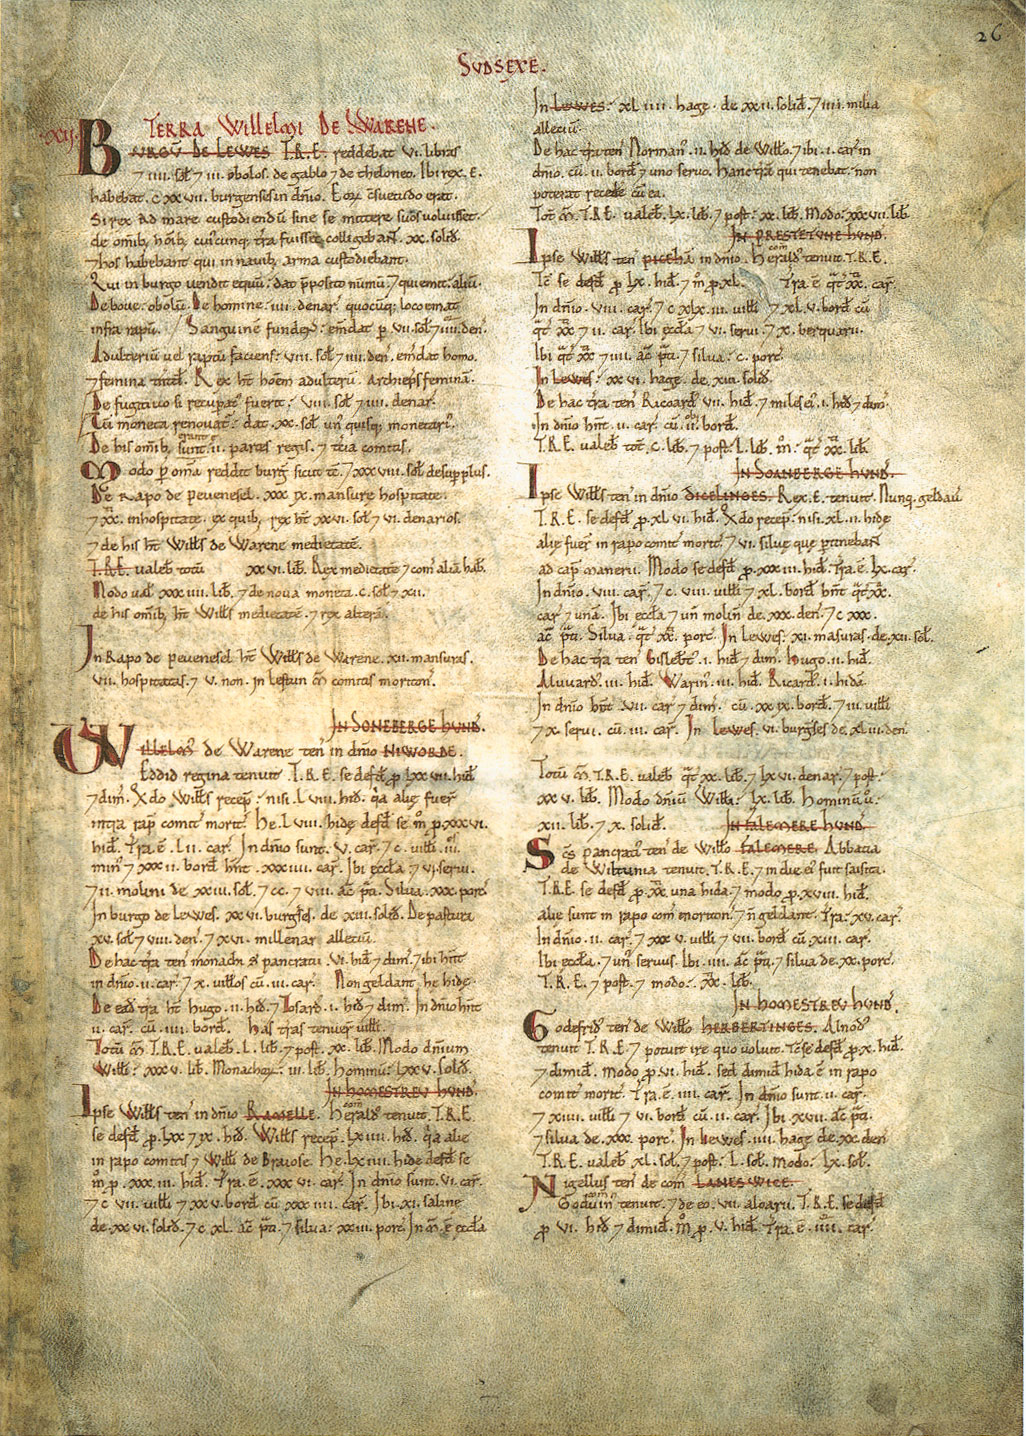
\includegraphics[width=0.75\linewidth]{images1/domesday} 

}

\caption{Domesday Book}\label{fig:unnamed-chunk-3}
\end{figure}

\hfill\break

1602

\hfill\break

O dramaturgo inglês William Shakespeare usou a palavra \textbf{statists} (estadistas e, portanto, num sentido não relacionado com números ou matemática) no diálogo da Cena II de Hamlet \href{http://shakespeare.mit.edu/hamlet/full.html}{(link)}.

\hfill\break

\begin{quote}
``Hamlet:
Cercado assim por tantas vilanias, mesmo antes de eu poder dizer o prólogo, representava o cérebro.
Sentei-me e escrevi com capricho nova carta. Já pensei, como os nossos estadistas, que é feio escrever bem, tendo insistido, até, em desaprendê-lo; mas, nessa hora muito bom me foi isso. Quererias saber
qual o conteúdo da mensagem?{[}\ldots{]}''
\end{quote}

\hfill\break

1603

\hfill\break

O negociante inglês John Graunt (1620-1674) substituiu a crença pela evidência em \emph{Natural and Political Observations Mentioned in a Following Index and Made upon the Bills of Mortality} (Observações naturais e políticas feitas sobre as notas de mortalidade).

Nesse trabalho, realizado com dados coletados das paróquias de Londres entre 1604 e 1660, Graunt tirou as seguintes conclusões: que havia maior nascimento de crianças do sexo masculino, mas havia distribuição aproximadamente igual de ambos os sexos na população geral; alta mortalidade nos primeiros anos de vida; maior mortalidade nas zonas urbanas em relação às zonas rurais.

\hfill\break

\begin{figure}

{\centering 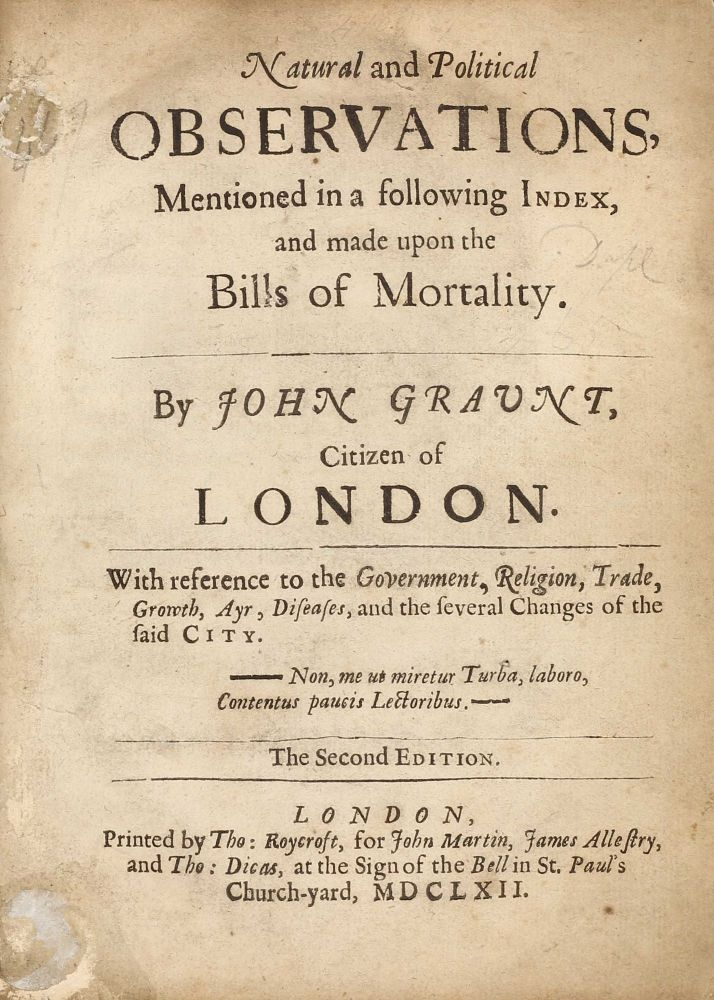
\includegraphics[width=0.75\linewidth]{images1/graunt} 

}

\caption{Natural and Political Observations Mentioned in a Following Index and Made upon the Bills of Mortality (ed. de 1662)}\label{fig:unnamed-chunk-4}
\end{figure}

\hfill\break

1660

\hfill\break

Herman Conring (1606-1681), professor de filosofia, medicina e política da Universidade de Helmstadt (atual Alemanha), criou um curso de Ciência política em 1660, que descrevia e examinava as questões fundamentais do Estado. Nele a \textbf{estatística} passou a ser considerada como uma disciplina autônoma que tinha por objetivo a descrição das coisas do Estado.

\hfill\break

1687

\hfill\break

Em 1687 o economista e filósofo inglês William Petty (1623-1687) publicou \emph{Five Essays on Political Arithmetic} (Cinco ensaios sobre aritmética política), sugerindo ao governo inglês a criação de um departamento para registro de \textbf{estatísticas} vitais.

\hfill\break

\begin{figure}

{\centering 
\includegraphics[width=0.75\linewidth]{images1/petty} 

}

\caption{Several Essays in Political Arithmetick (ed. de 1699)}\label{fig:unnamed-chunk-5}
\end{figure}

\hfill\break

O Capitão John Graunt e William Petty instituiram na Inglaterra um novo ramo de estudos denominado de \emph{Political arithmetic} (Aritmética política)

\hfill\break

1693

\hfill\break

O matemático e astrônomo inglês Edmond Halley (1656-1742) construiu em 1693, baseado em dados coletados na cidade (à época) alemã de Bresláu, uma \emph{Life Table} (Tábua de sobrevivência), um estudo que analisa as probabilidades de sobrevivência e morte em relação à idade.

\hfill\break

\begin{figure}

{\centering 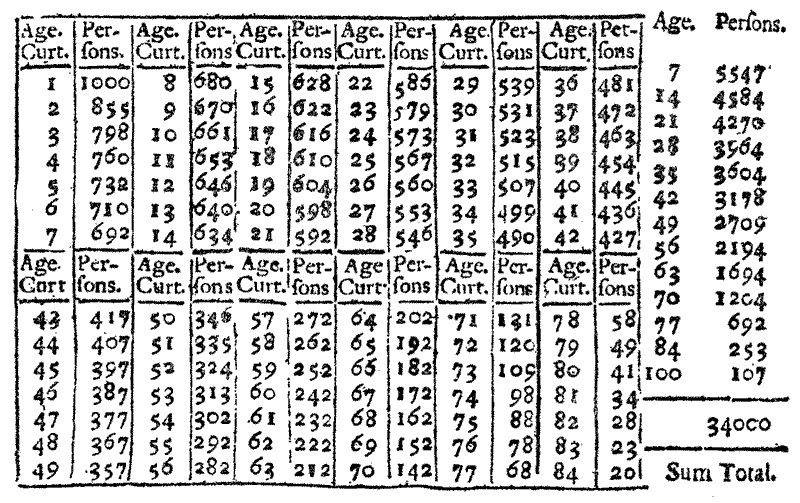
\includegraphics[width=0.75\linewidth]{images1/halley} 

}

\caption{Halley’s life table (1693)}\label{fig:unnamed-chunk-6}
\end{figure}

\hfill\break

1749

\hfill\break

Com um sentido não relacionado com números ou matemática, a palavra \textbf{estatística} parece ter sido proposta pela primeira vez no século XVII, pelo historiador e professor alemão (à época Transilvânia) Martin Schmeitzel (1679-1747) da Universidade de Jena e, posteriormente adotada por seu aluno, (igualmente) historiador e jurista Gottfried Achenwall (1719-1772) em 1749, em \emph{Abriß der neuen Staatswissenschaft der vornehmen Europäischen Reiche und Republiken} (Esboço da nova ciência política dos nobres impérios europeus e repúblicas).

\hfill\break

\begin{figure}

{\centering 
\includegraphics[width=0.75\linewidth]{images1/gottfried} 

}

\caption{Abriß der neuen Staatswissenschaft der vornehmen Europäischen Reiche und Republiken (1749)}\label{fig:unnamed-chunk-7}
\end{figure}

\hfill\break

1771

\hfill\break

William Hooper usou a palavra \textbf{estatística} em sua tradução de \emph{The Elements of Universal Erudition}(Elementos da Erudição Universal) escrita por Jacob Friedrich Freiherr von Bielfeld (1717-1770).

Nesse livro, a \textbf{estatística} foi definida como a ciência que nos ensina o arranjo político de todos os estados modernos do mundo conhecido (mais uma veznum sentido não associado a números ou matemática).

\hfill\break

\begin{figure}

{\centering 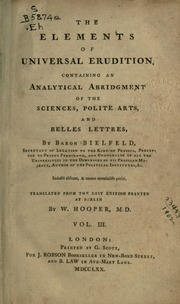
\includegraphics[width=0.75\linewidth]{images1/hooper} 

}

\caption{The Elements of Universal Erudition  (1771)}\label{fig:unnamed-chunk-8}
\end{figure}

\hfill\break

1790

\hfill\break

O jurista e político escocês John Sinclair propôs que se realizasse uma detalhada pesquisa em 938 paróquias para elucidar a história natural e política de seu país (\emph{Statistics Accounts}). Essa pesquisa fazia parte de um projeto muito mais ousado: \emph{The Pyramid of Statistical Enquiry} (A Pirâmide da Pesquisa Estatística).

\hfill\break

\begin{figure}

{\centering 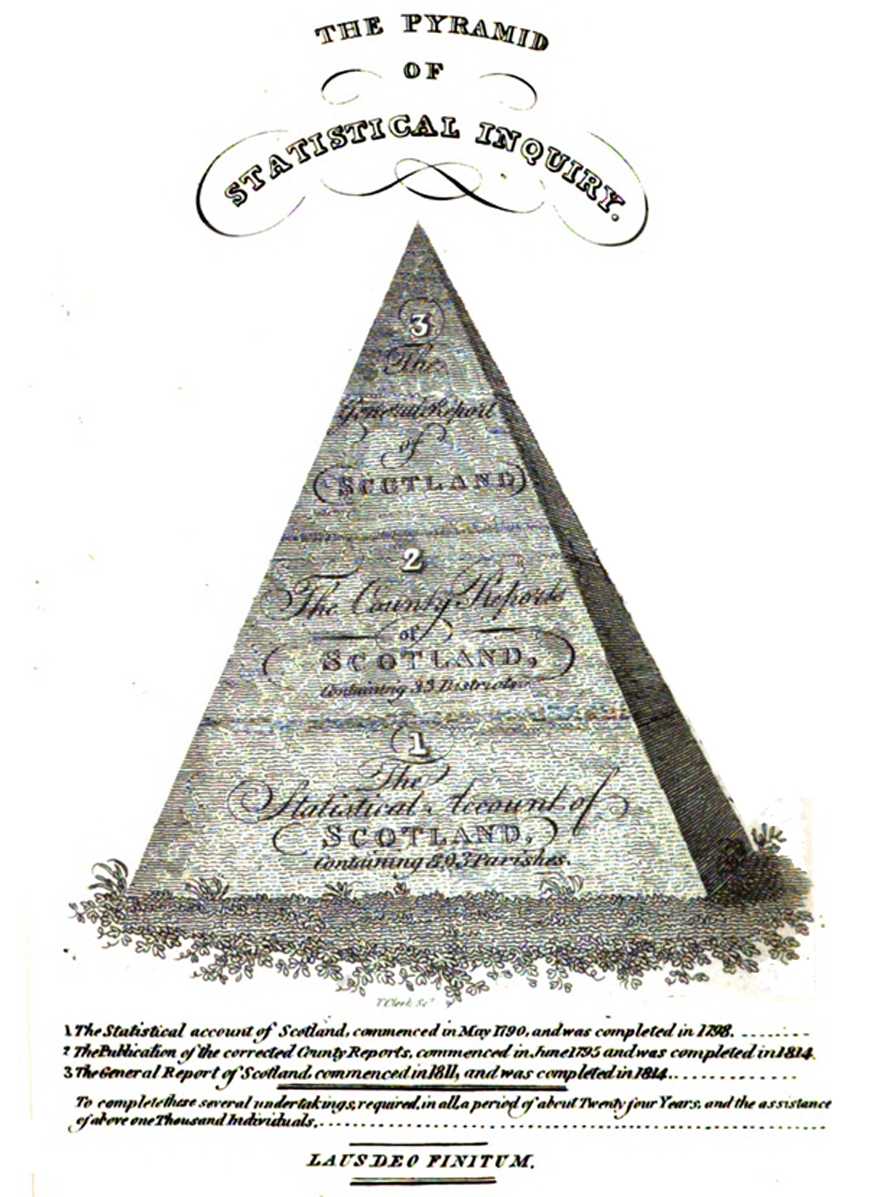
\includegraphics[width=0.75\linewidth]{images1/sinclair} 

}

\caption{The Pyramid of Statistical Enquiry  (1814)}\label{fig:unnamed-chunk-9}
\end{figure}

\hfill\break

1854

\hfill\break
O médico inglês (considerado por alguns como o ``pai'' da epidemiologia moderna) John Snow (1813-1858) estudou a dispersão espacial dos casos de cólera em Londres e concluiu que sua causa residia na contaminação da água consumida (poço localizado na \emph{Broad Street}, no distrito do \emph{Soho}): \emph{Report to the Cholera Outbreak in the Parish of St.~James, Westminster during the Autumn of 1854} (Relatório sobre o surto de cólera na paróquia de St.~James, Westminster durante o outono de 1854).

\hfill\break

\begin{figure}

{\centering 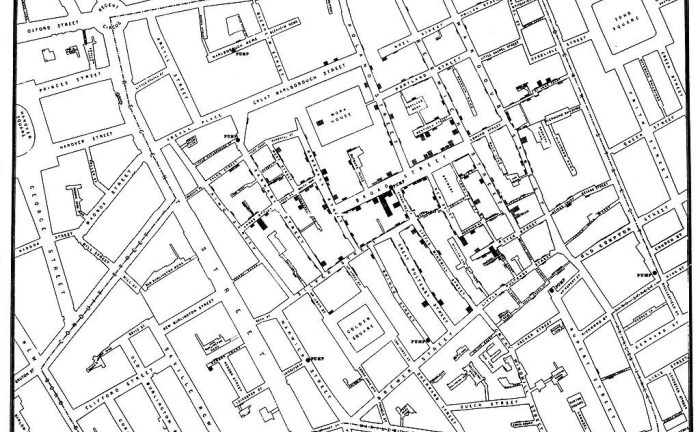
\includegraphics[width=0.75\linewidth]{images1/london-1854-snow} 

}

\caption{Mapa dos casos de cólera (1854)}\label{fig:unnamed-chunk-10}
\end{figure}

\hypertarget{visualizauxe7uxe3o-de-dados-estudos-e-primeiras-publicauxe7uxf5es}{%
\section{Visualização de dados \& Estudos e primeiras publicações}\label{visualizauxe7uxe3o-de-dados-estudos-e-primeiras-publicauxe7uxf5es}}

1765

\hfill\break

O teólogo e filósofo inglês Joseph Priestley (1733-1804) introduziu como inovação os primeiros gráficos com linha temporal, em que barras individuais eram usadas para visualizar o tempo de vida de uma pessoa e o todo pode ser usado para comparar a expectativa de vida de várias pessoas.

\hfill\break

\begin{figure}

{\centering 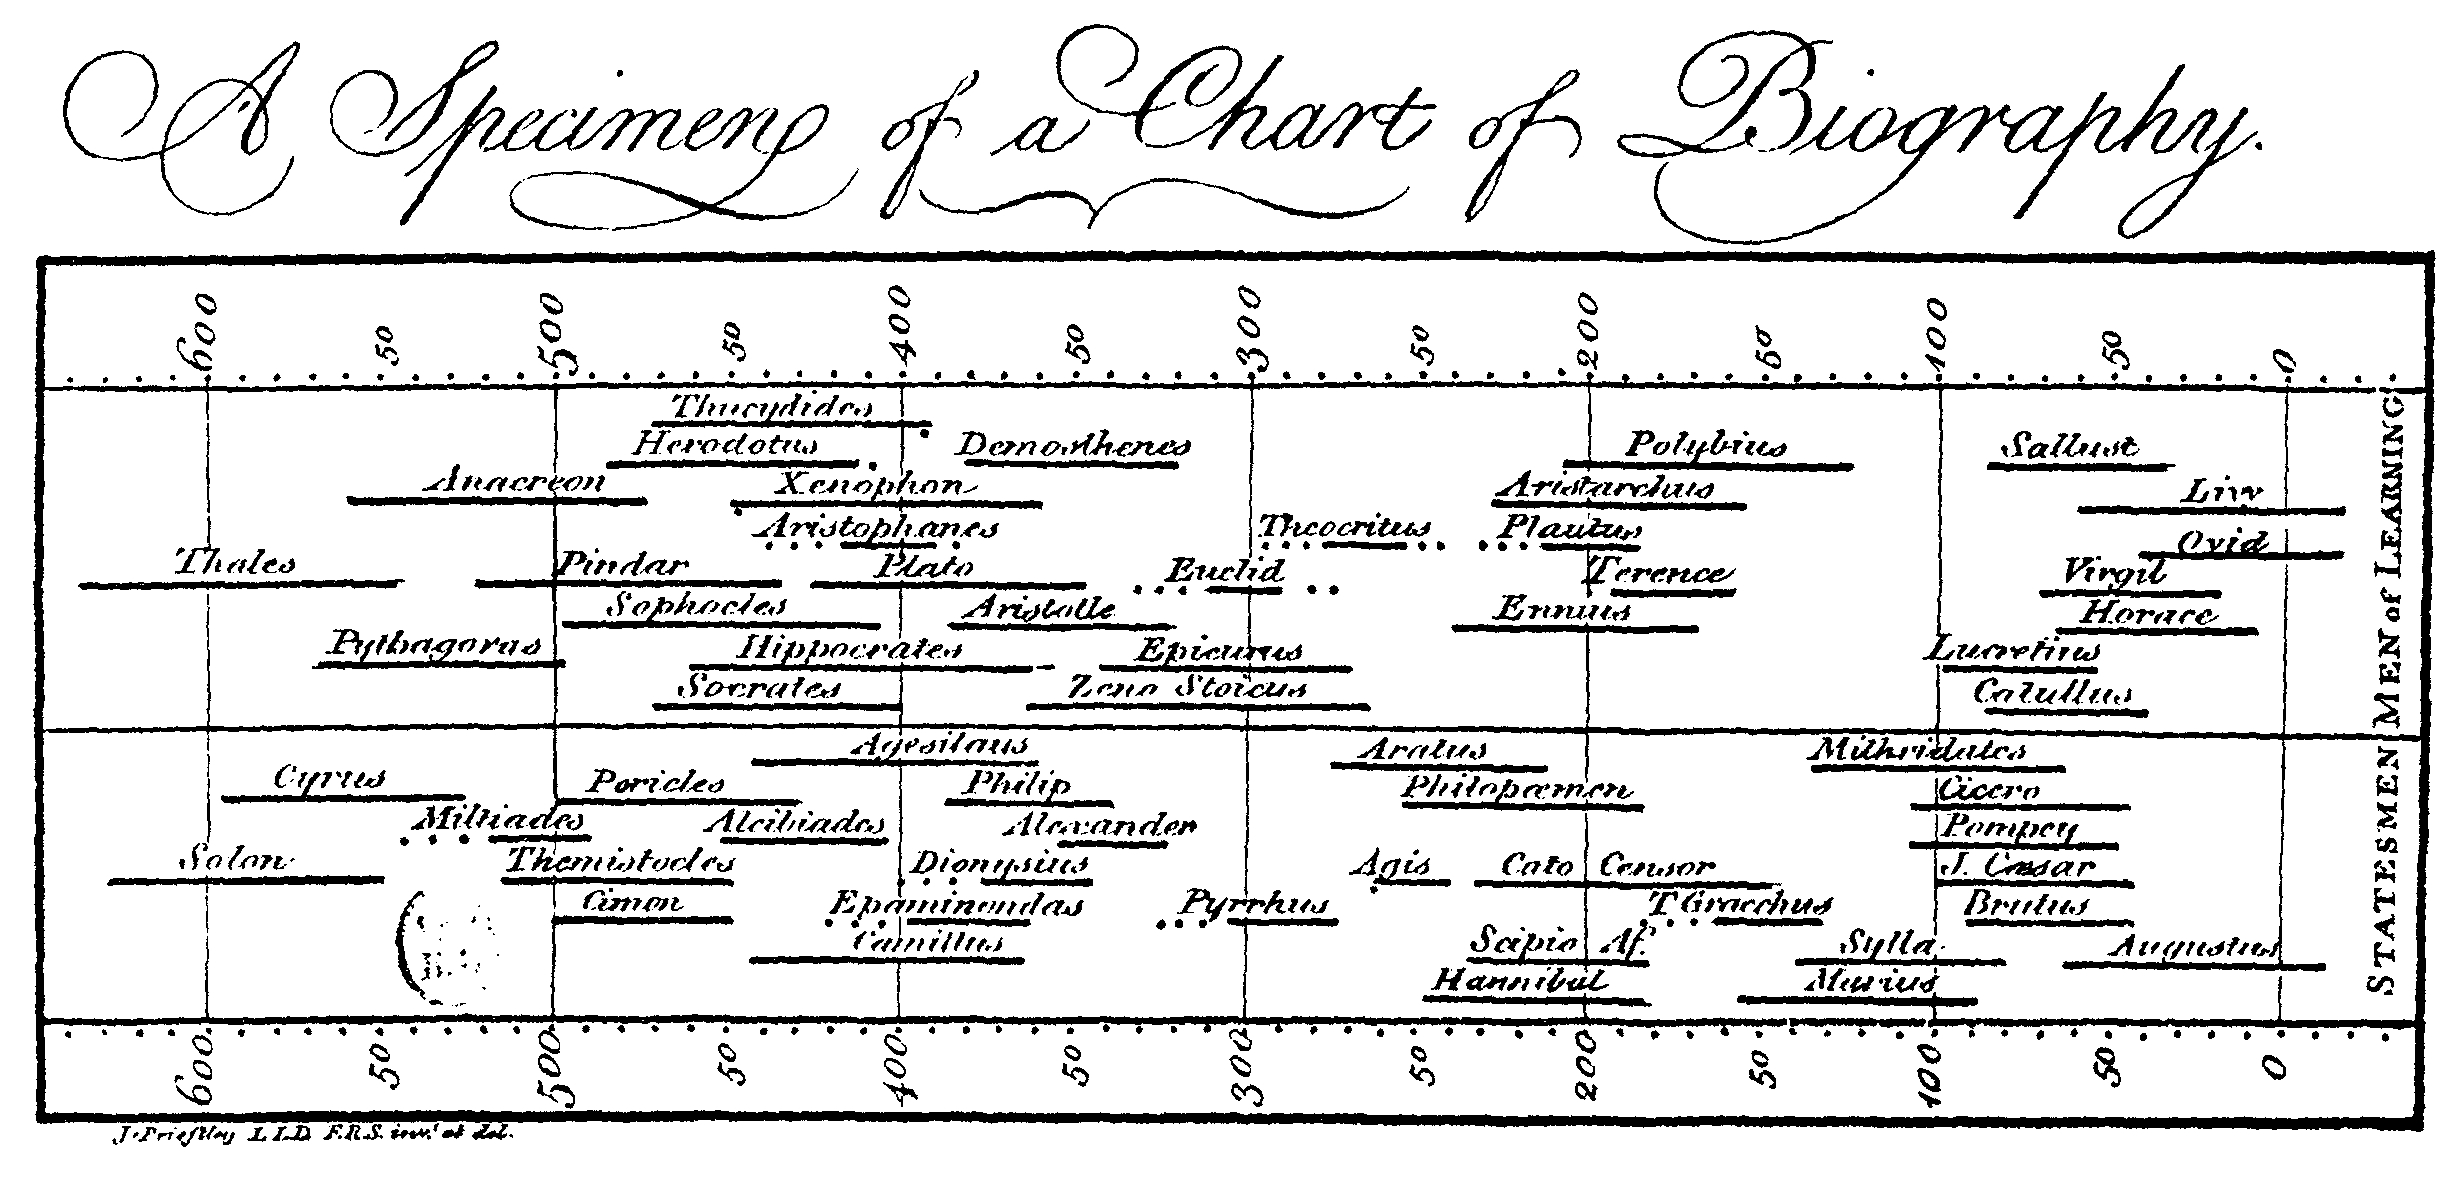
\includegraphics[width=0.75\linewidth]{images1/priestley-timechart-1765} 

}

\caption{Expectativa de vida de diversas pessoas (1765)}\label{fig:unnamed-chunk-11}
\end{figure}

\hfill\break

1786

\hfill\break

O engenheiro e economista escocês William Playfair (1759-1823) é considerado comumente como fundador dos métodos gráficos para apresentação de estatísticas. Playfair concebeu vários tipos de diagramas para visualização de dados:

\begin{itemize}
\tightlist
\item
  em 1786, o gráfico de barras; e,
\item
  em 1801, o gráfico de setores.
\end{itemize}

\hfill\break

\begin{figure}

{\centering 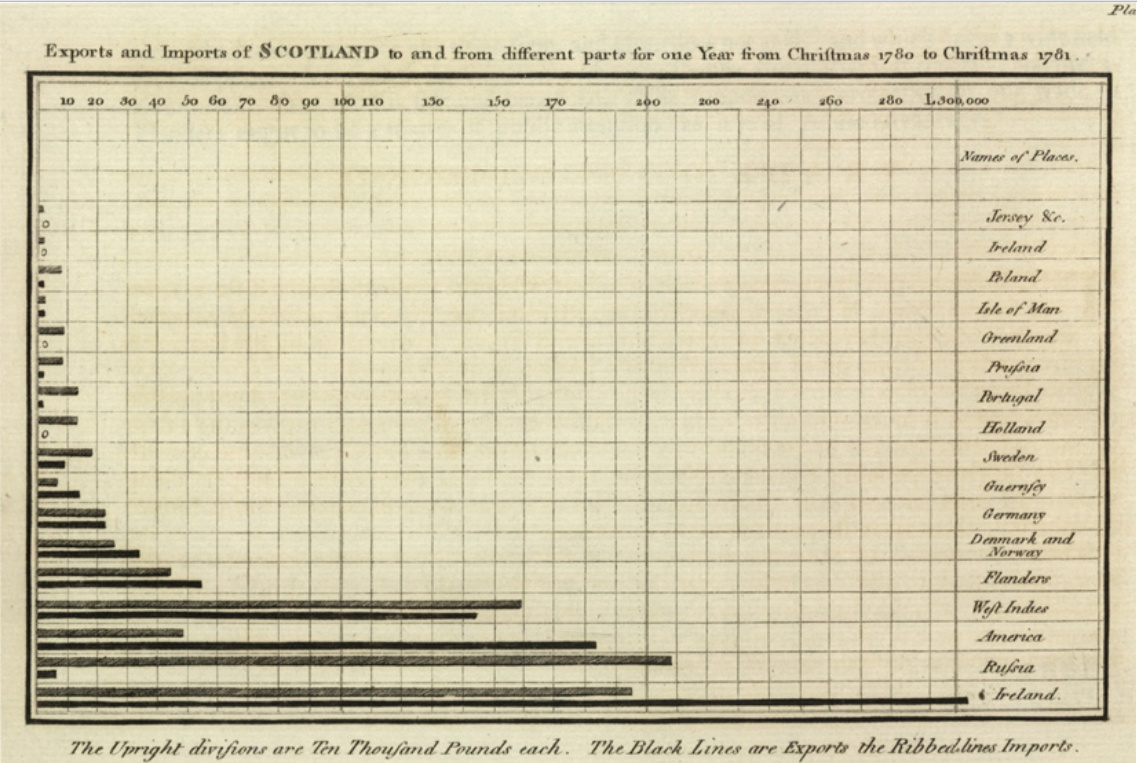
\includegraphics[width=0.75\linewidth]{images1/playfair-barchart-1786} 

}

\caption{Commercial and Political Atlas (Atlas Comercial e Político de 1786): cada barra representa as exportações e importações da Escócia para 17 países em 1781}\label{fig:unnamed-chunk-12}
\end{figure}

\hfill\break

\begin{figure}

{\centering 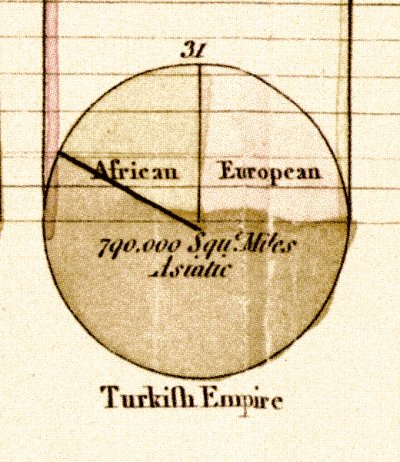
\includegraphics[width=0.75\linewidth]{images1/playfair-piechart-1801} 

}

\caption{Statistical Breviary (Breviário Estatístico de 1801): proporção da extensão do Império Turco em diferentes regiões do mundo: Asia, Europa e África, antes de 1789}\label{fig:unnamed-chunk-13}
\end{figure}

\hfill\break

1856

\hfill\break

A enfermeira inglesa Florence Nightingale (1820-1910) conduziu um trabalho pioneiro ao chegar no hospital militar britânico na Turquia em 1856, estabelecendo uma ordem e um método muito necessários aos registros médicos estatísticos e que indicaram serem as precárias práticas sanitárias o culpado da alta mortalidade \href{https://www.york.ac.uk/depts/maths/histstat/small.htm}{(link)}.

\hfill\break

\begin{figure}

{\centering 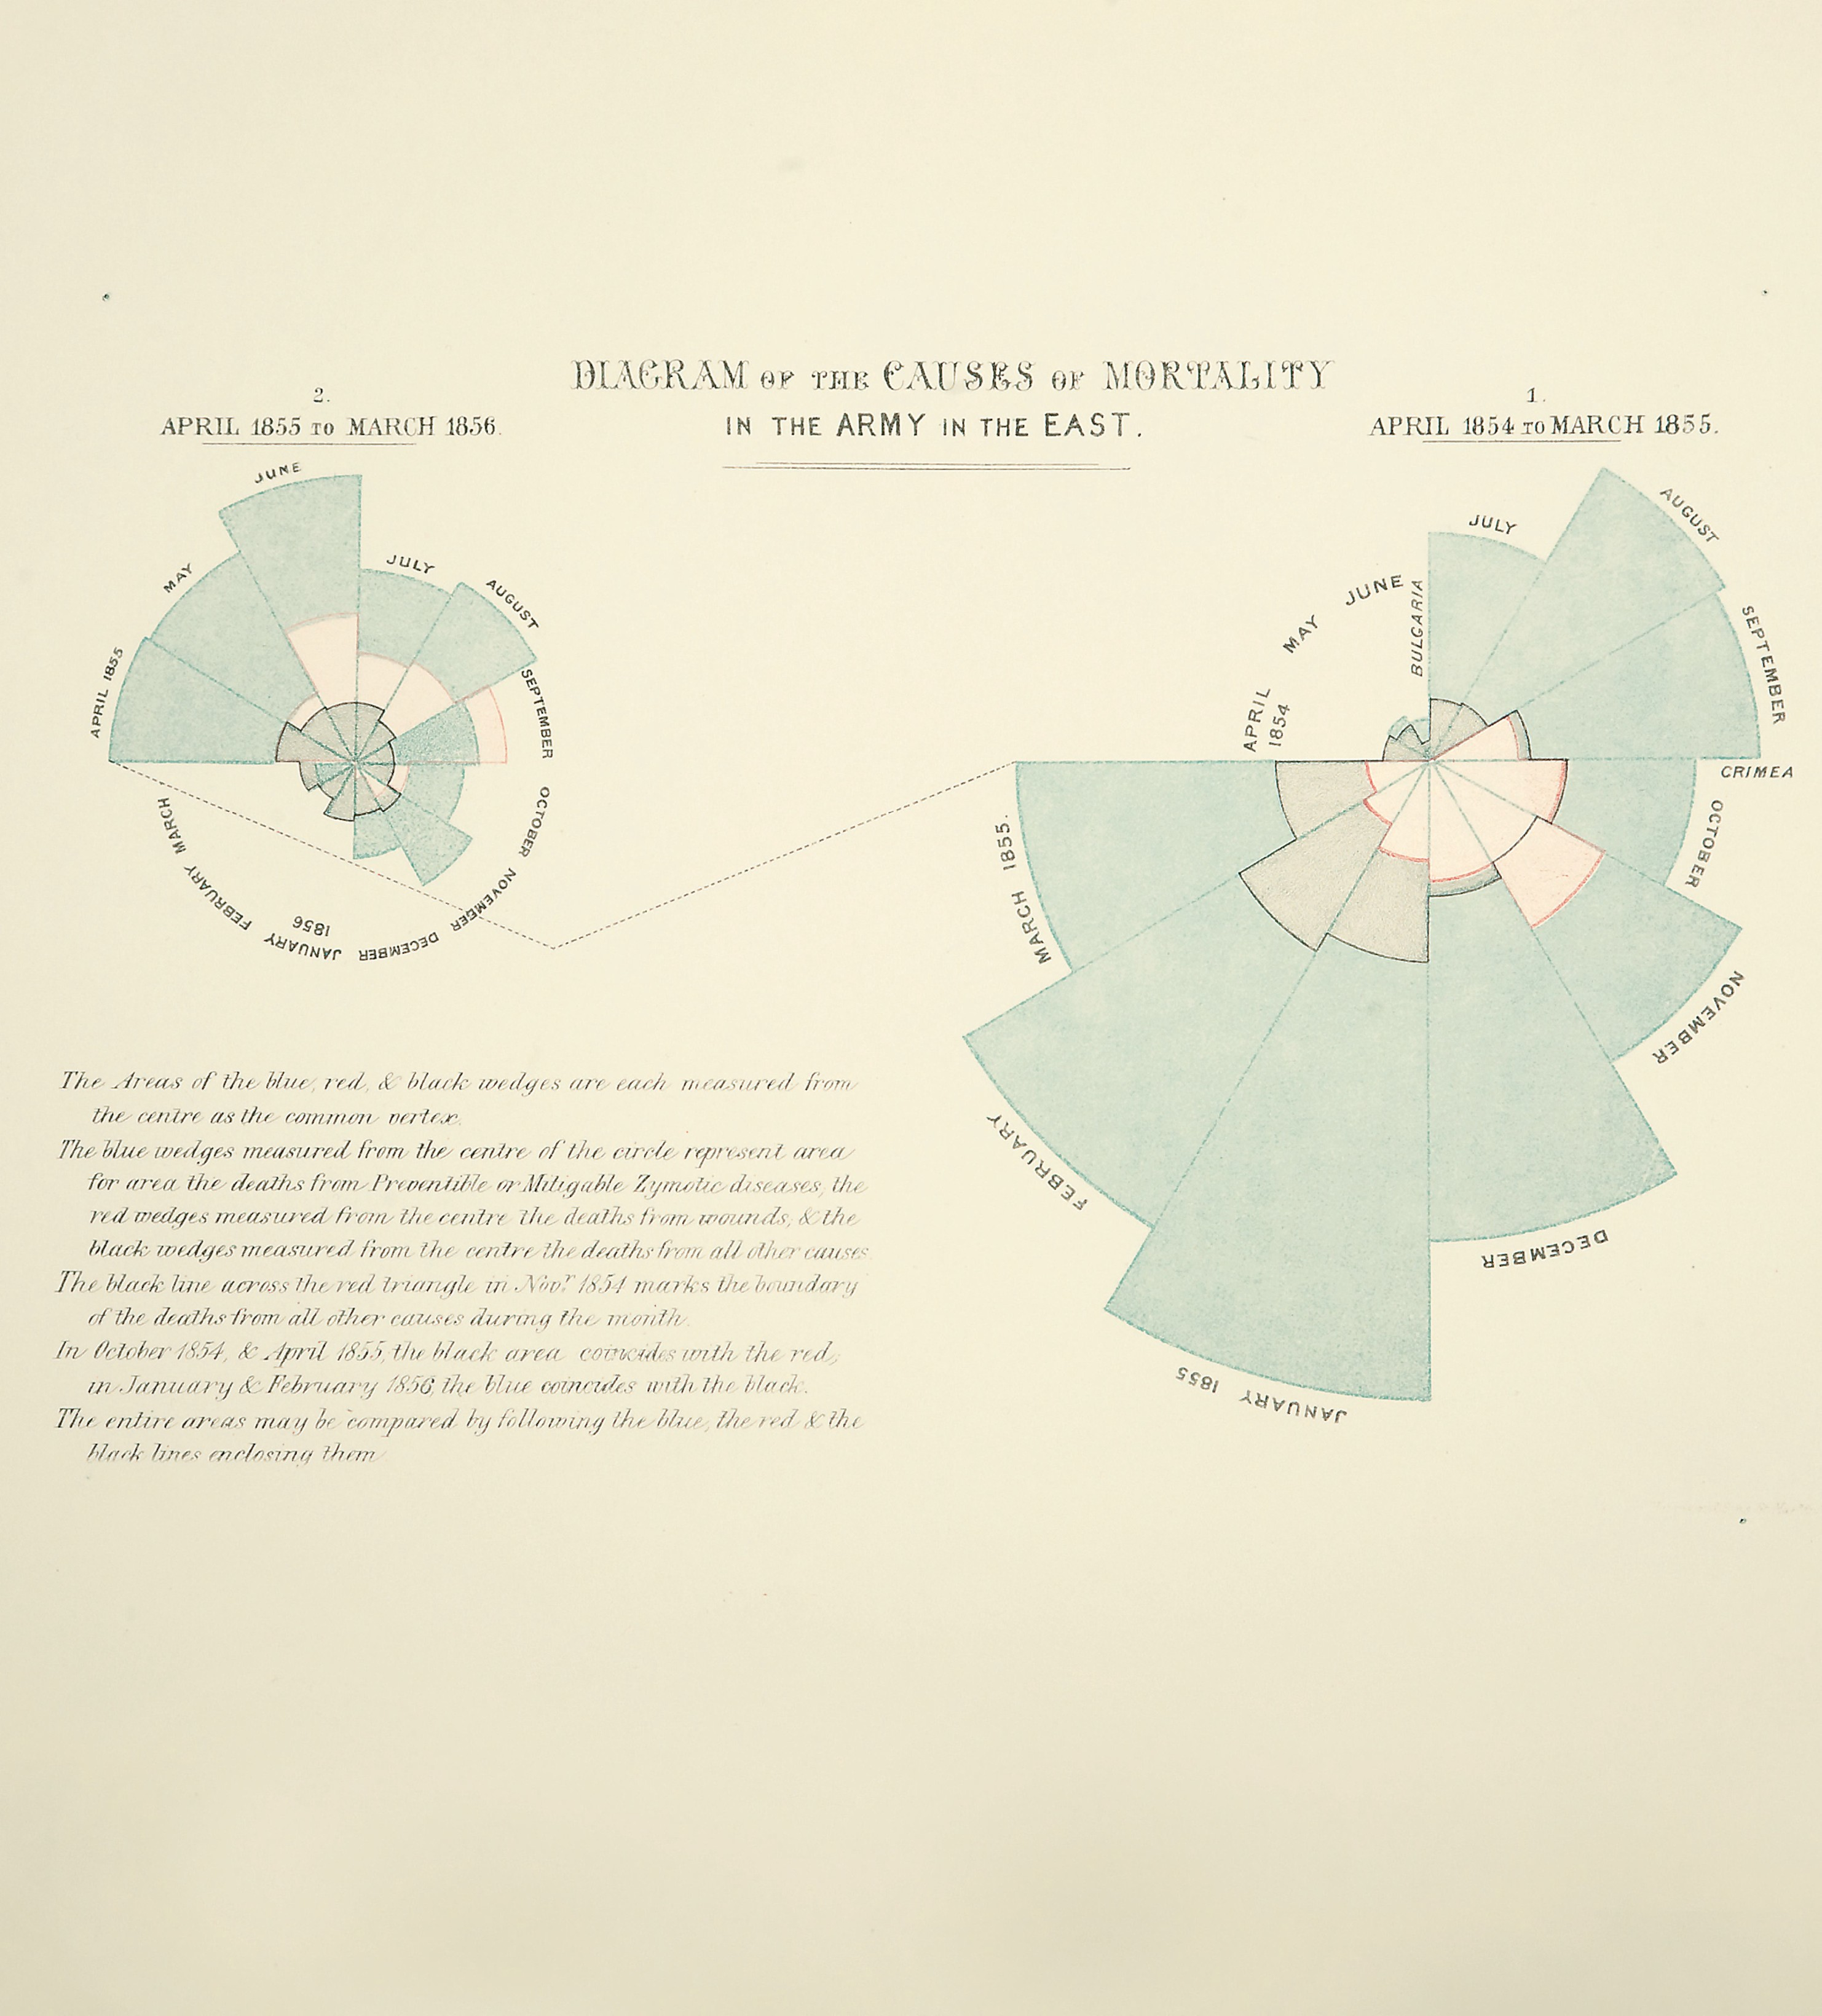
\includegraphics[width=0.75\linewidth]{images1/florence-rose-diagram} 

}

\caption{Esse diagrama (coxcomb) feito durante a Guerra da Crimeia foi dividido igualmente em 12 setores, representando os meses do ano, com a área sombreada do setor  de cada mês proporcional à taxa de mortalidade naquele mês. Seu sombreamento com código de cores indicava a causa da morte em cada área do diagrama}\label{fig:unnamed-chunk-14}
\end{figure}

\hfill\break

\begin{figure}

{\centering 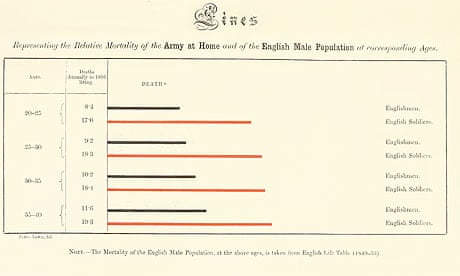
\includegraphics[width=0.75\linewidth]{images1/florence-barr} 

}

\caption{Gráfico de barras de Florence Nightingale mostrando as diferenças de mortalidade entre soldados britânicos e a população masculina inglesa geral (civis)}\label{fig:unnamed-chunk-15}
\end{figure}

\hfill\break

\hypertarget{nomes-notuxe1veis}{%
\section{Nomes notáveis}\label{nomes-notuxe1veis}}

Karl Pearson (1857-1936) é amplamente considerado o fundador da disciplina moderna de \textbf{estatística}, e também é famoso como um filósofo da ciência, como escritor sobre o darwinismo social e como um dos principais impulsionadores para instalar a eugenia como a ciência social chave. Uma breve biografia de cada um dos pesquisadores a seguir relacionados pode ser obtida em: \href{http://www-history.mcs.st-andrews.ac.uk/BiogIndex.html}{(link)}.

\begin{itemize}
\tightlist
\item
  Niccolò Fontana Tartaglia (Veneza à época, hoje Itália: 1499-1557)
\item
  Girolamo Cardano (Pávia à época, hoje Itália: 1501-1576)
\item
  Galileu Galilei (Florença à época, hoje Itália: 1564-1642)
\item
  Pierre de Fermat (França: 1607-1665)
\item
  Blaise Pascal (França: 1623-1662)
\item
  Jakob Bernoulli (Suíça: 1655-1705)
\item
  Abrahan de Moivre (França: 1667-1754)
\item
  Thomas Bayes (Inglaterra: 1702-1761)
\item
  Pierre-Simon Laplace (França: 1749-1827)
\item
  Johann Carl Friedrich Gauss (Alemanha: 1777-1856)
\item
  Lambert Adolphe Jacques Quételet (França à época, hoje Bélgica: 1796-1874)
\item
  Pafnuti Lvovitch Chebyshev (Rússia: 1821-1894)
\item
  Francis Galton (Inglaterra: 1822-1911)
\item
  Wilhelm Lexis (Alemanha: 1837-1914)
\item
  Thorvald Nicolai Thiele (Dinamarca: 1838-1910)
\item
  Friedrich Robert Helmert (Saxônia: 1843-1917)
\item
  Francis Ysidro Edgeworth (Inglaterra: 1845-1926)
\item
  James Douglas Hamilton Dickson (Escócia: 1849-1931)
\item
  Andrei Andreyevich Markov (Rússia: 1856-1922)
\item
  Aleksandr Mikhailovich Lyapunov (Rússia: 1857-1918)
\item
  Walter Frank Raphael Weldon (Inglaterra: 1860-1906)
\item
  Karl Pearson (Inglaterra: 1857-1936)
\item
  William Seally Gosset (Inglaterra: 1876-1937)
\item
  Ronald Aylmer Fisher (Inglaterra: 1890-1962)
\item
  Andrei Nikolaevich Kolmogorov (Rússia: 1903-1987)
\end{itemize}

\hypertarget{revista-biometrika}{%
\section{Revista Biometrika}\label{revista-biometrika}}

\hfill\break

\begin{quote}
``Pretende-se que a \emph{Biometrika} sirva como um meio não apenas de coletar ou publicar, sob um título, dados biológicos de um tipo não coletados sistematicamente ou publicados em outro lugar em qualquer outro periódico, mas também de disseminar um conhecimento de tal teoria estatística para o seu tratamento científico{[}\ldots{]}''
\end{quote}

\hfill\break

Em outubro de 1901 foi fundada a \emph{Biometrika, the Journal for the Statistical Study of Biological Problems} (Biometrika, o Jornal para o Estudo Estatístico de Problemas Biológicos) com o propósito de promover a análise estatística de fenômenos biológicos, isto é, a matematização da biologia.

Os fundadores da \emph{Biometrika} foram \emph{Sir} Francis Galton (primo de Charles Darwin), Walter Frank Raphael Weldon e Karl Pearson. A maior parte do trabalho foi feita por Pearson e Weldon, este último focando na edição do conteúdo (ou seja, o aspecto biológico) e o primeiro nos detalhes, incluindo correções de prova. Galton e o eugenista americano Charles Davenport atuaram, respectivamente, como consultor e editor.

Alguns dos tópicos abordados na revista incluem criminologia, botânica, zoologia, epidemiologia e outros aspectos da saúde humana. Na década de 1930, o caráter da \emph{Biometrika} mudou, e ``representou a vanguarda internacional da pesquisa em métodos estatísticos e sua aplicação na ciência e tecnologia'\,', ao invés de focar a hereditariedade.

\emph{Sir} Francis Galton, que serviu como editor da primeira edição (1901), escreveu a Introdução, que incluiu uma declaração de propósito para a revista\\
\href{https://academic.oup.com/biomet/article-abstract/1/1/1/192192?redirectedFrom=fulltext}{(link)}.

\hypertarget{eugenia}{%
\section{Eugenia}\label{eugenia}}

Em 16 de maio de 1883 \emph{Sir} Francis Galton cunhou o termo ``eugenia'', posteriormente descrevendo-o como ``o estudo das agências sob controle social que podem melhorar ou reparar as qualidades raciais das gerações futuras, seja fisicamente ou mentalmente''.

Galton detalha o conceito em seu livro \emph{Inquiries into Human Faculty and its Development}, e recomenda que indivíduos de famílias altamente classificadas em seu sistema de mérito sejam encorajados a se casar cedo e receber incentivos para ter filhos. Ele também condenou os casamentos tardios dentro desse mesmo grupo como ``disgênicos'' ou desvantajosos para a espécie humana.

A palavra ``eugenia'' foi extraída da palavra grega \emph{eu}, que significa bem, e \emph{genos}, que significa prole. Juntos, significa bem-nascido.

Este livro caiu em domínio público e pode ser lido na íntegra online. A caracterização original de eugenia de Galton pode ser encontrada na página 17 desta edição de domínio público (Parte 1 do pdf):

\hfill\break

\begin{quote}
``uma breve palavra para expressar a ciência de melhorar o rebanho, que não está de modo algum confinado a questões de acasalamento criterioso, mas que, especialmente no caso do homem, toma conhecimento de todas as influências que tendem, mesmo que em grau remoto, a dar ao raças ou linhagens de sangue mais adequadas uma melhor chance de prevalecer rapidamente sobre os menos adequados do que teriam de outra forma {[}\ldots{]}''(Galton, 1883, p.17)
\end{quote}

\hfill\break

Há poucos anos alguns grupos sociais viram no trabalho e opiniões de Fisher endossos ao colonialismo, à supremacia branca e à eugenia.

Outros grupos, todavia, afirmam que Fisher não era racista e eugenista, embora ele achasse que havia diferenças comportamentais e de inteligência entre os grupos humanos.

\hfill\break

\begin{figure}

{\centering 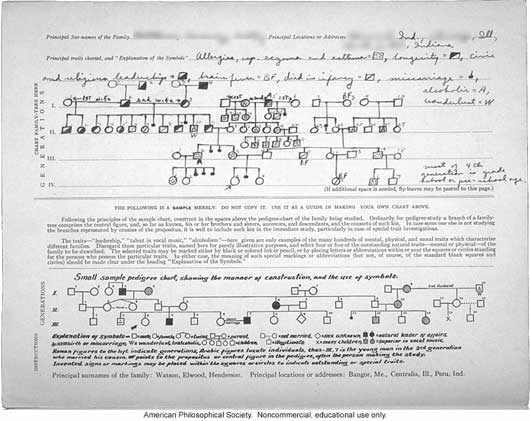
\includegraphics[width=0.75\linewidth]{images1/chart_pedigree_allergy2} 

}

\caption{Gráfico de linhagens para alergias}\label{fig:unnamed-chunk-16}
\end{figure}

\hfill\break

\begin{figure}

{\centering 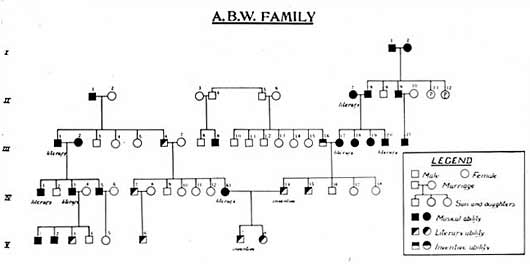
\includegraphics[width=0.75\linewidth]{images1/chart_pedigree_music2 (1)} 

}

\caption{Gráfico de linhagens para aptidão musical}\label{fig:unnamed-chunk-17}
\end{figure}

\hfill\break

\begin{figure}

{\centering 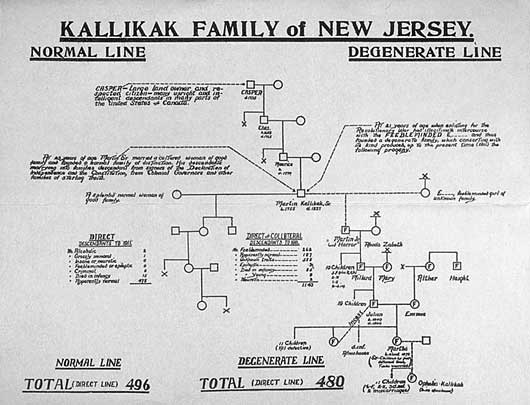
\includegraphics[width=0.75\linewidth]{images1/chart_Kallikak_pedigree2} 

}

\caption{Linhas "normais" e "degeneradas" da família Kallikak (New Jersey)}\label{fig:unnamed-chunk-18}
\end{figure}

\hfill\break

\begin{figure}

{\centering 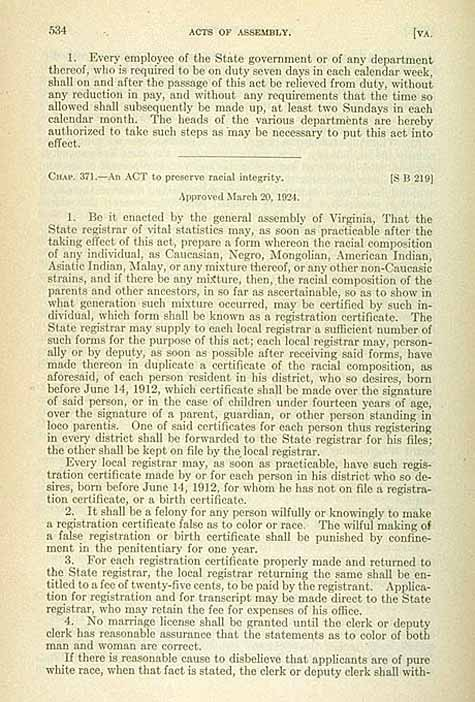
\includegraphics[width=0.75\linewidth]{images1/VA_racial_integrity_act2} 

}

\caption{Lei da Inegridade Racia (Virginia, EUA, 1924)}\label{fig:unnamed-chunk-19}
\end{figure}

\hfill\break

\begin{figure}

{\centering 
\includegraphics[width=0.75\linewidth]{images1/choosing_love_over_eugenics} 

}

\caption{Licença para casamento}\label{fig:unnamed-chunk-20}
\end{figure}

\hypertarget{conceitos_gerais}{%
\chapter{- Introdução conceitual essencial}\label{conceitos_gerais}}

\begin{quote}
``Estatística é um conjunto de métodos que se destina a possibilitar a tomada de decisões, face às incertezas{[}\ldots{]}'\,'
\end{quote}

De modo geral, a estatística pode ser dividida em três grandes áreas:

\begin{itemize}
\tightlist
\item
  descritiva;
\item
  probabilidade; e,
\item
  inferencial.
\end{itemize}

\hypertarget{estatuxedstica-descritiva}{%
\section{Estatística descritiva}\label{estatuxedstica-descritiva}}

Nos primeiros trabalhos estatísticos, os dados coletados eram inicialmente apresentados na forma de tabelas e gráficos.

A \textbf{estatística descritiva} se ocupa de tudo o que seja relacionado a dados: coleta, processamento, descrição (seja na forma tabular ou gráfica) e sínteses numéricas (de locação, de dispersão, de repartição) sem inferir coisa alguma além da informação trazida pelos dados. Vem experimentando crescente uso em todas as áreas científicas e desenvolvimento:

\begin{itemize}
\tightlist
\item
  crescente uso de uma abordagem quantitativa em todas as ciências;
\item
  disponibilidade de recursos computacionais;
\item
  quantidade de dados coletados.
\end{itemize}

A palavra \textbf{estatística} pode assumir diferentes significados:

\begin{itemize}
\tightlist
\item
  no singular: \textbf{estatística} \vspace{0.5cm}

  \begin{itemize}
  \tightlist
  \item
    refere-se à ciência que compreende métodos que são usados na coleta, análise, interpretação e apresentação de dados quantitativos ou qualitativos (numéricos ou não); e,
  \item
    denota uma medida ou fórmula específica (tais como uma média, um intervalo de valores, uma taxa de crescimento, um índice).
  \end{itemize}
\item
  no plural: \textbf{estatísticas}

  \begin{itemize}
  \tightlist
  \item
    refere-se a dados coletados de maneira sistemática com um propósito específico definido em qualquer campo de estudo (nesse sentido, as \emph{estatísticas} também podem ser consideradas como agregados de fatos expressos em forma numérica).
  \end{itemize}
\end{itemize}

\hypertarget{estatuxedstica-inferencial}{%
\section{Estatística inferencial}\label{estatuxedstica-inferencial}}

A \textbf{estatística inferencial} tem o objetivo de estabelecer níveis de confiança da tomada de decisão de associar uma estimativa amostral a um parâmetro populacional. Divide-se em estimação e testes de significância.

\begin{quote}
``Dedução e indução são procedimentos racionais que nos levam do já conhecido ao ainda não conhecido; isto é, permitem que adquiramos conhecimentos novos graças a conhecimentos já adquiridos.{[}\ldots{]}''
\end{quote}

Dedução.

Na dedução parte-se de uma verdade já conhecida para demonstrar que ela se aplica a todos os casos particulares iguais. Vai do geral ao particular.

Indução.

Na indução parte-se de alguns casos particulares iguais ou semelhantes para se estipular uma \textbf{lei geral}. Vai do particular ao geral.

Na dedução, dado \textbf{X}, infiro (concluo) \textbf{a}, \textbf{b}, \textbf{c}, \textbf{d}.

Na indução, dados \textbf{a}, \textbf{b}, \textbf{c}, \textbf{d}, infiro (concluo) \textbf{X}.

\begin{quote}
Exemplo: testes de aceleração (0-60 mph) feitos com 6 carros importados em 1999 resultaram nas seguintes medidas: 12,9 s; 16,50 s; 11,30 s; 15,20 s; 18,20 s e 17,70 s. Um estudo descritivo poderia afirmar que:
\end{quote}

\begin{itemize}
\tightlist
\item
  metade dos dados coletados acelera de 0-60 mph em menos de 16,00 s; e
\item
  a aceleração média de 0-60 mph é de 15,30 s.
\end{itemize}

\begin{quote}
Mas, a partir dessa amostra concluir que a aceleração média de \textbf{todos} os carros importados em 1999 seja de 15,30 s; ou, que \textbf{metade} dos carros importados em 1999 acelerem de 0-60 mph em menos de 16,00 s são afirmações que pertencem à \textbf{inferência estatística}.
\end{quote}

\hypertarget{produuxe7uxe3o-de-conhecimento}{%
\section{Produção de conhecimento}\label{produuxe7uxe3o-de-conhecimento}}

\begin{figure}

{\centering \includegraphics[width=1\linewidth]{images2/flux-george} 

}

\caption{Fluxograma elementar de um processo de aprendizagem}\label{fig:unnamed-chunk-22}
\end{figure}

Na expansão de qualquer área do conhecimento propomos hipóteses que serão avaliadas mediante a coleta de dados que, depois de analisados, revelarão informações que, eventualmente, nos conduzirão ao afastamento da hipótese original e à proposição de outras, num processo contínuo como, por exemplo:

\begin{enumerate}
\def\labelenumi{(\Alph{enumi})}
\tightlist
\item
\end{enumerate}

\begin{itemize}
\tightlist
\item
  Hipótese (ideia, teoria, conjectura): ``Hoje será um dia como outro qualquer.''
\item
  Dedução: ``Meu carro estará estacionado na garagem, no local de costume.''
\item
  Dados (informação, fatos): ``Meu carro não está lá!''
\item
  Inferência: ``Alguém deve tê-lo levado.''
\end{itemize}

\begin{enumerate}
\def\labelenumi{(\Alph{enumi})}
\setcounter{enumi}{1}
\tightlist
\item
\end{enumerate}

\begin{itemize}
\tightlist
\item
  Hipótese (ideia, teoria, conjectura): ``Meu carro foi roubado!''
\item
  Dedução: ``Meu carro não estará no local de costume.''
\item
  Dados (informação, fatos): ``Meu carro está lá!''
\item
  Inferência: ``Alguém deve tê-lo levado e devolvido.''
\end{itemize}

\begin{enumerate}
\def\labelenumi{(\Alph{enumi})}
\setcounter{enumi}{2}
\tightlist
\item
\end{enumerate}

\begin{itemize}
\tightlist
\item
  Hipótese (ideia, teoria, conjectura): ``Um ladrão pegou e trouxe de volta.''
\item
  Dedução: ``Meu carro foi arrombado.''
\item
  Dados (informação, fatos): ``Meu carro está intacto e o alarme está desligado.''
\item
  Inferência: ``Alguém que tenha as chaves deve tê-lo levado.''
\end{itemize}

\begin{enumerate}
\def\labelenumi{(\Alph{enumi})}
\setcounter{enumi}{3}
\tightlist
\item
\end{enumerate}

\begin{itemize}
\tightlist
\item
  Hipótese (ideia, teoria, conjectura): ``Minha esposa usou meu carro.''
\item
  Dedução: ``Ela provavelmente deixou um bilhete.''
\item
  Dados (informação, fatos): ``Sim, aqui está o bilhete.''
\item
  Inferência: ``Minha hipótese estava correta.''
\end{itemize}

Uma investigação científica deve envolver, em linhas gerais:

\begin{itemize}
\tightlist
\item
  observação dos fatos;
\item
  descrição das características essenciais, segundo o que se obteve através da observação;
\item
  explicação dessas características descritivas;
\item
  previsão; e,
\item
  decisão pertinente à investigação.
\end{itemize}

O planejamento de uma pesquisa deve envolver, em linhas gerais:

\begin{itemize}
\tightlist
\item
  definição do \emph{universo}\}: é necessário delimitar claramente, no tempo e espaço, o âmbito do inquérito, definindo, em termos precisos, o \emph{universo} a ser trabalhado;
\item
  exame das informações disponíveis: deve-se reunir todo o material existente: mapas, artigos, livros, relatórios relativos a levantamentos semelhantes;
\item
  tipos de levantamentos: completo ou amostral;
\item
  prazo;
\item
  custo;
\item
  precisão.
\end{itemize}

\hypertarget{populauxe7uxe3o-universo-amostra}{%
\section{População (universo) \& amostra}\label{populauxe7uxe3o-universo-amostra}}

\begin{figure}

{\centering 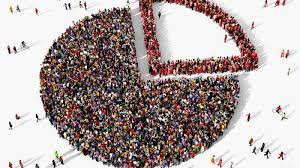
\includegraphics[width=1\linewidth]{images2/amostragem} 

}

\caption{Universo e amostra}\label{fig:unnamed-chunk-23}
\end{figure}

Quase que, invariavelmente, em todo ramo de conhecimento, o pesquisador esbarra em uma séria de limitações das mais variadas ordens (econômica, técnica, ética, geográfica, temporal,\ldots) que impossibilitam o estudo dos dados e informações associados a todos os casos existentes (\textbf{população ou universo}).

Por essa razão, através de um procedimento estatístico denominado de amostragem, estuda-se uma população (universo) a partir de uma amostra. Amostra é, portanto, um subconjunto finito e representativo da população (universo), extraído de modo sistemático (planejado).

\hypertarget{paruxe2metros-e-estatuxedsticas}{%
\section{Parâmetros e estatísticas}\label{paruxe2metros-e-estatuxedsticas}}

É comum a adoção de letras gregas para as características descritivas que se referirem à poúlação (universo) e letras do alfabeto latino para aquelas relativas à amostra extraída:

\begin{longtable}[]{@{}lll@{}}
\toprule()
Característica estudada & Notação populacional & Notação amostral \\
\midrule()
\endhead
Número de elementos & N & n \\
Média & \(\mu\) & \(\stackrel{-}{x}\) \\
Variância & \(\sigma^{2}\) & \({s}^{2}\) \\
Desvio padrão & \(\sigma\) & s \\
Proporção & \(\Pi\) & p \\
\bottomrule()
\end{longtable}

\begin{figure}

{\centering 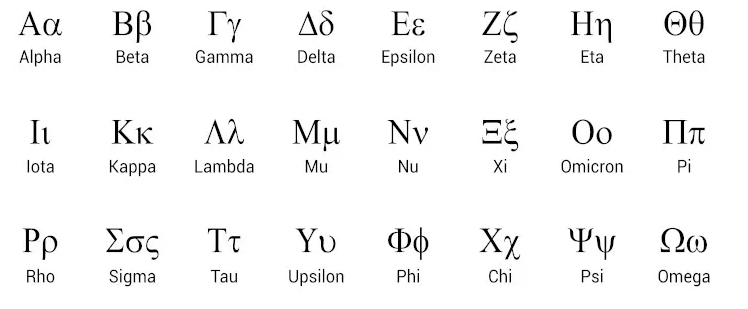
\includegraphics[width=1\linewidth]{images2/alf_grego} 

}

\caption{Alfabeto grego}\label{fig:unnamed-chunk-24}
\end{figure}

\hypertarget{tipos-de-variuxe1veis}{%
\section{Tipos de variáveis}\label{tipos-de-variuxe1veis}}

Variáveis quantitativas

\begin{itemize}
\tightlist
\item
  contínuas: são os dados com maior potencial de produzir informação significativa dentre todos: comprimentos, áreas, pesos, densidades; e,
\item
  discretas: são dados com um pouco menos de informação que os de natureza contínua mas possuem mais informação que dados qualitativos: número de andares de um prédio, de degraus de uma escada, número de filhos de um casal.
\end{itemize}

Variáveis qualitativas

\begin{itemize}
\tightlist
\item
  ordinais: apresentam um pouco mais de informação que os dados qualitativos puramente nominais na medida que suas classes podem ser interpretadas como possuindo um ordenamento inerente: padrão construtivo (baixo, médio, alto), classe econômica de rendimento (baixa, média, alta), nível de escolaridade (fundamental, médio e superior); e,
\item
  nominais: são dados a menor quantidade de informação: sexo, cor, códigos postais de cidades;
\end{itemize}

Codificação de variáveis qualitativas

\begin{itemize}
\tightlist
\item
  binárias: pela associação de valores numéricos: 0 ou 1 a uma variável qualitativa nominal que se apresente com apenas dois aspectos: sim ou não, ausência ou presença. Pela composição de mais variáveis binárias pode-se codificar variáveis que possuam um número maior de classes; e,
\item
  \emph{proxy}: pela associação de valores numéricos contínuos que guardam ``correlação'\,' com as classes da variável qualitativa nominal.
\end{itemize}

\begin{figure}

{\centering 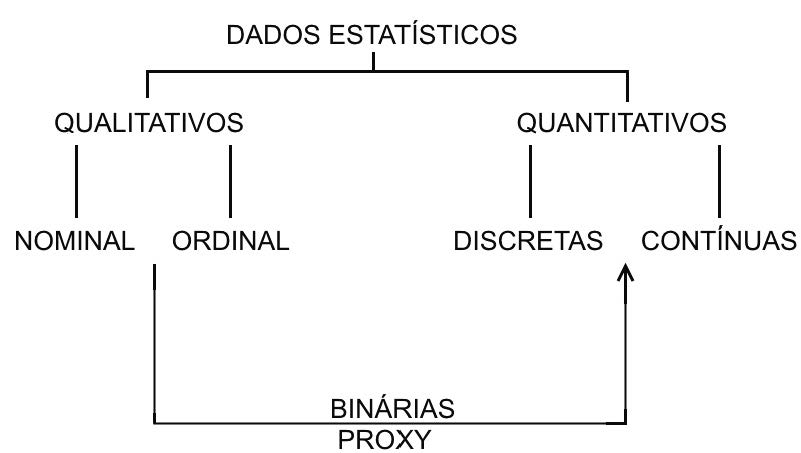
\includegraphics[width=0.75\linewidth]{images2/tipos_variaveis} 

}

\caption{Tipos e codificações de variáveis }\label{fig:unnamed-chunk-25}
\end{figure}

\hypertarget{nouxe7uxf5es-buxe1sicas-sobre-somatuxf3rios-sigma}{%
\section{\texorpdfstring{Noções básicas sobre somatórios (\(\Sigma\))\}}{Noções básicas sobre somatórios (\textbackslash Sigma)\}}}\label{nouxe7uxf5es-buxe1sicas-sobre-somatuxf3rios-sigma}}

Somatório é um operador matemático utilizado para simplificar expressões que envolvam soma de mais de um elemento.

Digamos, por exemplo, que estamos interessados saber o total de comissões a pagar em um determinado setor de uma empresa.

Admita que esse setor tenha 6 funcionários: Pedro, Guilherme, Lucas, Maria, Fernanda e Roberto e que suas comissões sejam R\$ 3000; R\$ 3300; R\$ 3900; R\$ 2950; R\$ 3150 e R\$ 3450.

A representação da soma das comissões pode ser expressa de vários modos como, por exemplo, nesse extensa frase:

\hfill\break

\begin{quote}
O total de comissões a pagar em um determinado setor de uma empresa é a Renda do Pedro mais a Renda do Guilherme mais a Renda do Lucas mais a Renda da Maria mais a Renda da Fernanda mais Renda do Roberto.
\end{quote}

\hfill\break

Atribuindo os valores para cada uma das rendas:

\hfill\break

\begin{quote}
O total de comissões a pagar em um determinado setor de uma empresa é: : R\$ 3000 + R\$ 3300 + R\$ 3900 + R\$ 2950 + R\$ 3150 + R\$ 3450.
\end{quote}

\hfill\break

Chamando-se ``O total de comissões a pagar em um determinado setor de uma empresa é'' de \(X\), teremos:

\hfill\break

\begin{quote}
\(X\) = R\$ 3000 + R\$ 3300 + R\$ 3900 + R\$ 2950 + R\$ 3150 + R\$ 3450.
\end{quote}

\hfill\break

Para simplificar a representação dessa operação, vamos enumerar os funcionários: Pedro (1), Guilherme (2), Lucas (3), Maria (4), Fernanda (5) e Roberto (6). Além disso, vamos chamar a comissão a ser paga pela letra X.

Para diferenciar a fração da comissão \(X\) a ser paga a cada um dos funcionários podemos por um índice na letra \(X\) para indicar a quem estamos nos referindo. Assim \(X_{1}\) seria a comissão do Pedro, \(X_{2}\) a do Guilherme, \(X_{3}\) a do Lucas, \(X_{4}\) a da Maria, \(X_{5}\) a da Fernanda e \(X_{3}\) a do Roberto.

Com essa notação podemos representar matematicamente o total das comissões a pagar em um determinado setor de uma empresa por:

\begin{quote}
\(X=X_{1}+X_{2}+X_{3}+X_{4}+X_{5}+X_{6}\)
\end{quote}

Cada um desses fatores pode ser generalizado como um \(X_{i}\), a comissão de um \emph{i-ésimo} funcionário qualquer. Sabendo que o setor tem apenas 6 funcionários (Pedro, Guilherme, Lucas, Maria, Fernanda e Roberto) então esse i irá variar de 1 a 6 (Pedro:1, Guilherme: 2, Lucas: 3, Maria: 4, Fernanda: 5 e Roberto: 6).

Com todas essas considerações podemos representar a soma das comissões utilizando a notação matemática do somatório.

A letra grega maiúscula \textbf{\(\Sigma\) (sigma)} é habitualmente adotada na matemática para representar o somatório de uma quantidade de fatores. Assim, nosso exemplo da soma de 6 fatores (comissões) pode ser representada matematicamente por:

\[
\sum_{i=1}^{6}{X_{i}} = X_{1}+X_{2}+X_{3}+X_{4}+X_{5}+X_{6}
\]

Observe que abaixo da letra \(\Sigma\) vemos \(i=1\) indicando que o índice dos fatores (X) a serem somados (a \emph{i-ésima} comissão) irá se iniciar pela comissão do primeiro funcionário, quando então i = 1.

Acima da letra \(\Sigma\) vemos o número \(6\) indicando que o índice dos fatores (X) a serem somados irá se dar até o valor da comissão do sexto funcionário, quando então i=6.

Generalizando-se para uma soma de \(n\) fatores \(X\):

\[
\sum_{i=1}^n{X_{i}}.
\]

A representação matemática do somatório pode ser inserida junto a qualquer outra operação como, por exemplo, podemos, depois de realizar a soma, dividi-la por um valor \(n\) qualquer

\[
\frac{\sum_{i=1}^n{X_{i}}}{n} \\
\]

ou elevá-la ao quadrado:

\[
\left(\sum_{i=1}^n{X_{i}}\right)^{2}
\]

Atenção para a diferença entre essas duas operações:

\[
\left(\sum_{i=1}^n{X_{i}}\right)^{2}   \\
\sum_{i=1}^n{X_{i}^{2}}
\]

A primeira indica que devemos realizar a soma dos fatores \textbf{e só então elevar esse resultado ao quadrado}. A segunda indica que devemos realizar a \textbf{soma dos quadrados de cada um dos fatores}.

\hypertarget{anuxe1lise-combinatuxf3ria-diagramas-de-uxe1rvore-permutauxe7uxf5es-arranjos-combinauxe7uxf5es}{%
\section{Análise combinatória: diagramas de árvore, permutações (arranjos) \& combinações}\label{anuxe1lise-combinatuxf3ria-diagramas-de-uxe1rvore-permutauxe7uxf5es-arranjos-combinauxe7uxf5es}}

\hfill\break

A análise combinatória é um conjunto de técnicas para agrupamento de objetos conforme regras definidas e obtenção, através de cálculos, do número de agrupamentos possíveis.

\hfill\break

Se um evento \(E\) pode ser decomposto em eventos sequenciais \(E_{1}\), \(E_{2}\), \(E_{2}\), \ldots, \(E_{n}\) e existem \(P_{1}\) possibilidades distintas de ocorrer \(E_{1}\), \(P_{2}\) possibilidades distintas de ocorrer \(E_{2}\) e assim sucessivamente, então o número total de possibilidades do evento \(E\) ocorrer é dado por:

\hfill\break

\[
P_{1}.P_{2}. \hspace{0.5cm}... \hspace{0.5cm}.P_{n}
\]\\

Esse princípio recebe o nome de \emph{Princípio multiplicativo}, e é aplicado nos casos em que os eventos são interligados pelo conectivo \textbf{e}, característico de decisões sucessivas.

\hfill\break

Se um homem tem 2 camisas e 4 gravatas, então ele tem \(2 \times 4 = 8\) formas de combinar uma camisa com uma gravata.

\hfill\break

Um diagrama como ilustrado na Figura \ref{fig:fig12} (denominado \textbf{diagrama de árvore} em virtude de sua aparência) geralmente é usado para explicar o princípio acima

\hfill\break

\begin{figure}

{\centering 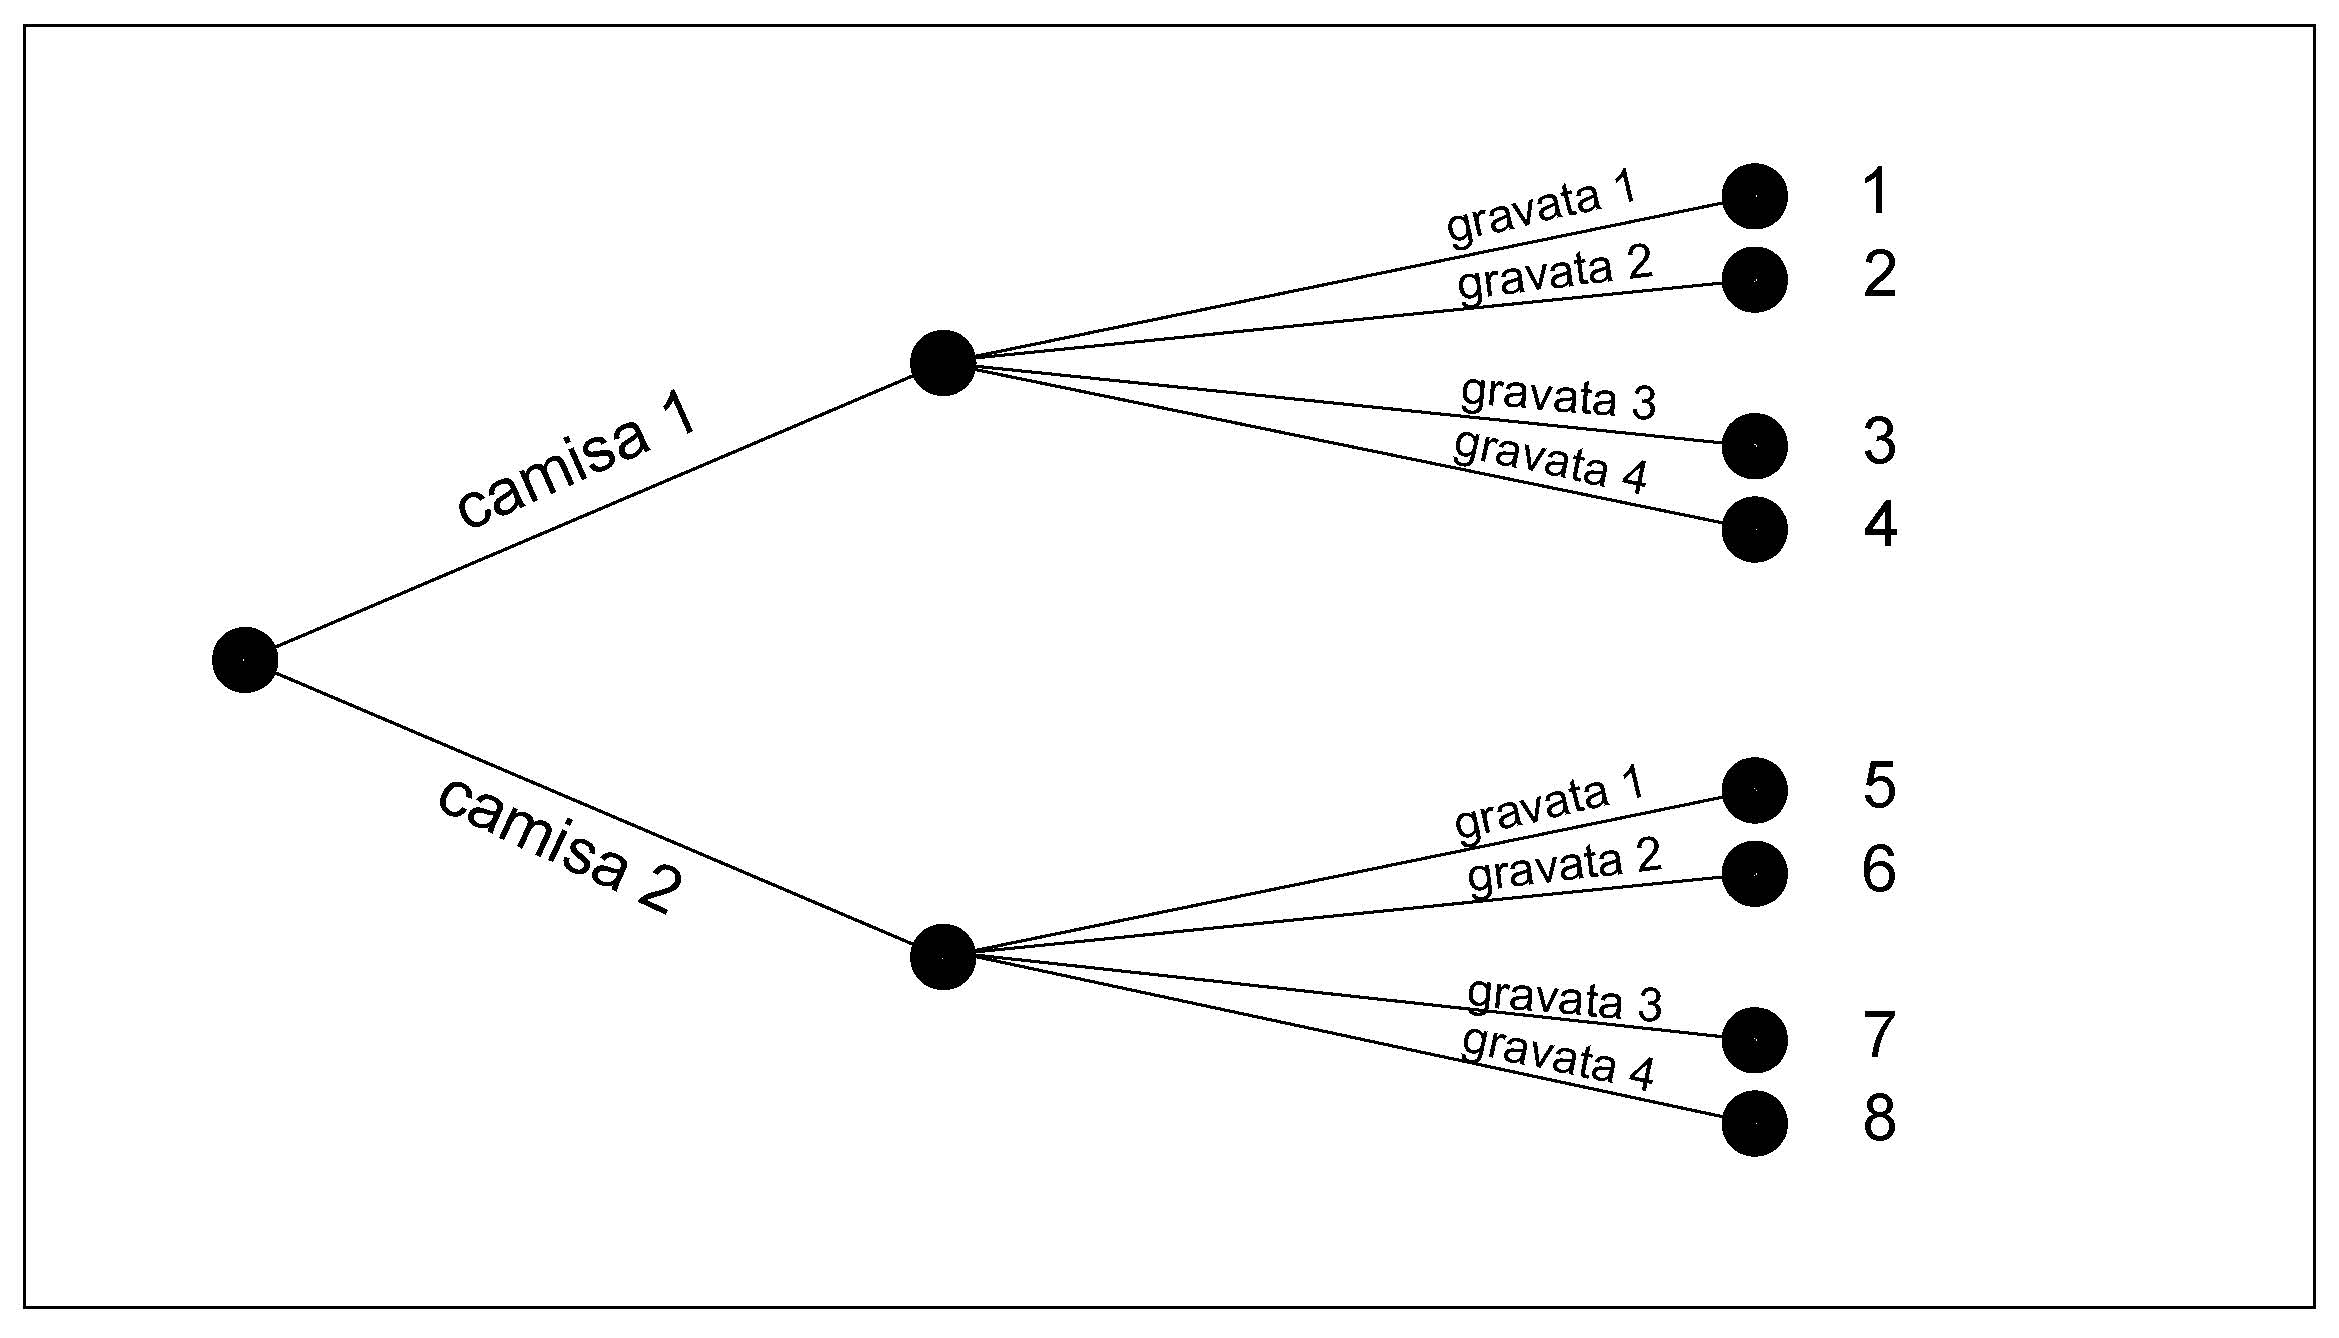
\includegraphics[width=0.5\linewidth]{images4/diagrama_arvore} 

}

\caption{Diagrama de árvore}\label{fig:fig12}
\end{figure}

\hfill\break

Ao lançarmos uma moeda três vezes (assumindo-se que K: cara e C: coroa) haverá \(2 \times 2 \times 2 = 8\) possibilidades distintas.

\hfill\break

O \textbf{diagrama de árvore} associado será (cf.~Figura \ref{fig:fig13}:

\hfill\break

\begin{figure}

{\centering 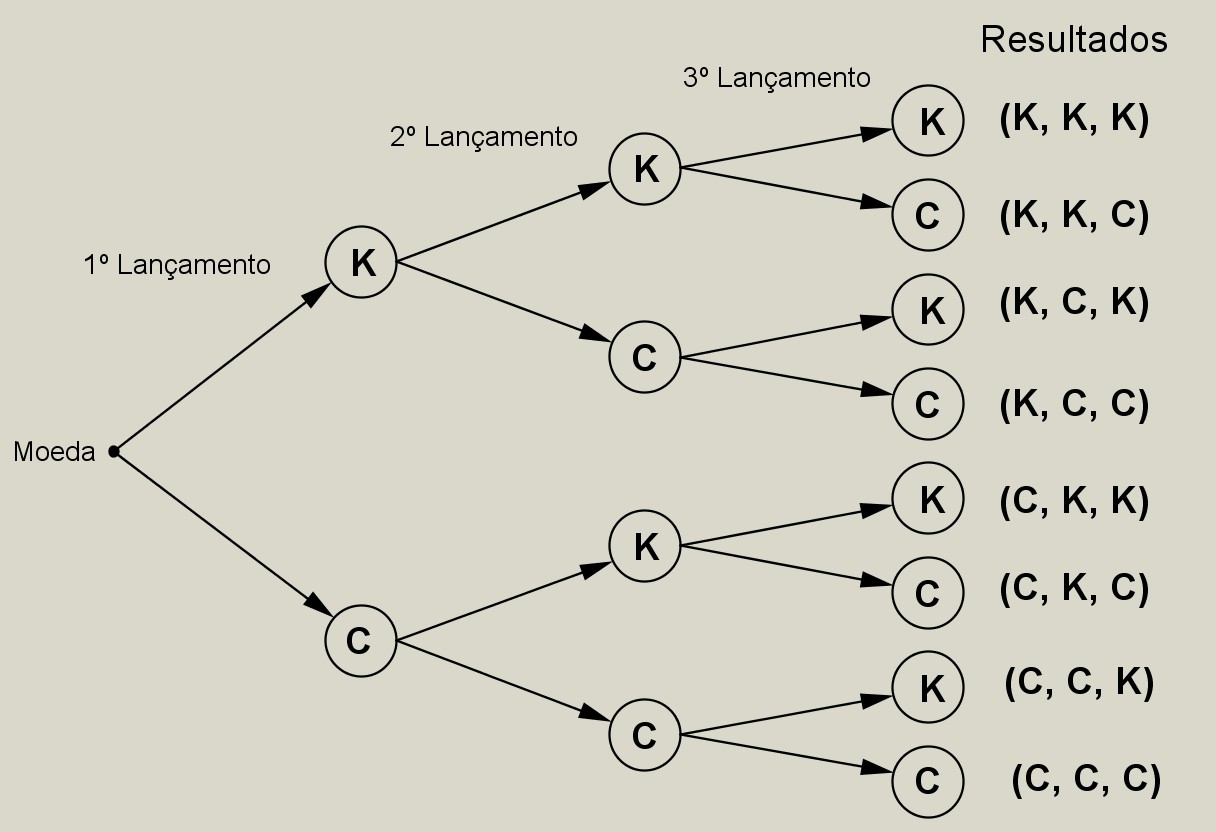
\includegraphics[width=0.5\linewidth]{images4/diagrama_arvore_moeda} 

}

\caption{Diagrama de árvore}\label{fig:fig13}
\end{figure}

\hfill\break

Sejam os eventos mutuamente exclusivos \(E_{1}\) com \(n{1}\) possibilidades distintas de ocorrer, \(E_{2}\) com \(n_{2}\), \ldots, \(E_{n}\) com \(n_{k}\); então o número total de possibilidades de ocorrer \textbf{pelo menos um desses eventos} será dado por:

\[
n_{2} + n_{2} + ... + n_{k}
\]

\hfill\break

Esse princípio recebe o nome de \emph{Princípio aditivo}, e é aplicado nos casos em que os eventos são interligados pelo conectivo \textbf{ou}, característico de eventos mutuamente exclusivos.

\hfill\break

Uma cantina de um colégio possui três tipos de sucos e dois tipos de refrigerantes. Um aluno pode adquirir apenas 1 suco ou 1 refrigerante. Quantas possibilidades de escolha ele tem?

\hfill\break

Seja \(E_{1}\) definido como escolher um tipo de suco (\(n_{1}=3\)) e \(E_{2}\) definido como escolher 1 tipo de refrigerante (\(n_{2}=2\). Então o número total de possíveis escolhas será dado aplicando-se o princípio aditivo:

\hfill\break

\[
n_{1} + n_{2}=5
\]

\hfill\break

\hypertarget{permutauxe7uxf5es-ou-arranjos}{%
\subsection{Permutações ou arranjos}\label{permutauxe7uxf5es-ou-arranjos}}

~

O conceito de uma permutação (arranjo) refere-se a uma relação de \(n\) objetos distintos que serão agrupados \(p\) ~\(p\) (\(p < n\)). Nos agrupamentos possíveis considera-se a ordem dos elementos; sendo assim, qualquer mudança na ordem dos elementos em um agrupamento constitui um novo agrupamento: \textbf{agrupamentos que possuem os mesmos objetos em ordem distinta são considerados agrupamentos distintos}.

\hfill\break

\begin{itemize}
\tightlist
\item
  Simples: não ocorre a repetição de um elemento no agrupamento; e,\\
\item
  Com repetição: os elementos que compõem o conjunto podem aparecer repetidos; ou seja, um agrupamento pode apresentar elementos iguais.
\end{itemize}

\hfill\break

O número de permutações (arranjos) \textbf{sem a repetição} de um mesmo elemento no agrupamento, formados por \(p\) elementos selecionados de um conjunto de \emph{n} objetos distintos será:

\[
P_{(n,p)} =  \frac{n!}{(n-p)!}
\]

\hfill\break

\begin{quote}
Exemplo: Quantos agrupamentos diferentes (onde a ordem dos elementos é razão para distinção: \emph{permutações}) formados por \textbf{3 letras cada} podem ser formados com as \textbf{7 letras}: A, B, C, D, E, F, G \textbf{sem repetição}?
\end{quote}

\hfill\break

\begin{align*}
n  & = 7 \\
p  & = 3 \\
P_{(n,p)} & = \frac{7!}{ (7-3)!} \\
          & = \frac{7!}{4!} = \\
          & = \frac{ 7 \times 6 \times 5 \times 4! }{4!}  \\
          & = 7 \times 6 \times 5  = 210   
\end{align*}

\hfill\break

O número de permutações (arranjos) \textbf{com repetição} de um mesmo elemento no agrupamento, formados por \(p\) elementos selecionados de um conjunto de \(n\) objetos distintos será:

\[
P_{(n,p)} =  n ^{p}
\]

\hfill\break

\begin{quote}
Exemplo: Quantos agrupamentos diferentes (onde a ordem dos elementos é razão para distinção: \textbf{permutações}) formados por \textbf{3 letras cada} podem ser formados com as \textbf{7 letras}: A, B, C, D, E, F, G \textbf{com repetição}?
\end{quote}

\hfill\break

\begin{align*}
n   &  = 7 \\
p   &  = 3 \\
P_{(n,p)} &  = n^{p} \\
          &   = 7 ^{3} = 343
\end{align*}

\hfill\break

\hypertarget{combinauxe7uxf5es}{%
\subsection{Combinações}\label{combinauxe7uxf5es}}

Em uma \emph{permutação} consideramos que a \textbf{ordem* que os objetos assumem nos agrupamentos os tornam diferentes uns dos outros. Por exemplo, }abc** é uma agrupamento distinto de \textbf{bca} numa permutação.

\hfill\break

Em muitos problemas, entretanto, estamos interessados somente na seleção ou escolha dos objetos **sem que a ordem assumida pelos objetos nos agrupamentos os tornem diferentes uns dos outros*.

\hfill\break

Tais seleções são chamadas de \emph{combinações}. Por exemplo, \textbf{abc} e \textbf{bca} são consideradas uma mesma combinação.

\hfill\break

O conceito de uma combinação refere-se a uma relação de \(n\) objetos distintos que serão agrupados \(p\) a \(p\) (\(p < n\)) sem repetição de qualquer objeto em um mesmo agrupamento. Os agrupamentos que possuem os mesmos objetos em ordem diferente \textbf{não são considerados agrupamentos distintos}.

\hfill\break

\begin{itemize}
\tightlist
\item
  Simples: não ocorre a repetição de elementos no agrupamento; e,\\
\item
  Com repetição: os elementos que compõem o agrupamento podem aparecer repetidos; ou seja, ocorre a repetição de um mesmo elemento em um agrupamento.
\end{itemize}

\hfill\break

O número total de combinações sem repetição, de \(p\) objetos selecionados de \(n\) (também chamado de combinações de \(n\) elementos tomados \(p\) a cada vez) é representado por:

\hfill\break
\[
C_{(n,p)} = \frac{ n! }{ p! \times ( n-p)!} 
\]

\hfill\break

\begin{quote}
Exemplo: Qual é número de formas nas quais \(3\) cartas podem ser escolhidas ou selecionadas de um total de \(8\) cartas diferentes?
\end{quote}

\hfill\break

\begin{align*}
n & = 8 \\
p & = 3 \\
C_{(n,p)} & = \frac{8!}{ 3! (8-3)!}  \\
          & = \frac{8!}{3! \times 5!} \\
          & = \frac{ 8 \times 7 \times 6 \times 5! }{ 3! \times 5! } \\
          & = \frac{ 8 \times 7 \times 6 }{3!} = 56  
\end{align*}

\hfill\break

O número total de combinações com repetição, de \(p\) objetos selecionados de \(n\) (também chamado de combinações de \(n\) elementos tomados \(p\) a cada vez com repetição) é representado por:

\hfill\break

\[
C_{(n+p-1,p)} = \frac{ (n+p-1)! }{ p! \times ( n-1)!}
\]

\hfill\break

\begin{quote}
Exemplo: Supondo que você queira comprar um sorvete com 4 bolas em uma sorveteria que possui 3 sabores disponíveis: chocolate, baunilha e morango. De quantos modos diferentes você pode fazer esta compra? (Note que nesta combinação é possível repetir a ordem de dois ou mais sabores, assim tratando de uma combinação com repetição).
\end{quote}

\hfill\break

\begin{align*}
n & =  3 \\
p & = 4 \\ 
C_{(n+p-1,p)} & = \frac{(3+4-1)!}{ 4! (+3-1)!} = 15  
\end{align*}

\hfill\break

\hypertarget{observauxe7uxf5es-acerca-de-alguns-fatoriais}{%
\subsection{Observações acerca de alguns fatoriais}\label{observauxe7uxf5es-acerca-de-alguns-fatoriais}}

~

\begin{align*}
P_{(n,n)} & = \frac{n!}{(n-n)!} = \frac{n!}{0!} = n! \\
C_{(n,0)} & = \frac{n!}{ 0! \times (n-0)! } = \frac{n!}{ 1 \times (n)!} = 1 \\
C_{(n,1)} & = \frac{n! }{ 1! (n-1)!} \\
   & = \frac{ n! }{(n-1)! } \\
   & = \frac{ n \times (n-1)! }{ (n-1)!} = n    
\end{align*}

\hypertarget{conectivos-luxf3gicos}{%
\section{Conectivos lógicos}\label{conectivos-luxf3gicos}}

Muitos dos problemas ligados à probabilidade de ocorrência de eventos são propostos com o auxílio de conectivos lógicos:

\hfill\break

\begin{itemize}
\tightlist
\item
  \textbf{Proposição}: a afirmação de que algo é verdadeiro. Após analisarmos qualquer proposição, podemos defini-la como verdadeira ou falsa como, por exemplo: ``o céu é azul'';
\item
  \textbf{Negação}: negação do valor lógico de uma proposição. A negação de uma proposição verdadeira é falsa. A negação de uma proposição falsa é verdadeira. Os símbolos da negação são o til \(^{-}\) ou \(^{c}\);
\item
  \textbf{Conjunção}: proposição composta com a utilização do conectivo ``e'' como, por exemplo: ``o céu é azul e as nuvens são brancas''. Os símbolos usuais para uma conjunção são: \(\cap\) ou a letra ``V'' invertida; e,
\item
  \textbf{Disjunção}: proposição composta com a utilização do conectivo ``ou'' como, por exemplo, ``o céu é azul ou os pássaros são pretos''. Os símbolos usuais para uma disjunção são: \(\cup\) ou a letra \(V\).
\end{itemize}

\hypertarget{leis-de-de-morgan}{%
\section{Leis de De Morgan}\label{leis-de-de-morgan}}

Augustus de Morgan foi um matemático e lógico indiano.

\hfill\break

\begin{figure}

{\centering 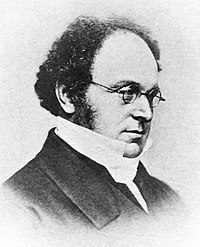
\includegraphics[width=0.5\linewidth]{images4/de_morgan} 

}

\caption{Augustus De Morgan (1806 - 1871)}\label{fig:unnamed-chunk-26}
\end{figure}

\hfill\break

Primeira Lei de De Morgan:

\hfill\break

Negar duas proposições ligadas com ``e'' (\(\cap\)); ou seja, uma \textbf{conjunção}, é o mesmo que negar duas proposições e ligá-las com ``ou''' (ou seja, transformá-las em uma disjunção). Considerando as proposições ``p'' e ``q'' teremos:

\hfill\break

\begin{itemize}
\tightlist
\item
  \(\sim (p \cap q) = (~p) \cup (~q)\); ou,\\
\item
  \((p \cap q)^{c} = (p^{c}) \cup (q^{c})\).
\end{itemize}

\hfill\break

Segunda Lei de De Morgan:

\hfill\break

Negar duas proposições ligadas por ``ou''' (\(\cup\)); ou seja, uma \textbf{disjunção}, é o mesmo que negar as duas proposições e ligá-las com ``e'' (ou seja, transformá-las em uma conjunção). Considerando as proposições ``p'' e ``q'' teremos:

\hfill\break

\begin{itemize}
\tightlist
\item
  \(\sim (p \cup q) = (~p) \cap (~q)\); ou,\\
\item
  \((p \cup q)^{c}= (p^{c}) \cap (q^{c})\).
\end{itemize}

\hypertarget{nouxe7uxf5es-buxe1sicas-para-o-uso-de-calculadora-cassio-fx-82ms}{%
\section{Noções básicas para o uso de calculadora (Cassio fx-82MS)}\label{nouxe7uxf5es-buxe1sicas-para-o-uso-de-calculadora-cassio-fx-82ms}}

Em estatística trabalha-se muito com a análise de um ou mais conjuntos de dados, sendo comum a realização de diversas operações matemáticas com esses dados. Muitas dessas operações envolvem somatórios, por exemplo, e para simplificar essas operações o uso da calculadora se torna essencial.

Neste curso recomenda-se o uso de uma calculadora científica. Existem diversas calculadoras que cumprem as funções necessárias nesse curso. Para padronizar as aulas, alguns professores sugerem a calculadora científica de código: FX82MS, que é a calculadora que cujo funcionamento será exibido a seguir, passo a passo. A seguir serão descritas algumas das funções básicas mais importantes no uso desta calculadora.

Primeiro vamos deixar a calculadora no modo de regressão linear. Esse modo permite que a calculadora
funcione normalmente para as operações comuns (soma, subtração, multiplicação e divisão), e ainda libera
todas as funções importantes nesse curso. Sempre que o aluno for utilizar a calculadora, ele deve se certificar que ela esteja no modo de regressão linear, da seguinte forma:

PASSO 1:

\begin{itemize}
\item
  \begin{enumerate}
  \def\labelenumi{\arabic{enumi}.}
  \tightlist
  \item
    ON
  \end{enumerate}
\item
  \begin{enumerate}
  \def\labelenumi{\arabic{enumi}.}
  \setcounter{enumi}{1}
  \tightlist
  \item
    MODE
  \end{enumerate}
\item
  \begin{enumerate}
  \def\labelenumi{\arabic{enumi}.}
  \setcounter{enumi}{2}
  \tightlist
  \item
    Aperte 3 para escolher REG
  \end{enumerate}
\item
  \begin{enumerate}
  \def\labelenumi{\arabic{enumi}.}
  \setcounter{enumi}{3}
  \tightlist
  \item
    Aperte 1 para escolher LIN
  \end{enumerate}
\end{itemize}

Repare que no topo do visor da calculadora apareceu o símbolo \textcolor{red}{REG}, que indica que a calculadora está em modo de regressão. Desde que esteja no modo de regressão, podemos passar para o passo seguinte.

O nosso objetivo aqui é inserir o conjunto de dados na calculadora para então realizarmos as operações necessárias. Mas antes de inserir os dados, temos que garantir que a calculadora esteja \textcolor{red}{vazia} para o novo conjunto de dados. Ou seja, devemos limpar a calculadora:

PASSO 2:

\begin{itemize}
\item
  \begin{enumerate}
  \def\labelenumi{\arabic{enumi}.}
  \tightlist
  \item
    SHIFT
  \end{enumerate}
\item
  \begin{enumerate}
  \def\labelenumi{\arabic{enumi}.}
  \setcounter{enumi}{1}
  \tightlist
  \item
    MODE
  \end{enumerate}
\item
  \begin{enumerate}
  \def\labelenumi{\arabic{enumi}.}
  \setcounter{enumi}{2}
  \tightlist
  \item
    Aperte 1 para escolher Scl ( \emph{Stat Clear})
  \end{enumerate}
\item
  \begin{enumerate}
  \def\labelenumi{\arabic{enumi}.}
  \setcounter{enumi}{3}
  \tightlist
  \item
    Aperte = para limpar a calculadora
  \end{enumerate}
\end{itemize}

Entrada de dados.

Agora que a calculadora está em modo de regressão e está limpa, podemos inserir o conjunto de dados. Para ilustrar esta função, vamos inserir o seguinte conjunto de dados: \(X= {5,3,6,2}\).

Para inserir cada um desses elementos você deve digitar o número e em seguida o botão M+.

A sequência fica assim: 5 M+ 3 M+ 6 M+ 2 M+.

A cada vez que você insere uma observação, a calculadora atualiza o número de observações inseridas. No final, nesse caso, aparece \textcolor{red}{n=4} porque inserimos 4 observações.

Funções envolvendo somatórios.

Observe na calculadora os botões \textcolor{orange}{shift} e \textcolor{red}{alpha}. Geralmente estes botões aparecem nas cores amarela e vermelha, respectivamente. Observe ainda que alguns botões da calculadora possuem termos nessas cores. Para selecionar as funções em \textcolor{orange}{amarelo}, antes devemos ligar o modo \textcolor{orange}{shift}. Enquanto que para selecionar as funções em \textcolor{red}{vermelho} deve-se ligar o modo \textcolor{red}{alpha}.

Por exemplo, para abrir a função \textcolor{orange}{S-SUM} que está em \textcolor{orange}{amarelo} no botão 1, faz-se: SHIFT 1. A função \textcolor{orange}{S-SUM} é a que contém todos os somatórios importantes. Ao abrir esta função aparecem três opções da seguinte forma:

\[
\Sigma(x) \\
\Sigma(x^{2})\\
n 
\]

Aperta-se 1 = para ter o somatório de \(x\); 2 = para ter o somatório de \(x^{2}\) ou 3 = para saber o número \(n\) de obervações inseridas.

Funções para obter a média e o desvio padrão.

A função \textcolor{orange}{S-VAR} fornece a média e o desvio padrão dos dados. Essas são medidas importantes, que serão utilizadas durante todo o curso. Para abrir esta função faz-se: SHIFT 2.

\[
\stackrel{-}{x}
\sigma_{x}
S_{x}
\]

A opção 1 retorna a média dos dados, a opção 2 retorna o desvio padrão populacional e a opção 3 o desvio padrão amostral.

Como inserir dois conjuntos de dados.

Quando se deseja estudar dois conjuntos de dados, de mesmo tamanho, pode-se inseri-los de forma simultânea na calculadora. Para ilustrar vamos inserir os seguintes conjuntos de dados: \(X={2,7,4,3,2}\) e \(Y={1,2,3,6,5}\). \textcolor{red}{Antes de inserir os dados, lembre-se de limpar a calculadora}.

Em seguida vamos inserir os dados de 2 em 2: o primeiro de X com o primeiro de Y e assim por diante. Repare que ao lado do botão M+ tem um botão com uma vírgula. Esta vírgula é utilizada para separar as observações de X das de Y . A sequência fica assim:

\begin{itemize}
\tightlist
\item
  2,1 M+
\item
  7,2 M+
\item
  4,3 M+
\item
  3,6 M+
\item
  2,5 M+
\end{itemize}

Se você usar a função \textcolor{orange}{S-SUM}, na tela vai aparecer os somatórios apenas de X, que foi pela ordem, o primeiro a ser inserido. Na calculadora tem um botão grande e style=``color:gray;''\textgreater S-SUM, com 4 setas. Depois de selecionar a função \textcolor{orange}{amarelo} aperte a seta para frente que aparecerão os somatórios para Y . O mesmo acontece para a função \textcolor{orange}{S-VAR}.

\begin{figure}

{\centering 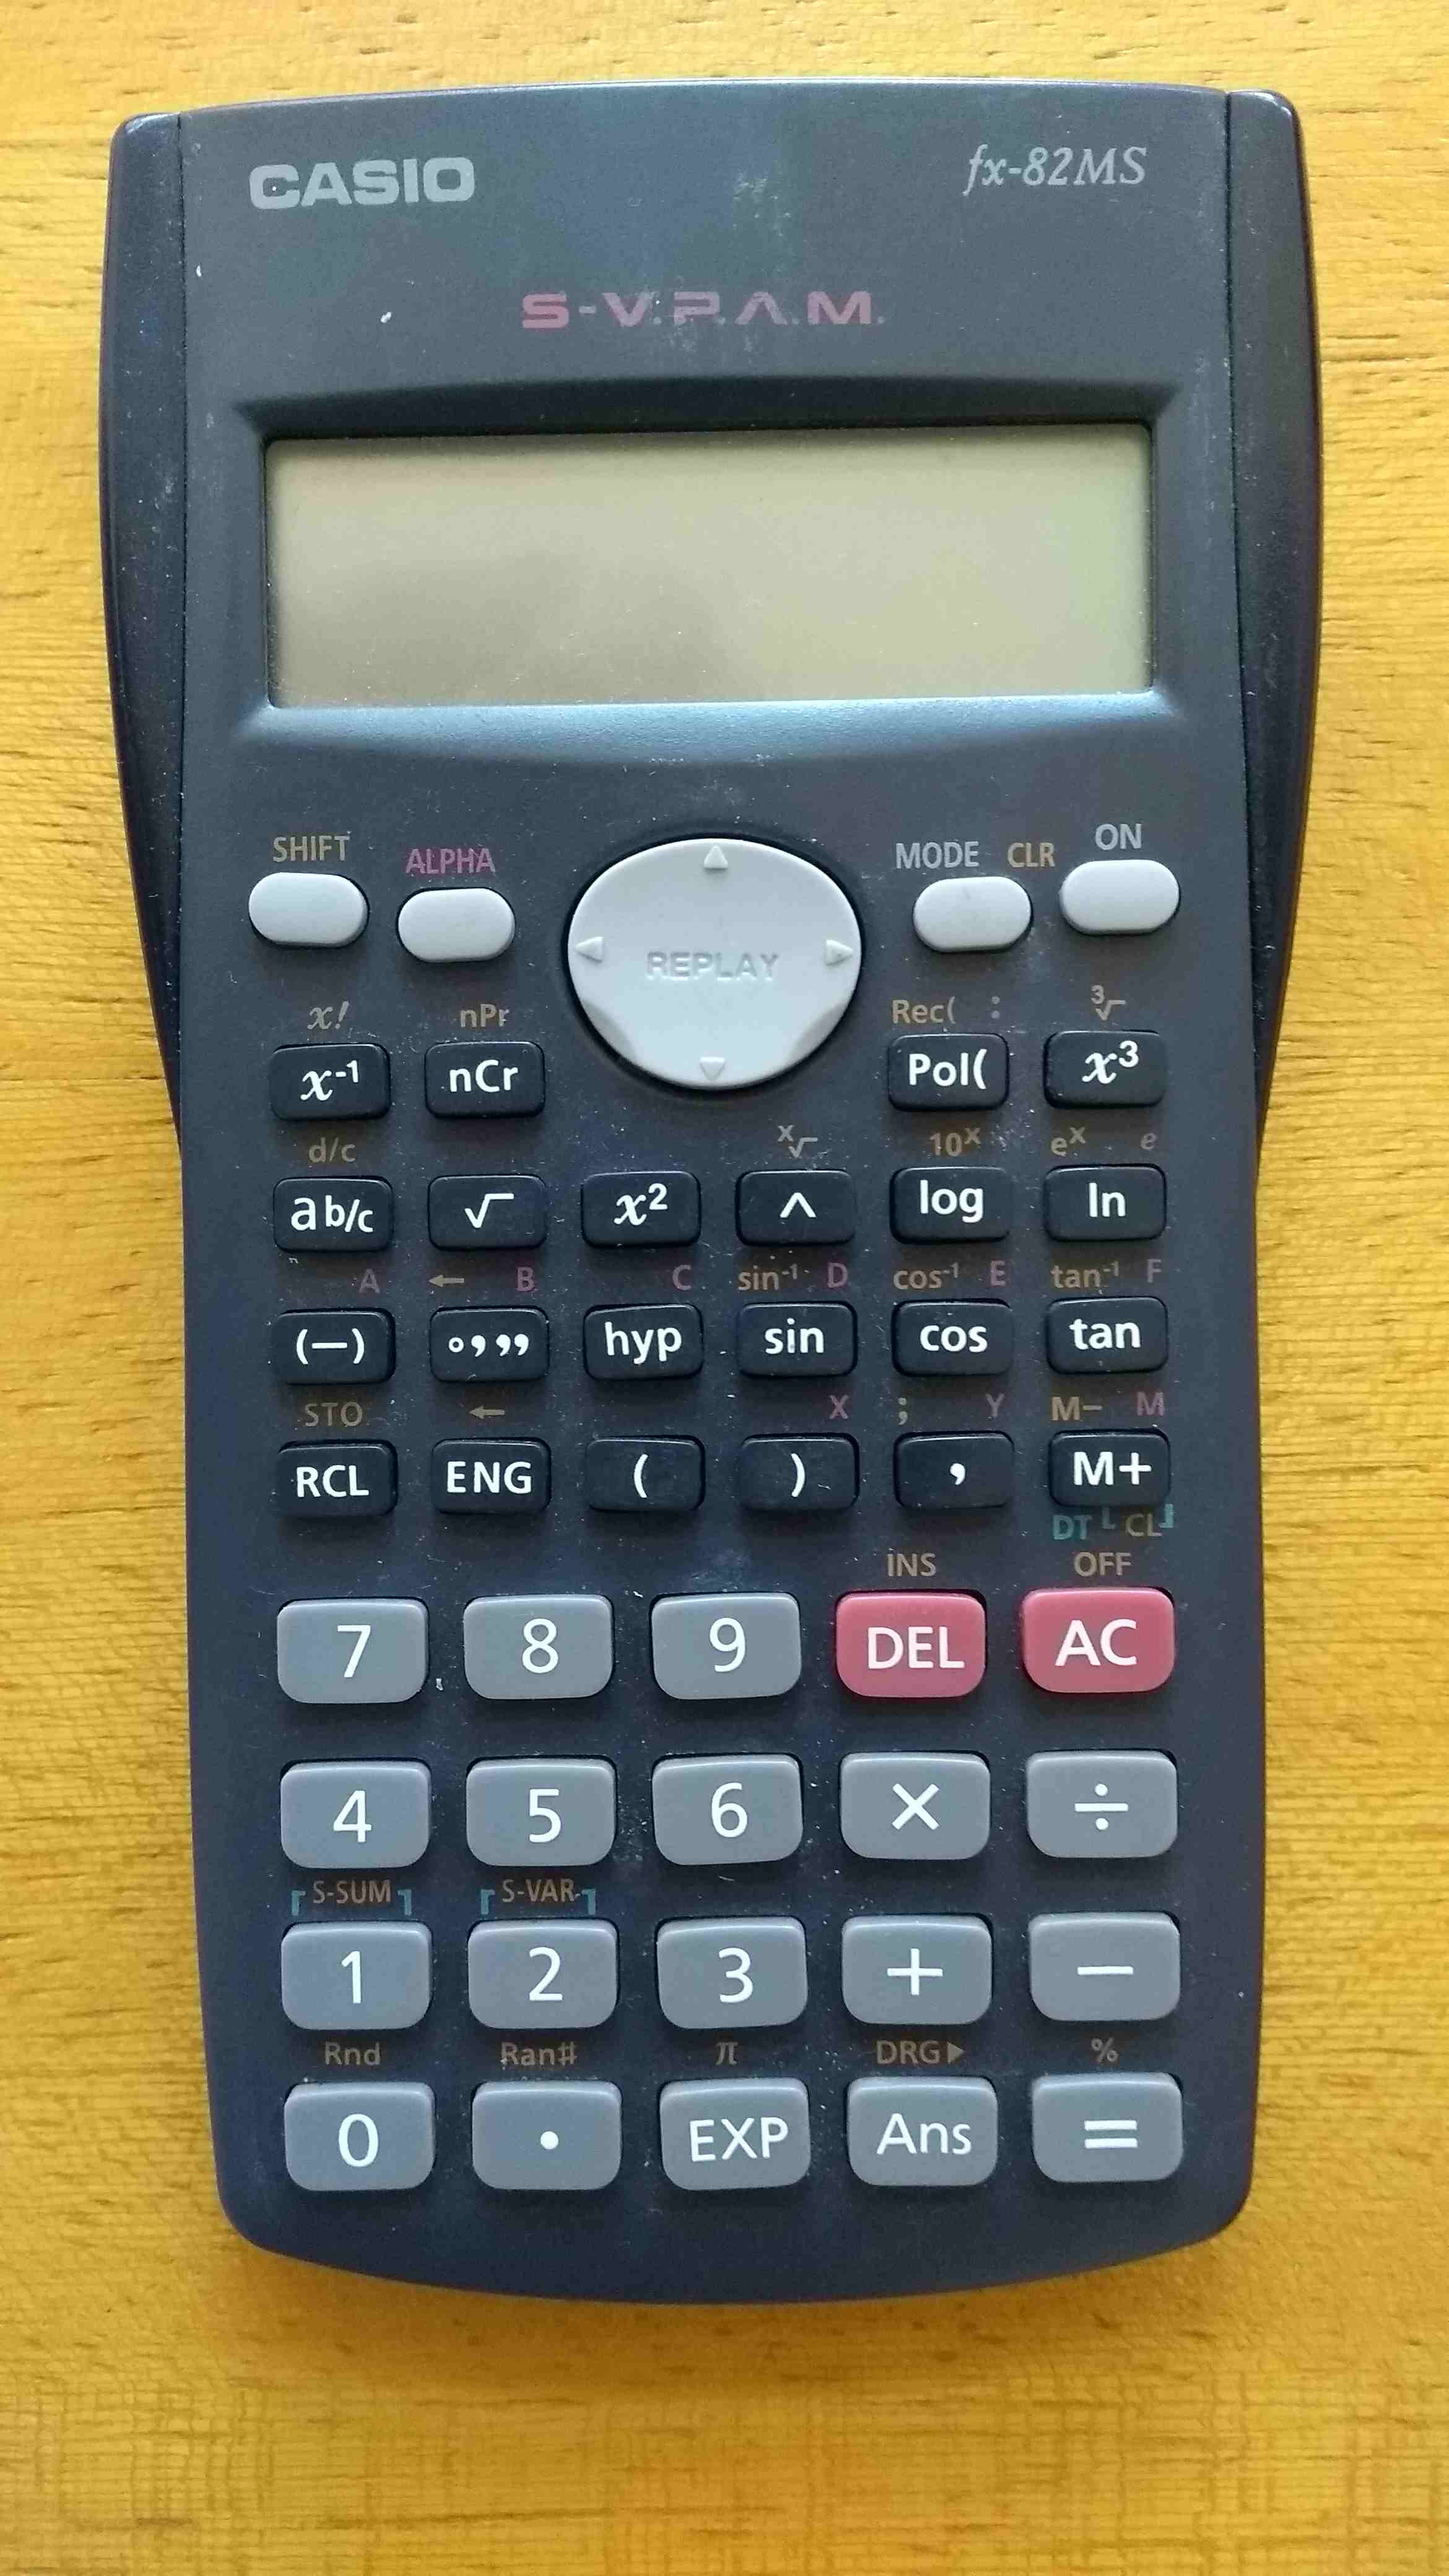
\includegraphics[width=0.8\linewidth]{images2/calculadora_cassio} 

}

\caption{Calculadora Cassio}\label{fig:unnamed-chunk-27}
\end{figure}

\hypertarget{descritiva}{%
\chapter{- Introdução à estatística descritiva}\label{descritiva}}

Do prefácio da tradução do livro de Jack Levin (Estatística aplicada às ciências humanas), Sérgio Francisco Costa diz que o livro:

\begin{quote}
``destina-se a um público muito específico: estudantes de Ciências Humanas, refúgio errôneo dos que fogem das equações e dos cálculos, pois que, embora humanas - e talvez por isso mesmo - não podemos prescindir das tão odiadas quantificações {[}\ldots{]}'\,'
\end{quote}

\hypertarget{anuxe1lise-exploratuxf3ria}{%
\section{Análise exploratória}\label{anuxe1lise-exploratuxf3ria}}

A análise exploratória de dados ( \emph{EDA: Exploratory Data Analisys} , originalmente desenvolvida pelo matemático e estatístico norte-americano John Tukey na década de 1970) é usada para se investigar conjuntos de dados e resumir suas principais características, muitas vezes usando métodos de visualização de dados por gráficos e apresentação de tabelas.

\hfill\break

\begin{figure}

{\centering 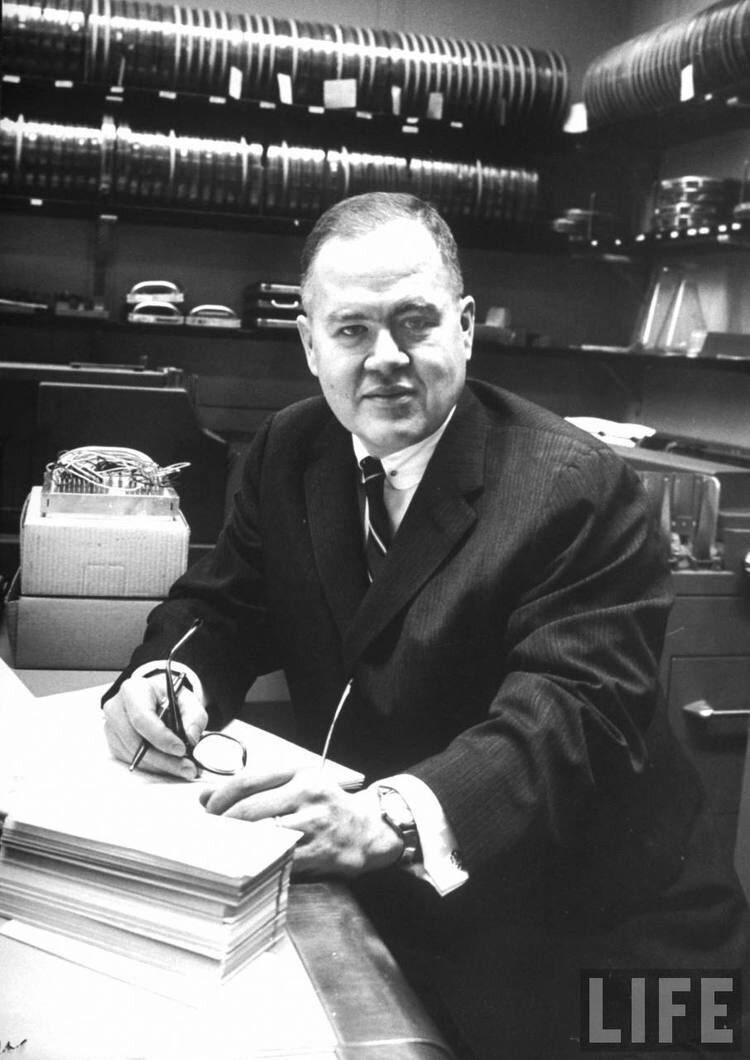
\includegraphics[width=0.5\linewidth]{images3/tukey} 

}

\caption{John Tukey (1915-2000)}\label{fig:unnamed-chunk-29}
\end{figure}

\hfill\break

Habitualmente uma \emph{EDA} envolve:

\begin{itemize}
\tightlist
\item
  verificar quais são os tipos de variáveis presentes nos dados;
\item
  sintetizar os valores assumidos por cada uma das variáveis;
\item
  verificar os padrões de cada variável e eventuais associações entre duas ou mais delas; e,
\item
  apresentação de tabelas e gráficos expositivos variados.
\end{itemize}

\hypertarget{dados-brutos-em-rol-diagrama-de-ramos-folhas-e-de-dispersuxe3o-unidimensional}{%
\section{Dados brutos, em rol, diagrama de ramos \& folhas e de dispersão unidimensional}\label{dados-brutos-em-rol-diagrama-de-ramos-folhas-e-de-dispersuxe3o-unidimensional}}

Consideremos os dados obtidos da medição das alturas em metros de 60 estudantes de uma determinada classe de um certo curso aqui na UEL:

\begin{Shaded}
\begin{Highlighting}[]
\NormalTok{alturas}\OtherTok{=}\FunctionTok{c}\NormalTok{(}\FloatTok{1.63}\NormalTok{,}\FloatTok{1.67}\NormalTok{,}\FloatTok{1.47}\NormalTok{,}\FloatTok{1.64}\NormalTok{,}\FloatTok{1.66}\NormalTok{,}\FloatTok{1.73}\NormalTok{,}\FloatTok{2.00}\NormalTok{,}\FloatTok{1.62}\NormalTok{,}\FloatTok{1.65}\NormalTok{,}\FloatTok{1.56}\NormalTok{,}\FloatTok{1.65}\NormalTok{,}\FloatTok{1.85}\NormalTok{,}\FloatTok{1.73}\NormalTok{,}
          \FloatTok{1.78}\NormalTok{,}\FloatTok{1.82}\NormalTok{,}\FloatTok{1.68}\NormalTok{,}\FloatTok{1.67}\NormalTok{,}\FloatTok{1.83}\NormalTok{,}\FloatTok{1.72}\NormalTok{,}\FloatTok{1.71}\NormalTok{,}\FloatTok{1.73}\NormalTok{,}\FloatTok{1.67}\NormalTok{,}\FloatTok{1.66}\NormalTok{,}\FloatTok{1.95}\NormalTok{,}\FloatTok{1.76}\NormalTok{,}\FloatTok{1.73}\NormalTok{,}
          \FloatTok{1.77}\NormalTok{,}\FloatTok{1.68}\NormalTok{,}\FloatTok{1.65}\NormalTok{,}\FloatTok{1.64}\NormalTok{,}\FloatTok{1.66}\NormalTok{,}\FloatTok{1.68}\NormalTok{,}\FloatTok{1.61}\NormalTok{,}\FloatTok{1.73}\NormalTok{,}\FloatTok{1.72}\NormalTok{,}\FloatTok{1.83}\NormalTok{,}\FloatTok{1.69}\NormalTok{,}\FloatTok{1.84}\NormalTok{,}\FloatTok{1.66}\NormalTok{,}
          \FloatTok{1.78}\NormalTok{,}\FloatTok{1.54}\NormalTok{,}\FloatTok{1.74}\NormalTok{,}\FloatTok{1.56}\NormalTok{,}\FloatTok{1.66}\NormalTok{,}\FloatTok{1.56}\NormalTok{,}\FloatTok{1.62}\NormalTok{,}\FloatTok{1.55}\NormalTok{,}\FloatTok{1.86}\NormalTok{,}\FloatTok{1.44}\NormalTok{,}\FloatTok{1.67}\NormalTok{,}\FloatTok{1.76}\NormalTok{,}\FloatTok{1.79}\NormalTok{,}
          \FloatTok{1.75}\NormalTok{,}\FloatTok{1.41}\NormalTok{,}\FloatTok{1.65}\NormalTok{,}\FloatTok{1.58}\NormalTok{,}\FloatTok{1.93}\NormalTok{,}\FloatTok{1.57}\NormalTok{,}\FloatTok{1.71}\NormalTok{,}\FloatTok{1.58}\NormalTok{)}
\NormalTok{alturas}
\end{Highlighting}
\end{Shaded}

\begin{verbatim}
##  [1] 1.63 1.67 1.47 1.64 1.66 1.73 2.00 1.62 1.65 1.56 1.65 1.85 1.73 1.78 1.82
## [16] 1.68 1.67 1.83 1.72 1.71 1.73 1.67 1.66 1.95 1.76 1.73 1.77 1.68 1.65 1.64
## [31] 1.66 1.68 1.61 1.73 1.72 1.83 1.69 1.84 1.66 1.78 1.54 1.74 1.56 1.66 1.56
## [46] 1.62 1.55 1.86 1.44 1.67 1.76 1.79 1.75 1.41 1.65 1.58 1.93 1.57 1.71 1.58
\end{verbatim}

Esse conjunto de dados certamente contém diversas informações acerca da altura dessas pessoas; todavia, da maneira como estão expostos, a visualização dessas informações fica bastante difícil. Esse modo de apresentação é chamado de dados \emph{brutos}.

Com um pequeno refinamento, como pela simples ordenação desses dados (são medidas numéricas contínuas), algumas informações começam a se destacar:

\begin{Shaded}
\begin{Highlighting}[]
\FunctionTok{sort}\NormalTok{(alturas)}
\end{Highlighting}
\end{Shaded}

\begin{verbatim}
##  [1] 1.41 1.44 1.47 1.54 1.55 1.56 1.56 1.56 1.57 1.58 1.58 1.61 1.62 1.62 1.63
## [16] 1.64 1.64 1.65 1.65 1.65 1.65 1.66 1.66 1.66 1.66 1.66 1.67 1.67 1.67 1.67
## [31] 1.68 1.68 1.68 1.69 1.71 1.71 1.72 1.72 1.73 1.73 1.73 1.73 1.73 1.74 1.75
## [46] 1.76 1.76 1.77 1.78 1.78 1.79 1.82 1.83 1.83 1.84 1.85 1.86 1.93 1.95 2.00
\end{verbatim}

A interpretabilidade das informações trazidas por esses dados começa a ficar mais fácil como, por exemplo, as alturas:

\begin{itemize}
\tightlist
\item
  mínima; e,
\item
  máxima dos estudantes.
\end{itemize}

A uma listagem de valores ordenada (de modo crescente ou decrescente) dá-se o nome de \emph{rol}.

Outra forma de apresentação desses dados é por um \emph{Diagrama de Ramos e Folhas}, uma apresentação híbrida pois ao mesmo tempo que espelha a quantidade de medidas observadas para cada altura, mantém as informações da listagem.

\begin{Shaded}
\begin{Highlighting}[]
\FunctionTok{stem}\NormalTok{(alturas)}
\end{Highlighting}
\end{Shaded}

\begin{verbatim}
## 
##   The decimal point is 1 digit(s) to the left of the |
## 
##   14 | 147
##   15 | 45666788
##   16 | 12234455556666677778889
##   17 | 11223333345667889
##   18 | 233456
##   19 | 35
##   20 | 0
\end{verbatim}

À esquerda do traço vertical (os ramos) são apresentadas frações das medidas das alturas (no caso, decímetros) e à direita (as folhas) são apresentadas os complementos dessas medidas (os centímetros) de tal modo que cada um dos dados da amostral original possa ter sua medida resgatada fazendo-se a leitura dos valores à esquerda com cada um deles à direita.

Essa apresentação também oferece uma apreciação visual a respeito de como os valores se distribuem.

Um \emph{Gráfico de dispersão unidimensional (stripchart)} expressa visualmente duas informações: a localização de cada uma das medidas e a dispersão dos dados.

\begin{Shaded}
\begin{Highlighting}[]
\FunctionTok{stripchart}\NormalTok{(alturas, }\AttributeTok{method =} \StringTok{"stack"}\NormalTok{, }\AttributeTok{offset=}\DecValTok{1}\NormalTok{,}
           \AttributeTok{pch=}\DecValTok{20}\NormalTok{, }\AttributeTok{at=}\FloatTok{0.5}\NormalTok{,}
           \AttributeTok{main=}\StringTok{"Gráfico de dispersão unidimensional"}\NormalTok{,}
           \AttributeTok{col=}\StringTok{"blue"}\NormalTok{,}\AttributeTok{cex=}\DecValTok{1}\NormalTok{,}
           \AttributeTok{xlab=}\StringTok{"Alturas dos estudantes (m)"}\NormalTok{,}
           \AttributeTok{ylab=}\StringTok{"Quantidades observadas (un)"}\NormalTok{)}
\end{Highlighting}
\end{Shaded}

\begin{figure}

{\centering 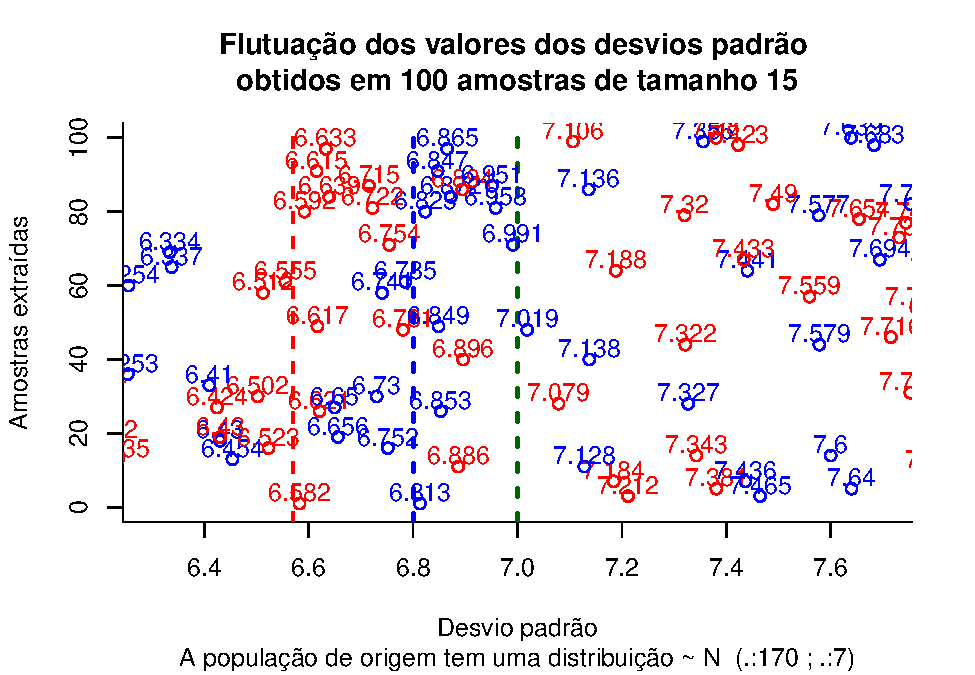
\includegraphics{apostila_files/figure-latex/unnamed-chunk-33-1} 

}

\caption{Gráfico de dispersão unidimensional (stripchart)}\label{fig:unnamed-chunk-33}
\end{figure}

\hypertarget{suxednteses-numuxe9ricas-descritivas}{%
\section{Sínteses numéricas descritivas}\label{suxednteses-numuxe9ricas-descritivas}}

Além da apresentação elementar de algumas informações relacionadas aos dados brutos da amostra, tais como os valores \emph{mínimo} e \emph{máximo} observados, a estatística descritiva possui muitas outras ferramentas para \emph{condensar} a informação contida nos dados.

São chamadas de \emph{sínteses numéricas}, medidas que condensam variados aspectos relacionados aos valores dos dados. As principais \emph{sínteses numéricas} são:

\begin{itemize}
\tightlist
\item
  de tendência central (posição): média (simples ou aritmética, geométrica, harmônica, anarmônica, quadrática, biquadrática), moda e mediana;
\item
  de dispersão (variabilidade): absolutas (amplitude total, variância e desvio padrão) ou relativas (coeficiente de variação, unidades padronizadas); e,
\item
  de subdivisão (separatrizes, quantis): mediana (50\%), quartis (25\%, 50\%, 75\%), decis (10\%, \ldots.90\%) e percentis (1\%\ldots.99\%).
\end{itemize}

Uma medida de posição ou dispersão é dita \textbf{resistente} quando forem pouco afetadas pela alteração de uma pequena porção dos dados. A mediana é uma medida resistente, já a média e a variância não são.

\hypertarget{medidas-de-tenduxeancia-central-posiuxe7uxe3o}{%
\subsection{Medidas de tendência central (posição)}\label{medidas-de-tenduxeancia-central-posiuxe7uxe3o}}

\hypertarget{muxe9dia}{%
\subsubsection{Média}\label{muxe9dia}}

Sejam \(x_{1}, x_{2}, ..., x_{n}\) os \(n\) valores assumidos pela variável \(X\) (dados brutos). A \emph{média aritmética simples} será dada por:

\[
\stackrel{-}{x}=\frac{\sum _{i=1}^{n}{x}_{i}}{n}
\]

Propriedades da média aritmética:

\begin{itemize}
\tightlist
\item
  somando-se (ou subtraindo-se) cada um dos elementos do conjunto de dados por uma constante arbitrária qualquer \(k\), a média aritmética ficará adicionada (ou subtraída) dessa essa constante \(k\)
\end{itemize}

\begin{Shaded}
\begin{Highlighting}[]
\NormalTok{alturas\_ad}\OtherTok{=}\NormalTok{alturas}\FloatTok{+0.05}

\FunctionTok{par}\NormalTok{(}\AttributeTok{mfrow=}\FunctionTok{c}\NormalTok{(}\DecValTok{1}\NormalTok{,}\DecValTok{2}\NormalTok{))}

\FunctionTok{stripchart}\NormalTok{(alturas,}\AttributeTok{method =} \StringTok{"stack"}\NormalTok{,  }\AttributeTok{at=}\FloatTok{0.5}\NormalTok{, }
\AttributeTok{main=}\StringTok{""}\NormalTok{,}\AttributeTok{pch =} \DecValTok{20}\NormalTok{,}
\AttributeTok{col=}\StringTok{"blue"}\NormalTok{, }\AttributeTok{cex=}\DecValTok{1}\NormalTok{, }\AttributeTok{xlab=}\StringTok{"Alturas originais dos estudantes (m)"}\NormalTok{, }
\AttributeTok{ylab=}\StringTok{"Quantidades observadas (un)"}\NormalTok{)}
\FunctionTok{abline}\NormalTok{(}\AttributeTok{v=}\FunctionTok{mean}\NormalTok{(alturas), }\AttributeTok{col=}\StringTok{"red"}\NormalTok{) }
\FunctionTok{text}\NormalTok{(}\FunctionTok{mean}\NormalTok{(alturas)}\SpecialCharTok{{-}}\FloatTok{0.2}\NormalTok{, }\DecValTok{1}\NormalTok{, }\StringTok{"Média=1,69 m"}\NormalTok{, }\AttributeTok{col =} \StringTok{"red"}\NormalTok{, }\AttributeTok{srt=}\DecValTok{90}\NormalTok{) }

\FunctionTok{stripchart}\NormalTok{(alturas\_ad,}\AttributeTok{method =} \StringTok{"stack"}\NormalTok{,  }\AttributeTok{at=}\FloatTok{0.5}\NormalTok{, }
\AttributeTok{main=}\StringTok{""}\NormalTok{,}\AttributeTok{pch =} \DecValTok{20}\NormalTok{,}
\AttributeTok{col=}\StringTok{"blue"}\NormalTok{, }\AttributeTok{cex=}\DecValTok{1}\NormalTok{, }\AttributeTok{xlab=}\StringTok{"Alt. dos estudantes (m) adic. de 5cm"}\NormalTok{, }
\AttributeTok{ylab=}\StringTok{"Quantidades observadas (un)"}\NormalTok{)}
\FunctionTok{abline}\NormalTok{(}\AttributeTok{v=}\FunctionTok{mean}\NormalTok{(alturas\_ad), }\AttributeTok{col=}\StringTok{"red"}\NormalTok{) }
\FunctionTok{text}\NormalTok{(}\FunctionTok{mean}\NormalTok{(alturas\_ad)}\SpecialCharTok{{-}}\FloatTok{0.2}\NormalTok{, }\DecValTok{1}\NormalTok{, }\StringTok{"Média=1,74 m"}\NormalTok{, }\AttributeTok{col =} \StringTok{"red"}\NormalTok{, }\AttributeTok{srt=}\DecValTok{90}\NormalTok{) }
\end{Highlighting}
\end{Shaded}

\begin{figure}

{\centering 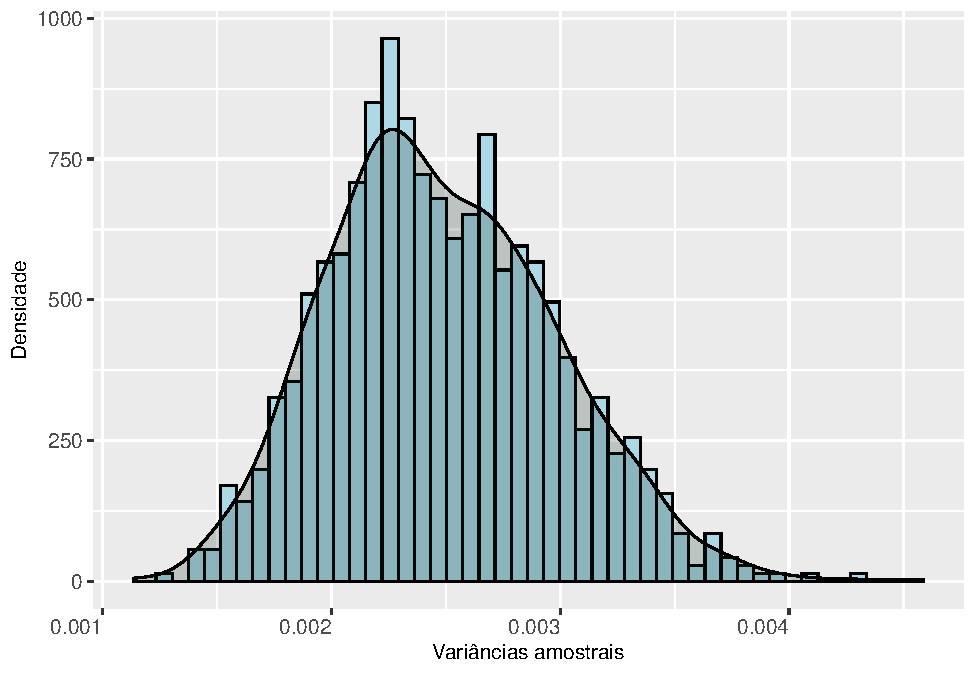
\includegraphics{apostila_files/figure-latex/unnamed-chunk-34-1} 

}

\caption{Mudanças na média pela adição (subtração) de uma constante $k=0.05$}\label{fig:unnamed-chunk-34}
\end{figure}

\begin{itemize}
\tightlist
\item
  multiplicando-se (ou dividindo-se) cada um dos elementos do conjunto de dados por uma constante arbitrária \(k\), a média aritmética ficará multiplicada (ou dividida) por essa constante \(k\)
\end{itemize}

\begin{Shaded}
\begin{Highlighting}[]
\NormalTok{alturas\_mult}\OtherTok{=}\NormalTok{alturas}\SpecialCharTok{*}\FloatTok{1.2}

\FunctionTok{par}\NormalTok{(}\AttributeTok{mfrow=}\FunctionTok{c}\NormalTok{(}\DecValTok{1}\NormalTok{,}\DecValTok{2}\NormalTok{))}

\FunctionTok{stripchart}\NormalTok{(alturas,}\AttributeTok{method =} \StringTok{"stack"}\NormalTok{,  }\AttributeTok{at=}\FloatTok{0.5}\NormalTok{, }
\AttributeTok{main=}\StringTok{""}\NormalTok{,}\AttributeTok{pch =} \DecValTok{20}\NormalTok{,}
\AttributeTok{col=}\StringTok{"blue"}\NormalTok{,  }\AttributeTok{xlab=}\StringTok{"Alturas originais dos estudantes (m)"}\NormalTok{, }
\AttributeTok{ylab=}\StringTok{"Quantidades observadas (un)"}\NormalTok{)}
\FunctionTok{abline}\NormalTok{(}\AttributeTok{v=}\FunctionTok{mean}\NormalTok{(alturas), }\AttributeTok{col=}\StringTok{"red"}\NormalTok{) }
\FunctionTok{text}\NormalTok{(}\FunctionTok{mean}\NormalTok{(alturas)}\SpecialCharTok{{-}}\FloatTok{0.1}\NormalTok{, }\DecValTok{1}\NormalTok{, }\StringTok{"Média=1,69 m"}\NormalTok{, }\AttributeTok{col =} \StringTok{"red"}\NormalTok{, }\AttributeTok{srt=}\DecValTok{90}\NormalTok{) }


\FunctionTok{stripchart}\NormalTok{(alturas\_mult,}\AttributeTok{method =} \StringTok{"stack"}\NormalTok{,  }\AttributeTok{at=}\FloatTok{0.5}\NormalTok{, }
\AttributeTok{main=}\StringTok{""}\NormalTok{,}\AttributeTok{pch =} \DecValTok{20}\NormalTok{,}
\AttributeTok{col=}\StringTok{"blue"}\NormalTok{,  }\AttributeTok{xlab=}\StringTok{"Alt. dos estudantes (m) mult. por 1,2"}\NormalTok{, }
\AttributeTok{ylab=}\StringTok{"Quantidades observadas (un)"}\NormalTok{)}
\FunctionTok{abline}\NormalTok{(}\AttributeTok{v=}\FunctionTok{mean}\NormalTok{(alturas\_mult), }\AttributeTok{col=}\StringTok{"red"}\NormalTok{) }
\FunctionTok{text}\NormalTok{(}\FunctionTok{mean}\NormalTok{(alturas\_mult)}\SpecialCharTok{{-}}\FloatTok{0.1}\NormalTok{, }\DecValTok{1}\NormalTok{, }\StringTok{"Média= 2,02 m"}\NormalTok{, }\AttributeTok{col =} \StringTok{"red"}\NormalTok{, }\AttributeTok{srt=}\DecValTok{90}\NormalTok{) }
\end{Highlighting}
\end{Shaded}

\begin{figure}

{\centering 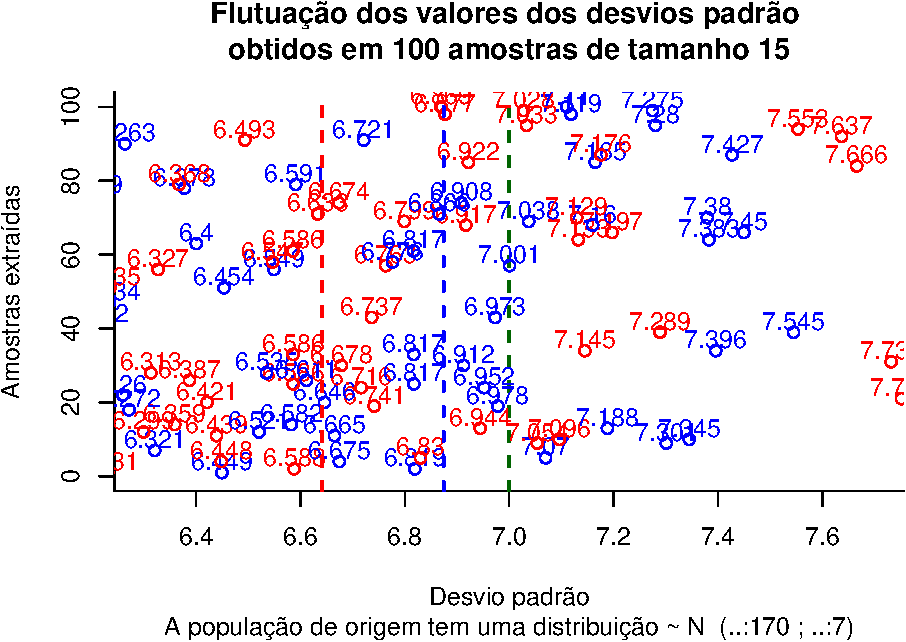
\includegraphics{apostila_files/figure-latex/unnamed-chunk-35-1} 

}

\caption{Mudanças na média pela multiplicação (divisão) de uma constante $k=1.2$}\label{fig:unnamed-chunk-35}
\end{figure}

\begin{itemize}
\tightlist
\item
  a soma dos desvios observados entre cada um dos valores assumidos pela variável \(X\) e sua média \(\stackrel{-}{x}\) é nula;
\item
  a soma dos quadrados dos desvios é mínima;
\item
  em uma distribuição de frequências, a soma dos produtos dos desvios entre a média o valor médio de cada uma das classes, pelas respectivas frequências é nula; e,
\item
  multiplicando-se (ou dividindo-se) todas as frequências de uma distribuição por uma constante arbitrária, a média aritmética não se altera.
\end{itemize}

Usando os dados das medidas das alturas dos 60 estudantes teremos o seguinte valor para a \textbf{média}:

\begin{Shaded}
\begin{Highlighting}[]
\FunctionTok{round}\NormalTok{(}\FunctionTok{mean}\NormalTok{(alturas),}\DecValTok{2}\NormalTok{)}
\end{Highlighting}
\end{Shaded}

\begin{verbatim}
## [1] 1.69
\end{verbatim}

\hypertarget{moda}{%
\subsubsection{Moda}\label{moda}}

Moda é o valor que ocorre com maior frequência na amostra. Uma amostra pode se apresentar como:
- unimodal;
- bimodal;
- plurimodal; ou,
- amodal.

\begin{Shaded}
\begin{Highlighting}[]
\NormalTok{tab\_alturas}\OtherTok{=}\FunctionTok{table}\NormalTok{(alturas)}

\NormalTok{tab\_alturas}
\end{Highlighting}
\end{Shaded}

\begin{verbatim}
## alturas
## 1.41 1.44 1.47 1.54 1.55 1.56 1.57 1.58 1.61 1.62 1.63 1.64 1.65 1.66 1.67 1.68 
##    1    1    1    1    1    3    1    2    1    2    1    2    4    5    4    3 
## 1.69 1.71 1.72 1.73 1.74 1.75 1.76 1.77 1.78 1.79 1.82 1.83 1.84 1.85 1.86 1.93 
##    1    2    2    5    1    1    2    1    2    1    1    2    1    1    1    1 
## 1.95    2 
##    1    1
\end{verbatim}

\begin{Shaded}
\begin{Highlighting}[]
\FunctionTok{barplot}\NormalTok{(tab\_alturas,}
        \AttributeTok{main=}\StringTok{"Valores observados da alturas dos estudantes"}\NormalTok{,}
        \AttributeTok{xlab=}\StringTok{"Altura (cm)"}\NormalTok{,}
        \AttributeTok{ylab=}\StringTok{"Quantidade observada (un)"}\NormalTok{,}
        \AttributeTok{ylim=}\FunctionTok{c}\NormalTok{(}\DecValTok{0}\NormalTok{,}\DecValTok{6}\NormalTok{),}
        \AttributeTok{col=}\StringTok{"blue"}\NormalTok{,}
        \AttributeTok{las=}\DecValTok{0}\NormalTok{, }
        \AttributeTok{hor=}\StringTok{"FALSE"}\NormalTok{)}
\end{Highlighting}
\end{Shaded}

\begin{figure}
\centering
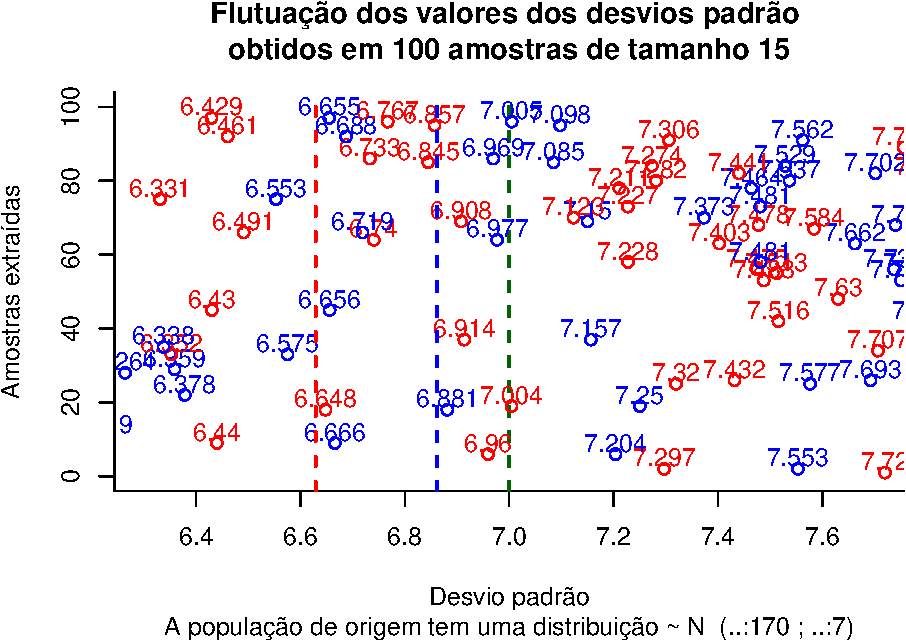
\includegraphics{apostila_files/figure-latex/unnamed-chunk-37-1.pdf}
\caption{\label{fig:unnamed-chunk-37}Bimodal: 1,66 m e 1,73 m}
\end{figure}

Usando os dados das medidas das alturas dos 60 estudantes teremos os seguintes valores para a \textbf{moda}:

\begin{Shaded}
\begin{Highlighting}[]
\CommentTok{\# função em R para extrair a moda:}

\NormalTok{Modes }\OtherTok{\textless{}{-}} \ControlFlowTok{function}\NormalTok{(x) \{}
\NormalTok{  ux }\OtherTok{\textless{}{-}} \FunctionTok{unique}\NormalTok{(x)}
\NormalTok{  tab }\OtherTok{\textless{}{-}} \FunctionTok{tabulate}\NormalTok{(}\FunctionTok{match}\NormalTok{(x, ux))}
\NormalTok{  ux[tab }\SpecialCharTok{==} \FunctionTok{max}\NormalTok{(tab)]}
\NormalTok{\}}

\FunctionTok{Modes}\NormalTok{(alturas)}
\end{Highlighting}
\end{Shaded}

\begin{verbatim}
## [1] 1.66 1.73
\end{verbatim}

\hypertarget{mediana}{%
\subsubsection{Mediana}\label{mediana}}

Mediana é o valor do \emph{i-ésimo} dado da amostra que ocupa a posição central na distribuição ordenada de modo crescente (ou decrescente), dividindo-a em duas partes de \emph{quantidades de dados iguais}.

Sendo uma medida separatriz de 50\%, equivale ao \(2^{o}\) quartil, ao \(5^{o}\) decil e ao \(50^{o}\) percentil.

1- amostra com um número \textbf{ímpar} (\(n\)) de elementos: a mediana será o valor do \_i-ésimo\} elemento (elemento na posição central) da amostra ordenada:

\[
Md=x_{i} 
\]

onde:

\begin{itemize}
\tightlist
\item
  \(i=\frac{n+1}{2}\) (\(n\) é o número de observações);
\end{itemize}

2- amostra com um número \textbf{par} (\(n\)) de elementos: a mediana será a \emph{média aritmética} dos elementos nas posições imediatamente anterior (\(i_{ant}\)) e posterior (\(i_{post}\)) à sua posição central virtual:

\[
Md=média(x_{i_{ant}} ; x_{i_{post}})
\]

onde:

\begin{itemize}
\tightlist
\item
  \(i_{ant} = \frac{n}{2}\) e \(i_{post} =\frac{n}{2}+1\) (\(n\) é o número de observações).
\end{itemize}

Mediana para dados apresentados na forma de uma distribuição de frequências:

\[
Md = l_{inf} + [ \frac{(\frac{n}{2} -  F_{(i_{md}-1)})}{n_{md}} ]\times \Delta_{i}
\]

onde:

\begin{itemize}
\tightlist
\item
  \(l_{inf}\): limite inferior da \textbf{classe mediana}: a classe que contem o elemento de ordem \(\frac{n}{2}\);
\item
  \(F_{(i_{md}-1)}\): é a frequência absoluta acumulada até a \textbf{classe anterior à classe mediana};
\item
  \(n_{md}\): é a frequência absoluta da \textbf{classe mediana}; e,
\item
  \(\Delta_{i}\): é o intervalo de cada classe.
\end{itemize}

Usando os dados das medidas das alturas dos 60 estudantes teremos o seguinte valor para a \textbf{mediana}:

\begin{Shaded}
\begin{Highlighting}[]
\FunctionTok{sort}\NormalTok{(alturas)}
\end{Highlighting}
\end{Shaded}

\begin{verbatim}
##  [1] 1.41 1.44 1.47 1.54 1.55 1.56 1.56 1.56 1.57 1.58 1.58 1.61 1.62 1.62 1.63
## [16] 1.64 1.64 1.65 1.65 1.65 1.65 1.66 1.66 1.66 1.66 1.66 1.67 1.67 1.67 1.67
## [31] 1.68 1.68 1.68 1.69 1.71 1.71 1.72 1.72 1.73 1.73 1.73 1.73 1.73 1.74 1.75
## [46] 1.76 1.76 1.77 1.78 1.78 1.79 1.82 1.83 1.83 1.84 1.85 1.86 1.93 1.95 2.00
\end{verbatim}

\begin{Shaded}
\begin{Highlighting}[]
\FunctionTok{median}\NormalTok{(alturas)}
\end{Highlighting}
\end{Shaded}

\begin{verbatim}
## [1] 1.675
\end{verbatim}

\hypertarget{diferentes-posiuxe7uxf5es-da-muxe9dia-moda-e-mediana}{%
\subsubsection{Diferentes posições da média, moda e mediana}\label{diferentes-posiuxe7uxf5es-da-muxe9dia-moda-e-mediana}}

Essas três medidas podem se apresentar com valores em posições alternadas quando as comparamos:

\begin{itemize}
\item
  quando a moda=mediana=média temos uma distribuição de frequências razoavelmente \textbf{simétrica};
\item
  quando a moda \(\leq\) mediana \(\leq\) média (há uma quantidade maior de dados com grandes valores, arrastando a média para a direita, para cima) temos uma distribuição de frequências \textbf{positivamente assimétrica}, ; e,\\
\item
  quando a moda \(\geq\) mediana \(\geq\) média (há uma quantidade maior de dados com pequenos valores, arrastando a média para a esquerda, para baixo) temos uma distribuição de frequências \textbf{negativamente assimétrica}.
\end{itemize}

\begin{Shaded}
\begin{Highlighting}[]
\FunctionTok{barplot}\NormalTok{(tab\_alturas,}
        \AttributeTok{main=}\StringTok{"Valores observados da alturas dos estudantes"}\NormalTok{,}
        \AttributeTok{xlab=}\StringTok{"Altura (cm)"}\NormalTok{,}
        \AttributeTok{ylab=}\StringTok{"Quantidade observada (un)"}\NormalTok{,}
        \AttributeTok{ylim=}\FunctionTok{c}\NormalTok{(}\DecValTok{0}\NormalTok{,}\DecValTok{6}\NormalTok{),}
        \AttributeTok{col=}\StringTok{"blue"}\NormalTok{,}
        \AttributeTok{las=}\DecValTok{0}\NormalTok{, }
        \AttributeTok{hor=}\StringTok{"FALSE"}\NormalTok{)}
\FunctionTok{abline}\NormalTok{(}\AttributeTok{v=}\FunctionTok{mean}\NormalTok{(}\FloatTok{19.9}\NormalTok{, }\FloatTok{21.1}\NormalTok{), }\AttributeTok{col=}\StringTok{"red"}\NormalTok{)}
\FunctionTok{text}\NormalTok{( }\FunctionTok{mean}\NormalTok{(}\FloatTok{19.9}\NormalTok{, }\FloatTok{21.1}\NormalTok{)}\SpecialCharTok{{-}}\FloatTok{0.5}\NormalTok{, }\DecValTok{5}\NormalTok{, }\StringTok{"Média=1,69 m"}\NormalTok{, }\AttributeTok{col =} \StringTok{"red"}\NormalTok{, }\AttributeTok{srt=}\DecValTok{90}\NormalTok{)}
\FunctionTok{abline}\NormalTok{(}\AttributeTok{v=}\FunctionTok{median}\NormalTok{(}\FloatTok{18.7}\NormalTok{ , }\FloatTok{19.9}\NormalTok{), }\AttributeTok{col=}\StringTok{"darkgreen"}\NormalTok{) }
\FunctionTok{text}\NormalTok{(}\FunctionTok{median}\NormalTok{(}\FloatTok{18.7}\NormalTok{ , }\FloatTok{19.9}\NormalTok{)}\SpecialCharTok{{-}}\FloatTok{0.5}\NormalTok{, }\DecValTok{5}\NormalTok{, }\StringTok{"Mediana=1,675 m"}\NormalTok{, }\AttributeTok{col =} \StringTok{"darkgreen"}\NormalTok{, }\AttributeTok{srt=}\DecValTok{90}\NormalTok{)}
\FunctionTok{abline}\NormalTok{(}\AttributeTok{v=}\FunctionTok{c}\NormalTok{(}\FloatTok{16.3}\NormalTok{, }\FloatTok{23.5}\NormalTok{), }\AttributeTok{col=}\StringTok{"darkgrey"}\NormalTok{) }
\FunctionTok{text}\NormalTok{(}\FunctionTok{c}\NormalTok{(}\FloatTok{16.3{-}0.5}\NormalTok{, }\FloatTok{23.5{-}0.5}\NormalTok{), }\DecValTok{5}\NormalTok{, }\FunctionTok{c}\NormalTok{(}\StringTok{"Moda=1,66"}\NormalTok{,}\StringTok{"Moda=1,73"}\NormalTok{), }\AttributeTok{col =} \StringTok{"darkgray"}\NormalTok{, }\AttributeTok{srt=}\DecValTok{90}\NormalTok{)}
\end{Highlighting}
\end{Shaded}

\begin{figure}

{\centering 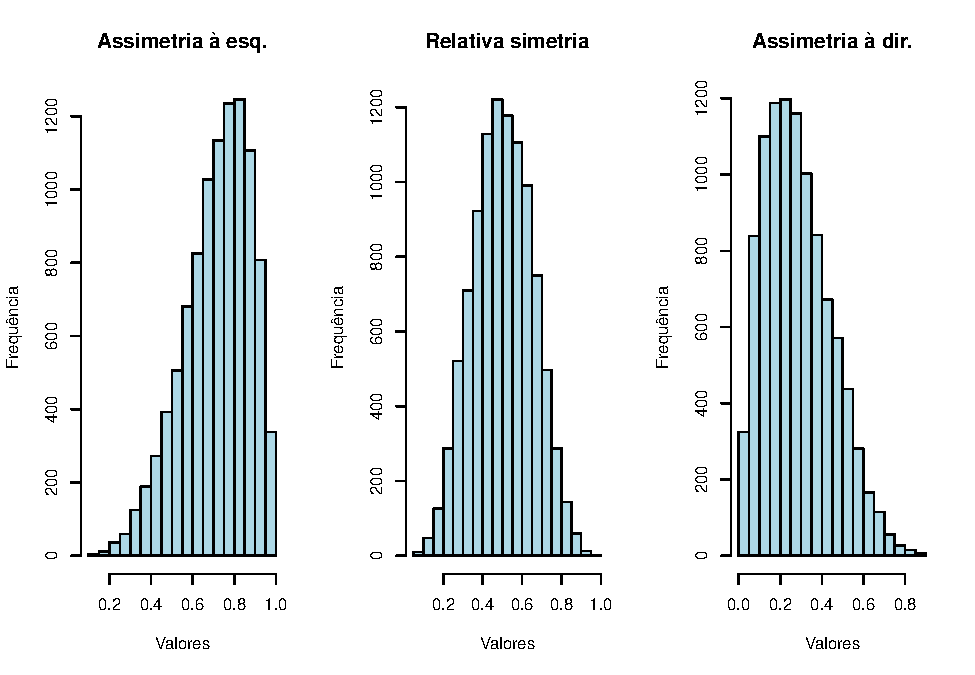
\includegraphics{apostila_files/figure-latex/unnamed-chunk-41-1} 

}

\caption{Valores observados das alturas dos estudantes e as posições da média, moda e mediana}\label{fig:unnamed-chunk-41}
\end{figure}

\begin{Shaded}
\begin{Highlighting}[]
\NormalTok{h1}\OtherTok{=}\FunctionTok{hist}\NormalTok{(alturas, }\AttributeTok{breaks=}\FunctionTok{seq}\NormalTok{(}\FloatTok{1.30}\NormalTok{ , }\FloatTok{2.10}\NormalTok{ , }\FloatTok{0.1}\NormalTok{), }\AttributeTok{main=} \StringTok{"Histograma das alturas dos estudantes"}\NormalTok{, }\AttributeTok{col=}\StringTok{"blue"}\NormalTok{, }
\AttributeTok{xlab=}\StringTok{"Classes de comprimento (cm)"}\NormalTok{, }\AttributeTok{ylab=}\StringTok{"Frequência absoluta observada (un)"}\NormalTok{ , }\AttributeTok{cex=}\FloatTok{0.7}\NormalTok{, }\AttributeTok{ylim=}\FunctionTok{c}\NormalTok{(}\DecValTok{0}\NormalTok{,}\DecValTok{30}\NormalTok{))}
\FunctionTok{text}\NormalTok{(h1}\SpecialCharTok{$}\NormalTok{mids,h1}\SpecialCharTok{$}\NormalTok{counts,}\AttributeTok{labels=}\NormalTok{h1}\SpecialCharTok{$}\NormalTok{counts, }\AttributeTok{adj=}\FunctionTok{c}\NormalTok{(}\FloatTok{0.5}\NormalTok{, }\SpecialCharTok{{-}}\FloatTok{0.5}\NormalTok{))}
\FunctionTok{abline}\NormalTok{(}\AttributeTok{v=}\FunctionTok{mean}\NormalTok{(alturas), }\AttributeTok{col=}\StringTok{"red"}\NormalTok{) }
\FunctionTok{text}\NormalTok{(}\FunctionTok{mean}\NormalTok{(alturas)}\SpecialCharTok{{-}}\FloatTok{0.01}\NormalTok{, }\DecValTok{28}\NormalTok{, }\StringTok{"Média=1,69 m"}\NormalTok{, }\AttributeTok{col =} \StringTok{"red"}\NormalTok{, }\AttributeTok{srt=}\DecValTok{90}\NormalTok{)}
\FunctionTok{abline}\NormalTok{(}\AttributeTok{v=}\FunctionTok{median}\NormalTok{(alturas), }\AttributeTok{col=}\StringTok{"darkgreen"}\NormalTok{) }
\FunctionTok{text}\NormalTok{(}\FunctionTok{median}\NormalTok{(alturas)}\SpecialCharTok{{-}}\FloatTok{0.01}\NormalTok{, }\FloatTok{27.2}\NormalTok{, }\StringTok{"Mediana=1,675 m"}\NormalTok{, }\AttributeTok{col =} \StringTok{"darkgreen"}\NormalTok{, }\AttributeTok{srt=}\DecValTok{90}\NormalTok{)}
\FunctionTok{abline}\NormalTok{(}\AttributeTok{v=}\FunctionTok{Modes}\NormalTok{(alturas), }\AttributeTok{col=}\StringTok{"darkgrey"}\NormalTok{) }
\FunctionTok{text}\NormalTok{(}\FunctionTok{Modes}\NormalTok{(alturas)}\SpecialCharTok{+}\FunctionTok{c}\NormalTok{(}\SpecialCharTok{{-}}\FloatTok{0.01}\NormalTok{, }\SpecialCharTok{{-}}\FloatTok{0.01}\NormalTok{), }\DecValTok{27}\NormalTok{, }\FunctionTok{c}\NormalTok{(}\StringTok{"Moda=1,66"}\NormalTok{,}\StringTok{"Moda=1,73"}\NormalTok{), }\AttributeTok{col =} \StringTok{"darkgray"}\NormalTok{, }\AttributeTok{srt=}\DecValTok{90}\NormalTok{)}
\end{Highlighting}
\end{Shaded}

\begin{figure}

{\centering 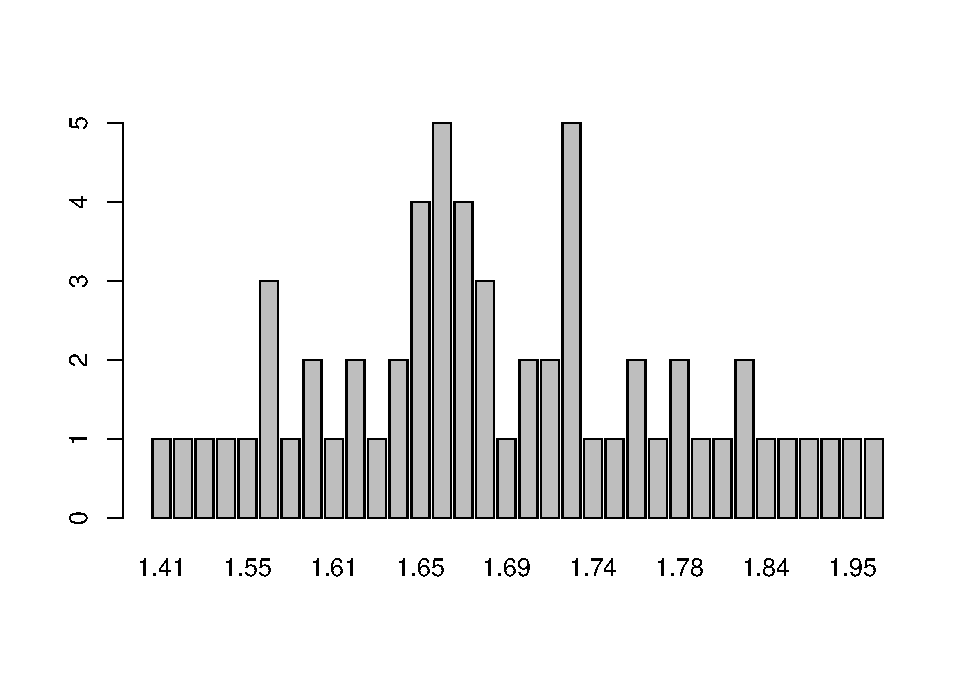
\includegraphics{apostila_files/figure-latex/unnamed-chunk-42-1} 

}

\caption{Histograma das alturas dos estudantes com as posições da média, moda e mediana}\label{fig:unnamed-chunk-42}
\end{figure}

\begin{figure}

{\centering 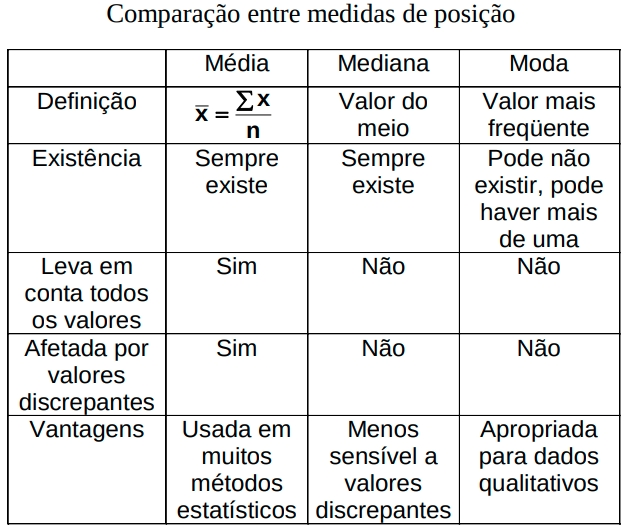
\includegraphics[width=0.5\linewidth]{images3/comp_sinteses} 

}

\caption{Quadro comparativo entre as medidas de tendência central (posição)}\label{fig:unnamed-chunk-43}
\end{figure}

\hypertarget{medidas-de-dispersuxe3o-variabilidade}{%
\subsection{Medidas de dispersão (variabilidade)}\label{medidas-de-dispersuxe3o-variabilidade}}

O conhecimento de uma medida de tendência central nos provê uma informação útil mas incompleta. As medidas de dispersão nos ajudam a ter uma perspectiva melhor dos dados.

\begin{itemize}
\tightlist
\item
  medidas absolutas: são expressas na mesma unidade de medida do fenômeno estudado.

  \begin{itemize}
  \tightlist
  \item
    amplitude total dos dados: diferença entre o maior e o menor dos valores observados; e,
  \item
    variância e desvio padrão: é considerada a mais útil das medidas de dispersão.
  \end{itemize}
\end{itemize}

\hfill\break

\begin{itemize}
\tightlist
\item
  medidas relativas: usadas para se comparar a variabilidade de duas ou mais distribuições, mesmo quando estas se refiram a diferentes fenômenos ou que sejam expressas em unidades diferentes.

  \begin{itemize}
  \tightlist
  \item
    coeficiente de variação; e,
  \item
    unidades padronizadas.
  \end{itemize}
\end{itemize}

\hypertarget{estimauxe7uxe3o-da-variuxe2ncia-e-desvio-padruxe3o.}{%
\subsubsection{Estimação da variância (e desvio padrão).}\label{estimauxe7uxe3o-da-variuxe2ncia-e-desvio-padruxe3o.}}

Sejam \(x_{1}, x_{2}, ..., x_{n}\) os \(n\) valores assumidos pela variável \(X\). Dá-se o nome de desvios a contar da média as diferenças entre cada uma das observações e a média: \(x_{i} - \stackrel{-}{x}\) com \(i=1,2,...,n\).

Não é possível considerar a possibilidade de se adotar o valor médio desses desvios pois uma das propriedades da média é que a soma dos desvios em torno de si é nula.

\[
\stackrel{-}{d} = \frac{\sum _{i=1}^{n}\left(x_{i}-\stackrel{-}{x}\right)}{n}
\]
\[
\sum _{i=1}^{n}\left(x_{i}-\stackrel{-}{x}\right)=0
\]

constitui-se numa restrição linear dos desvios porque qualquer \(n-1\) deles completamente determina o outro. Tampouco se considera a possibilidade de se adotar o valor médio desses desvios em módulo, pelas dificuldades teóricas em problemas de inferência.

\[
\stackrel{-}{d}  = \frac{\sum _{i=1}^{n}\left|x_{i}-\stackrel{-}{x}\right|}{n}
\]
Uma alternativa é adotar o valor médio do \textbf{quadrado} desses desvios.

\[
S^{2}=\frac{\sum _{i=1}^{n}\left(x_{i}-\stackrel{-}{x}\right)^{2}}{n-1}
\]

ou,

\[
S^{2}=\frac{1}{(n-1)} \times \left[ \sum _{i=1}^{n} (x_{i}^{2}) - \frac{({\sum _{i=1}^{n}x_{i})}^{2} }{n}\right]
\]

Diz-se que a variância amostral (variância \emph{ajustada}) possui \((n-1)\) graus de liberdade, denotado pela letra grega \(\nu\). A perda de \emph{um} grau de liberdade deve-se à necessidade de se substituir a média populacional desconhecida (\(\mu\)) por sua estimativa amostral (\(\stackrel{-}{x}\)), deduzida a partir dos dados coletados.

Pode-se demonstrar que em razão dessa restrição a melhor estimativa para a variância populacional é obtida dividindo-se a soma dos quadrados dos desvios por \((n-1)\). Assim \(S^{2}\) será um estimador não tendencioso para a variância amostral ao ser dividido por \((n-1)\)\}.

Uma medida de dispersão que apresenta a mesma unidade que a das observações originais é o \textbf{desvio-padrão}, definido como a raiz quadrada positiva da variância.

\[
S= \sqrt{\frac{\sum _{i=1}^{n}\left(x_{i}-\stackrel{-}{x}\right)^{2}}{n-1}}
\]

Tanto a variância quanto o desvio padrão indicam, em média, qual será o erro (desvio) cometido ao tentar substituir cada observação pela medida resumo do conjunto de dados (média).

Usando os dados das medidas das alturas dos 60 estudantes teremos o seguinte valor para a \textbf{variância} (com unidade igual a \(m^{2}\)) e o \textbf{desvio padrão} (com unidade igual a \(m\):

\begin{Shaded}
\begin{Highlighting}[]
\CommentTok{\# Variãncia}
\FunctionTok{var}\NormalTok{(alturas)}
\end{Highlighting}
\end{Shaded}

\begin{verbatim}
## [1] 0.0130809
\end{verbatim}

\begin{Shaded}
\begin{Highlighting}[]
\CommentTok{\# Desvio padrão}
\FunctionTok{sd}\NormalTok{(alturas) }
\end{Highlighting}
\end{Shaded}

\begin{verbatim}
## [1] 0.1143718
\end{verbatim}

Propriedades da variância:

\begin{itemize}
\tightlist
\item
  somando-se (ou subtraindo-se) cada um dos elementos do conjunto de dados por uma constante arbitrária, a variância (e o desvio padrão) não se altera; e,
\item
  multiplicando-se (ou dividindo-se) cada um dos elementos do conjunto de dados por uma constante arbitrária, a variância ficará multiplicada (ou dividida) pelo quadrado dessa constante. O desvio padrão fica multiplicado (ou dividido) por essa constante
\end{itemize}

\begin{Shaded}
\begin{Highlighting}[]
\CommentTok{\# Adicionando{-}se uma constante k=0.05}
\NormalTok{alturas\_ad}\OtherTok{=}\NormalTok{alturas}\FloatTok{+0.05}

\CommentTok{\# Variância não se altera}
\NormalTok{var\_ad}\OtherTok{=} \FunctionTok{var}\NormalTok{(alturas\_ad)}
\NormalTok{var\_ad}
\end{Highlighting}
\end{Shaded}

\begin{verbatim}
## [1] 0.0130809
\end{verbatim}

\begin{Shaded}
\begin{Highlighting}[]
\CommentTok{\# Multiplicando{-}se uma constante k=1.2}
\NormalTok{alturas\_mult}\OtherTok{=}\NormalTok{alturas}\SpecialCharTok{*}\FloatTok{1.2}

\CommentTok{\# Variância fica multiplicada (dividida) pelo quadrado dessa constante)}
\FunctionTok{var}\NormalTok{(alturas\_mult)}
\end{Highlighting}
\end{Shaded}

\begin{verbatim}
## [1] 0.0188365
\end{verbatim}

\begin{Shaded}
\begin{Highlighting}[]
\FunctionTok{all.equal}\NormalTok{(}\FunctionTok{var}\NormalTok{(alturas\_mult), }\FunctionTok{var}\NormalTok{(alturas)}\SpecialCharTok{*}\NormalTok{(}\FloatTok{1.2}\SpecialCharTok{\^{}}\DecValTok{2}\NormalTok{)) }
\end{Highlighting}
\end{Shaded}

\begin{verbatim}
## [1] TRUE
\end{verbatim}

\hypertarget{coeficiente-de-variauxe7uxe3o.}{%
\subsubsection{Coeficiente de variação.}\label{coeficiente-de-variauxe7uxe3o.}}

O coeficiente de variação (uma medidad adimensional) é dado pela razão do desvio padrão pela média:

\[
CV= 100\cdot(\frac{s}{\stackrel{-}{x}})
\]

\hypertarget{padronizauxe7uxe3o-z-scores}{%
\subsubsection{\texorpdfstring{Padronização (\emph{z-scores})}{Padronização (z-scores)}}\label{padronizauxe7uxe3o-z-scores}}

À conversão do valor assumido por uma variável em unidades de desvio padrão acima (ou abaixo) do valor médio de sua distribuição é dado o nome de \emph{padronização}. Essa métrica permite comparações com outras, procedentes de outros fenômenos.

Para padronizar (achar o seu \emph{z-score} Z) o valor de uma variável procede-se segundo a fórmula:

\[
Z=\frac{x_{i} - \stackrel{-}{x}}{s}
\]

O valor \(Z\) expressa quantos desvios esse dado está acima (ou abaixo) da média da distribuição.

Pelo \emph{Teorema de Tchebichev} pode-se estimar a probabilidade mínima dos dados situados a certa distância de \(k\) desvios da média dessa distribuição:

\[
P(|X-\mu|\ge k\sigma) \leq 1 - \frac{1}{k^{2}}
\]
Assim, se \(k=2\) \textbf{ao menos} 75\% das observações devem estar entre a média e dois desvios padrões acima ou abaixo da média.

\begin{Shaded}
\begin{Highlighting}[]
\NormalTok{med}\OtherTok{=}\FunctionTok{round}\NormalTok{(}\FunctionTok{mean}\NormalTok{(alturas),}\DecValTok{2}\NormalTok{)}
\NormalTok{desv}\OtherTok{=} \FunctionTok{round}\NormalTok{(}\FunctionTok{sd}\NormalTok{(alturas),}\DecValTok{2}\NormalTok{)}
\end{Highlighting}
\end{Shaded}

No exemplo das alturas dos estudantes temos a média de 1.69 m e um desvio padrão de 0.11 m. Assim, \textbf{ao menos} 75\% das alturas deverão estar entre 1.47 m e 1.91 m.

\begin{Shaded}
\begin{Highlighting}[]
\FunctionTok{sort}\NormalTok{(alturas)}
\end{Highlighting}
\end{Shaded}

\begin{verbatim}
##  [1] 1.41 1.44 1.47 1.54 1.55 1.56 1.56 1.56 1.57 1.58 1.58 1.61 1.62 1.62 1.63
## [16] 1.64 1.64 1.65 1.65 1.65 1.65 1.66 1.66 1.66 1.66 1.66 1.67 1.67 1.67 1.67
## [31] 1.68 1.68 1.68 1.69 1.71 1.71 1.72 1.72 1.73 1.73 1.73 1.73 1.73 1.74 1.75
## [46] 1.76 1.76 1.77 1.78 1.78 1.79 1.82 1.83 1.83 1.84 1.85 1.86 1.93 1.95 2.00
\end{verbatim}

\begin{Shaded}
\begin{Highlighting}[]
\CommentTok{\# Duas observações menores que 1,47m e trẽs maiores que 1,91m.}
\CommentTok{\# Assim, 54 observações dentro do intervalo, equivalendo a 91,66\% do total.}
\end{Highlighting}
\end{Shaded}

\hypertarget{medidas-de-subdivisuxe3o-separatrizes}{%
\subsection{Medidas de subdivisão (separatrizes)}\label{medidas-de-subdivisuxe3o-separatrizes}}

Separatrizes (quantis) são valores que delimitam uma proporção de observações existentes de um conjunto de dados previamente ordenados menores que ele.

De modo geral, um \emph{quantil} de ordem \(p\) (ou também \(p-quantil\), indicado por \(q_{p}\)) é uma medida onde \(p\) é uma proporção qualquer (limitada no intervalo 0 \textless{} p \textless{} 1), tal que 100\(p\)\% das observações sejam menores que seu valor \(q_{p}\). Os \emph{quantis} mais relevantes são:

\begin{itemize}
\tightlist
\item
  1\(^{o}\) Quartil (\(q_{0,25}\)): 25\% dos dados possuem valores abaixo desse valor e 75\% estão acima;
\item
  2\(^{o}\) Quartil ou mediana (\(q_{0,50}\)): 50\% dos dados possuem valores abaixo desse valor e 50\% estão acima; e,
\item
  3\(^{o}\) Quartil (\(q_{0,75}\)): 75\% dos dados possuem valores abaixo desse valor e 25\% estão acima.
\end{itemize}

Para se calcular a \textbf{posição} \emph{L} de um quantil de ordem \emph{p} em um rol de dados, pode-se usar a seguinte regra:

\[
L=\frac{p}{100} \times (n+1)
\]

Duas situações possíveis para a posição \textbf{L}: ser um número fracionário ou inteiro:

\begin{itemize}
\tightlist
\item
  se a posição \textbf{L for fracionária} deve-se fazer a média entre os dois valores que estão nas posições imediatamente anterior e imediatamente posterior à posição calculada;
\item
  se a posição \textbf{L for um inteiro} essa será a posição do valor referente ao quantil desejado.
\end{itemize}

Onde:

\begin{itemize}
\tightlist
\item
  \emph{p} é a \textbf{ordem} do quantil em \% (50\% no caso mediana, por exemplo);
\item
  \emph{n} é o número de dados do rol; e,
\item
  \emph{L} é a \textbf{posição} do valor referente ao quantil desejado.
\end{itemize}

Juntamente com as observações mínima (\(x_{i}\)) e máxima (\(x_{n}\)), o 1\(^{o}\), 2\(^{o}\) e 3\(^{o}\) Quartis são importantes para se ter uma boa idéia da assimetria da distribuição dos dados.

Para uma distribuição simétrica (ou aproximadamente simétrica) deveremos observar (Distribuição Gaussiana):

\begin{itemize}
\tightlist
\item
  a dispersão inferior: \(q_{2} - x_{1} \approx x_{n} - q_{2}\) à dispersão superior ;
\item
  \(q_{2} - q_{1} \approx q_{3} - q_{2}\); e,
\item
  \(q_{1} - x_{1} \approx x_{n} - q_{3}\).
\end{itemize}

\begin{Shaded}
\begin{Highlighting}[]
\FunctionTok{set.seed}\NormalTok{(}\DecValTok{1000}\NormalTok{)}
\NormalTok{y\_normal}\OtherTok{=}\FunctionTok{rnorm}\NormalTok{(}\DecValTok{1000}\NormalTok{ , }\DecValTok{20}\NormalTok{ , }\DecValTok{5}\NormalTok{ )}
\FunctionTok{range}\NormalTok{(y\_normal)}
\end{Highlighting}
\end{Shaded}

\begin{verbatim}
## [1]  3.191432 33.350358
\end{verbatim}

\begin{Shaded}
\begin{Highlighting}[]
\FunctionTok{quantile}\NormalTok{(y\_normal)}
\end{Highlighting}
\end{Shaded}

\begin{verbatim}
##        0%       25%       50%       75%      100% 
##  3.191432 16.685004 20.112604 23.220489 33.350358
\end{verbatim}

\begin{Shaded}
\begin{Highlighting}[]
\FunctionTok{hist}\NormalTok{(y\_normal, }\AttributeTok{prob=}\ConstantTok{TRUE}\NormalTok{, }\AttributeTok{breaks=}\DecValTok{20}\NormalTok{, }\AttributeTok{ylab=}\StringTok{""}\NormalTok{, }\AttributeTok{xlab=}\StringTok{""}\NormalTok{, }\AttributeTok{yaxt=}\StringTok{"n"}\NormalTok{,  }\AttributeTok{xaxt=}\StringTok{"n"}\NormalTok{, }\AttributeTok{main=}\StringTok{"Histograma de uma variável com Distribuição Normal"}\NormalTok{)}
\FunctionTok{curve}\NormalTok{(}\FunctionTok{dnorm}\NormalTok{(x, }\FunctionTok{mean}\NormalTok{(y\_normal), }\FunctionTok{sd}\NormalTok{(y\_normal)), }\AttributeTok{add=}\ConstantTok{TRUE}\NormalTok{, }\AttributeTok{col=}\StringTok{"darkblue"}\NormalTok{, }\AttributeTok{lwd=}\DecValTok{2}\NormalTok{)}

\FunctionTok{abline}\NormalTok{(}\AttributeTok{v=}\FloatTok{3.19}\NormalTok{, }\AttributeTok{col=}\StringTok{"red"}\NormalTok{) }
\FunctionTok{text}\NormalTok{(}\FloatTok{3.19} \SpecialCharTok{{-}}\FloatTok{0.6}\NormalTok{, }\FloatTok{0.02}\NormalTok{, }\StringTok{"x(1)"}\NormalTok{, }\AttributeTok{col =} \StringTok{"red"}\NormalTok{, }\AttributeTok{srt=}\DecValTok{90}\NormalTok{)}
\FunctionTok{abline}\NormalTok{(}\AttributeTok{v=}\FloatTok{16.68}\NormalTok{, }\AttributeTok{col=}\StringTok{"red"}\NormalTok{) }
\FunctionTok{text}\NormalTok{(}\FloatTok{16.68} \SpecialCharTok{{-}}\FloatTok{0.6}\NormalTok{, }\FloatTok{0.02}\NormalTok{, }\StringTok{"1? Quartil"}\NormalTok{, }\AttributeTok{col =} \StringTok{"red"}\NormalTok{, }\AttributeTok{srt=}\DecValTok{90}\NormalTok{)}
\FunctionTok{abline}\NormalTok{(}\AttributeTok{v=}\FloatTok{20.11}\NormalTok{, }\AttributeTok{col=}\StringTok{"red"}\NormalTok{) }
\FunctionTok{text}\NormalTok{(}\FloatTok{20.11} \SpecialCharTok{{-}} \FloatTok{0.6}\NormalTok{, }\FloatTok{0.02}\NormalTok{, }\StringTok{"2? Quartil"}\NormalTok{, }\AttributeTok{col =} \StringTok{"red"}\NormalTok{, }\AttributeTok{srt=}\DecValTok{90}\NormalTok{)}
\FunctionTok{abline}\NormalTok{(}\AttributeTok{v=}\FloatTok{23.22}\NormalTok{, }\AttributeTok{col=}\StringTok{"red"}\NormalTok{) }
\FunctionTok{text}\NormalTok{(}\FloatTok{23.22} \SpecialCharTok{{-}} \FloatTok{0.6}\NormalTok{, }\FloatTok{0.02}\NormalTok{, }\StringTok{"3? Quartil"}\NormalTok{, }\AttributeTok{col =} \StringTok{"red"}\NormalTok{, }\AttributeTok{srt=}\DecValTok{90}\NormalTok{)}
\FunctionTok{abline}\NormalTok{(}\AttributeTok{v=}\FloatTok{33.35}\NormalTok{, }\AttributeTok{col=}\StringTok{"red"}\NormalTok{) }
\FunctionTok{text}\NormalTok{(}\FloatTok{33.35} \SpecialCharTok{{-}}\FloatTok{0.6}\NormalTok{, }\FloatTok{0.02}\NormalTok{, }\StringTok{"x(n)"}\NormalTok{, }\AttributeTok{col =} \StringTok{"red"}\NormalTok{, }\AttributeTok{srt=}\DecValTok{90}\NormalTok{)}
\end{Highlighting}
\end{Shaded}

\begin{figure}

{\centering 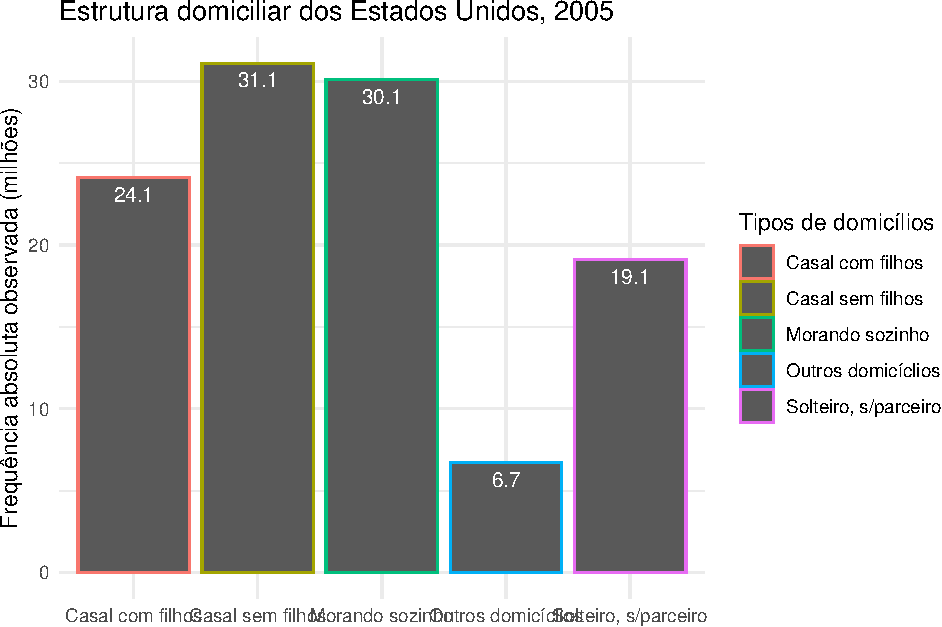
\includegraphics{apostila_files/figure-latex/unnamed-chunk-48-1} 

}

\caption{Histograma de uma variável com Distribuição Normal (média 20 e variãncia 5}\label{fig:unnamed-chunk-48}
\end{figure}

\hypertarget{medidas-de-forma-assimetria-curtose}{%
\section{Medidas de forma (assimetria \& curtose)}\label{medidas-de-forma-assimetria-curtose}}

Quando analisamos o histograma (a representação gráfica da distribuição das frequências dos valores agrupados em classes) de uma determinada variável, não é muito comum que ele se mostre simétrico tal como seria se os dados fossem distribuídos de modo exatamente Normal.

Ao observarmos que a cauda se mostra mais alongada para a direita (indicativo da existência de uma quantidade maior de dados com grandes valores, \emph{arrastando} a média para a direita: moda \(<\) mediana \(<\) média) diz-se que a \emph{distribuição é assimétrica à direita}. Na situação oposta (moda \(>\) mediana \(>\) média) diz-se que ela é \emph{assimétrica à esquerda}.

\begin{Shaded}
\begin{Highlighting}[]
\NormalTok{a}\OtherTok{=}\FunctionTok{rbeta}\NormalTok{(}\DecValTok{10000}\NormalTok{,}\DecValTok{5}\NormalTok{,}\DecValTok{2}\NormalTok{)}
\NormalTok{c}\OtherTok{=}\FunctionTok{rbeta}\NormalTok{(}\DecValTok{10000}\NormalTok{,}\DecValTok{5}\NormalTok{,}\DecValTok{5}\NormalTok{)}
\NormalTok{b}\OtherTok{=}\FunctionTok{rbeta}\NormalTok{(}\DecValTok{10000}\NormalTok{,}\DecValTok{2}\NormalTok{,}\DecValTok{5}\NormalTok{)}

\FunctionTok{par}\NormalTok{(}\AttributeTok{mfrow=}\FunctionTok{c}\NormalTok{(}\DecValTok{1}\NormalTok{,}\DecValTok{3}\NormalTok{))}
\FunctionTok{hist}\NormalTok{(a, }
     \AttributeTok{xlab=}\StringTok{"Valores"}\NormalTok{,}\AttributeTok{col =} \StringTok{\textquotesingle{}lightblue\textquotesingle{}}\NormalTok{,}
     \AttributeTok{ylab=}\StringTok{"Frequência"}\NormalTok{,}
     \AttributeTok{main=}\StringTok{"Assimetria à esq."}\NormalTok{)}
\FunctionTok{hist}\NormalTok{(c, }
     \AttributeTok{xlab=}\StringTok{"Valores"}\NormalTok{,}\AttributeTok{col =} \StringTok{\textquotesingle{}lightblue\textquotesingle{}}\NormalTok{,}
     \AttributeTok{ylab=}\StringTok{"Frequência"}\NormalTok{,}
     \AttributeTok{main=}\StringTok{"Relativa simetria"}\NormalTok{)}
\FunctionTok{hist}\NormalTok{(b, }
     \AttributeTok{xlab=}\StringTok{"Valores"}\NormalTok{,}\AttributeTok{col =} \StringTok{\textquotesingle{}lightblue\textquotesingle{}}\NormalTok{,}
     \AttributeTok{ylab=}\StringTok{"Frequência"}\NormalTok{,}
     \AttributeTok{main=}\StringTok{"Assimetria à dir."}\NormalTok{)}
\end{Highlighting}
\end{Shaded}

\begin{figure}

{\centering 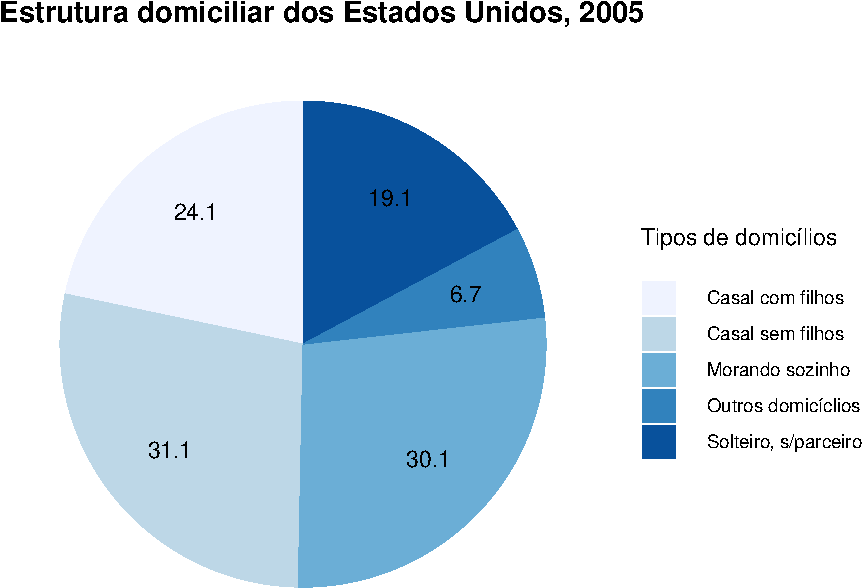
\includegraphics[width=0.8\linewidth]{apostila_files/figure-latex/unnamed-chunk-49-1} 

}

\caption{Diferentes formas na distribuição dos dados}\label{fig:unnamed-chunk-49}
\end{figure}

De modo assemelhado, o histograma pode denotar uma forma mais \emph{plana} ou menos \emph{aguda}, onde um \emph{cume} mostra-se mais destacado.

Nesse aspecto da forma, uma variável com distribuição Gaussiana apresentaria uma curva a que denominamos \emph{mesocúrtica}. Distribuições com um aspecto mais plano são denominadas de \emph{platicúrticas} e as com um cume agudo são denominadas \emph{leptocúrticas}.

A curtose é uma medida da agudeza da distribuição dos dados em relação à distribuição Gaussiana.

\begin{figure}

{\centering 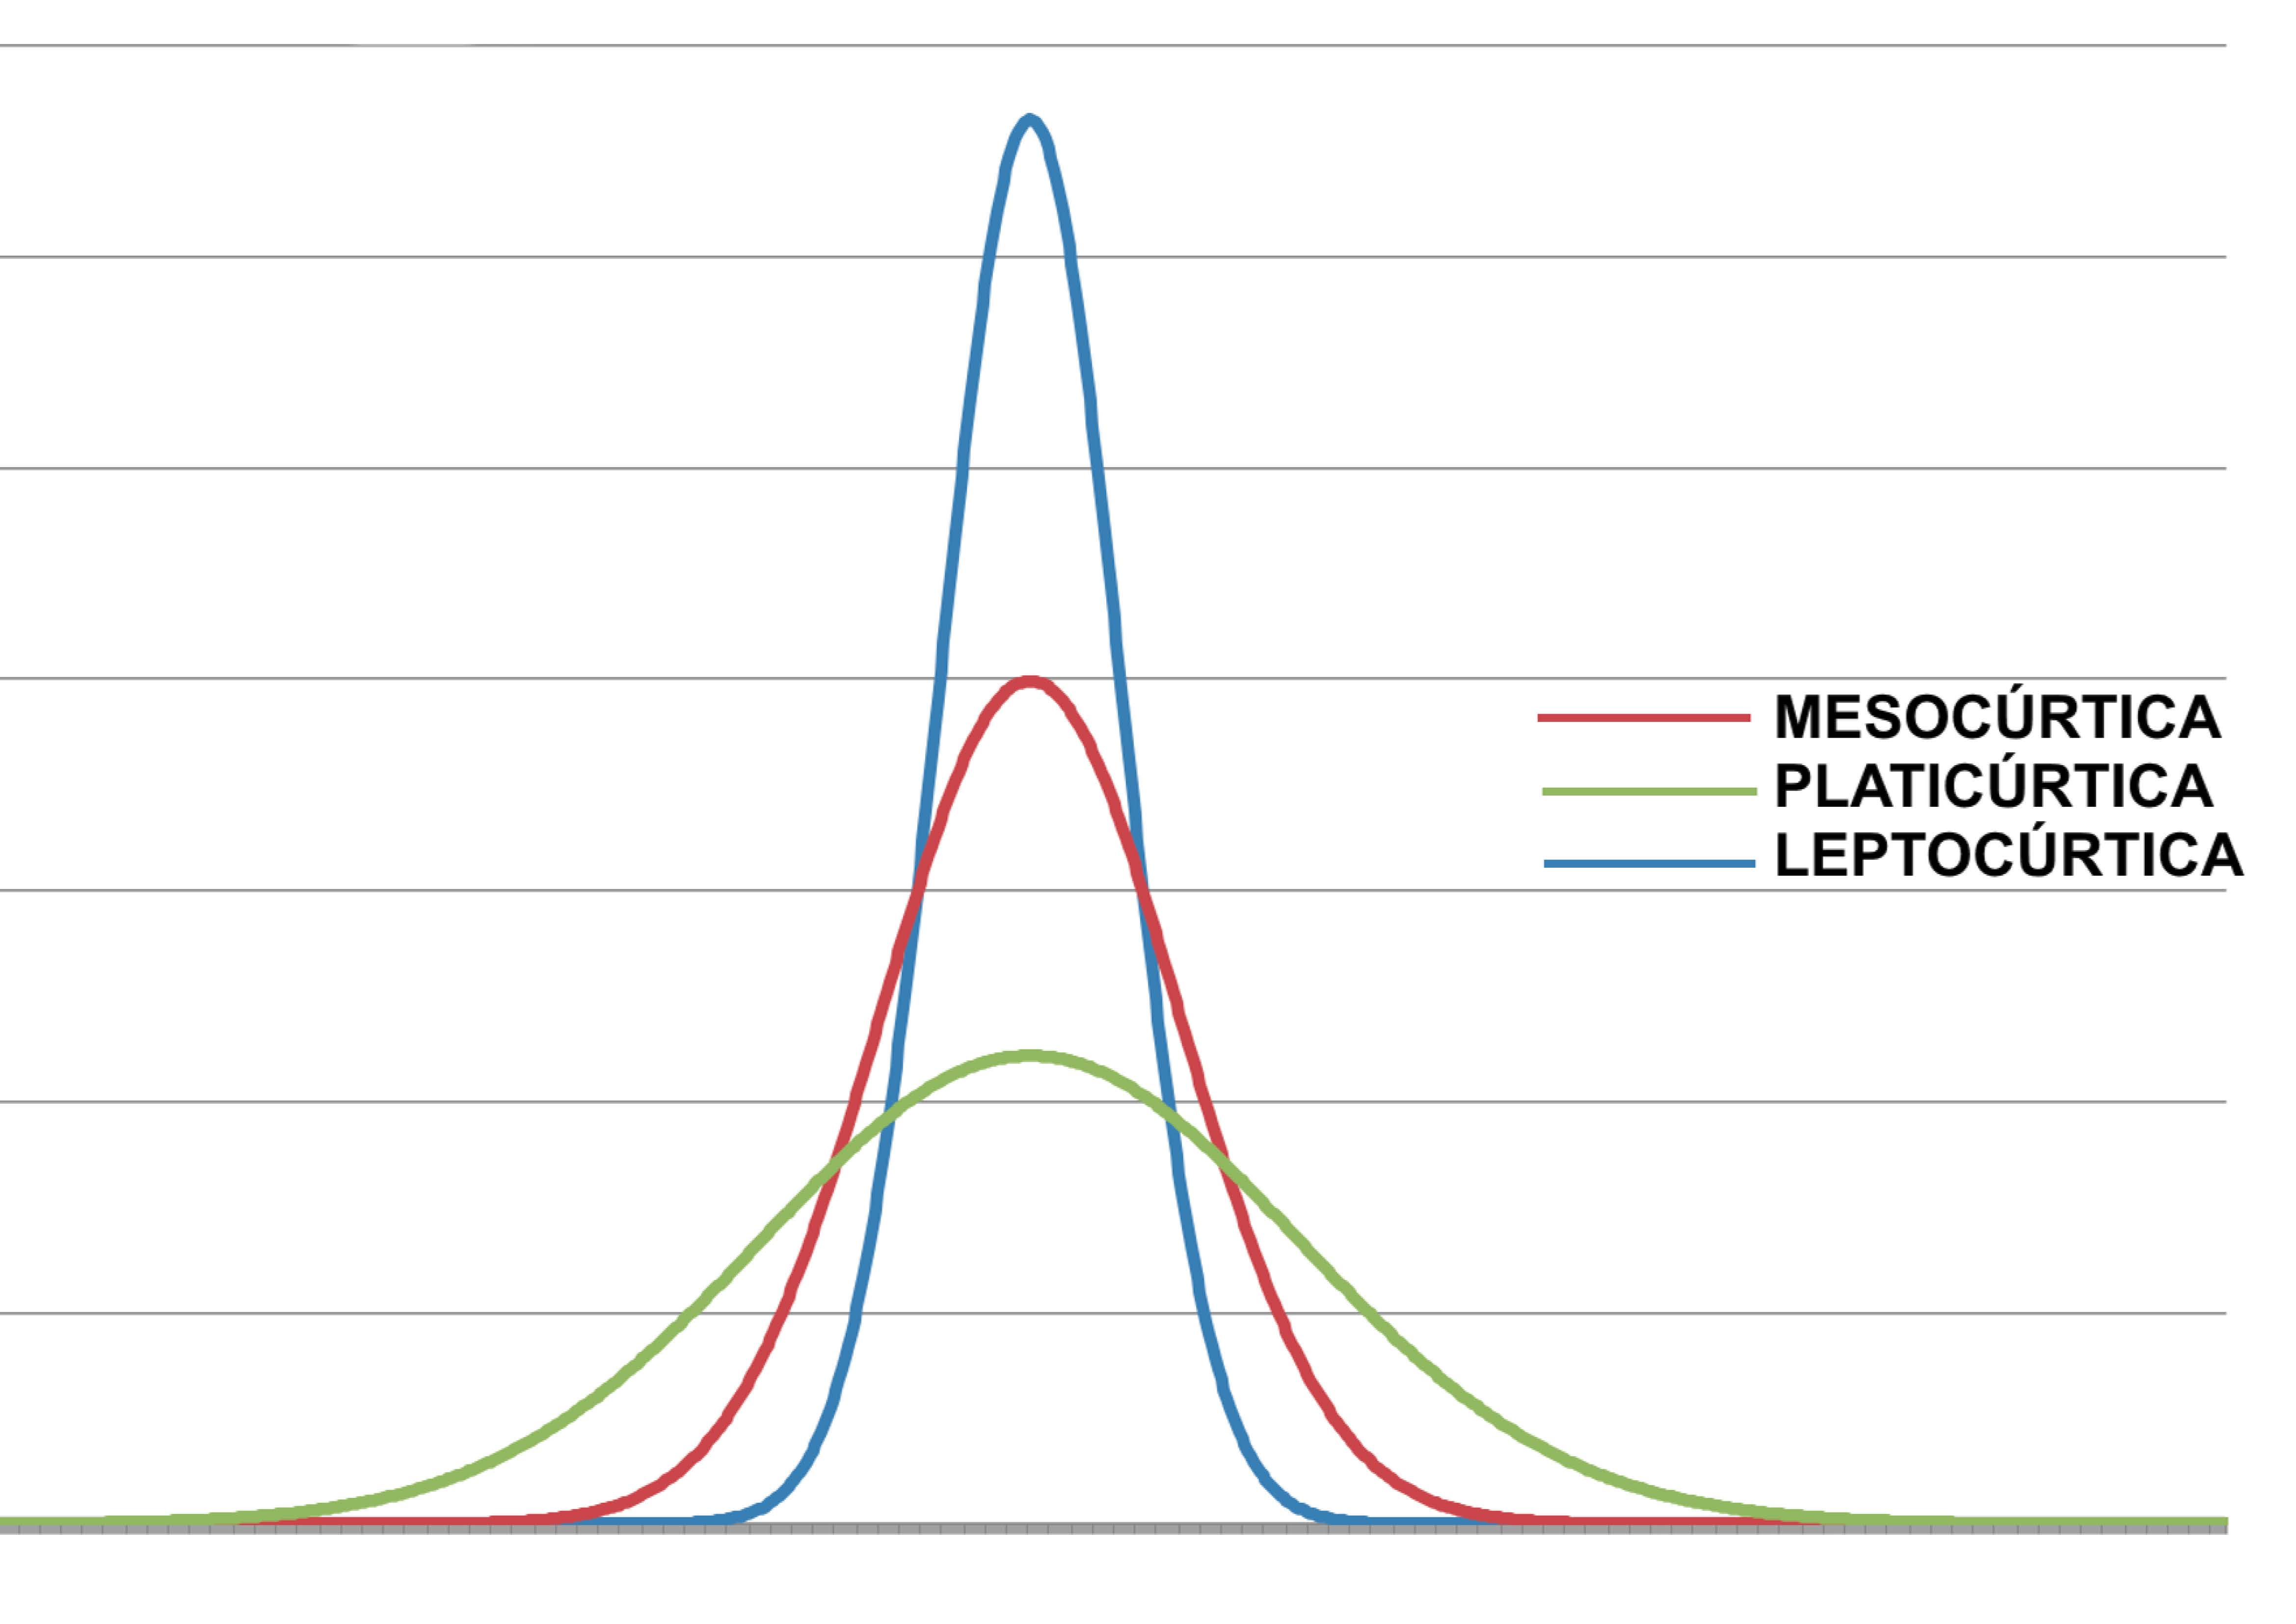
\includegraphics[width=0.5\linewidth]{images3/curtose} 

}

\caption{Diferentes aspectos de uma distribuição quanto à sua inclinação}\label{fig:unnamed-chunk-50}
\end{figure}

Essas possíveis variações na forma de uma distribuição podem ser numericamente quantificadas através dos \emph{coeficientes de assimetria e curtose}.

Uma das medidas do coeficiente de assimetria é através do \emph{primeiro ou segundo coeficientes de Pearson}, dados pelas seguintes relações:

\begin{itemize}
\tightlist
\item
  Primeiro coeficiente de assimetria de Pearson: \(AS= \frac{ \stackrel{-}{x} - M_{o} }{ s }\)
\item
  Segundo coeficiente de assimetria de Pearson: \(AS = \frac{ 3 ( \stackrel{-}{x} - M_{d}) } { s }\)
\end{itemize}

Onde:

\begin{itemize}
\tightlist
\item
  \(\stackrel{-}{x}\) é a média;
\item
  \(M_{o}\) é a moda;
\item
  \(S\) é o desvio padrão; e,
\item
  \(M_{d}\) é a mediana.
\end{itemize}

A \emph{assimetria} é classificada do modo seguinte:

\begin{itemize}
\tightlist
\item
  AS=0: distribuição simétrica;
\item
  AS\textless0: distribuição com assimetria negativa; e,
\item
  AS\textgreater0: distribuição com assimetria positiva.
\end{itemize}

Uma das medidas do coeficiente de curtose é através da seguinte relação entre \emph{quartis} e \emph{percentis}:

\[
K = \frac{\frac{Q_{3} - Q_{1}}{2}   }   {P_{90} - P_{10}} 
\]

Onde:

\begin{itemize}
\tightlist
\item
  \(Q_{3}\) = \(3^{o}\) quartil;
\item
  \(Q_{1}\) = \(1^{o}\) quartil;
\item
  \(P_{90}\) = \(90^{o}\) percentil; e,
\item
  \(P_{10}\) = \(10^{o}\) percentil.
\end{itemize}

O \emph{coeficiente de curtose} é classificado do modo seguinte:

\begin{itemize}
\tightlist
\item
  k = 0; 263: distribuição mesocúrtica;
\item
  k \textless{} 0; 263: distribuição leptocúrtica; e,
\item
  k \textgreater{} 0; 263: distribuição platicúrtica.
\end{itemize}

\hypertarget{apresentauxe7uxe3o-gruxe1fica-de-dados}{%
\section{Apresentação gráfica de dados}\label{apresentauxe7uxe3o-gruxe1fica-de-dados}}

Uma apresentação na forma gráfica torna ainda mais fácil a visualização das informações contidas nos dados.

Há uma gama enorme de gráficos para a representação de dados a depender de sua natureza (qualitativa ou quantitativa). Alguns dos tipos mais comuns são:

\begin{enumerate}
\def\labelenumi{\arabic{enumi}.}
\tightlist
\item
  qualitativas
\end{enumerate}

\begin{itemize}
\tightlist
\item
  ranking: barras;
\item
  parte em relação ao todo: setores;
\end{itemize}

\begin{enumerate}
\def\labelenumi{\arabic{enumi}.}
\setcounter{enumi}{1}
\tightlist
\item
  quantitativas
\end{enumerate}

\begin{itemize}
\tightlist
\item
  ranking: barras;
\item
  parte em relação ao todo: setores;
\item
  dispersão unidimensional;
\item
  distribuição: histograma e o \emph{box plot};
\item
  correlação: pontos dispersos; e,
\item
  tendência: linha
\end{itemize}

Se modificarmos o diagrama de ramos e folhas dos comprimentos e quantidades observadas, representando cada uma das alturas medidas por um \emph{retângulo} cujas alturas sejam proporcionais à quantidade contada de cada uma dessas alturas teremos um \emph{Gráfico de barras}.

\hypertarget{barras}{%
\subsection{Barras}\label{barras}}

\begin{Shaded}
\begin{Highlighting}[]
\NormalTok{tab\_alturas}\OtherTok{=}\FunctionTok{table}\NormalTok{(alturas)}

\FunctionTok{barplot}\NormalTok{(tab\_alturas,}
        \AttributeTok{main=}\StringTok{"Valores observados da alturas dos estudantes"}\NormalTok{,}
        \AttributeTok{xlab=}\StringTok{"Altura (cm)"}\NormalTok{,}
        \AttributeTok{ylab=}\StringTok{"Quantidade observada (un)"}\NormalTok{,}
        \AttributeTok{ylim=}\FunctionTok{c}\NormalTok{(}\DecValTok{0}\NormalTok{,}\DecValTok{6}\NormalTok{),}
        \AttributeTok{col=}\StringTok{"blue"}\NormalTok{,}
        \AttributeTok{las=}\DecValTok{0}\NormalTok{, }
        \AttributeTok{hor=}\StringTok{"FALSE"}\NormalTok{)}
\end{Highlighting}
\end{Shaded}

\begin{figure}
\centering
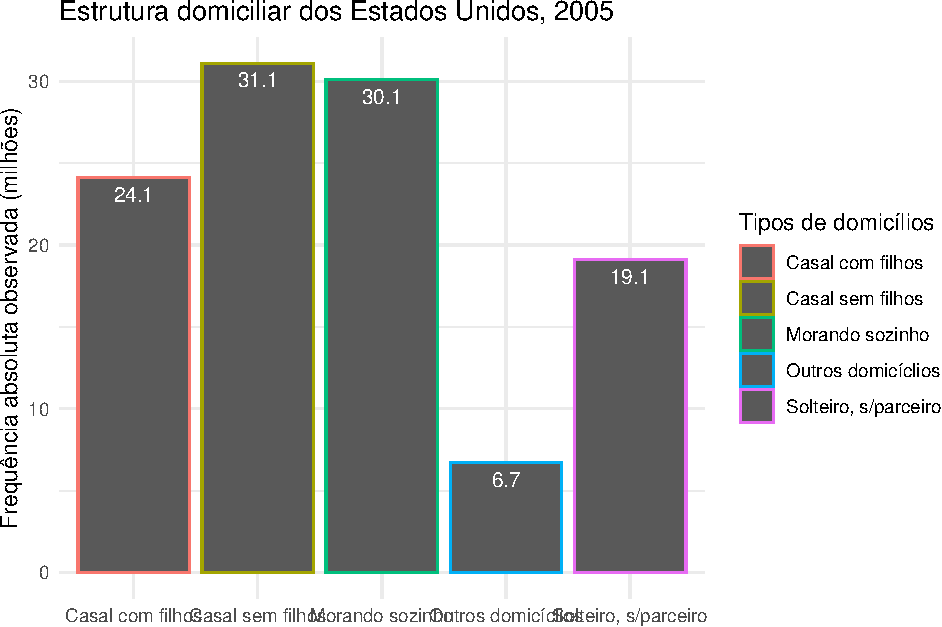
\includegraphics{apostila_files/figure-latex/unnamed-chunk-51-1.pdf}
\caption{\label{fig:unnamed-chunk-51}Gráfico de barras dos dados brutos: uma barra para cada observação e sua altura expressando o número de observações com esse valor}
\end{figure}

Para dados quantitativos, o agrupamento dos valores brutos observados em classes (cada uma com um valor mínimo e máximo fixado) permite a geração de um \emph{Histograma}, um tipo diferente de \emph{Gráfico de barras} onde cada coluna está unida às colunas imediatamente adjacentes (indicando a continuidade de valores das medidas) e sua altura expressa a quantidade de observações contidas nessa classe.

Se adotarmos arbitrariamente como classes para as alturas: 1,30-1,40; 1,40-1,50; 1,50-1,60; 1,60-1,70; 1,70-1,80; 1,80-1,90; 1,90-2,00; 2,00-2,10, o histograma terá esse aspecto:

\begin{Shaded}
\begin{Highlighting}[]
\FunctionTok{hist}\NormalTok{(alturas, }\AttributeTok{breaks=}\FunctionTok{seq}\NormalTok{(}\FloatTok{1.30}\NormalTok{ , }\FloatTok{2.10}\NormalTok{ , }\FloatTok{0.10}\NormalTok{), }\AttributeTok{main=} \StringTok{"Histograma das alturas dos estudantes"}\NormalTok{, }\AttributeTok{col=}\StringTok{"blue"}\NormalTok{, }
\AttributeTok{xlab=}\StringTok{"Classes de altura (m)"}\NormalTok{, }\AttributeTok{ylab=}\StringTok{"Frequência observada (un)"}\NormalTok{ , }\AttributeTok{cex=}\FloatTok{0.7}\NormalTok{, }\AttributeTok{ylim=}\FunctionTok{c}\NormalTok{(}\DecValTok{0}\NormalTok{,}\DecValTok{30}\NormalTok{))}
\FunctionTok{text}\NormalTok{(h1}\SpecialCharTok{$}\NormalTok{mids,h1}\SpecialCharTok{$}\NormalTok{counts,}\AttributeTok{labels=}\NormalTok{h1}\SpecialCharTok{$}\NormalTok{counts, }\AttributeTok{adj=}\FunctionTok{c}\NormalTok{(}\FloatTok{0.5}\NormalTok{, }\SpecialCharTok{{-}}\FloatTok{0.5}\NormalTok{))}
\end{Highlighting}
\end{Shaded}

\begin{figure}
\centering
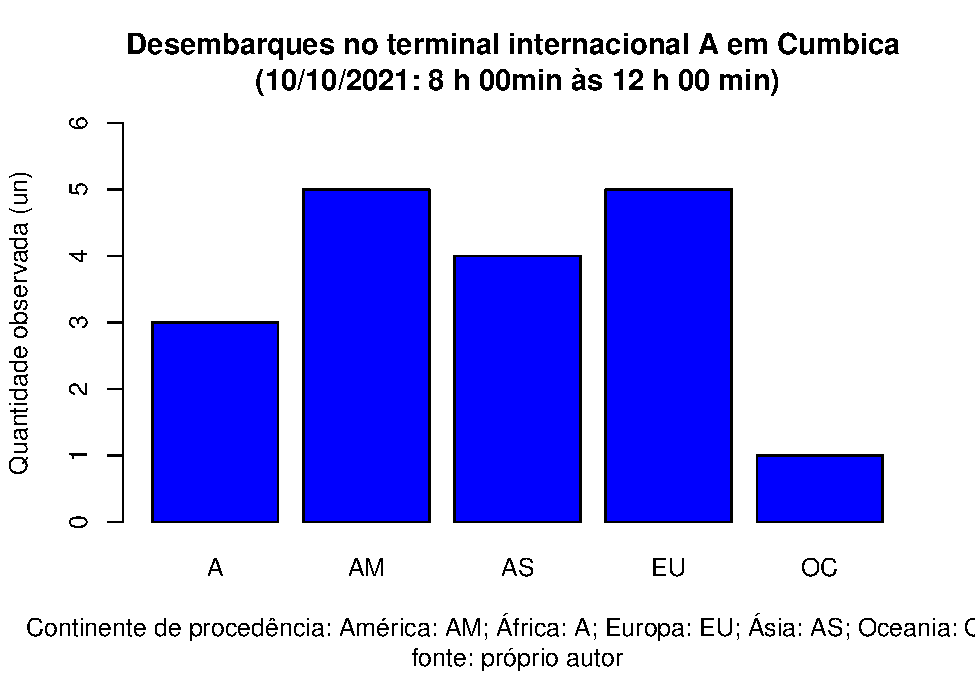
\includegraphics{apostila_files/figure-latex/unnamed-chunk-52-1.pdf}
\caption{\label{fig:unnamed-chunk-52}Histograma das alturas dos estudantes. Uma barra para cada classe de altura e sua altura expressando a quantidade de observações com valores dentro dessa classe (intencionalmente criamos duas classe sem nenhuma observação)}
\end{figure}

\hypertarget{setores}{%
\subsection{Setores}\label{setores}}

Em um \emph{Gráfico de setores} a representação das quantidades está associada a uma fração do comprimento de um círculo. Para sua confecção considera-se a proporção da quantidade observada específica da quantidade total de dados, expressa na forma de fração do ângulo de um setor circular em relação ao ângulo interno total de um círculo (360\textsuperscript{o}).

\begin{Shaded}
\begin{Highlighting}[]
\FunctionTok{library}\NormalTok{(scales)}
\FunctionTok{library}\NormalTok{(ggplot2)}

\NormalTok{alturas\_classes}\OtherTok{=}\FunctionTok{data.frame}\NormalTok{(}
  \AttributeTok{group =} \FunctionTok{c}\NormalTok{(}\StringTok{"1,40{-}1,50"}\NormalTok{,}
            \StringTok{"1,50{-}1,60"}\NormalTok{,}
            \StringTok{"1,60{-}1,70"}\NormalTok{,}
            \StringTok{"1,70{-}1,80"}\NormalTok{,}
            \StringTok{"1,80{-}1,90"}\NormalTok{,}
            \StringTok{"1,90{-}2,00"}\NormalTok{),}
  \AttributeTok{value =} \FunctionTok{c}\NormalTok{(}\DecValTok{3}\NormalTok{,}\DecValTok{8}\NormalTok{,}\DecValTok{23}\NormalTok{,}\DecValTok{17}\NormalTok{,}\DecValTok{6}\NormalTok{,}\DecValTok{3}\NormalTok{)}
\NormalTok{)}

\NormalTok{bp}\OtherTok{=}\FunctionTok{ggplot}\NormalTok{(alturas\_classes, }\FunctionTok{aes}\NormalTok{(}\AttributeTok{x=}\StringTok{""}\NormalTok{, }\AttributeTok{y=}\NormalTok{value, }\AttributeTok{fill=}\NormalTok{group))}\SpecialCharTok{+}
  \FunctionTok{geom\_bar}\NormalTok{(}\AttributeTok{width =} \DecValTok{1}\NormalTok{, }\AttributeTok{stat =} \StringTok{"identity"}\NormalTok{)}
\NormalTok{pie}\OtherTok{=}\NormalTok{bp }\SpecialCharTok{+} \FunctionTok{coord\_polar}\NormalTok{(}\StringTok{"y"}\NormalTok{, }\AttributeTok{start=}\DecValTok{0}\NormalTok{)}

\NormalTok{blank\_theme }\OtherTok{\textless{}{-}} \FunctionTok{theme\_minimal}\NormalTok{()}\SpecialCharTok{+}
  \FunctionTok{theme}\NormalTok{(}
    \AttributeTok{axis.title.x =} \FunctionTok{element\_blank}\NormalTok{(),}
    \AttributeTok{axis.title.y =} \FunctionTok{element\_blank}\NormalTok{(),}
    \AttributeTok{panel.border =} \FunctionTok{element\_blank}\NormalTok{(),}
    \AttributeTok{panel.grid=}\FunctionTok{element\_blank}\NormalTok{(),}
    \AttributeTok{axis.ticks =} \FunctionTok{element\_blank}\NormalTok{(),}
    \AttributeTok{plot.title=}\FunctionTok{element\_text}\NormalTok{(}\AttributeTok{size=}\DecValTok{14}\NormalTok{, }\AttributeTok{face=}\StringTok{"bold"}\NormalTok{)}
\NormalTok{  )}

\NormalTok{pie }\SpecialCharTok{+} 
  \FunctionTok{scale\_fill\_brewer}\NormalTok{(}\StringTok{"Blues"}\NormalTok{)}\SpecialCharTok{+}
\NormalTok{  blank\_theme }\SpecialCharTok{+}
  \FunctionTok{theme}\NormalTok{(}\AttributeTok{axis.text.x=}\FunctionTok{element\_blank}\NormalTok{()) }\SpecialCharTok{+}
  \FunctionTok{geom\_text}\NormalTok{(}\FunctionTok{aes}\NormalTok{(}\AttributeTok{y =}\NormalTok{ value}\SpecialCharTok{/}\DecValTok{3} \SpecialCharTok{+} \FunctionTok{c}\NormalTok{(}\DecValTok{0}\NormalTok{, }\FunctionTok{cumsum}\NormalTok{(value)[}\SpecialCharTok{{-}}\FunctionTok{length}\NormalTok{(value)]), }
                \AttributeTok{label =} \FunctionTok{percent}\NormalTok{(value}\SpecialCharTok{/}\DecValTok{100}\NormalTok{)), }\AttributeTok{size=}\DecValTok{5}\NormalTok{)}\SpecialCharTok{+}
  \FunctionTok{ggtitle}\NormalTok{(}\StringTok{"Alturas dos estudantes"}\NormalTok{) }\SpecialCharTok{+}
  \FunctionTok{theme}\NormalTok{(}\AttributeTok{legend.position =} \StringTok{"right"}\NormalTok{, }\AttributeTok{legend.justification =} \StringTok{"center"}\NormalTok{, }\AttributeTok{legend.direction =} \StringTok{"vertical"}\NormalTok{,}
        \AttributeTok{legend.spacing.x =} \FunctionTok{unit}\NormalTok{(}\FloatTok{0.5}\NormalTok{, }\StringTok{\textquotesingle{}cm\textquotesingle{}}\NormalTok{),}\AttributeTok{legend.spacing.y =} \FunctionTok{unit}\NormalTok{(}\FloatTok{0.5}\NormalTok{, }\StringTok{\textquotesingle{}cm\textquotesingle{}}\NormalTok{))}\SpecialCharTok{+}
  \FunctionTok{guides}\NormalTok{(}\AttributeTok{fill =} \FunctionTok{guide\_legend}\NormalTok{(}\AttributeTok{title =} \StringTok{"Classes de valores (m)"}\NormalTok{,}
                             \AttributeTok{label.position =} \StringTok{"right"}\NormalTok{,}
                             \AttributeTok{title.position =} \StringTok{"top"}\NormalTok{, }\AttributeTok{title.vjust =} \DecValTok{1}\NormalTok{)) }
\end{Highlighting}
\end{Shaded}

\begin{figure}
\centering
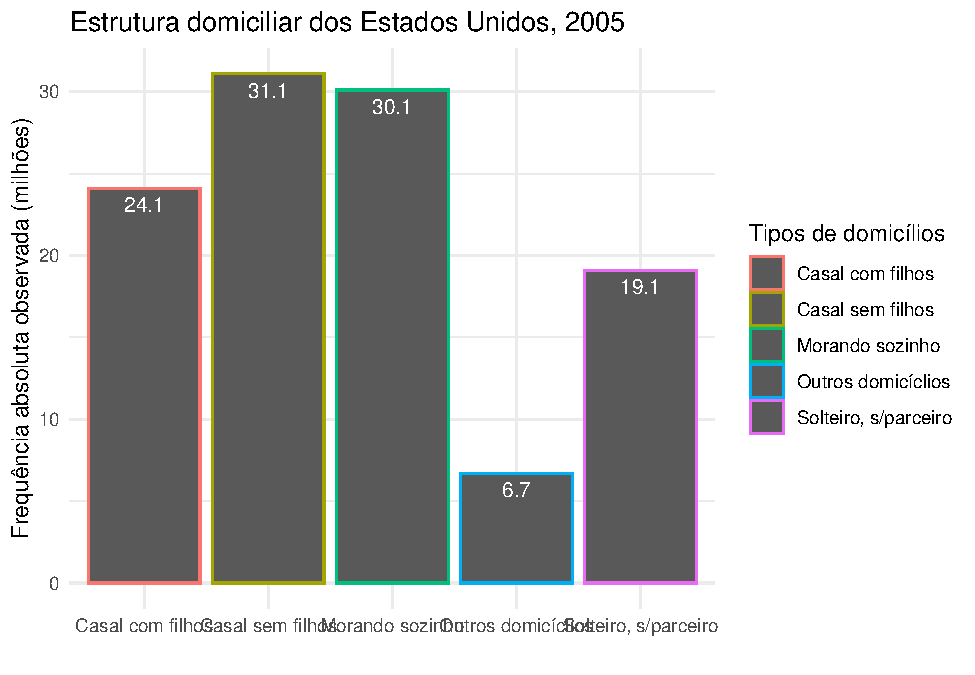
\includegraphics{apostila_files/figure-latex/unnamed-chunk-53-1.pdf}
\caption{\label{fig:unnamed-chunk-53}Gráfico de setores das alturas dos estudantes}
\end{figure}

\hypertarget{box-plot}{%
\subsection{Box-plot}\label{box-plot}}

O gráfico \textbf{Box-plot} ( \emph{box and whisker plot} ): esse gráfico apresenta de modo conjunto, informações sobre a posição, dispersão, assimetria e dados discrepantes do conjunto analisado:

\begin{itemize}
\tightlist
\item
  a mediana (\(q_{2}\));
\item
  os valores mínimo: \(x_{1}\) e máximo: \(x_{n}\) (dados ordenados);
\item
  o 1\(^{o}\) e 3\(^{o}\) quartis;
\item
  a dispersão (intervalo interquartílico: \(q_{3}\) - \(q_{1}\));
\item
  os limites superior: LS= \(q_{3}\) + 1,50\(d_{q}\), e inferior: LI= \(q_{1}\) - 1,50\(d_{q}\) ( \emph{bigodes});
\item
  as observações adjacentes aos limites: situadas entre o 1\(^{o}\) quartil e o LI, e o 3\(^{o}\) quartil e o LS; e,
\item
  as observações exteriores aos limites: situadas abaixo do \emph{LI} ou acima do \emph{LS} que \textbf{podem ou não} ser \emph{outliers} (dados atípicos).
\end{itemize}

\begin{Shaded}
\begin{Highlighting}[]
\NormalTok{res}\OtherTok{=}\FunctionTok{summary}\NormalTok{(y\_normal)}
\NormalTok{min}\OtherTok{=}\NormalTok{res[}\DecValTok{1}\NormalTok{]}
\NormalTok{q1}\OtherTok{=}\NormalTok{res[}\DecValTok{2}\NormalTok{]}
\NormalTok{q2}\OtherTok{=}\NormalTok{res[}\DecValTok{3}\NormalTok{]}
\NormalTok{med}\OtherTok{=}\NormalTok{res[}\DecValTok{4}\NormalTok{]}
\NormalTok{q3}\OtherTok{=}\NormalTok{res[}\DecValTok{5}\NormalTok{]}
\NormalTok{max}\OtherTok{=}\NormalTok{res[}\DecValTok{6}\NormalTok{]}
\NormalTok{dist}\OtherTok{=}\NormalTok{q3}\SpecialCharTok{{-}}\NormalTok{q1}


\FunctionTok{boxplot}\NormalTok{(y\_normal, }\AttributeTok{main=}\StringTok{""}\NormalTok{)}
\FunctionTok{lines}\NormalTok{( }\AttributeTok{y=}\FunctionTok{c}\NormalTok{(min, min), }\AttributeTok{x=}\FunctionTok{c}\NormalTok{(}\FloatTok{0.6}\NormalTok{,}\DecValTok{1}\NormalTok{), }\AttributeTok{col=}\StringTok{"red"}\NormalTok{) }
\FunctionTok{text}\NormalTok{(}\AttributeTok{x=}\FloatTok{0.60}\NormalTok{, }\AttributeTok{y=}\NormalTok{min }\SpecialCharTok{{-}}\FloatTok{0.6}\NormalTok{, }\StringTok{"Primeira observação"}\NormalTok{, }\AttributeTok{col =} \StringTok{"red"}\NormalTok{, }\AttributeTok{srt=}\DecValTok{0}\NormalTok{)}
\FunctionTok{lines}\NormalTok{( }\AttributeTok{y=}\FunctionTok{c}\NormalTok{(max,max), }\AttributeTok{x=}\FunctionTok{c}\NormalTok{(}\FloatTok{0.6}\NormalTok{,}\DecValTok{1}\NormalTok{), }\AttributeTok{col=}\StringTok{"red"}\NormalTok{) }
\FunctionTok{text}\NormalTok{(}\AttributeTok{x=}\FloatTok{0.60}\NormalTok{, }\AttributeTok{y=}\NormalTok{max}\FloatTok{{-}0.6}\NormalTok{, }\StringTok{"Úlitma observação"}\NormalTok{, }\AttributeTok{col =} \StringTok{"red"}\NormalTok{, }\AttributeTok{srt=}\DecValTok{0}\NormalTok{)}
\FunctionTok{lines}\NormalTok{(}\AttributeTok{y=}\FunctionTok{c}\NormalTok{(q2, q2),  }\AttributeTok{x=}\FunctionTok{c}\NormalTok{(}\FloatTok{0.6}\NormalTok{,}\DecValTok{1}\NormalTok{), }\AttributeTok{col=}\StringTok{"red"}\NormalTok{) }
\FunctionTok{text}\NormalTok{(}\AttributeTok{x=}\FloatTok{0.60}\NormalTok{ , }\AttributeTok{y=}\NormalTok{ q2 }\SpecialCharTok{{-}} \FloatTok{0.6}\NormalTok{, }\StringTok{"Mediana"}\NormalTok{, }\AttributeTok{col =} \StringTok{"red"}\NormalTok{, }\AttributeTok{srt=}\DecValTok{0}\NormalTok{)}
\FunctionTok{lines}\NormalTok{(}\AttributeTok{y=}\FunctionTok{c}\NormalTok{(med, med),  }\AttributeTok{x=}\FunctionTok{c}\NormalTok{(}\DecValTok{1}\NormalTok{,}\FloatTok{1.4}\NormalTok{), }\AttributeTok{col=}\StringTok{"red"}\NormalTok{) }
\FunctionTok{text}\NormalTok{(}\AttributeTok{x=}\FloatTok{1.4}\NormalTok{ , }\AttributeTok{y=}\NormalTok{ med }\SpecialCharTok{{-}} \FloatTok{0.6}\NormalTok{, }\StringTok{"Média"}\NormalTok{, }\AttributeTok{col =} \StringTok{"red"}\NormalTok{, }\AttributeTok{srt=}\DecValTok{0}\NormalTok{)}
\FunctionTok{lines}\NormalTok{(}\AttributeTok{y=}\FunctionTok{c}\NormalTok{(q3, q3), }\AttributeTok{x=}\FunctionTok{c}\NormalTok{(}\DecValTok{1}\NormalTok{, }\FloatTok{1.4}\NormalTok{), }\AttributeTok{col=}\StringTok{"red"}\NormalTok{) }
\FunctionTok{text}\NormalTok{(}\AttributeTok{x=} \FloatTok{1.4}\NormalTok{ , }\AttributeTok{y=}\NormalTok{q3 }\SpecialCharTok{{-}} \FloatTok{0.6}\NormalTok{, }\StringTok{"Terceiro Quartil"}\NormalTok{, }\AttributeTok{col =} \StringTok{"red"}\NormalTok{, }\AttributeTok{srt=}\DecValTok{0}\NormalTok{)}
\FunctionTok{lines}\NormalTok{(}\AttributeTok{y=}\FunctionTok{c}\NormalTok{(q1, q1), }\AttributeTok{x=}\FunctionTok{c}\NormalTok{(}\DecValTok{1}\NormalTok{, }\FloatTok{1.4}\NormalTok{), }\AttributeTok{col=}\StringTok{"red"}\NormalTok{) }
\FunctionTok{text}\NormalTok{(}\AttributeTok{x=}\FloatTok{1.4}\NormalTok{, }\AttributeTok{y=}\NormalTok{q1 }\SpecialCharTok{{-}}\FloatTok{0.6}\NormalTok{, }\StringTok{"Primeiro Quartil"}\NormalTok{, }\AttributeTok{col =} \StringTok{"red"}\NormalTok{, }\AttributeTok{srt=}\DecValTok{0}\NormalTok{)}
\FunctionTok{lines}\NormalTok{(}\AttributeTok{y=}\FunctionTok{c}\NormalTok{(q1}\FloatTok{{-}1.5}\SpecialCharTok{*}\NormalTok{dist, q1}\FloatTok{{-}1.5}\SpecialCharTok{*}\NormalTok{dist) , }\AttributeTok{x=}\FunctionTok{c}\NormalTok{(}\DecValTok{1}\NormalTok{,}\FloatTok{1.4}\NormalTok{) , }\AttributeTok{col=}\StringTok{"blue"}\NormalTok{) }
\FunctionTok{text}\NormalTok{(}\AttributeTok{x=}\FloatTok{1.2}\NormalTok{, }\AttributeTok{y=}\NormalTok{q1}\FloatTok{{-}1.5}\SpecialCharTok{*}\NormalTok{dist}\FloatTok{{-}0.6}\NormalTok{ , }\StringTok{"Obs. limitante inferior"}\NormalTok{, }\AttributeTok{col =} \StringTok{"blue"}\NormalTok{, }\AttributeTok{srt=}\DecValTok{0}\NormalTok{)}
\FunctionTok{lines}\NormalTok{(}\AttributeTok{y=}\FunctionTok{c}\NormalTok{(q3}\FloatTok{+1.5}\SpecialCharTok{*}\NormalTok{dist, q3}\FloatTok{+1.5}\SpecialCharTok{*}\NormalTok{dist) , }\AttributeTok{x=}\FunctionTok{c}\NormalTok{(}\DecValTok{1}\NormalTok{,}\FloatTok{1.4}\NormalTok{) , }\AttributeTok{col=}\StringTok{"blue"}\NormalTok{) }
\FunctionTok{text}\NormalTok{(}\AttributeTok{x=}\FloatTok{1.2}\NormalTok{, }\AttributeTok{y=}\NormalTok{q3}\FloatTok{+1.5}\SpecialCharTok{*}\NormalTok{dist }\SpecialCharTok{{-}}\FloatTok{0.6}\NormalTok{ , }\StringTok{"Obs. limitante superior"}\NormalTok{, }\AttributeTok{col =} \StringTok{"blue"}\NormalTok{, }\AttributeTok{srt=}\DecValTok{0}\NormalTok{)}
\end{Highlighting}
\end{Shaded}

\begin{figure}

{\centering 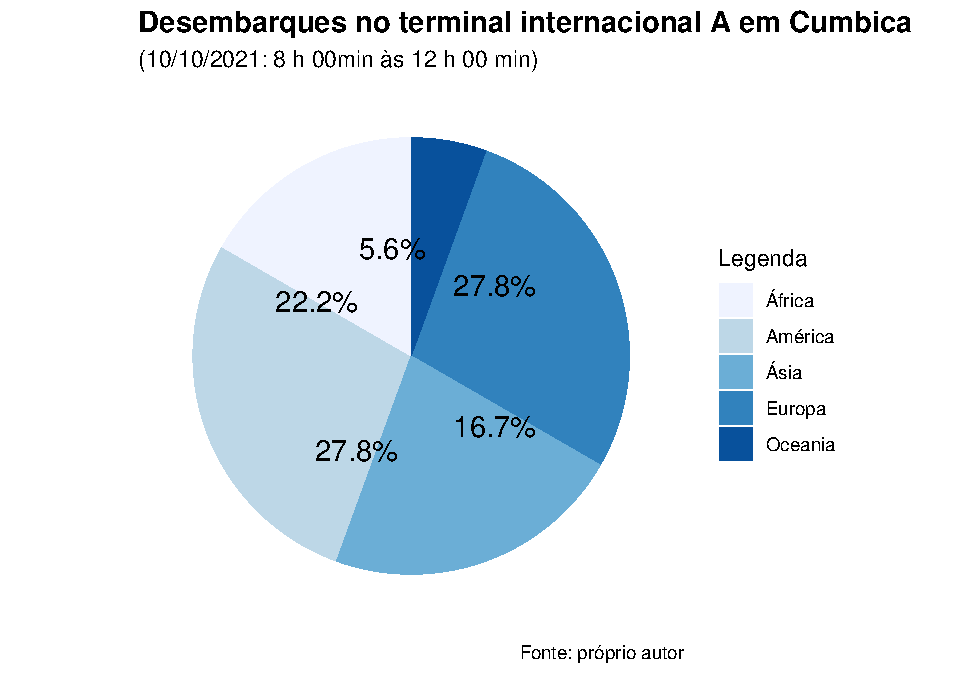
\includegraphics{apostila_files/figure-latex/unnamed-chunk-54-1} 

}

\caption{Box-plot de um rol de valores com Distribuição Normal (média 20 e variãncia 5}\label{fig:unnamed-chunk-54}
\end{figure}

\hypertarget{apresentauxe7uxe3o-tabular-de-dados-quantitativos}{%
\section{Apresentação tabular de dados quantitativos}\label{apresentauxe7uxe3o-tabular-de-dados-quantitativos}}

Ao se lidar com grandes conjuntos de dados a visualização da informação contida nos dados pode ficar comprometida. Um dos modos de se lidar com isso é condensando a informação dos dados brutos em tabelas. Uma tabela é uma forma não discursiva de apresentar informações nas quais o dado numérico se destaca como informação central.

Uma tabela se diferencia de um quadro por este ter todos os seus campos delimitados por linhas e conter apenas informações de natureza qualitativa.

Uma tabela deve ter:

\begin{itemize}
\tightlist
\item
  título que explique o que a tabela contém, local, data;
\item
  cabeçalho com os nomes das variáveis;
\item
  corpo formado pelos dados referentes às variáveis;
\item
  fonte;
\item
  uniformidade no número de casas decimais; e,
\item
  todas as casas devem apresentar valores ou símbolos que expliquem a ausência da informação (NI, NE).
\end{itemize}

Trabalhos de natureza acadêmica ou científica deveriam obrigatoriamente seguir, quando publicados no Brasil, a norma vigente publicada pela ABNT: Associação Brasileira de Normas Técnicas.

Observa-se frequentemente, todavia, que as publicações seguem normas particulares das instituições de ensino (para trabalhos de conclusão de curso, monografias, dissertações e teses) ou das editoras (artigos), muitas vezes mescladas com recomendações da ABNT.

Com o propósito de mostrar alguns gráficos nos exemplos anteriores escolhemos, de modo arbitrário, agrupar seus valores (as alturas) em \emph{classes}.

O procedimento estatístico de agrupar os dados em \emph{classes} ou \emph{categorias} envolve construir uma \emph{tabela de distribuição de frequências}.

Uma \emph{tabela de distribuição de frequências} associa cada \emph{classe} (intervalo) de valores da variável estudada ao número de ocorrências observadas. Como \emph{regra prática}, a repartição dos dados brutos em classes deve sempre observar para que não haja um número excessivo de classes (diminuição da finalidade de resumir os dados, criação de classes sem nenhuma observação) nem tampouco poucas (que não possibilitem a visualização da distribuição e promovam perda da informação original).

A construção de uma \emph{distribuição de frequências} consiste essencialmente em:

\begin{itemize}
\tightlist
\item
  escolher as \emph{classes} ou \emph{intervalos} (dados quantitativos) ou \emph{categorias} (dados qualitativos);
\item
  separar ou enquadrar os dados nessas \emph{classes} ou \emph{categorias}; e,
\item
  contar o número de dados de cada \emph{classe} ou \emph{categoria}.
\end{itemize}

Devemos sempre ter certeza de que cada dado (medida ou observação) se enquadre em uma, e apenas uma, \emph{classe} ou \emph{categoria}.

A literatura propõe vários modos para se determinar o número \emph{k} de classes:

\hfill\break

\begin{longtable}[]{@{}
  >{\raggedright\arraybackslash}p{(\columnwidth - 4\tabcolsep) * \real{0.4384}}
  >{\raggedright\arraybackslash}p{(\columnwidth - 4\tabcolsep) * \real{0.3562}}
  >{\raggedright\arraybackslash}p{(\columnwidth - 4\tabcolsep) * \real{0.2055}}@{}}
\toprule()
\begin{minipage}[b]{\linewidth}\raggedright
Crítério
\end{minipage} & \begin{minipage}[b]{\linewidth}\raggedright
Tamanho da amostra (\emph{n})
\end{minipage} & \begin{minipage}[b]{\linewidth}\raggedright
Fórmula
\end{minipage} \\
\midrule()
\endhead
Raiz quadrada & 25 \(\leq\) n \(\leq\) 220 & k=\(\sqrt{n}\) \\
Herbert \textbf{Sturges} (\emph{log}) & 135 \(\leq\) 572237 & k=1+3,3log(n) \\
Giuseppe \textbf{Milone} (\emph{ln}) & 20 \(\leq 36315\) & k=-1+2ln(n) \\
\bottomrule()
\end{longtable}

\hfill\break

Ao se escolher um número de classes deve-se ponderar para que:

\begin{itemize}
\tightlist
\item
  os intervalos das classes tenham, geralmente, a mesma amplitude;
\item
  os intervalos: do limite inferior da \textbf{primeira classe} ao limite superior da **última classe*, devem conter todos os valores possíveis da variável;
\item
  cada valor observado deve pertencer apenas a uma classe;
\item
  não adotar um número muito elevado de classes de modo que cada classe possua poucas observações (ou mesmo nenhuma); e,
\item
  não adotar um número muito reduzido de classes de modo a esconder a variabilidade dos dados ao se reunir todas as observações em poucas faixas de valores.
\end{itemize}

Em nosso exemplo das alturas dos estudantes, a determinação do número de classes pelo critério da \emph{raiz quadrada} (\emph{n}=60) sugere 8 classes:

\begin{align*}
k & =\sqrt{n} \\
 & = 7,74 \\
 & \sim 8 
\end{align*}

A \emph{amplitude total} (\emph{C}) dos valores observados, \emph{ie}, a diferença entre o \emph{valor máximo} (2,00 m) e o \emph{valor mínimo} (1,41 m) será:

\begin{align*}
C & =2,00-1,41 \\
 & =0,59 m 
\end{align*}

A amplitude de cada uma das classes (\emph{c}) será dada pelo quociente da \emph{amplitude total} (\emph{C}) pelo \emph{número de classes} (\emph{k}).

\hfill\break

\begin{align*}
c & = \frac{C}{k} \\
  & = \frac{0,59}{8}\\ 
  & = 0,07375 m
\end{align*}

A amplitude de cada classe é um valor fracionário que, se adotado, não irá tornar a visualização dos dados mais clara. Mesmo se adotássemos um número imediatamente maior ou menor de classes (\emph{k}=9 ou \emph{k}=7) esse problema persistiria.

Usando bom senso, adotaremos para como intervalo de classe o valor c=0,10 m e a primeira classe começando na altura de 1,40 m.
O total de 6 classes (1,40 m a 2,00 m) cobre toda faixa de variação dos valores dos dados e é de rápida assimilação pelo leitor.

Símbolos gráficos para intervalos:

\begin{itemize}
\tightlist
\item
  Os símbolos abaixo indicam que o valor situado à sua esquerda \textbf{está incluído} no intervalo e o da direita \textbf{não está}:
\end{itemize}

\[
\vdash \\
{\bullet}-{\circ}
\]

\begin{itemize}
\tightlist
\item
  Os símbolos abaixo indicam que o valor situado à sua esquerda \textbf{não está} incluído no intervalo e o da direita **está incluído*:
\end{itemize}

\[
\dashv  \\
{\circ}-{\bullet}
\]

Cada uma das classes terá os seguintes limites inferior e superior:

\hfill\break

1,40 m \(\vdash\) 1,50 m\\
1,50 m \(\vdash\) 1,60 m\\
1,60 m \(\vdash\) 1,70 m\\
1,70 m \(\vdash\) 1,80 m\\
1,80 m \(\vdash\) 1,90 m\\
1,90 m \(\vdash\) 2,00 m

\hfill\break

Veja os dados em rol, onde a cor \textcolor{blue}{azul} indica a mudança de classe com o progredir dos valores das alturas:

\hfill\break

\textcolor{blue}{1,41 ; 1,44 ; 1,47 ;}
1,54 ; 1,55 ; 1,56 ; 1,56 ; 1,56 ; 1,57 ; 1,58 ; 1,58 ;
\textcolor{blue}{1,61 ; 1,62 ; 1,62 ; 1,63 ; 1,64 ;  
1,64 ; 1,65 ; 1,65 ; 1,65 ; 1,65 ; 1,66 ; 1,66 ; 1,66 ; 1,66 ; 1,66 ; 1,67 ; 1,67 ; 1,67 ; 1,67 ; 1,68 ; 1,68 ;  
1,68 ; 1,69 ;}
1,71 ; 1,71 ; 1,72 ; 1,72 ; 1,73 ; 1,73 ; 1,73 ; 1,73 ; 1,73 ; 1,74 ; 1,75 ; 1,76 ; 1,76 ; 1,77 ;\\
1,78 ; 1,78 ;1,79 ; \textcolor{blue}{1,82 ; 1,83 ; 1,83 ; 1,84 ; 1,85 ; 1,86 ; } 1,93 ; 1,95 ; 2,00.\}

\hfill\break

A versão mais simplificada de uma \emph{tabela de distribuição de frequências} (o número de observações nas classes) é de fácil construção, bastando contar o número de observações em cada classe:

\hfill\break

\begin{longtable}[]{@{}ll@{}}
\toprule()
Classe & Frequência (\(n_{i}\)) \\
\midrule()
\endhead
1,40 m \(\vdash\) 1,50 m & 3 \\
1,50 m \(\vdash\) 1,60 m & 8 \\
1,60 m \(\vdash\) 1,70 m & 23 \\
1,70 m \(\vdash\) 1,80 m & 17 \\
1,80 m \(\vdash\) 1,90 m & 6 \\
1,90 m \(\vdash\) 2,00 m & 3 \\
Total & 60 \\
\bottomrule()
\end{longtable}

\hfill\break

\emph{Tabelas de distribuição de frequências} mais completas podem montadas agregando muitas informações adicionais em novas colunas.

Essas informações servem para tornar a visualização mais imediata e muitas delas são obtidas com operações matemáticas elementares:

\hfill\break

\begin{itemize}
\tightlist
\item
  Classe \emph{i}: é a simples identificação de cada classe;
\item
  Amplitude (\(\Delta_{i}\)) da classe \(i\): a diferença entre o valor do limite superior e o do inferior de cada classe;
\item
  Intervalo de valores da classe \(i\) (onde seu limite inferior \textbf{está contido} e o limite superior \textbf{não está contido});
\item
  Valor médio (\(\stackrel{-}{x}_{i}\)) de cada classe \(i\): a média aritmética entre os valores dos limites inferior e superior da classa considerada;
\item
  Frequência absoluta (\(f_{i}\)) da classe \(i\): o número de observações contidas no intervalo da classe considerada;
\item
  Frequência relativa (\(fr_{i}= \frac{f_{i}}{N}\)) da classe \(i\) (ou frequência relativa percentual, se assim apresentada): o quociente do número de observações contidas no intervalo da classe (\(f_{i}\)) pelo número total de observações (\(N\));
\item
  Frequência acumulada (\(fac_{i}\)) da classe \(i\) (ou frequência acumulada percentual, se assim apresentada): o número de observações com medidas contidas na classe \(i\) e nas anteriores a ela;
\item
  Densidade (\(\delta_{i}=\frac{f_{i}}{\Delta_{i}}\)): o quociente do número de observações da classe (\(f_{i}\)) pela sua amplitude (\(\Delta_{i}\));
\item
  Densidade \(\delta_{fr_{i}}=\frac{fr_{i}}{\Delta_{i}}\): o quociente da frequência relativa (\(fr_{i}\)) pela amplitude (\(\Delta_{i}\)) da classe.
\end{itemize}

\hfill\break

Vejo como exemplo as tabelas abaixo:

\hfill\break

\begin{longtable}[]{@{}
  >{\raggedright\arraybackslash}p{(\columnwidth - 14\tabcolsep) * \real{0.0597}}
  >{\raggedright\arraybackslash}p{(\columnwidth - 14\tabcolsep) * \real{0.1567}}
  >{\raggedright\arraybackslash}p{(\columnwidth - 14\tabcolsep) * \real{0.1866}}
  >{\raggedright\arraybackslash}p{(\columnwidth - 14\tabcolsep) * \real{0.0821}}
  >{\raggedright\arraybackslash}p{(\columnwidth - 14\tabcolsep) * \real{0.1194}}
  >{\raggedright\arraybackslash}p{(\columnwidth - 14\tabcolsep) * \real{0.1343}}
  >{\raggedright\arraybackslash}p{(\columnwidth - 14\tabcolsep) * \real{0.1269}}
  >{\raggedright\arraybackslash}p{(\columnwidth - 14\tabcolsep) * \real{0.1343}}@{}}
\toprule()
\begin{minipage}[b]{\linewidth}\raggedright
Classe
\end{minipage} & \begin{minipage}[b]{\linewidth}\raggedright
Int. de valores
\end{minipage} & \begin{minipage}[b]{\linewidth}\raggedright
Alt. média
\end{minipage} & \begin{minipage}[b]{\linewidth}\raggedright
Freq.
\end{minipage} & \begin{minipage}[b]{\linewidth}\raggedright
Freq. relativa
\end{minipage} & \begin{minipage}[b]{\linewidth}\raggedright
Freq. rel. (\%)
\end{minipage} & \begin{minipage}[b]{\linewidth}\raggedright
Freq. acumulada
\end{minipage} & \begin{minipage}[b]{\linewidth}\raggedright
Freq. acum. (\%)
\end{minipage} \\
\midrule()
\endhead
& & (\(\stackrel{-}{x}_{i}\)) & (\(f_{i}\)) & (\(fr_{i}\)) & (\(fr_{i}\%\)) & (\(fac_{i}\)) & (\(fac_{i}\%\)) \\
1 & 1,40 \(\vdash\) 1,50 & 1,45 & 3 & 0,05 & 5 & 3 & 5 \\
2 & 1,50 \(\vdash\) 1,60 & 1,55 & 8 & 0,13 & 13,33 & 11 & 18,33 \\
3 & 1,60 \(\vdash\) 1,70 & 1,65 & 23 & 0,38 & 38,34 & 34 & 56,57 \\
4 & 1,70 \(\vdash\) 1,80 & 1,75 & 17 & 0,28 & 28,33 & 51 & 84,87 \\
5 & 1,80 \(\vdash\) 1,90 & 1,85 & 6 & 0,10 & 10 & 57 & 94,57 \\
6 & 1,90 \(\vdash\) 2,00 & 1,95 & 3 & 0,05 & 5 & 60 & 99,87 \\
Totais & - & & 60 & 1,00 & 100,00 & - & - \\
\bottomrule()
\end{longtable}

\hfill\break

\begin{longtable}[]{@{}
  >{\raggedright\arraybackslash}p{(\columnwidth - 12\tabcolsep) * \real{0.0748}}
  >{\raggedright\arraybackslash}p{(\columnwidth - 12\tabcolsep) * \real{0.1963}}
  >{\raggedright\arraybackslash}p{(\columnwidth - 12\tabcolsep) * \real{0.1028}}
  >{\raggedright\arraybackslash}p{(\columnwidth - 12\tabcolsep) * \real{0.1495}}
  >{\raggedright\arraybackslash}p{(\columnwidth - 12\tabcolsep) * \real{0.1495}}
  >{\raggedright\arraybackslash}p{(\columnwidth - 12\tabcolsep) * \real{0.1121}}
  >{\raggedright\arraybackslash}p{(\columnwidth - 12\tabcolsep) * \real{0.2150}}@{}}
\toprule()
\begin{minipage}[b]{\linewidth}\raggedright
Classe
\end{minipage} & \begin{minipage}[b]{\linewidth}\raggedright
Int. de valores
\end{minipage} & \begin{minipage}[b]{\linewidth}\raggedright
Freq.
\end{minipage} & \begin{minipage}[b]{\linewidth}\raggedright
Amplitude
\end{minipage} & \begin{minipage}[b]{\linewidth}\raggedright
Densidade
\end{minipage} & \begin{minipage}[b]{\linewidth}\raggedright
Freq. rel.
\end{minipage} & \begin{minipage}[b]{\linewidth}\raggedright
Dens. da freq. rel.
\end{minipage} \\
\midrule()
\endhead
& & (\(f_{i}\)) & (\(\Delta_{i}\)) & (\(\delta_{i}\)) & (\(fr_{i}\)) & (\(\delta_{fr_{i}}\)) \\
1 & 1,40 \(\vdash\) 1,50 & 3 & 0,10 & 30 & 0,05 & 0,5 \\
2 & 1,50 \(\vdash\) 1,60 & 8 & 0,10 & 80 & 0,13 & 1,33 \\
3 & 1,60 \(\vdash\) 1,70 & 23 & 0,10 & 230 & 0,39 & 3,83 \\
4 & 1,70 \(\vdash\) 1,80 & 17 & 0,10 & 170 & 0,28 & 2,83 \\
5 & 1,80 \(\vdash\) 1,90 & 6 & 0,10 & 60 & 0,10 & 1 \\
6 & 1,90 \(\vdash\) 2,00 & 3 & 0,10 & 30 & 0,05 & 0,5 \\
Totais & - & 60 & - & - & 1,00 & - \\
\bottomrule()
\end{longtable}

\hfill\break

\hypertarget{muxe9dia-1}{%
\subsection{Média}\label{muxe9dia-1}}

\hfill\break

Nas tabelas de \emph{distribuições de frequências} os resultados estão agrupados em \emph{intervalos de classes (\(i\))}. Por essa razão, os dados perdem sua identidade individual e passam a se representados pelo valor médio de cada intervalo (\(\stackrel{-}{x}_{i}\)).

A média será então dada pelo produto deste valor médio de cada intervalo (\(\stackrel{-}{x}_{i}\)) pela frequência absoluta que ele apresentou (\({n}_{i}\)), dividido pela quantidade de dados (\(N\)).

Sejam \(n_{1}, n_{2}, ..., n_{n}\) as frequências apresentadas para cada intervalo \(i\) dos valores assumidos pela variável \(X\) para o total \(N\) de observações. Assim a \emph{média aritmética simples} para dados agrupados será dada por:

\hfill\break

\[
\stackrel{-}{x}=\frac{\sum _{i=1}^{n}{n}_{i}\cdot{\stackrel{-}{x}}_{i}}{N}
\]\\

\hypertarget{moda-1}{%
\subsection{Moda}\label{moda-1}}

\hfill\break

Moda para dados apresentados na forma de uma distribuição de frequências:

\[
Mo = l_{inf} + (\frac{\Delta_{1}}{\Delta_{1} + \Delta_{2}}) \times \Delta_{i}
\]\\
\strut \\

onde:

\begin{itemize}
\tightlist
\item
  \(l_{inf}\): limite inferior da classe modal, \textbf{a classe de maior frequência absoluta};
\item
  \(\Delta_{1}\) frequência absoluta da \textbf{classe modal} menos a frequência absoluta da \textbf{classe anterior};
\item
  \(\Delta_{2}\) frequência absoluta da \textbf{classe modal} menos a frequência absoluta da \textbf{classe posterior}; e,
\item
  \(\Delta_{i}\) é o intervalo de cada classe.
\end{itemize}

\hypertarget{variuxe2ncia}{%
\subsection{Variância}\label{variuxe2ncia}}

\hfill\break

Variância para dados agrupados:

\[
S^{2}= \frac{1}{n-1} \times \left[  \sum _{i=1}^{n}{(\stackrel{-}{x}}_{i})^{2} \cdot {n}_{i} - \frac{{\left(\sum _{i=1}^{n}{\stackrel{-}{x}}_{i} \cdot {n}_{i}\right)}^{2}  }{n}\right]
\]

Onde:

\begin{itemize}
\tightlist
\item
  \(n_{i}\) é a frequência absoluta em cada classe \(i\); e,
\item
  \(\stackrel{-}{x}_{i}\) é o valor médio de cada classe \(i\).
\end{itemize}

\hypertarget{histograma}{%
\subsection{Histograma}\label{histograma}}

Um \emph{histograma} é a representação gráfica de uma \emph{tabela de distribuição de frequências} em colunas (retângulos).

A base de cada retângulo representa o intervalo de cada classe e a altura, a quantidade ou a \emph{frequência absoluta} com que aquele valor da classe ocorre no conjunto de dados.

O termo \emph{histograma} foi cunhado por Karl Pearson (c.~1891) e vem da composição em grego de \emph{istos} (mastro) com \emph{gramma} (escrita), convertida em inglês para \emph{historical diagram: histogram}.

Como elemento gráfico, seu uso é anterior à sua denominação (maiores detalhes em:
\href{https://www.ine.es/ss/Satellite?blobcol=urldata\&blobheader=application\%2Fpdf\&blobheadername1=Content-Disposition\&blobheadervalue1=attachment\%3B+filename\%3Dart_192_2.pdf\&blobkey=urldata\&blobtable=MungoBlobs\&blobwhere=229\%2F670\%2Fart_192_2.pdf\&ssbinary=true}{(link)} ).

\begin{Shaded}
\begin{Highlighting}[]
\NormalTok{h1}\OtherTok{=}\FunctionTok{hist}\NormalTok{(alturas, }\AttributeTok{breaks=}\FunctionTok{seq}\NormalTok{(}\FloatTok{1.30}\NormalTok{ , }\FloatTok{2.10}\NormalTok{ , }\FloatTok{0.10}\NormalTok{), }\AttributeTok{main=} \StringTok{"Histograma das alturas dos estudantes"}\NormalTok{, }\AttributeTok{col=}\StringTok{"blue"}\NormalTok{, }
\AttributeTok{xlab=}\StringTok{"Classes de altura (m)"}\NormalTok{, }\AttributeTok{ylab=}\StringTok{"Frequência observada (un)"}\NormalTok{ , }\AttributeTok{cex=}\FloatTok{0.7}\NormalTok{, }\AttributeTok{ylim=}\FunctionTok{c}\NormalTok{(}\DecValTok{0}\NormalTok{,}\DecValTok{30}\NormalTok{))}
\FunctionTok{text}\NormalTok{(h1}\SpecialCharTok{$}\NormalTok{mids,h1}\SpecialCharTok{$}\NormalTok{counts,}\AttributeTok{labels=}\NormalTok{h1}\SpecialCharTok{$}\NormalTok{counts, }\AttributeTok{adj=}\FunctionTok{c}\NormalTok{(}\FloatTok{0.5}\NormalTok{, }\SpecialCharTok{{-}}\FloatTok{0.5}\NormalTok{))}
\end{Highlighting}
\end{Shaded}

\begin{figure}
\centering
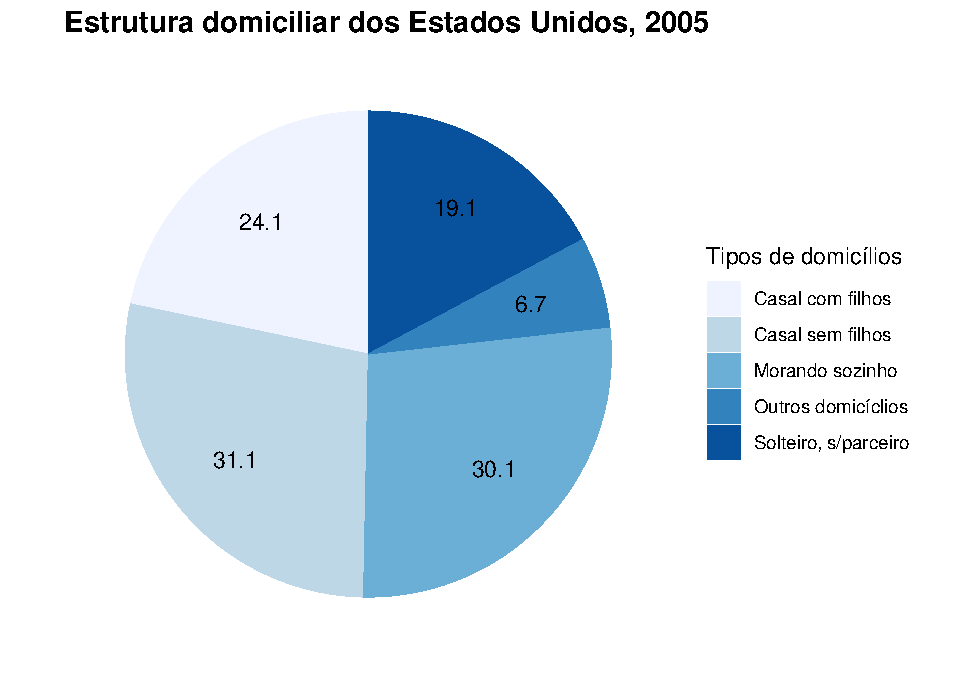
\includegraphics{apostila_files/figure-latex/unnamed-chunk-55-1.pdf}
\caption{\label{fig:unnamed-chunk-55}Histograma das alturas dos estudantes. Uma barra para cada classe de altura e sua altura expressando a quantidade de observações com valores dentro dessa classe (intencionalmente criamos duas classe sem nenhuma observação)}
\end{figure}

As informações da \emph{Tabela de distribuição de frequências} dão origem a variados tipos de histogramas, como aquele feito com as frequências relativas:

\hfill\break

Num histograma de densidade, a altura de cada retângulo representa a densidade da ocorrência da \emph{frequência relativa}.

\begin{Shaded}
\begin{Highlighting}[]
\NormalTok{h2}\OtherTok{=}\FunctionTok{hist}\NormalTok{(alturas,}\AttributeTok{breaks=}\FunctionTok{seq}\NormalTok{(}\FloatTok{1.30}\NormalTok{ , }\FloatTok{2.10}\NormalTok{ , }\FloatTok{0.10}\NormalTok{), }\AttributeTok{main=} \StringTok{"Histograma das alturas dos estudantes"}\NormalTok{, }\AttributeTok{col=}\StringTok{"blue"}\NormalTok{, }
\AttributeTok{xlab=}\StringTok{"Classes de alturas (m)"}\NormalTok{, }\AttributeTok{ylab=}\StringTok{"Frequência relativa observada"}\NormalTok{, }\AttributeTok{prob=}\StringTok{"TRUE"}\NormalTok{, }\AttributeTok{ylim=}\FunctionTok{c}\NormalTok{(}\DecValTok{0}\NormalTok{,}\DecValTok{5}\NormalTok{))}
\FunctionTok{text}\NormalTok{(h2}\SpecialCharTok{$}\NormalTok{mids,h2}\SpecialCharTok{$}\NormalTok{density,}\AttributeTok{labels=}\FunctionTok{round}\NormalTok{(h2}\SpecialCharTok{$}\NormalTok{density, }\DecValTok{5}\NormalTok{), }\AttributeTok{adj=}\FunctionTok{c}\NormalTok{(}\FloatTok{0.5}\NormalTok{, }\SpecialCharTok{{-}}\FloatTok{0.5}\NormalTok{), }\AttributeTok{cex=}\FloatTok{0.7}\NormalTok{)}
\FunctionTok{lines}\NormalTok{(}\FunctionTok{density}\NormalTok{(alturas), }\AttributeTok{col=}\StringTok{"red"}\NormalTok{)             }
\FunctionTok{lines}\NormalTok{(}\FunctionTok{density}\NormalTok{(alturas, }\AttributeTok{adjust=}\DecValTok{2}\NormalTok{), }\AttributeTok{lty=}\StringTok{"dotted"}\NormalTok{)  }
\end{Highlighting}
\end{Shaded}

\begin{figure}
\centering
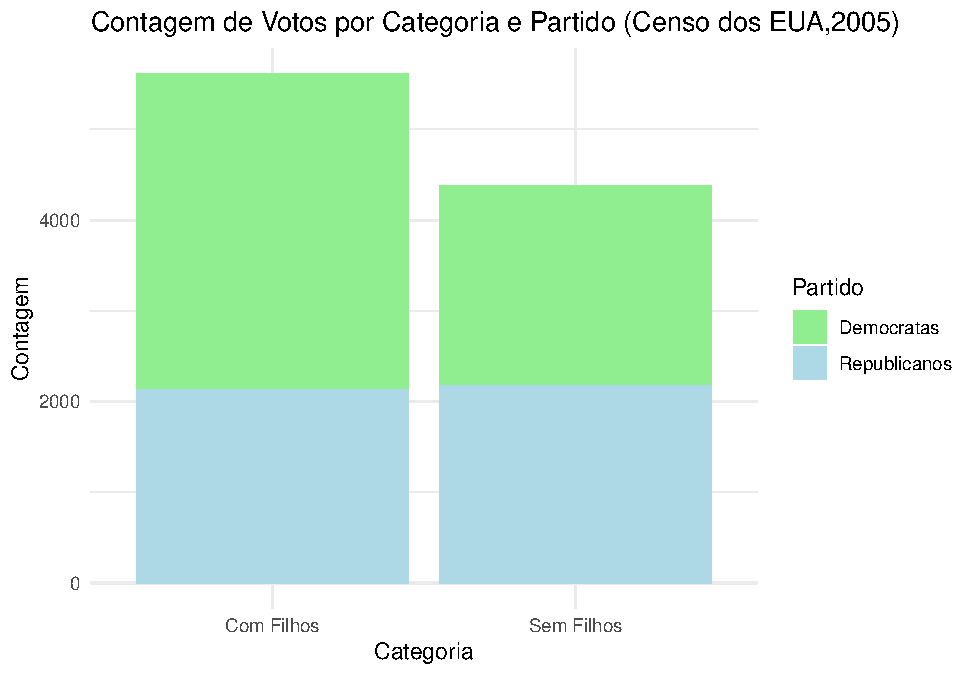
\includegraphics{apostila_files/figure-latex/unnamed-chunk-56-1.pdf}
\caption{\label{fig:unnamed-chunk-56}A linha vermelha é uma aproximação da Função de Densidade da frequência relativa de observação (a linhe preta é a curva da função densidade de uma distribuição Normal com média e variâncias dadas pelos dados}
\end{figure}

\hfill\break

Uma aproximação para a \textbf{área sob a curva da Função de Densidade} pode ser soma das áreas de cada retângulo, onde cada um deles tem:

\begin{itemize}
\tightlist
\item
  Base = \(\Delta_{i}\); e,\textbackslash{}
\item
  Altura = Densidade da proporção= \(\frac{f_{i}}{\Delta_{i}}\).
\end{itemize}

Portanto, a área de cada retângulo é igual à proporção (\(f_{i}\)) da classe (\(i\)) e, assim, a soma de todas essas áreas será igual a 1:

\hfill\break

\begin{Shaded}
\begin{Highlighting}[]
\NormalTok{(}\FloatTok{0.10}\SpecialCharTok{*}\FloatTok{0.5}\NormalTok{)}\SpecialCharTok{+}\NormalTok{(}\FloatTok{0.10}\SpecialCharTok{*}\FloatTok{1.333}\NormalTok{)}\SpecialCharTok{+}\NormalTok{(}\FloatTok{0.10}\SpecialCharTok{*}\FloatTok{3.833}\NormalTok{)}\SpecialCharTok{+}\NormalTok{(}\FloatTok{0.10}\SpecialCharTok{*}\FloatTok{2.833}\NormalTok{)}\SpecialCharTok{+}\NormalTok{(}\FloatTok{0.10}\SpecialCharTok{*}\DecValTok{1}\NormalTok{)}\SpecialCharTok{+}\NormalTok{(}\FloatTok{0.10}\SpecialCharTok{*}\FloatTok{0.50}\NormalTok{)}
\end{Highlighting}
\end{Shaded}

\begin{verbatim}
## [1] 0.9999
\end{verbatim}

\hfill\break

A \textbf{área da curva da Função de Densidade delimitada por dois valores quaisquer} é uma analogia para a probabilidade de que um determinado valor de altura de um estudante (amostrado aleatoriamente dentre todos os 60 estudantes) esteja contida nesse intervalo.

\textbf{Equivale dizer que}, amostrando-se aleatoriamente um estudante dentre todos os 60 alunos, a probabilidade de que a altura desse estudante estaje contida entre os valores mínimo e máximo da amostra é, \textbf{naturalmente}, igual a 1 (100\%)

\hfill\break

\hypertarget{apresentauxe7uxe3o-tabular-de-dados-qualitativos}{%
\section{Apresentação tabular de dados qualitativos}\label{apresentauxe7uxe3o-tabular-de-dados-qualitativos}}

Frequentemente pesquisas são conduzidas tendo por base respostas de natureza binária como, por exemplo:

\begin{itemize}
\tightlist
\item
  sim ou não;
\item
  gosto ou não gosto;
\item
  voto em ``A'' ou voto em ``B''; ou,
\item
  concordo ou não concordo.
\end{itemize}

Como resultado final, são obtidas proporções que expressam a frequência absoluta com que cada uma dessas variáveis (ou seus níveis) foi observada em relação ao total estudado.

Para essas situações, variados tipos de apresentações tabulares podem ser produzidos como a tabela abaixo, onde são apresentadas as proporções observadas de cada nível da variável estudada (``tipo de família'', com quatro níveis diferentes), de um levantamento amostral feito pela Agência do Censo dos Estados Unidos em 2005.

\hfill\break

\begin{longtable}[]{@{}
  >{\raggedright\arraybackslash}p{(\columnwidth - 6\tabcolsep) * \real{0.3333}}
  >{\raggedright\arraybackslash}p{(\columnwidth - 6\tabcolsep) * \real{0.2500}}
  >{\raggedright\arraybackslash}p{(\columnwidth - 6\tabcolsep) * \real{0.1667}}
  >{\raggedright\arraybackslash}p{(\columnwidth - 6\tabcolsep) * \real{0.2500}}@{}}
\toprule()
\begin{minipage}[b]{\linewidth}\raggedright
Tipo de família
\end{minipage} & \begin{minipage}[b]{\linewidth}\raggedright
Número (milhões)
\end{minipage} & \begin{minipage}[b]{\linewidth}\raggedright
Freq. abs.
\end{minipage} & \begin{minipage}[b]{\linewidth}\raggedright
Freq. rel. (\%)
\end{minipage} \\
\midrule()
\endhead
Casal com filhos & 24,1 & 0,22 & 22 \\
Casal sem filhos & 31,1 & 0,28 & 28 \\
Solteiro, sem parceiro & 19,1 & 0,17 & 17 \\
Morando sozinho & 30,1 & 0,27 & 27 \\
Outros domicílios & 6,7 & 0,06 & 6 \\
\bottomrule()
\end{longtable}

A apresentação gráfica desses dados pode feita, por exemplo, por um \emph{Gráfico de colunas} ou um \emph{Gráfico de setores}.

\hfill\break

\begin{Shaded}
\begin{Highlighting}[]
\FunctionTok{library}\NormalTok{(ggplot2)}
\NormalTok{dados}\OtherTok{=}\FunctionTok{data.frame}\NormalTok{(}\AttributeTok{tipo=}\FunctionTok{c}\NormalTok{(}\StringTok{"Casal com filhos"}\NormalTok{,}
                          \StringTok{"Casal sem filhos"}\NormalTok{,}
                          \StringTok{"Solteiro, s/parceiro"}\NormalTok{,}
                          \StringTok{"Morando sozinho"}\NormalTok{,}
                          \StringTok{"Outros domicíclios"}\NormalTok{),}
                 \AttributeTok{quant=}\FunctionTok{c}\NormalTok{(}\FloatTok{24.1}\NormalTok{, }\FloatTok{31.1}\NormalTok{, }
                       \FloatTok{19.1}\NormalTok{, }\FloatTok{30.1}\NormalTok{,}
                       \FloatTok{6.7}\NormalTok{))}

\FunctionTok{ggplot}\NormalTok{(dados, }\FunctionTok{aes}\NormalTok{(}\AttributeTok{x=}\NormalTok{tipo, }\AttributeTok{y=}\NormalTok{quant, }\AttributeTok{color=}\NormalTok{tipo)) }\SpecialCharTok{+}
\FunctionTok{geom\_bar}\NormalTok{(}\AttributeTok{stat=}\StringTok{"identity"}\NormalTok{, }\AttributeTok{position=}\FunctionTok{position\_dodge}\NormalTok{())}\SpecialCharTok{+}
\FunctionTok{ggtitle}\NormalTok{(}\StringTok{"Estrutura domiciliar dos Estados Unidos, 2005"}\NormalTok{) }\SpecialCharTok{+}
\FunctionTok{theme}\NormalTok{(}\AttributeTok{legend.position=}\StringTok{"bottom"}\NormalTok{)}\SpecialCharTok{+}
\FunctionTok{geom\_text}\NormalTok{(}\FunctionTok{aes}\NormalTok{(}\AttributeTok{label=}\NormalTok{quant), }\AttributeTok{vjust=}\FloatTok{1.6}\NormalTok{, }\AttributeTok{color=}\StringTok{"white"}\NormalTok{, }\AttributeTok{position =} \FunctionTok{position\_dodge}\NormalTok{(}\FloatTok{0.9}\NormalTok{), }\AttributeTok{size=}\FloatTok{3.5}\NormalTok{)}\SpecialCharTok{+}
\FunctionTok{scale\_fill\_brewer}\NormalTok{(}\AttributeTok{palette=}\StringTok{"Paired"}\NormalTok{)}\SpecialCharTok{+}
\FunctionTok{theme\_minimal}\NormalTok{()}\SpecialCharTok{+}
\FunctionTok{xlab}\NormalTok{(}\StringTok{""}\NormalTok{)  }\SpecialCharTok{+}
\FunctionTok{ylab}\NormalTok{(}\StringTok{"Frequência absoluta observada (milhões)"}\NormalTok{)}\SpecialCharTok{+}
\FunctionTok{labs}\NormalTok{(}\AttributeTok{colour =} \StringTok{"Tipos de domicílios"}\NormalTok{) }
\end{Highlighting}
\end{Shaded}

\begin{figure}
\centering
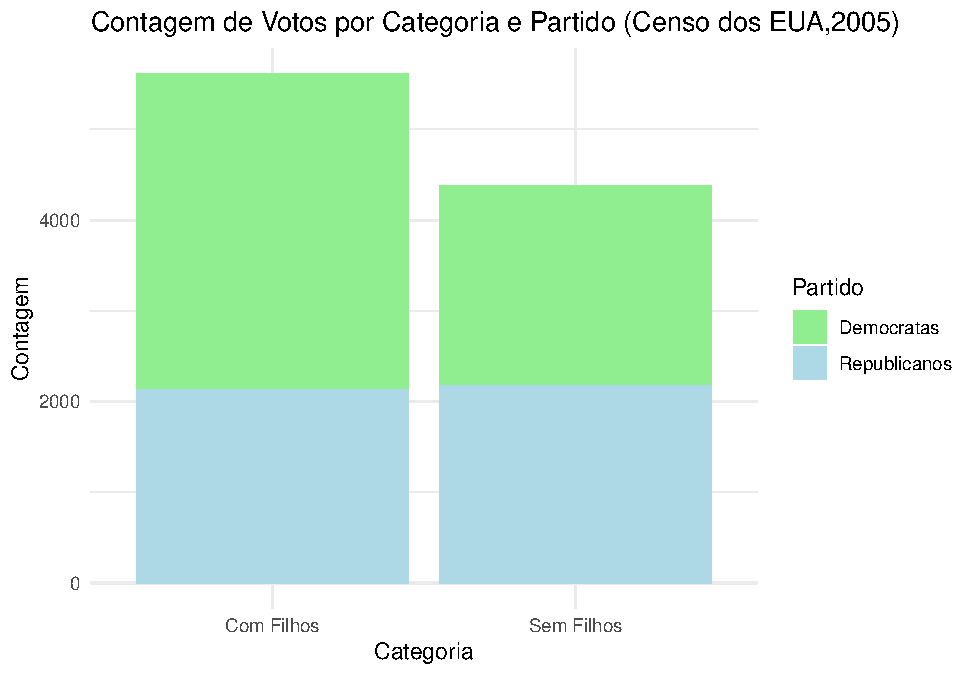
\includegraphics{apostila_files/figure-latex/unnamed-chunk-58-1.pdf}
\caption{\label{fig:unnamed-chunk-58}Gráfico de barras}
\end{figure}

\hfill\break

\begin{Shaded}
\begin{Highlighting}[]
\FunctionTok{library}\NormalTok{(ggplot2)}
\FunctionTok{library}\NormalTok{(scales)}

\NormalTok{blank\_theme}\OtherTok{=}\FunctionTok{theme\_minimal}\NormalTok{()}\SpecialCharTok{+}
  \FunctionTok{theme}\NormalTok{(}
    \AttributeTok{axis.title.x =} \FunctionTok{element\_blank}\NormalTok{(),}
    \AttributeTok{axis.title.y =} \FunctionTok{element\_blank}\NormalTok{(),}
    \AttributeTok{panel.border =} \FunctionTok{element\_blank}\NormalTok{(),}
    \AttributeTok{panel.grid=}\FunctionTok{element\_blank}\NormalTok{(),}
    \AttributeTok{axis.ticks =} \FunctionTok{element\_blank}\NormalTok{(),}
    \AttributeTok{plot.title=}\FunctionTok{element\_text}\NormalTok{(}\AttributeTok{size=}\DecValTok{14}\NormalTok{, }\AttributeTok{face=}\StringTok{"bold"}\NormalTok{)}
\NormalTok{  )}

\NormalTok{bp}\OtherTok{=}\FunctionTok{ggplot}\NormalTok{(dados, }\FunctionTok{aes}\NormalTok{(}\AttributeTok{x=}\StringTok{""}\NormalTok{, }\AttributeTok{y=}\NormalTok{quant, }\AttributeTok{fill=}\NormalTok{tipo))}\SpecialCharTok{+}
  \FunctionTok{geom\_bar}\NormalTok{(}\AttributeTok{width =} \DecValTok{1}\NormalTok{, }\AttributeTok{stat =} \StringTok{"identity"}\NormalTok{)}
\NormalTok{pie}\OtherTok{=}\NormalTok{bp }\SpecialCharTok{+} \FunctionTok{coord\_polar}\NormalTok{(}\StringTok{"y"}\NormalTok{, }\AttributeTok{start=}\DecValTok{0}\NormalTok{)}
\NormalTok{pie }\SpecialCharTok{+} 
  \FunctionTok{scale\_fill\_brewer}\NormalTok{(}\StringTok{"Blues"}\NormalTok{)}\SpecialCharTok{+}
\NormalTok{  blank\_theme }\SpecialCharTok{+}
  \FunctionTok{theme}\NormalTok{(}\AttributeTok{axis.text.x=}\FunctionTok{element\_blank}\NormalTok{()) }\SpecialCharTok{+}
  \FunctionTok{geom\_text}\NormalTok{(}\FunctionTok{aes}\NormalTok{(}\AttributeTok{x =}  \FloatTok{1.2}\NormalTok{,}\AttributeTok{label =}\NormalTok{ quant), }\AttributeTok{position =} \FunctionTok{position\_stack}\NormalTok{(}\AttributeTok{vjust =} \FloatTok{0.5}\NormalTok{)) }\SpecialCharTok{+}
  \FunctionTok{ggtitle}\NormalTok{(}\StringTok{"Estrutura domiciliar dos Estados Unidos, 2005"}\NormalTok{) }\SpecialCharTok{+}
  \FunctionTok{theme}\NormalTok{(}\AttributeTok{legend.position =} \StringTok{"right"}\NormalTok{, }\AttributeTok{legend.justification =} \StringTok{"center"}\NormalTok{, }\AttributeTok{legend.direction =} \StringTok{"vertical"}\NormalTok{,}
        \AttributeTok{legend.spacing.x =} \FunctionTok{unit}\NormalTok{(}\FloatTok{0.5}\NormalTok{, }\StringTok{\textquotesingle{}cm\textquotesingle{}}\NormalTok{),}\AttributeTok{legend.spacing.y =} \FunctionTok{unit}\NormalTok{(}\FloatTok{0.5}\NormalTok{, }\StringTok{\textquotesingle{}cm\textquotesingle{}}\NormalTok{))}\SpecialCharTok{+}
  \FunctionTok{guides}\NormalTok{(}\AttributeTok{fill =} \FunctionTok{guide\_legend}\NormalTok{(}\AttributeTok{title =} \StringTok{"Tipos de domicílios"}\NormalTok{,}
                             \AttributeTok{label.position =} \StringTok{"right"}\NormalTok{,}
                             \AttributeTok{title.position =} \StringTok{"top"}\NormalTok{, }\AttributeTok{title.vjust =} \DecValTok{1}\NormalTok{)) }
\end{Highlighting}
\end{Shaded}

\begin{figure}
\centering
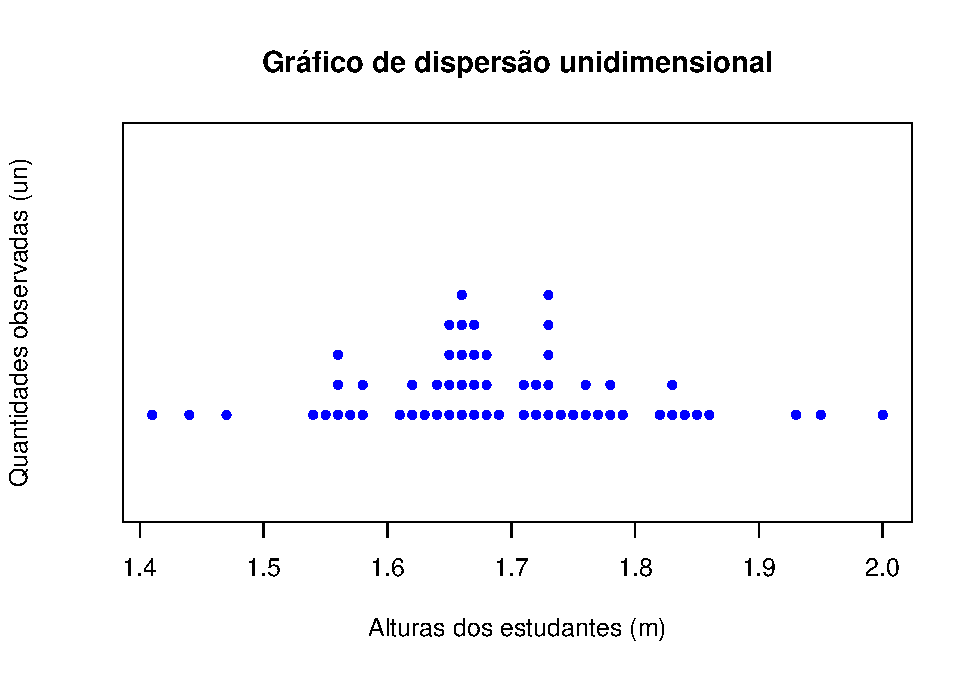
\includegraphics{apostila_files/figure-latex/unnamed-chunk-59-1.pdf}
\caption{\label{fig:unnamed-chunk-59}Gráfico de setores}
\end{figure}

\hfill\break

Outro tipo de apresentação tabular de dados qualitativos são as \emph{Tabelas de Contingência}.

As tabelas de contingência são usadas para associar duas ou mais variáveis qualitativas (ou seus níveis) às respostas obtidas, na forma das frequências absoluta e relativa observadas em cada uma dessas variáveis (ou seus níveis).

O uso desse tipo de tabela é comum quando se pretende investigar se as variáveis estudadas têm alguma associação por meio de testes não paramétricos. Esse tipo de apresentação facilita a extração de informações relacionadas às probabilidades marginais ou condicionadas de cada uma variáveis ou seus níveis.

\hfill\break

\begin{longtable}[]{@{}
  >{\raggedright\arraybackslash}p{(\columnwidth - 4\tabcolsep) * \real{0.3594}}
  >{\raggedright\arraybackslash}p{(\columnwidth - 4\tabcolsep) * \real{0.3125}}
  >{\raggedright\arraybackslash}p{(\columnwidth - 4\tabcolsep) * \real{0.3281}}@{}}
\toprule()
\begin{minipage}[b]{\linewidth}\raggedright
Inclinação partidária
\end{minipage} & \begin{minipage}[b]{\linewidth}\raggedright
\end{minipage} & \begin{minipage}[b]{\linewidth}\raggedright
\end{minipage} \\
\midrule()
\endhead
& Democrata & Republicano \\
Casal com filhos & 762 & 468 \\
Casal sem filhos & 484 & 477 \\
Total & 1246 & 945 \\
----------------------- & -------------------- & --------------------- \\
\bottomrule()
\end{longtable}

\hfill\break

\begin{longtable}[]{@{}
  >{\raggedright\arraybackslash}p{(\columnwidth - 6\tabcolsep) * \real{0.2614}}
  >{\raggedright\arraybackslash}p{(\columnwidth - 6\tabcolsep) * \real{0.2841}}
  >{\raggedright\arraybackslash}p{(\columnwidth - 6\tabcolsep) * \real{0.2614}}
  >{\raggedright\arraybackslash}p{(\columnwidth - 6\tabcolsep) * \real{0.1932}}@{}}
\toprule()
\begin{minipage}[b]{\linewidth}\raggedright
Inclinação partidária
\end{minipage} & \begin{minipage}[b]{\linewidth}\raggedright
\end{minipage} & \begin{minipage}[b]{\linewidth}\raggedright
\end{minipage} & \begin{minipage}[b]{\linewidth}\raggedright
\end{minipage} \\
\midrule()
\endhead
& Democrata (milhões) & Republicano (milhões) & Total (milhões) \\
Casal com filhos & 18,0 & 6,1 & 24,1 \\
Casal sem filhos & 29,1 & 2,0 & 31,1 \\
Total & 47,1 & 8,1 & 55,2 \\
\bottomrule()
\end{longtable}

As representações gráficas são análogas às mostradas no exemplo anterior.

\hypertarget{probabilidade}{%
\chapter{- Introdução ao cálculo de probabilidades}\label{probabilidade}}

\begin{quote}
\_``Not everything that can be counted counts and not everything that counts can be counted {[}\ldots{]}'' (Albert Einstein, 1879-1955)
\end{quote}

Seria bom começar um curso sobre teoria das probabilidades, dando uma definição de probabilidade concisa, simples e intuitiva, mas rigorosa. Infelizmente, isto não será possível.

Se por um lado, uma definição rigorosa de probabilidade requer um aparato matemático sofisticado e é bem pouco intuitiva; por outro lado, definições simples são frequentemente enganosas ou, na melhor das hipóteses, tautológicas .

Por exemplo, poderíamos dizer que probabilidade:

\begin{quote}
é um \emph{número} que quantifica, uma \emph{medida da informação} disponível sobre a possibilidade de ocorrência de um determinado \emph{evento} quando ainda não se sabe se ele ocorrerá ou não.
\end{quote}

Essa definição é circular (\emph{definiendum=definien} porque usa o conceito de probabilidade, que é um sinônimo de possibilidade, chance, esperança, viabilidade, exequibilidade, expectativa, \dots).

Todavia ela nos introduz \textbf{dois conceitos} que iremos usar como ponto de partida:

\begin{enumerate}
\def\labelenumi{\arabic{enumi}.}
\tightlist
\item
  probabilidade refere-se a \emph{experimentos aleatórios} e seus \emph{eventos}; e,
\item
  probabilidade é um \emph{número}.
\end{enumerate}

O \emph{conceito clássico} de probabilidade será a seguir apresentado e, ao final será abordado o conceito de probabilidade como uma função matemática alicerçada em alguns postulados (\emph{conceito axiomático}).

\hypertarget{introduuxe7uxe3o-conceitual-essencial}{%
\section{Introdução conceitual essencial}\label{introduuxe7uxe3o-conceitual-essencial}}

\hfill\break

\hypertarget{experimentos-determinuxedsticos-e-experimentos-probabiluxedsticos-aleatuxf3rios}{%
\subsection{Experimentos determinísticos e experimentos probabilísticos (aleatórios)}\label{experimentos-determinuxedsticos-e-experimentos-probabiluxedsticos-aleatuxf3rios}}

\hfill\break

Aleatório provem do latim: \emph{aleatorium}: fato cujo desfecho depende de um acontecimento futuro e incerto, resultado da sorte ou acaso, acidental.

\hfill\break

Ao contrário de um \textbf{experimento determinístico}, cujo resultado pode ser previamente determinado (como a reação de dois átomos de \emph{H} com um átomo de \emph{O} ou a distância percorrida - no vácuo sob velocidade constante e sem atrito - por um objeto \(S = V \times t\)), o conceito de experimento aleatório é o que estabelece que seu resultado \textbf{não pode ser previsto com certeza}.

Os resultados observados \textbf{apresentam variações} mesmo quando esses experimentos são repetidos indefinidamente e sob as mesmas condições; todavia, é possível estabelecer um conjunto cujos elementos compõem todos os possíveis resultados.

\hypertarget{espauxe7o-amostral-e-seus-elementos}{%
\subsection{Espaço amostral e seus elementos}\label{espauxe7o-amostral-e-seus-elementos}}

\hfill\break
A primeira coisa que fazemos quando começamos a pensar sobre a probabilidade de ocorrência de um certo resultado em um \textbf{experimento aleatório} é listar \textbf{todos os resultados com possibilidade de ocorrência}.

Esses resultados são os elementos de um conjunto a que denominamos de \emph{espaço amostral} e, usualmente o representamos pela letra grega maiúscula \(\Omega\).

Para que \(\Omega\) seja considerado o \emph{espaço amostral} desse experimento aleatório ele precisa apresentar duas propriedades:

1- \textbf{apenas um} de seus elementos pode ocorrer ao se realizar o \emph{experimento aleatório} (\textbf{resultado}); e,
2- \textbf{ao menos um} dos possíveis resultados deverá ocorrer.

Tais propriedades são equivalentes a se dizer que os elementos do espaço amostral, os \textbf{resultados}listados como possibilidades de se verificar ao se realizar um \textbf{experimento aleatório} são \textbf{mutuamente exclusivos e exaustivos}.

Exemplos clássicos de experimentos aleatórios são o \emph{lançamento de moedas}, \emph{dados} ou extração de \emph{cartas de um baralho}.

Os possíveis resultados como a face de uma moeda ou o número que um dado irá expor ao ser lançado, \textbf{embora não possam ser antecipados com certeza}, encontram-se limitados a um conjunto de todas as uas possibilidades, seu \textbf{espaço amostral}.

Para o lançamento de um dado:

\[
\Omega = \{ 1,2,3,4,5,6\}
\]

e para o lançamento de uma moeda

\[\Omega=\{\text{cara}, \text{coroa}\}
\].

Um espaço amostral consiste então da enumeração (finita ou infinita) de todos os resultados possíveis de serem gerados em um experimento aleatório, generalizado como sendo o conjunto

\[
\Omega = \{\omega_{1}, \omega_{2}, \omega_{3}, ..., \omega_{n}, \dots \}
\]

\textbf{Cada um} dos possíveis resultados de um experimento aleatório com espaço amostral \(\Omega\) é chamado de um \textbf{elemento} desse espaço amostral e é denotado pela letra grega: \(\omega_{n}\).

\hypertarget{evento-de-interesse-sucesso}{%
\subsection{Evento de interesse (sucesso)}\label{evento-de-interesse-sucesso}}

\hfill\break

\hypertarget{evento}{%
\subsection{Evento}\label{evento}}

\hfill\break

Denomina-se como \textbf{evento} um \textbf{subconjunto} finito do \textbf{espaço amostral} composto por um ou mais de seus elementos, e que \textbf{satisfazem (atendem)} ao enunciado definido no experimento aleatório desejado.

A expressão \textbf{evento de interesse} (ou sucesso) define, para o cálculo de probabilidades, a ocorrência de um resultado previamente definido no experimento aleatório.

Admita um \textbf{experimento aleatório} que consiste em se lançar um dado uma vez. Um \textbf{evento de interesse} pode ser definido como sendo obter um número par. A partir dessas condições, pode-se calcular-se a probabilidade de se obter \textbf{sucesso} no experimento aleatório; isto é, obter-se um número par ao se lançar um dado uma vez.

Admita umoutro experimento aleatório que agora consiste em se lançar uma moeda duas vezes.

O \textbf{espaço amostral} desse experimento aleatório (\textbf{todos os possíveis resultados}) será um conjunto composto por quatro elementos:

\[
\Omega = \{\omega_{1}, \omega_{2}, \omega_{3}, \omega_{4}\}
\]

onde:

\begin{align*}
\omega_{1} & = (\text{Cara}, \text{Coroa})\\
\omega_{2} & = (\text{Coroa}, \text{Cara})\\
\omega_{3} & = (\text{Cara}, \text{Cara}) \\
\omega_{4} & = (\text{Coroa}, \text{Coroa})
\end{align*}

Se definirmos como \textbf{sucesso} nesse experimento aleatório obter-se

\[
E=\{(Cara, Cara)\}
\],

dizemos que \(E\) é um \textbf{evento simples} pois é formado por apenas \textbf{um} elemento do espaço amostral.

Por outro lado, se definimos nosso sucesso como sendo obter

\[
E_{1}=\{(Cara, Coroa) ou (Coroa, Cara)\}
\]

\(E_{1}\) será um \textbf{evento composto} pois é formado por \textbf{dois} elementos do espaço amostral.

Se codificarmos \textbf{Cara: 1} e \textbf{Coroa: 0}, podemos representar simultaneamente o espaço amostral \(\Omega\) do experimento aleatório e o **evento de sucesso* \(E_{1}\) de modo grafico.

\hfill\break

\begin{figure}

{\centering 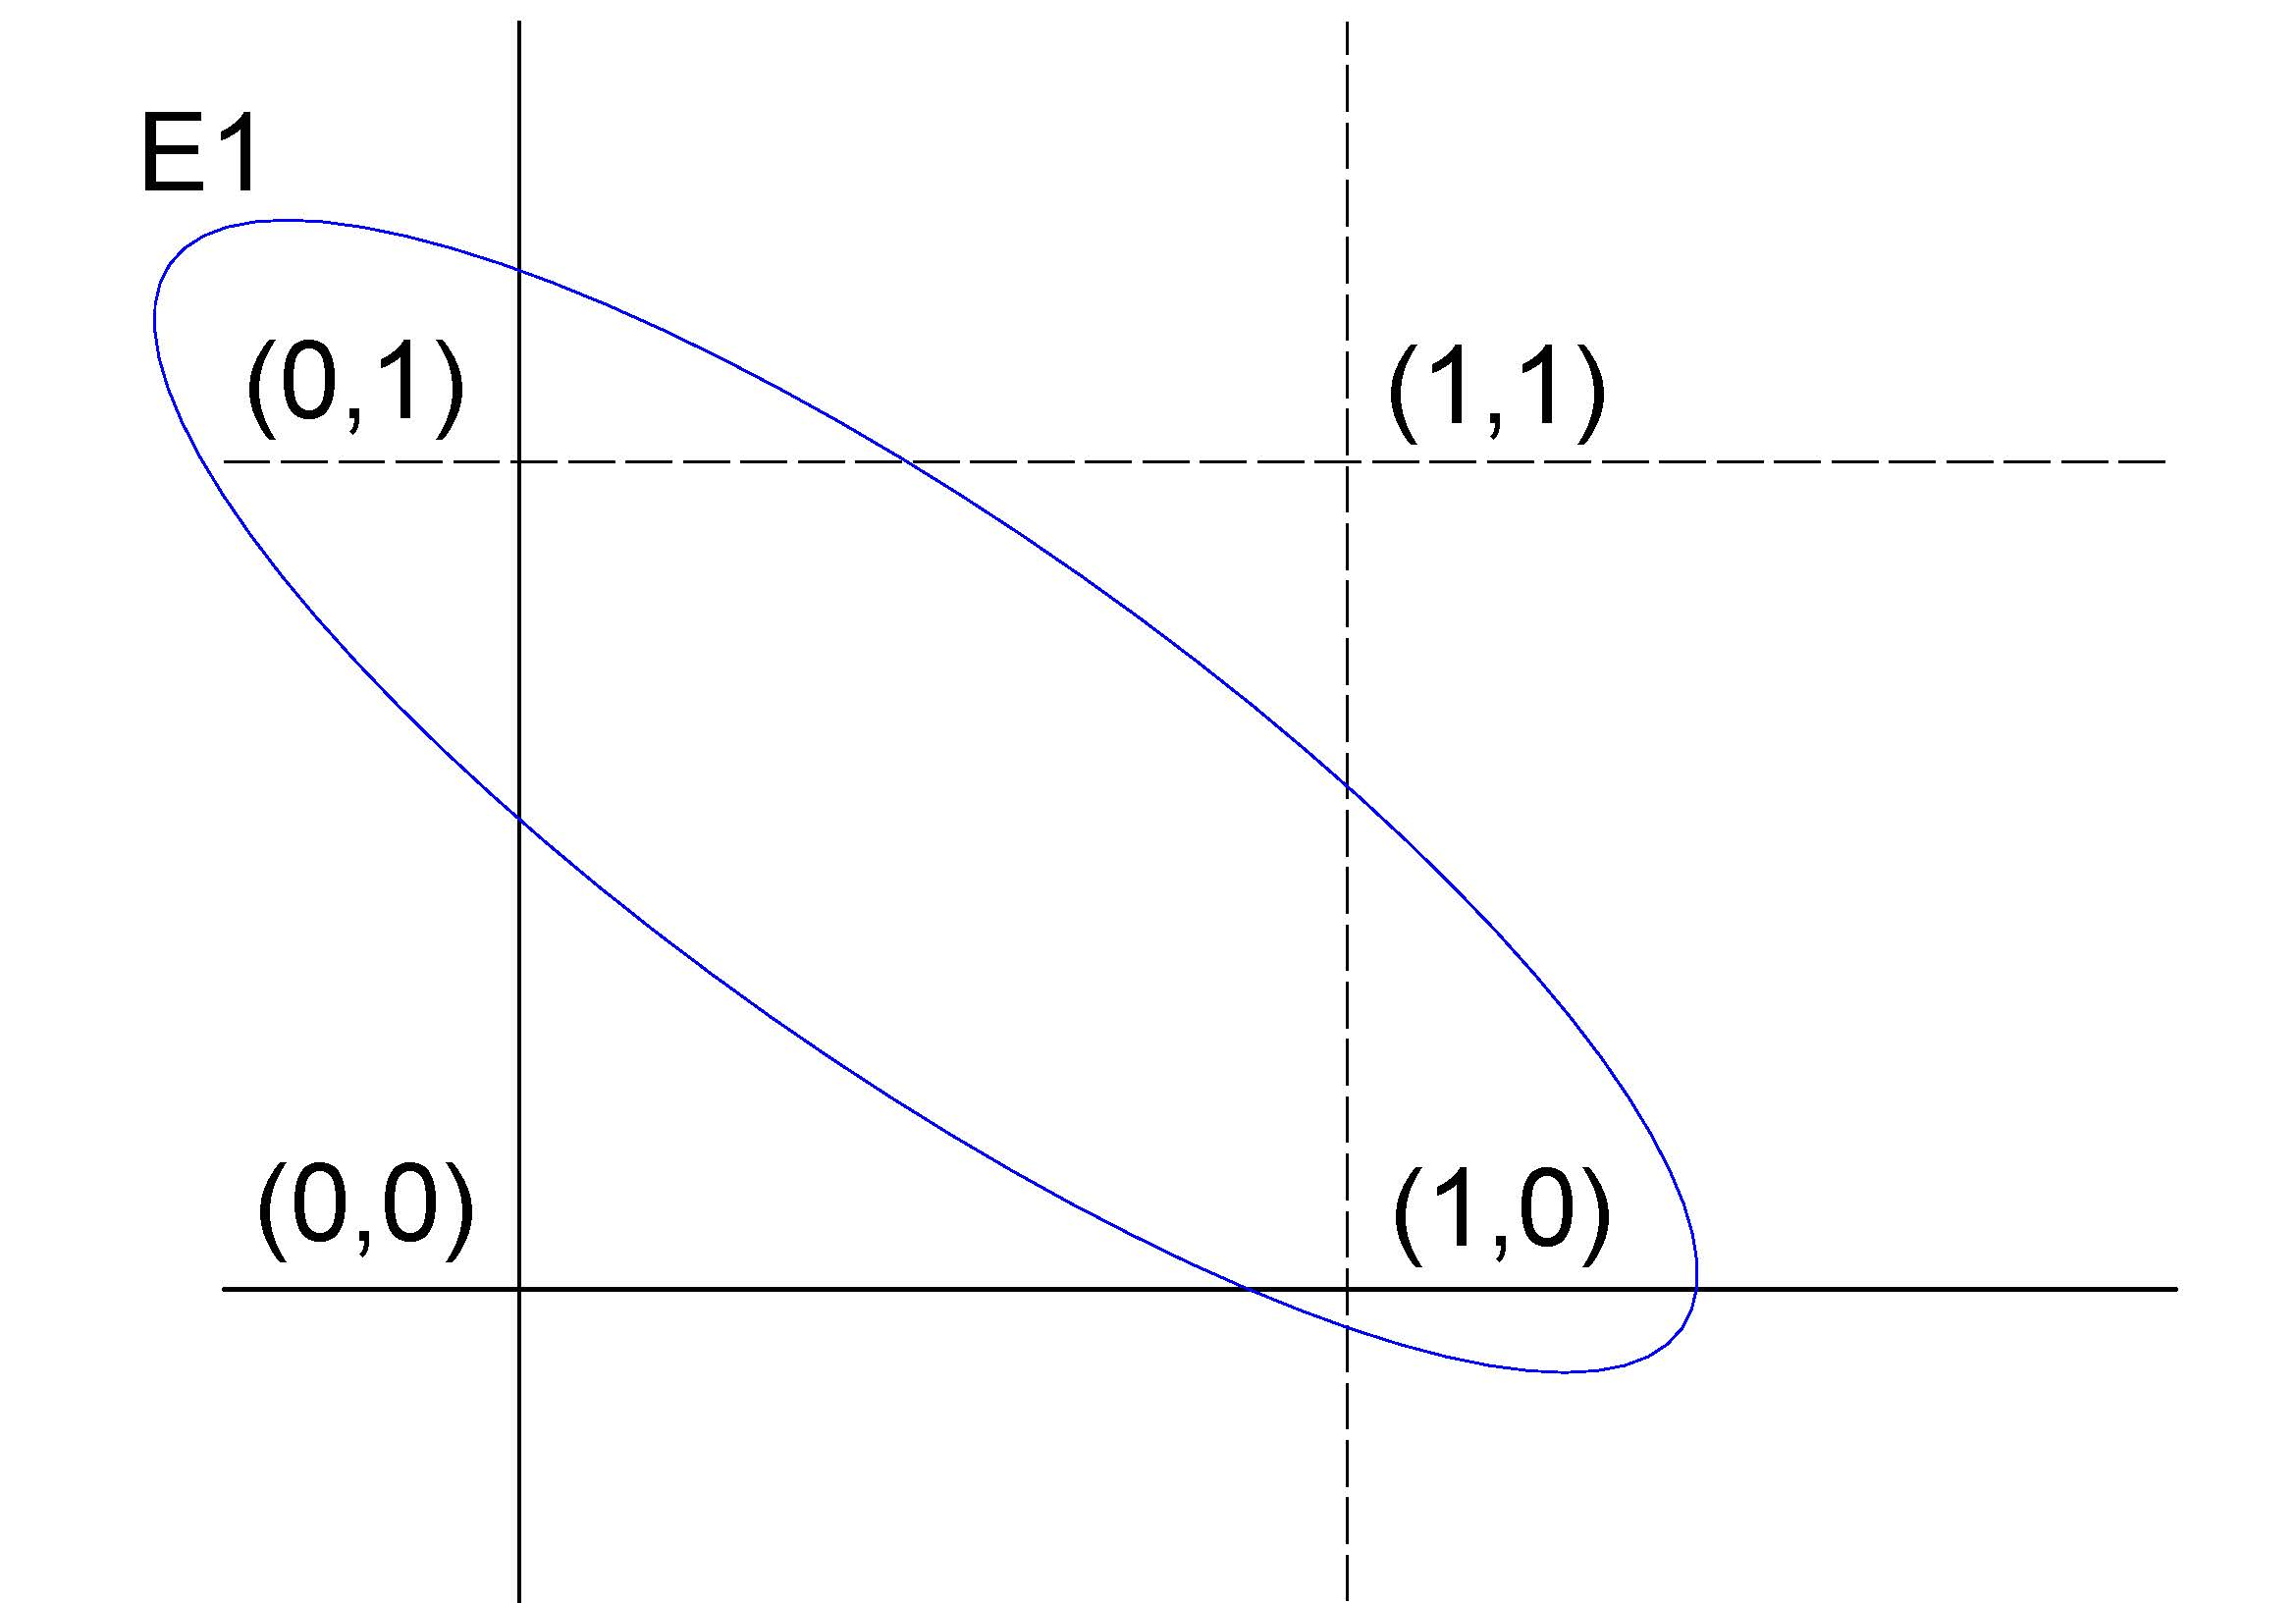
\includegraphics[width=0.5\linewidth]{images4/evento_grafico} 

}

\caption{Representação gráfico do espaço amostral do experimento aleatório e do evento de interesse definido}\label{fig:unnamed-chunk-61}
\end{figure}

Admita agora um outro experimento aleatório, estabelecido como a soma dos valores das faces de dois dados (ou um dado laçado duas vezes) aleatoriamente lançados. O espaço amostral desse experimento aleatório será um conjunto formado por 11 elementos.

\[
\Omega = \{\omega_{1}, \omega_{2}, \omega_{3}, \omega_{4}, \omega_{5}, \omega_{6}, \omega_{7}, \omega_{8}, \omega_{9}, \omega_{10}, \omega_{11}\}
\]

onde:

\begin{align*}
\omega_{1} & =  2\\
\omega_{2} & =  3\\
\omega_{3} & = 4\\
\omega_{4} & = 5\\
\omega_{5} & = 6\\
\omega_{6} & = 7 \\
\omega_{7} & = 8\\
\omega_{8} & = 9\\
\omega_{9} & = 10\\
\omega_{10} & = 11\\
\omega_{11} & = 12     
\end{align*}

Cada um dos elementos que compõem o espaço amostral, a soma dos valores numéricos das faces no lançamento de um dado por duas vezes, poderá resultar de diferentes combinações de valores. A Tabela \ref{tab:table1} abaixo apresenta todas as combinações possíveis de serem obtidas, bem como as proporções em relação ao total para cada elemento do espaço amostral.

\hfill\break

\begin{longtable}[]{@{}
  >{\raggedright\arraybackslash}p{(\columnwidth - 6\tabcolsep) * \real{0.2381}}
  >{\raggedright\arraybackslash}p{(\columnwidth - 6\tabcolsep) * \real{0.4206}}
  >{\raggedright\arraybackslash}p{(\columnwidth - 6\tabcolsep) * \real{0.1746}}
  >{\raggedright\arraybackslash}p{(\columnwidth - 6\tabcolsep) * \real{0.1667}}@{}}
\caption{\label{tab:table1} Quadro dos possíveis resultados de um experimento aleatório: somas dos valores numéricos das faces no lançamento de um dado por duas vezes}\tabularnewline
\toprule()
\begin{minipage}[b]{\linewidth}\raggedright
Soma
\end{minipage} & \begin{minipage}[b]{\linewidth}\raggedright
Possíveis combinações de resultados nos lançamentos
\end{minipage} & \begin{minipage}[b]{\linewidth}\raggedright
Frequência (\(n_{i}\))
\end{minipage} & \begin{minipage}[b]{\linewidth}\raggedright
Proporção (\(f_{i}\))
\end{minipage} \\
\midrule()
\endfirsthead
\toprule()
\begin{minipage}[b]{\linewidth}\raggedright
Soma
\end{minipage} & \begin{minipage}[b]{\linewidth}\raggedright
Possíveis combinações de resultados nos lançamentos
\end{minipage} & \begin{minipage}[b]{\linewidth}\raggedright
Frequência (\(n_{i}\))
\end{minipage} & \begin{minipage}[b]{\linewidth}\raggedright
Proporção (\(f_{i}\))
\end{minipage} \\
\midrule()
\endhead
& (primeiro,segundo) & & \\
2 & (1,1) & 1 & \(\frac{1}{36}\) \\
3 & (1,2); (2,1) & 2 & \(\frac{2}{36}\) \\
4 & (1,3); (2,2); (3,1) & 3 & \(\frac{3}{36}\) \\
5 & (1,4); (2,3); (3,2); (4,1) & 4 & \(\frac{4}{36}\) \\
6 & (1,5); (2,4); (3,3); (4,2); (5,1) & 5 & \(\frac{5}{36}\) \\
7 & (1,6); (2,5); (3,4); (4,3); (5,2); (6,1) & 6 & \(\frac{6}{36}\) \\
8 & (2,6); (3,5); (4,4); (5,3); (6,2) & 5 & \(\frac{5}{36}\) \\
9 & (3,6); (4,5); (5,4); (6,3) & 4 & \(\frac{4}{36}\) \\
10 & (4,6); (5,5); (6,4) & 3 & \(\frac{3}{36}\) \\
11 & (5,6); (6, 5) & 2 & \(\frac{2}{36}\) \\
12 & (6,6) & 1 & \(\frac{1}{36}\) \\
Totais & & 36 & \(\frac{1}{36}\) \\
\bottomrule()
\end{longtable}

\hfill\break

Se agora definimos nosso evento de interesse como sendo \textbf{``obter uma soma ímpar''}, nosso sucesso será verificado se ocorrer qualquer um desses elemetos do espaço amostral:

\[
F=\{3;5;7;9;11\}
\]
Nosso evento de interesse é um \emph{evento composto} pois é formado por 5 elementos do \emph{espaço amostral} \(\Omega\).

Um evento de interesse \(G\) sobre o espaço amostral \(\Omega\) tal que

\[
G=\Omega
\]

expressa que qualquer um dos elementos de \(\Omega\) atende ao evento \(G\) e assim, a chance de ocorrência do evento \(G\) será absoluta. Esse tipo de evento é chamado de \textbf{evento certo}.

Se definirmos em evento de interesse \(I\) com um resultado não pertencente aos possíveis resutados representados no \emph{espaço amostral} \(\Omega\), como, por exemplo, 13, ou então um conjunto vazio \(\varnothing\), esse evento será impossível de ocorrer. Esse tipo de evento é chamado de \textbf{evento impossível}.

Desse modo temos diferentes tipos de eventos de inetersse:

1- \emph{simples}: composto por apenas um elemento do espaço amostral;
2- \emph{composto}: composto por dois ou mais elementos do espaço amostral;
3- \emph{certo}: composto por todos os elementos do espaço amostral;\\
4- \emph{impossível}: composto por um elemento que não integra o espaço amostral.

\hypertarget{operauxe7uxf5es-com-conjuntos-diagramas-de-venn}{%
\subsection{Operações com conjuntos \& Diagramas de Venn}\label{operauxe7uxf5es-com-conjuntos-diagramas-de-venn}}

\hfill\break

Em muitos dos problemas de probabilidade, o evento de interesse pode residir em \textbf{combinações de dois ou elementos} do conjunto que representa o espaço amostral. Uniões, interseções e complementos são alguns termos que, doravante, serão muito utilizados.

\hfill\break

\begin{figure}

{\centering 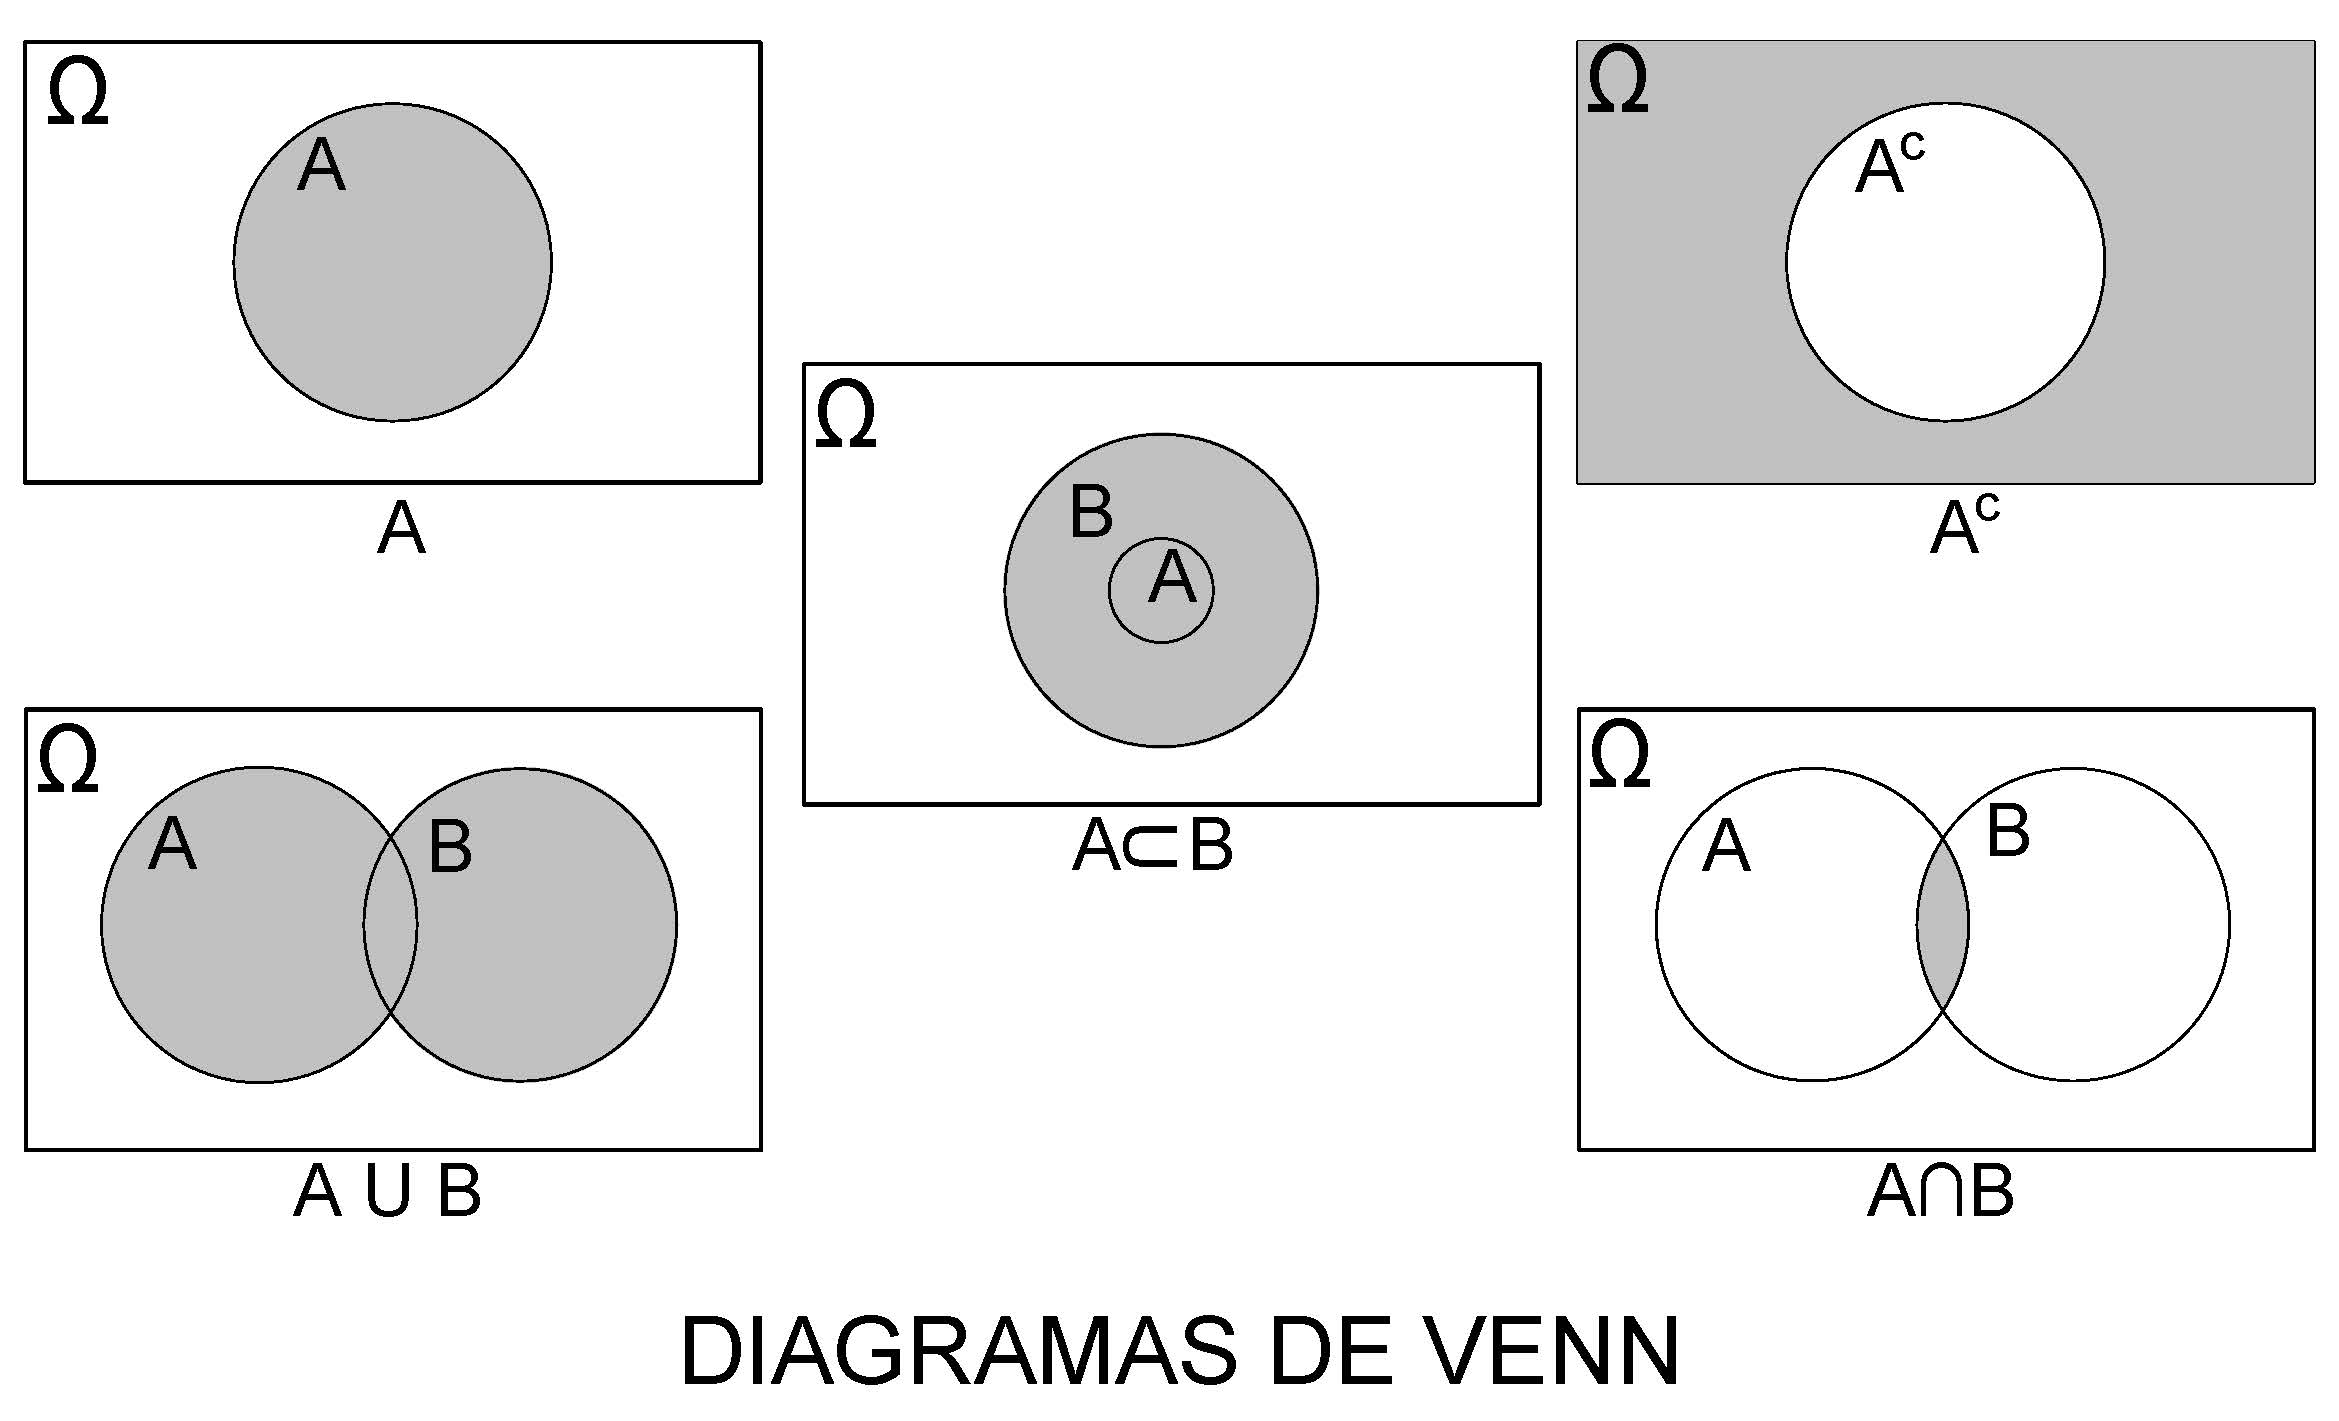
\includegraphics[width=0.8\linewidth]{images4/venn} 

}

\caption{Diagramas de Venn}\label{fig:unnamed-chunk-62}
\end{figure}

\hfill\break

\hypertarget{uniuxe3o-a-cup-b}{%
\subsubsection{\texorpdfstring{União \(A \cup B\)}{União A \textbackslash cup B}}\label{uniuxe3o-a-cup-b}}

Sejam \(A\) e \(B\) dois subconjuntos finitos de um espaço amostral \(Omega=\{1,2,3,4,5,6\}\) tais que \(A=\{1,2,3\}\) e \(B=\{2,4,6\}\).

Sua \emph{união}, representada por \(A \cup B\), é o subconjunto do espaço amostral \(\Omega\) que contém os elementos que pertençam \textbf{a \(A\), ou a \(B\) ou a ambos}. Desse modo, \(A \cup B =\{1,2,3,4,6\}\) e o Diagrama de Venn correspondente será:

\hfill\break

\begin{figure}

{\centering 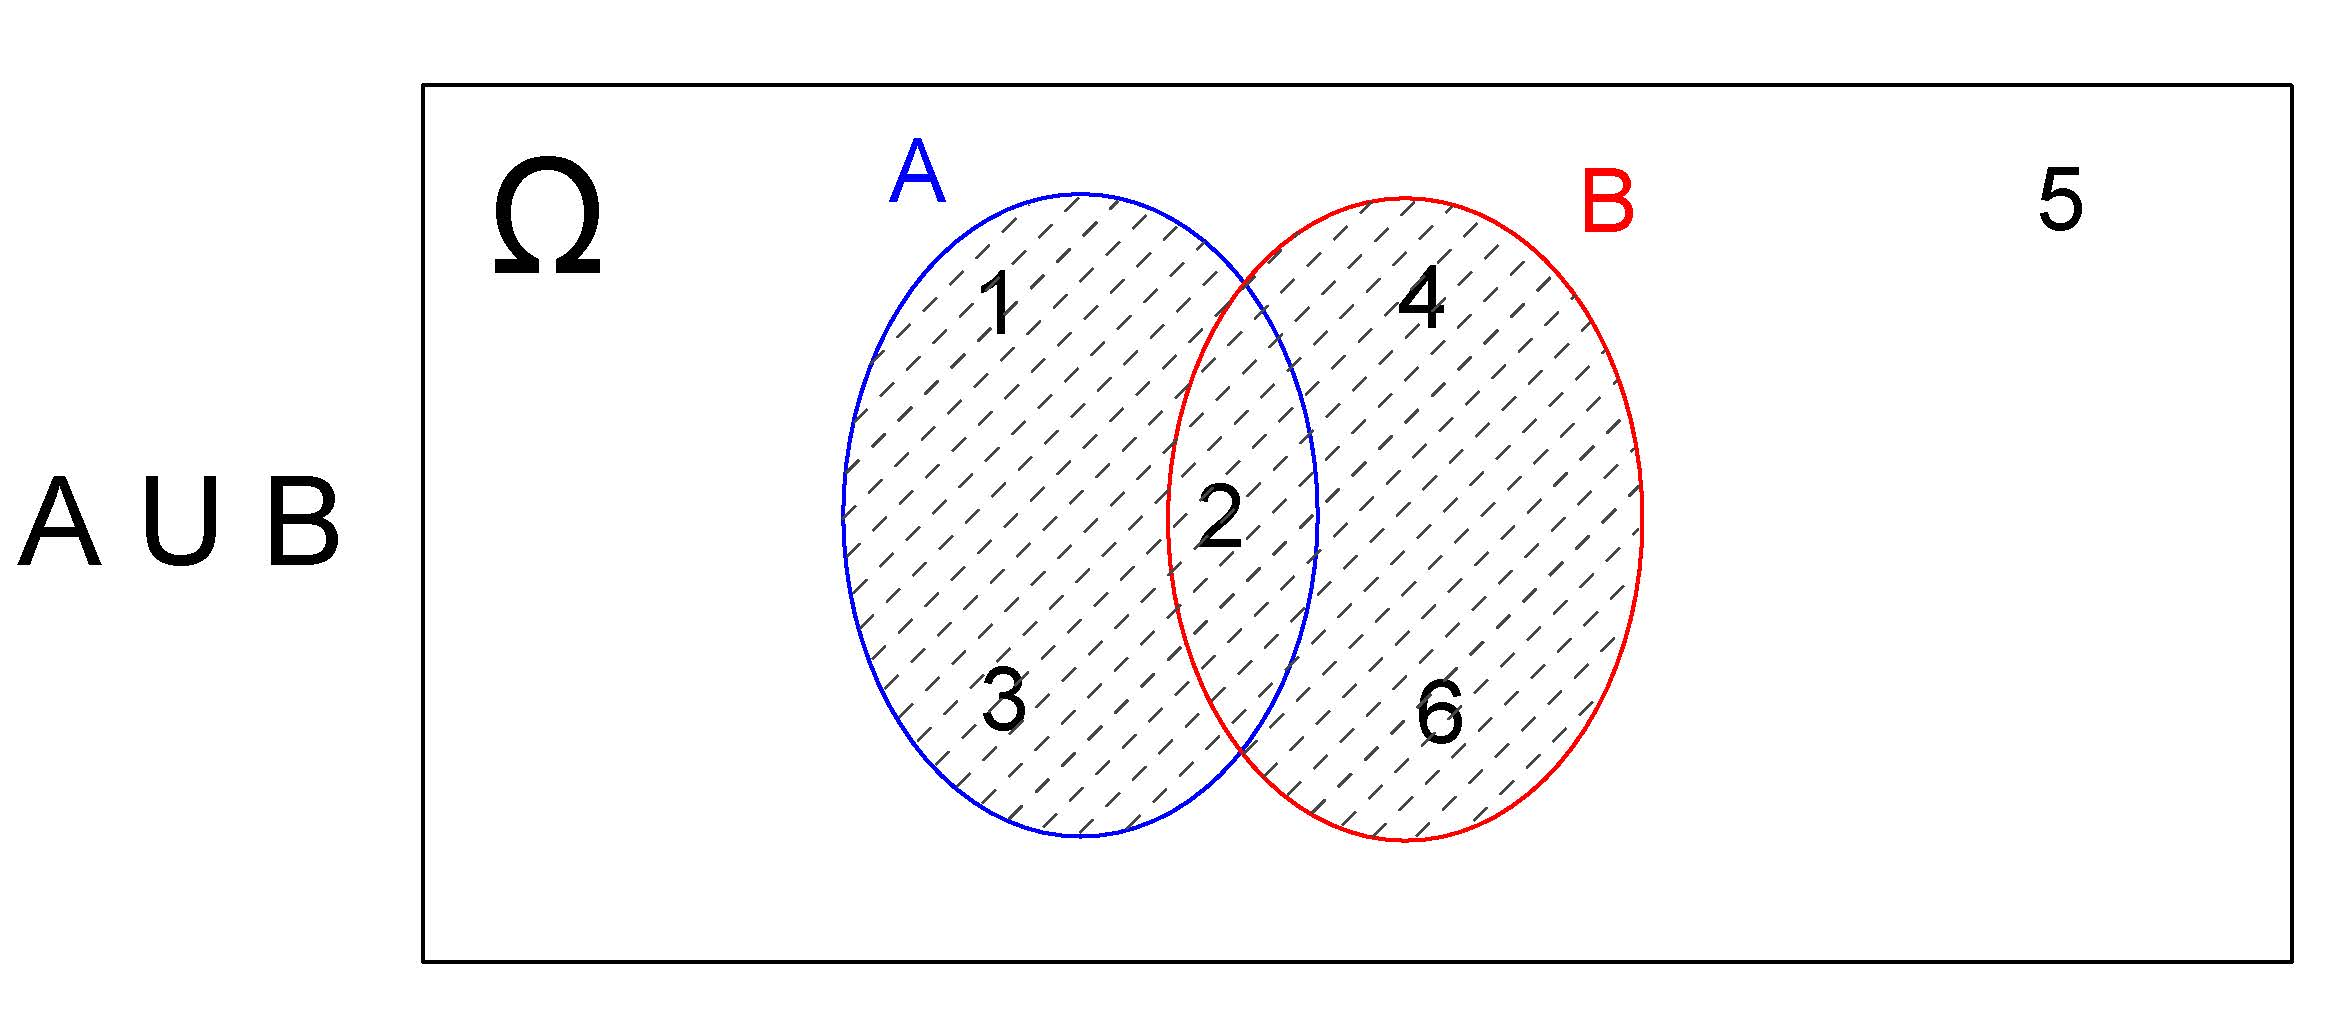
\includegraphics[width=0.8\linewidth]{images4/A_UN_B} 

}

\caption{União: $A \cup B$}\label{fig:unnamed-chunk-63}
\end{figure}

\hfill\break

\hypertarget{interseuxe7uxe3o-a-cap-b}{%
\subsubsection{\texorpdfstring{Interseção \(A \cap B\)}{Interseção A \textbackslash cap B}}\label{interseuxe7uxe3o-a-cap-b}}

Sua \emph{interseção}, representada por \(A \cap B\), é o subconjunto do espaço amostral \(\Omega\) que contém todos os elementos que pertencem \textbf{a ambos simultaneamente}. Desse modo, \(A \cap B =\{2\}\) e o Diagrama de Venn correspondente será:

\hfill\break

\begin{figure}

{\centering 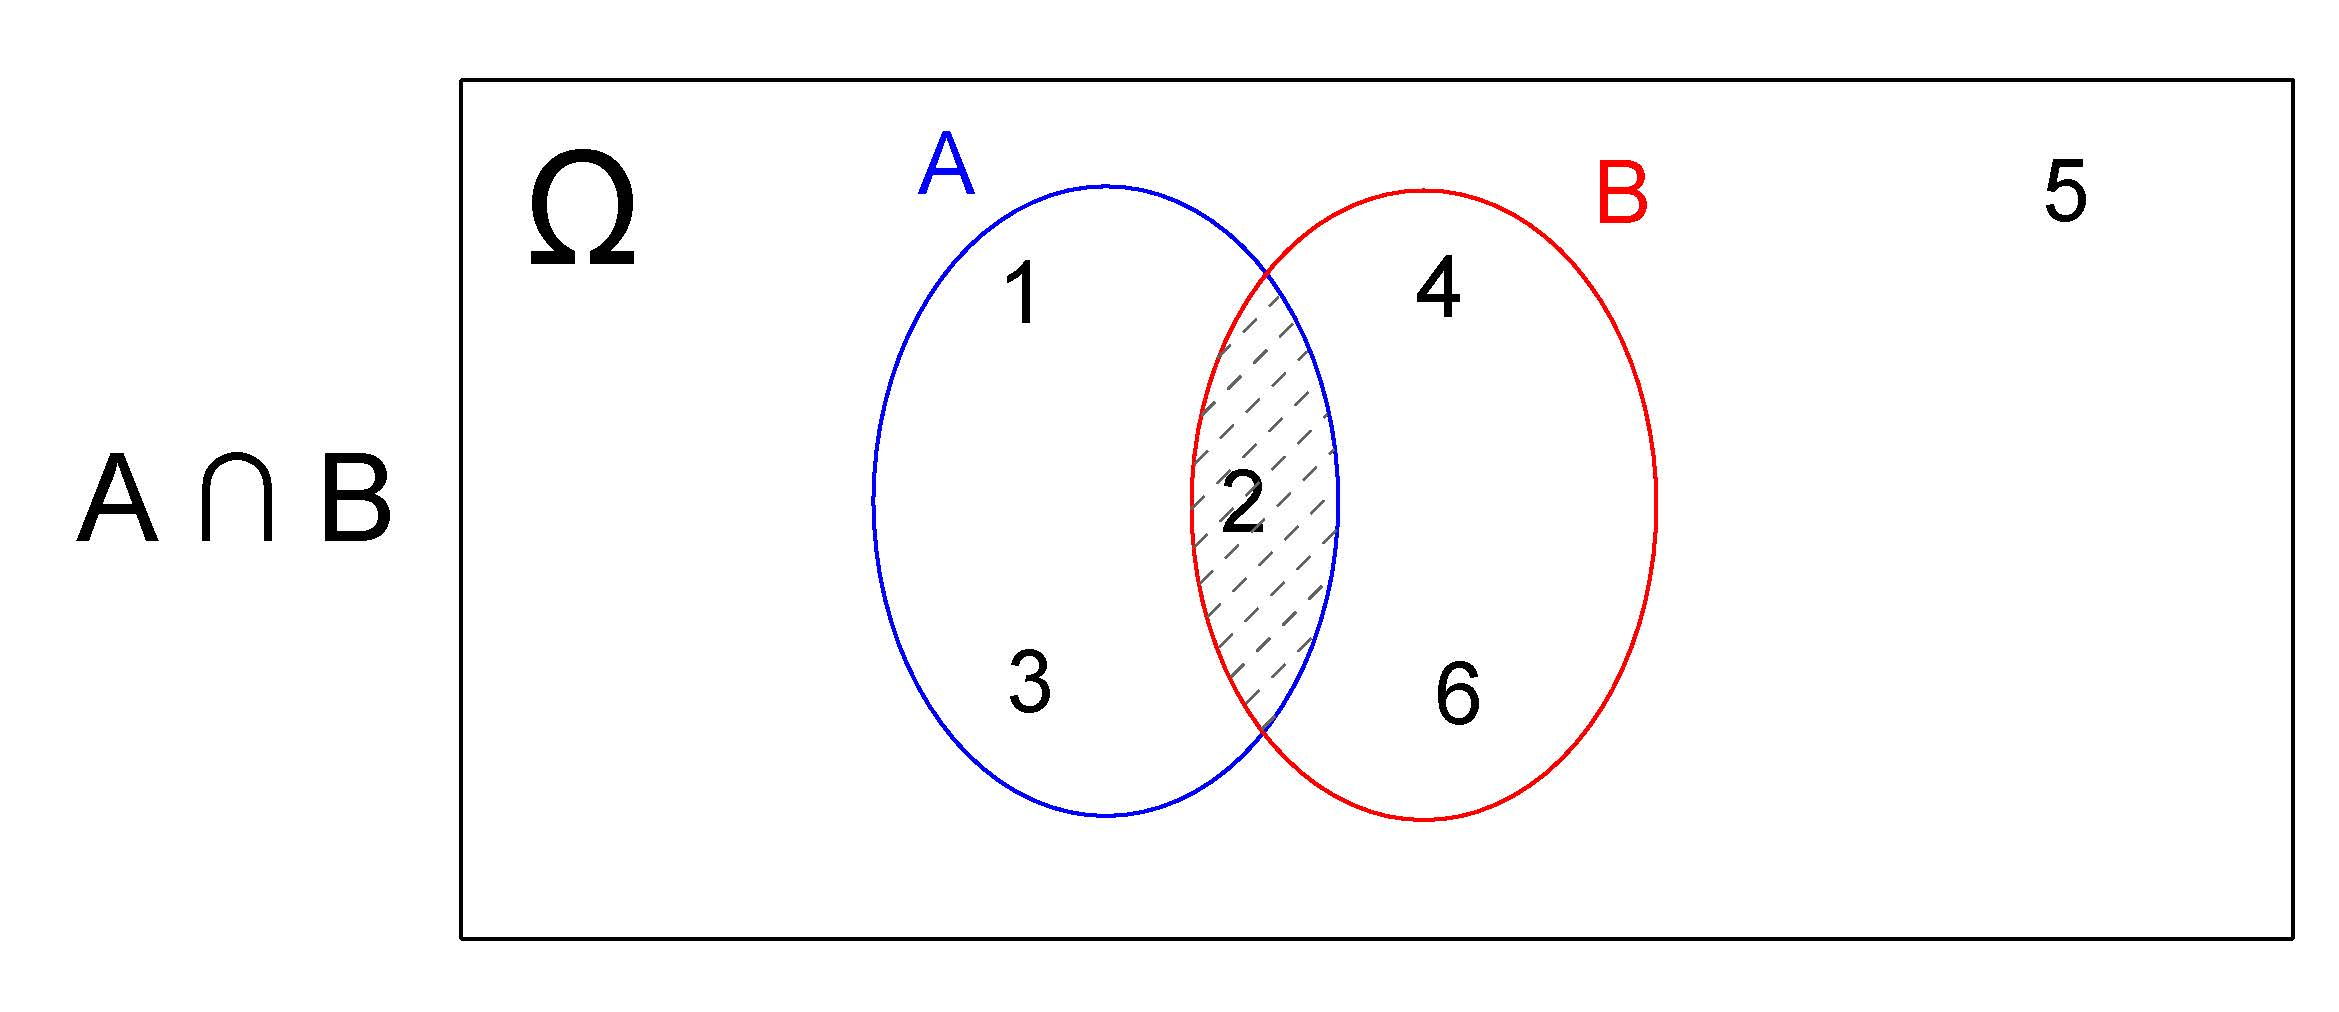
\includegraphics[width=0.8\linewidth]{images4/A_INTER_B} 

}

\caption{Interseção: $A \cap B$}\label{fig:unnamed-chunk-64}
\end{figure}

\hfill\break

Caso não exista nenhum elemento na interseção (ela é vazia) tem-se :

\[
A \cap B = \varnothing
\]

\hypertarget{complemmento-ac}{%
\subsubsection{\texorpdfstring{Complemmento \(A^{c}\)}{Complemmento A\^{}\{c\}}}\label{complemmento-ac}}

O \emph{complemento} de \(A\), representado por \(A^{c}\) (ou \(\stackrel{-}{A}\)), é o subconjunto do espaço amostral \(\Omega\) composto por todos os elementos que \textbf{não pertencem} a \(A\). Desse modo, \(\stackrel{-}{A} =\{4,5,6\}\) e o Diagrama de Venn correspondente será:

\hfill\break

\begin{figure}

{\centering \includegraphics[width=0.8\linewidth]{images4/COMP_A} 

}

\caption{Complementar  $A^{c}$}\label{fig:unnamed-chunk-65}
\end{figure}

\hfill\break

O \emph{complemento}\} de \(B\), representado por \(B^{c}\) (ou \(\stackrel{-}{B}\)), é o subconjunto do espaço amostral \(\Omega\) composto por todos os elementos que \textbf{não pertencem} a \(B\). Desse modo, \(\stackrel{-}{B} =\{1,3,5\}\) e o Diagrama de Venn correspondente será :

\hfill\break

\begin{figure}

{\centering \includegraphics[width=0.8\linewidth]{images4/COMP_B} 

}

\caption{Complementar de B}\label{fig:unnamed-chunk-66}
\end{figure}

\hypertarget{eventos-equiprovuxe1veis-e-nuxe3o-equiprovuxe1veis}{%
\subsection{Eventos equiprováveis e não equiprováveis}\label{eventos-equiprovuxe1veis-e-nuxe3o-equiprovuxe1veis}}

\hfill\break

Se todos os elementos que compõem um espaço amostral finito de um experimento aleatório possuem a mesma probabilidade de ocorrência é dito que esse espaço amostral é \textbf{uniforme} ou que seus elementos são \textbf{equiprováveis}.

No experimento de se lançar um dado e anotar o valor numérico de sua face todos os possíveis resultados apresentam a mesma probabilidade: \(\frac{1}{6}\).

Já no experimento de se lançar dois dados e se anotar a soma dos valores numéricos de suas faces as probabilidades são diferentes.

Um significativo resultado é que a soma das probabilidades associadas a cada um desses possíveis resultados é um (1) (antecipando um dos postulados do conceito axiomático de probabilidade).

\hypertarget{eventos-independentes}{%
\subsection{Eventos independentes}\label{eventos-independentes}}

\hfill\break

Quando a possibilidade de ocorrência de um evento de interesse (sucesso) em um determinado exeprimento aleatório não é afetada pelo resultado \textbf{prévio} de outro diz-se que esses dois eventos são \textbf{independentes}\}. Caso contrário são ditos dependentes ou condicionados. Mais adiante esse conceito será introduzido de um modo mais detalhado.

\hypertarget{eventos-mutuamente-exclusivos}{%
\subsection{Eventos mutuamente exclusivos}\label{eventos-mutuamente-exclusivos}}

Dois eventos que nunca poderão ocorrer simultaneamente são ditos mutuamente exclusivos. No experimento do lançamento da moeda por uma vez, nunca observaremos simultaneamente os eventos: \(E=\{(Cara)\}\) \textbf{e} \(F=\{(Coroa)\}\) e assim sua interseção é vazia:

\[
E \cap F = \varnothing 
\]

E por essa razão, se chamarmos de \(P(E)\) e \(P(F)\) as probabilidades de ocorrência desses reultados veremos que :

\[
P(E) \cap P(F) = 0
\]

\hypertarget{eventos-complementares}{%
\subsection{Eventos complementares}\label{eventos-complementares}}

Definido um evento de interesse qualquer pode-se observar apenas dois resultados: \textbf{ocorrer} ou \textbf{não} o sucesso; ou seja, um ou outro deverá forçosamente ocorrer.

Chama-se de evento complementar (\(E^{c}\) ou \(\stackrel{-}{E}\)) a um evento (\(E\)), aquele cuja probabilidade de sucesso seja:

\[
P(E^{c}) = 1 - P(E)
\]

Se a probabilidade de sucesso de que ele ocorra for \(P(E)=p\) e a de que ele não ocorra for \(P(E^{c}= q)\) vê-se que a soma dessas quantidades deverá ser \(p + q =1\) (novamente antecipando um dos postulados do conceito axiomático de probabilidade).

\hypertarget{probabilidade-1}{%
\section{Probabilidade}\label{probabilidade-1}}

\hypertarget{introduuxe7uxe3o-histuxf3rica}{%
\subsection{Introdução histórica}\label{introduuxe7uxe3o-histuxf3rica}}

De acordo com alguns historiadores, a Teoria das probabilidades teve início como um ramo da Matemática com as célebres cartas entre Blaise Pascal (1623-1662) e Pierre de Fermat (1607-1665), após uma consulta feita por um nobre cavaleiro (Antoine Gombaud, o \_Chevalier de Méré) a Pascal, relacionadas a como repartir um montante apostado em um jogo de dados caso ele tenha que ser interrompido antes de sua conclusão. Todavia o estudo não formal remonta a alguns séculos atrás.

\hfill\break

Probabilidade tem sido definida como sendo o estudo da frequência de aparição de um fenômeno em relação a todas as suas possíveis alternativas; ou seja, seu objeto é o estudo das possibilidades dos fenômenos aleatórios. O estudo das probabilidades possui, digamos assim, duas raízes históricas:

\hfill\break

1- a solução de problemas relacionados a jogos; e,\\
2- a análise estatística de dados atuariais.

\hfill\break

\begin{figure}

{\centering \includegraphics[width=0.8\linewidth]{images4/astralagus} 

}

\caption{Astralagus (um dos ossos que compõem o calcanhar, usado no Egito antigo como um dado rudimentar)}\label{fig:unnamed-chunk-67}
\end{figure}

\hypertarget{conceito-cluxe1ssico-ou-a-priori}{%
\subsection{\texorpdfstring{Conceito clássico ou \emph{a priori}}{Conceito clássico ou a priori}}\label{conceito-cluxe1ssico-ou-a-priori}}

Sob uma visão intuitiva, a probabilidade como uma medida da informação que temos sobre a possibilidade de ocorrência de um evento aleatório, pode ser definida como a medida numérica expressa em termos relativos (percentuais), obtida pela razão (proporção) entre o número de eventos favoráveis (sucessos) pelo número total de eventos prováveis no experimento (espaço amostral). Esse conceito de probabilidade é denominado \emph{clássico} ou \emph{a priori}:

A distribuição de frequências é um instrumento importante para a análise da variabilidade de experimentos aleatórios e, em particular, as frequências relativas são estimativas das probabilidades.

\[
P(E)= \frac{\text{número de resultados de interesse (sucessos)}}{\text{número total de resultados possíveis no espaço amostral}}
\]

Com o estabelecimento de suposições adequadas, um modelo teórico de probabilidade pode ser estabelecido sem a observação \emph{a priori} dos resultados de experimento aleatório, reproduzindo de modo razoável a distribuição das frequências quando o experimento é diretamente observado.

Consideremos o exemplo do experimento que consiste em se lançar um dado e observar o valor numérico de sua face. As suposições que deveriam ser estabelecidas \emph{a priori} são:

\begin{itemize}
\tightlist
\item
  só pode ocorrer uma das seis faces; e,
\item
  o dado utilizado não possui viés algum (não favorece face alguma).
\end{itemize}

Como todos os \(N\) resultados do espaço amostral apresentam uma \textbf{mesma probabilidade} de ocorrência, então a proporção teórica de ocorrência de qualquer um desse resultados poderá ser apresentado na forma vista na na forma vista na Tabela \ref{tab:table2}.

\[
P(E)= \frac{1}{N}
\]\\

\begin{longtable}[]{@{}
  >{\raggedright\arraybackslash}p{(\columnwidth - 14\tabcolsep) * \real{0.1418}}
  >{\raggedright\arraybackslash}p{(\columnwidth - 14\tabcolsep) * \real{0.1348}}
  >{\raggedright\arraybackslash}p{(\columnwidth - 14\tabcolsep) * \real{0.1348}}
  >{\raggedright\arraybackslash}p{(\columnwidth - 14\tabcolsep) * \real{0.1348}}
  >{\raggedright\arraybackslash}p{(\columnwidth - 14\tabcolsep) * \real{0.1348}}
  >{\raggedright\arraybackslash}p{(\columnwidth - 14\tabcolsep) * \real{0.1348}}
  >{\raggedright\arraybackslash}p{(\columnwidth - 14\tabcolsep) * \real{0.1348}}
  >{\raggedright\arraybackslash}p{(\columnwidth - 14\tabcolsep) * \real{0.0496}}@{}}
\caption{\label{tab:table2} Distribuição das proporções teóricas do um experimento aleatório: lançamento de um dado}\tabularnewline
\toprule()
\begin{minipage}[b]{\linewidth}\raggedright
Face
\end{minipage} & \begin{minipage}[b]{\linewidth}\raggedright
1
\end{minipage} & \begin{minipage}[b]{\linewidth}\raggedright
2
\end{minipage} & \begin{minipage}[b]{\linewidth}\raggedright
3
\end{minipage} & \begin{minipage}[b]{\linewidth}\raggedright
4
\end{minipage} & \begin{minipage}[b]{\linewidth}\raggedright
5
\end{minipage} & \begin{minipage}[b]{\linewidth}\raggedright
6
\end{minipage} & \begin{minipage}[b]{\linewidth}\raggedright
Total
\end{minipage} \\
\midrule()
\endfirsthead
\toprule()
\begin{minipage}[b]{\linewidth}\raggedright
Face
\end{minipage} & \begin{minipage}[b]{\linewidth}\raggedright
1
\end{minipage} & \begin{minipage}[b]{\linewidth}\raggedright
2
\end{minipage} & \begin{minipage}[b]{\linewidth}\raggedright
3
\end{minipage} & \begin{minipage}[b]{\linewidth}\raggedright
4
\end{minipage} & \begin{minipage}[b]{\linewidth}\raggedright
5
\end{minipage} & \begin{minipage}[b]{\linewidth}\raggedright
6
\end{minipage} & \begin{minipage}[b]{\linewidth}\raggedright
Total
\end{minipage} \\
\midrule()
\endhead
Proporção teórica & \(\frac{1}{6}\) & \(\frac{1}{6}\) & \(\frac{1}{6}\) & \(\frac{1}{6}\) & \(\frac{1}{6}\) & \(\frac{1}{6}\) & 1 \\
\bottomrule()
\end{longtable}

\hfill\break

Sendo equiprováveis todos os elementos do espaço amostral, todos terão a mesma probabilidade de ocorrência que será:

\begin{align*}
P(E) = & \frac{1}{N} \\
     = &  \frac{1}{6} \\
     = & \frac{1}{6}    
\end{align*}

Por essa razão sabe-se, \emph{a priori} a probabilidade de ocorrência de qualquer evento ao se realizar esse tipo de experimento aleatório uma única vez.

\hfill\break

\hypertarget{conceito-frequentista-ou-a-posteriori}{%
\subsection{\texorpdfstring{Conceito frequentista ou \emph{a posteriori}}{Conceito frequentista ou a posteriori}}\label{conceito-frequentista-ou-a-posteriori}}

\hfill\break

Todavia, se realizarmos o experimento aleatório anterior algumas vezes apenas, tal regularidade poderá não ser, naturalmente, observada: as frequências observadas (as quantidades obtidas para cada um dos valores numéricos das faces) apresentarão uma \textbf{grande irregularidade} diferindo das ferquência teóricas definidas.

Observa-se que os resultados das frequências observadas irá se estabilizar, aproximando-se das frequências teóricas, à medida que se repite esse experimento um número suficientemente grande de vezes.

Ao se repetir o experimento aleatório um grande número de vezes ( \(n\) tendendo a infinitas vezes), a quantidade de vezes que um determinado resultado foi verificado dividida por o número de repetições realizadas (\(n\)) irá se aproximar de sua proporção teórica.

É o que se denomina como \emph{regularidade estatística dos resultados} por essa propriedade não mais se necessita que os eventos sejam \emph{equiprováveis}.

\[
P\left(E\right)=\underset{n\to \infty }{lim}{\frac{F(E)}{n}}
\]

onde:

\begin{itemize}
\tightlist
\item
  \(P(E)\) é a probabilidade de ocorrência do evento \(E\);\textbackslash{}
\item
  \(F(E)\) é a frequência observada do evento \(E\); e,\textbackslash{}
\item
  \(n\) é o número de repetições do experimento.
\end{itemize}

Essa é a definição frequencial (\emph{a posteriori}):

1- refere-se à probabilidade empírica observada \emph{a posteriori};
2- tem por objetivo estabelecer um modelo adequado à interpretação de alguns tipos de experimentos aleatórios; e,
3- é a base para se formular um modelo teórico de distribuição de probabilidades como os que serão abordados mais adiante.

\hfill\break

\hypertarget{conceito-axiomuxe1tico}{%
\subsection{Conceito axiomático}\label{conceito-axiomuxe1tico}}

\hfill\break

Um \emph{axioma} é uma premissa considerada necessariamente evidente e verdadeira, fundamento de uma demonstração, porém ela mesma indemonstrável, originada, segundo a tradição racionalista, de princípios inatos da consciência ou, segundo os empiristas, de generalizações da observação empírica.

Admiti \(P\) uma função que opera sobre o espaço \(\Omega\); isto é, uma função que associa uma quantidade \(P(\Omega)\) a cada elemento \(\omega\) \(\in\) \(\Omega\).

\hfill\break

\begin{figure}

{\centering \includegraphics[width=0.8\linewidth]{images4/funcao_probabilidade} 

}

\caption{Representação gráfica da função $P(\Omega)$}\label{fig:unnamed-chunk-68}
\end{figure}

\hfill\break

Essa função \(P\) será uma \textbf{função de probabilidade} se, e somente se, satisfizer a \textbf{três axiomas} (postulados: conceitos iniciais necessários à construção ou aceitação de uma teoria) estabelecidos por Andrey Kolmogorov (1933).

\hfill\break

\begin{figure}

{\centering \includegraphics[width=0.4\linewidth]{images4/kolmogorov} 

}

\caption{Andrey Nikolaevich Kolmogorov  (1903-1987)}\label{fig:unnamed-chunk-69}
\end{figure}

\hfill\break

Kolmogoroff afirmou que uma \emph{Teoria das probabilidades} poderia ser desenvolvida a partir de \emph{axiomas}, da
mesma forma que a geometria e a álgebra, e a considerou como caso especial da \emph{Teoria da medida e integração} desenvolvida por Lebesgue, Borel e Fréchet. Ele estabeleceu como postulados as propriedades comuns das noções de probabilidade clássica e frequentista que, desta forma, viraram casos particulares da definição axiomática.

\hfill\break

\hypertarget{postulado-do-intervalo}{%
\subsubsection{Postulado do intervalo}\label{postulado-do-intervalo}}

A probabilidade de qualquer \(E\) \textbf{é um número real entre 0 e 1} (pode-se entender isso como uma convenção, onde entã se estabelece a medidad da probabilidade é um número positivo e que qualquer evento pode ter probabilidade de, no máximo, 1). Esse postulado está plenamente de acordo com a interpretação frequentista de probabilidade.

\[
0 \hspace{0.5cm} \leq P(\Omega) \hspace{0.5cm} \leq 1
\]\\

\hypertarget{postulado-da-certeza}{%
\subsubsection{Postulado da certeza}\label{postulado-da-certeza}}

O segundo postulado refere-se à probabilidade do \textbf{evento certo} ser igua a 1. No que diz respeito à interpretação frequentista, uma probabilidade de 1 implica que o evento em questão ocorrerá 100\% do tempo ou, em outras palavras, \textbf{que é certo que ele ocorra} (como, p.~exemplo, um experimento aleatório de se lançar dois dados e somar o valor de suas faces o evento certo poderia ser definido como observar uym valor menor que 13 ou maior que 2)

\[
P(\Omega) = 1
\]

\hfill\break

\hypertarget{postulado-da-aditividade-para-eventos-mutuamente-exclusivos}{%
\subsubsection{Postulado da aditividade para eventos mutuamente exclusivos}\label{postulado-da-aditividade-para-eventos-mutuamente-exclusivos}}

\hfill\break

\[
P\left(\bigcup _{n=1}^{\infty }{\omega}_{n}\right)=\sum _{n=1}^{\infty }P\left({\omega}_{n}\right)
\]

para qualquer sequência de eventos \textbf{mutuamente exclusivos} \(\{\omega_{1}, \omega_{2}, \omega_{3}, ..., \omega_{n}, ...\}\) (isto é, tal que \$\omega\emph{\{i\} \cap \omega}\{j\} \varnothing \$ se \(i \neq j\))

Tomando o terceiro postulado no caso mais simples, isto é, para \textbf{dois} eventos mutuamente exclusivos \(\omega_{1}\) e \(\omega_{2}\), pode ser facilmente visto que é satisfeito pela interpretação frequentista.

Se um evento ocorrer, digamos, 28\% das vezes, outro evento ocorrerá 39\%, \textbf{e os dois eventos não podem ocorrer ao mesmo tempo (ou seja, são mutuamente exclusivos)}, então um \textbf{ou outro} evento\} ocorrerão em 28 + 39 = 67\% das vezes. Assim, o terceiro postulado é satisfeito, e o mesmo tipo de argumento se aplica quando há mais de dois eventos mutuamente exclusivos.

\hfill\break

\textbf{Recapitulando}

\hfill\break

1- foi definido o conceito de \textbf{experimento aleatório} como sendo aquele cujos resultados não podem ser determinados com certeza antes de sua realização;\\
2- foi definido o conceito de \textbf{espaço amostral} de um experimento aleatório como sendo o conjunto de \textbf{todos os possíveis resultados} que ele pode apresentar;\\
3- foi definido que um \textbf{evento de interesse} é um subconjunto do espaço amostral no qual estamos particularmente interessados;\\
4- foi definida uma \textbf{função} que tem como domínio o espaço amostral e associa uma quantidade (entre \textbf{0} e \textbf{1}) a \textbf{cada elemento} do espaço amostral; e, por fim,\\
5- estabelecemos que \textbf{se} essa função atende a \textbf{três postulados} então ela será uma \textbf{medida da probabilidade} de ocorrẽncia de cada evento do espaço amostral em questão.

\hfill\break

Assim, quando uma função \(P\) associa uma quantidade \(P(\Omega)\) a um evento \(\omega\) e \(P(\Omega)\) atende aos três axiomas anteriormente estabelecidos, diz-se que que ela é a \textbf{função de probabilidade} de \(\Omega\).

\hfill\break

\hypertarget{regra-geral-da-adiuxe7uxe3o-de-probabilidades-de-eventos}{%
\subsection{Regra geral da adição de probabilidades de eventos}\label{regra-geral-da-adiuxe7uxe3o-de-probabilidades-de-eventos}}

\hfill\break

Considerem agora a Tabela \ref{tab:table3} de dupla entrada onde vemos a distribuição de alunos conforme seu sexo e o curso escolhido:

\hfill\break

\begin{longtable}[]{@{}
  >{\raggedright\arraybackslash}p{(\columnwidth - 6\tabcolsep) * \real{0.3425}}
  >{\raggedright\arraybackslash}p{(\columnwidth - 6\tabcolsep) * \real{0.3699}}
  >{\raggedright\arraybackslash}p{(\columnwidth - 6\tabcolsep) * \real{0.1918}}
  >{\raggedright\arraybackslash}p{(\columnwidth - 6\tabcolsep) * \real{0.0959}}@{}}
\caption{\label{tab:table3} Distribuição da quantidade de alunos segundo seu sexo e curso escolhido}\tabularnewline
\toprule()
\begin{minipage}[b]{\linewidth}\raggedright
Curso
\end{minipage} & \begin{minipage}[b]{\linewidth}\raggedright
Sexo
\end{minipage} & \begin{minipage}[b]{\linewidth}\raggedright
\end{minipage} & \begin{minipage}[b]{\linewidth}\raggedright
\end{minipage} \\
\midrule()
\endfirsthead
\toprule()
\begin{minipage}[b]{\linewidth}\raggedright
Curso
\end{minipage} & \begin{minipage}[b]{\linewidth}\raggedright
Sexo
\end{minipage} & \begin{minipage}[b]{\linewidth}\raggedright
\end{minipage} & \begin{minipage}[b]{\linewidth}\raggedright
\end{minipage} \\
\midrule()
\endhead
& Masculino (M) & Feminino (F) & Total \\
Matemática pura (M) & 70 & 40 & 110 \\
Matemática aplicada (A) & 15 & 15 & 30 \\
Estatística (E) & 10 & 20 & 30 \\
Computação (C) & 20 & 10 & 30 \\
Total & 115 & 85 & 200 \\
\bottomrule()
\end{longtable}

\hfill\break

Essa tabela nos possibilita calcular a probabilidade de ocorrência de diversos eventos de interesse que desejemos estabelecer.

\begin{quote}
Exemplo: seja o experimento aleatório de se escolher, aleatoriamente, um estudante qualquer desses quatro cursos. Assim, se definimos nosso evento de interesse \(M\) como sendo \textbf{M:sexo masculino}, a probabilidade de sucesso (que o indivíduo sorteado aleatoriamente seja do sexo masculino) será:
\end{quote}

\[
P(M) = \frac{115}{200}
\]

\begin{quote}
Exemplo: se nosso evento de interesse \(A\) como sendo \textbf{\(A:\) curso de matemática aplicada} , a probabilidade de sucesso (que o indivíduo sorteado aleatoriamente seja do curso de matemática aplicada será):
\end{quote}

\[
P(A) = \frac{30}{200}
\]

A partir dos eventos de interesse anteriormente estabelecidos, podemos definir outros eventos na forma de uniões (\(\cup\)) e interseções (\(\cap\)):

\begin{itemize}
\tightlist
\item
  uma união entre os dois eventos de interesse anteriores \(A\) e \(M\) é representada por \(A \cup M\) (alternativamente lê-se também \textbf{ou}) e representa um evento onde \textbf{pelo menos} um dos dois eventos básicos pode ocorrer: \textbf{ou} \(A\), \textbf{ou} \(M\) \textbf{ou ambos}; e,\\
\item
  uma interseção dos dois eventos de interesse anteriores \(A\) e \(M\) é representada por \(A \cap M\) (alternativamente lê-se também \textbf{e}) e representa um evento onde \textbf{os dois eventos} básicos devem ocorrer: \(A\) \textbf{e} \(M\).
\end{itemize}

\begin{quote}
Exemplo: se definimos nosso evento de interesse (\(P(A \cap M)\)) como sendo \textbf{sexo masculino e cursando matemática aplicada}. Facilmente podemos visualizar na Tabela \ref{tab:table3} que apenas 15 alunos do curso do evento de interesse (matemática aplicada) são do sexo do segundo evento de interesse (masculino), em relação a todo espaço amostral e assim:
\end{quote}

\[
P(A \cap M) = \frac{15}{200}
\].

\begin{quote}
Exemplo: consideremos agora o evento de interesse (\(P(A \cup M)\)) como sendo \textbf{sexo masculino ou cursando matemática aplicada}.
\end{quote}

Na Tabela \ref{tab:table3} temos as duas probabilidades \textbf{marginais}:

\begin{enumerate}
\def\labelenumi{\arabic{enumi}.}
\tightlist
\item
  \(P(A)=\frac{30}{200}\) (curso: matemática aplicada); e,
  2- \(P(M)=\frac{115}{200}\) (sexo masc).
\end{enumerate}

Poderíamos intuir equivocadamente que:

\[
P(A \cup M) = P(A) + P(M) = \frac{30}{200} + \frac{115}{200} = \frac{145}{200}
\]

Tal raciocínio é errado pois iria considerar por \textbf{duas vezes} os alunos do \textbf{sexo masculino}. Uma fração da quantidade global (115) de alunos do \textbf{sexo masculino} já considera aqueles que estão matriculados no curso de \textbf{matemática aplicada} (15). É preciso \textbf{subtrair} da soma das probabilidades marginais essa \textbf{parcela em comum} que é a interseção dos dois eventos básicos.

A resposta correta será:

\[
P(A \cup M) = P(A) + P(M) - P(A \cap M) = \frac{30}{200} + \frac{115}{200} -\frac{15}{200} = \frac{130}{200}
\].

\hfill\break

Portanto, para quaisquer eventos de intersse \(A\) e \(B\), podemos estabelecer uma \textbf{regra geral para a adição de probabilidades de dois eventos quaiquer} como:

\[
P(A \cup B) = P(A) + P(B) - P(A \cap B)
\]

Se \(A\) e \(B\) forem \textbf{mutuamente exclusivos}, a interseção entre eles será vazia (\(A \cap B =\varnothing\)) e, assim, essa probabiidade é zero. Nessa situação, a probabilidade de \(P(A \cup B)\) fica reduzida a uma \textbf{regra particular para a adição de probabilidades de eventos mutuamente exclusivos}:

\[
P(A \cup B) = P(A) + P(B)
\]

\begin{quote}
Exemplo: Seja o experimento aleatório de se lançar um dado (com seis faces) e observar o valor numérico da face que ficar exposta. Qual a probabilidade de se observar os valores \(1\) \textbf{ou} \(4\)?
\end{quote}

Definindo os eventos de interesse:

1- \(E_{1}=\text{sair face 1}\) (\(P(E_{1})=\frac{1}{6}\)); e,\\
2- \(E_{4}=\text{sair face 4}\) (\(P(E_{4})=\frac{1}{6}\)).

Pede-se \(P(E_{1} \cup E_{4})\).

Como \(E_{1}\) e \(E_{4}\) são *eventos mutuamente exclusivos**: \(E_{1} \cap E_{4}=\varnothing\) (portanto a probabilidade é zero), então \(P(E_{1} \cup E_{4}) = P(E_{1}) + P(E_{4}) = \frac{1}{6} + \frac{1}{6}= \frac{1}{3}\).

\begin{quote}
Exemplo: Uma população é composta por 20 pessoas que consomem o produto \textbf{A}, 30 pessoas que consomem o produto \textbf{B} e 50 pessoas que consomem o produto \textbf{C} . Um pesquisador de mercado seleciona aleatoriamente uma pessoa desta população. \textbf{Sabendo que uma pessoa não consome mais de um produto ao mesmo tempo}, qual a probabilidade de ter sido selecionada uma pessoa que consome os produtos \textbf{A ou C}?
\end{quote}

Solução:

Definindo os eventos de interesse e as probabilidades associadas:

1- \(E_{A}=\text{consumidor do produto A}\): \(P(E_{A}=\frac{20}{100}\));\\
2- \(E_{B}=\text{consumidor do produto B}\): \(P(E_{B}=\frac{30}{100}\)); e,\\
3- \(E_{C}=\text{consumidor do produto C}\): \(P(E_{C}=\frac{50}{100}\)).

Pela regra geral da adição de probabilidades de dois eventos quaiquer sabemos que:

\[
P(E_{A} \cup E_{C}) = P(E_{A}) + P(E_{C}) - P(E_{A} \cap E_{C})
\]

Como foi estabelecido no enunciado que uma pessoa \textbf{não} consome mais de um produto ao mesmo tempo (esses eventos são, portanto, \textbf{mutuamente exclusivos}: \(E_{A} \cap E_{C}=\varnothing\)) a probabilidade pedida será:

\begin{align*}
P(E_{A} \cup E_{C}) & = P(E_{A}) + P(E_{C}) - P(E_{A} \cap E_{C}) \\
                    & = \frac{20}{10} + \frac{50}{100} - 0 \\
                    & =  \frac{70}{100} \\
                    & =  0,70    
\end{align*}

\hypertarget{probabilidade-de-eventos-condicionados}{%
\subsection{Probabilidade de eventos condicionados}\label{probabilidade-de-eventos-condicionados}}

\hfill\break

Dois eventos \(A\) e \(B\) de um experimento aleatório qualquer são ditos \textbf{condicionados} quando a ocorrência prévia de um deles impõe \textbf{uma restrição} no espaço amostral do segundo.

A \textbf{probabilidade} de um evento qualquer \(A\) \textbf{condicionada} a um segundo evento \(B\) é representada como \(P(A|B)\). A \emph{barra} verical pode ser ``lida'' adotando-se termos correlatos que facilitam o entendimento da relação existente, tais como :

\begin{itemize}
\tightlist
\item
  probabilidade de \(A\) \textbf{posto que} ocorreo \(B\);
\item
  probabilidade de \(A\) \textbf{admitindo-se} que ocorreu \(B\);
\item
  probabilidade de \(A\) \textbf{considerando-se} que ocorreu \(B\),
\end{itemize}

e seu cálculo é feito pela \textbf{regra geral da probabilidade de dois eventos condicionados}:

\begin{align*}
P(A|B) & = \frac{ P(A\cap B)}{ P(B)} \\
P(B|A) & = \frac{ P(B\cap A)}{ P(A)}
\end{align*}

sendo \(P(B)>0\) e \(P(A)>0\) nas expressões acima.

De modo geral, admita que os eventos \(E_{1}\), \(E_{2}\),\ldots,\(E_{n}\) formam uma partição do espaço amostral.

Os eventos não têm interseções entre si e a união destes é igual ao espaço amostral e seja \(A\) um evento qualquer desse espaço.

Então a probabilidade de ocorrência desse evento será dada por:

\begin{align*}
P(A) & = P(A \cap E_{1}) +  P(A \cap E_{2}) + \dots + P(A \cap E_{n}) \\
     & = P(E_{1}) \times P(A|E_{1}) + P(E_{2}) \times P(A|E_{2}) + \dots + \\
     & P(E_{n}) \times P(A|E_{n})\\
\end{align*}

\hfill\break

\begin{quote}
Exemplo: Consideremos a Tabela \ref{tab:table3} que apresenta o cruzamento do sexo dos alunos pelos seus respectivos cursos. Vamos definir os eventos \textbf{\(Fem:\) sexo feminino} e \textbf{\(Est:\) cursar estatística}. Como calcular a probabilidade condicionada de nosso evento de interesse \textbf{\(P(Fem|Est)\)} (a probabilidade de um aluno aleatoriamente escolhido ser do sexo \textbf{feminino}, \textbf{dado} que ele cursa \textbf{estatística})?
\end{quote}

\begin{align*}
P(Fem|Est) & = \frac{ P(Fem \cap Est)}{ P(Est)} \\
           & = \frac{20}{30} = \frac{2}{3}    
\end{align*}

Esse cálculo é facilmente entendido observando-se as celulas da distribuição de frequências na Tabela \ref{tab:table3}.

\begin{quote}
Exemplo: Considerem a Tabela \ref{tab:table4} que relaciona a ida à praia de uma certa pessoa às condições climáticas do dia.
\end{quote}

\begin{longtable}[]{@{}lllllllllll@{}}
\caption{\label{tab:table4} Condicionamento de passeios à praia em relação às condições climáticas observadas}\tabularnewline
\toprule()
Dia & 1 & 2 & 3 & 4 & 5 & 6 & 7 & 8 & 9 & 10 \\
\midrule()
\endfirsthead
\toprule()
Dia & 1 & 2 & 3 & 4 & 5 & 6 & 7 & 8 & 9 & 10 \\
\midrule()
\endhead
Foi à praia? & N & S & N & S & S & S & N & N & S & S \\
Fez sol? & N & S & N & S & N & S & S & N & S & S \\
\bottomrule()
\end{longtable}

Baseado nos dados coletados responda:

1- Qual a probabilidade dessa pessoa ir à praia?\\
2- Sabendo-se que fez Sol, qual a probabilidade dessa pessoa ir à praia?\\
3- Os eventos \textbf{ir à praia} e \textbf{fazer Sol} são independentes ou condicionados?

Da Tabela \ref{tab:table4} extraímos as seguintes probabilidades:

\begin{align*}
P(IP) & = \frac{6}{10}= 0,60 \\
P(FS) & = \frac{6}{10}= 0,60 \\
P(IP \cap FS) & = \frac{5}{10} \\
    & = 0,50 
\end{align*}

A partir delas podemos calcular a seguinte probabilidade condicionada:

\begin{align*}
P(IP|FS) & = \frac{ P(IP \cap F)}{ P(FS)} \\
       & = \frac{5}{6} \\
       & = 0,83     
\end{align*}

A probabilidade dessa pessoa ir à praia (\(P(IP)\)) é 0,60; \textbf{mas} quando faz Sol a probabilidade (\(P(IP|FS)\)) dela aumenta para 0,83.

Assim, os eventos \(IP\) e \(FS\) são condicionados: essa pessoa vai à praia 60\% dos dias analisados; mas, \textbf{quando faz sol}, ela vai em 83\% dos dias (a presença de Sol altera a probabilidade dela ir à praia).

\begin{quote}
Exemplo: Em uma cidade existem 15.000 usuários de telefonia, dos quais 10.000 possuem telefones fixos, 8.000 telefones móveis e 3.000 telefones fixos e móveis. Seja o experimento aleatório de uma operadora de telefone móvel selecionar uma pessoa dessa cidade para oferecer uma promoção do tipo ``Fale Grátis de seu Móvel para seu Fixo''.
\end{quote}

Responda:

1- Sorteando-se aleatoriamente um cliente dessa operadora, se soubermos antecipadamente que ele tem telefone móvel, qual a probabilidade de esse cliente tenha telefone fixo também?\\
2- Sabendo-se que ele tem telefone fixo, qual a probabilidade de ele tenha telefone móvel também?

O espaço amostral de todos esses possíveis eventos pode ser ilustrado pelo diagrama de Venn abaixo:

\hfill\break

\begin{figure}

{\centering \includegraphics[width=0.5\linewidth]{images4/exercicio} 

}

\caption{Diagrama de Venn do espaço amostral}\label{fig:venn}
\end{figure}

\hfill\break

Do diagrama apresentado na Figura\ref{fig:venn} podemos extrair imediatamente as probabilidades pedidas:

\begin{itemize}
\tightlist
\item
  \(P(F|M)\) (probabilidade de ter uma linha fixa sabendo que possui um telefone móvel); e,
\item
  \(P(M|F)\) (probabilidade de ter uma linha móvel sabendo que possui um telefone fixo):
\end{itemize}

\hfill\break

\begin{align*}
P(F|M) & = \frac{n(MF)}{n(M)}\\
       & =\frac{3000}{8000}\\
       & = 0,375 
\end{align*}\\

e

\hfill\break

\begin{align*}
P(M|F) & = \frac{n(MF)}{n(F)} \\
       & =\frac{3000}{10000} \\
       & = 0,300 
\end{align*}

\hfill\break

Mas também podemos calcular as probablidades do modo como explicado no começo desta sessão. Definindo-se os eventos \textbf{\(F:\) telefone fixo} e \textbf{\(M:\) telefone móvel}, a primeira pergunta pede \(P(F|M)\):probabilidade de ter um telefone fixo sabendo que ele tem um telefone móvel:

\hfill\break

\begin{align*}
P(F|M) & =  \frac{P(F \cap M)}{P(M)} \\
       & = \frac{ \frac{3000}{15000} }{\frac{8000}{15000} }\\
       & = 0,375.
\end{align*}\\

A segunda pede \(P(M|F)\): probabilidade de ter um telefone móvel sabendo que ele tem um telefone fixo:

\hfill\break

\begin{align*}
P(M|F) & = \frac{P(M \cap F)}{P(F)} \\
       & = \frac{ \frac{3000}{15000} }{\frac{10000}{15000} } \\
       & = 0,300
\end{align*}

\hfill\break

\begin{quote}
Exemplo: Considere a Tabela \ref{tab:table5} onde são expostos os resultados de uma pesquisa relacionada ao gosto pela prática de tênis entre alunos e alunas. Definindo-se os eventos \textbf{\(A\):``gostar de tênis''} e \textbf{\(B\):``ser do sexo feminino''}, calcule as probabilidade pedidas ao se sortear, aleatoriamente, uma das pessoas pesquisadas.
\end{quote}

\hfill\break

1- Qual a probabilidade de que goste de tênis (\(P(T)\))?\\
2- Qual probabilidade de que não goste de tênis (\(P(T^{c})\))?\\
3- Qual a probabilidade de que seja do sexo feminino \textbf{ou} goste de tênis: (\(P(F \cup T)\))?\\
4- Sabendo-se que foi sorteada uma aluna, qual a probabilidade de que goste de tênis (\(P(T|F))\)?\\
5- Verifique se os eventos \textbf{\(T\): ``gostar de tênis''} e \textbf{\(F\):``ser do sexo feminino''} são condicionados ou independentes (\(P(T \cap F) \stackrel{?}{=} P(T) \times P(F)\)))

\hfill\break

\begin{longtable}[]{@{}llll@{}}
\caption{\label{tab:table5} Distribuição da quantidade de alunos segundo seu sexo e a preferência por tênis}\tabularnewline
\toprule()
& Sexo & & \\
\midrule()
\endfirsthead
\toprule()
& Sexo & & \\
\midrule()
\endhead
Curso & & & \\
& Masculino (M) & Feminino (F) & Total \\
Gostam de tênis (T) & 400 & 200 & 600 \\
Não gostam de tênis (NT) & 50 & 50 & 100 \\
Total & 450 & 250 & 700 \\
\bottomrule()
\end{longtable}

\hypertarget{dependuxeancia-independuxeancia-de-eventos}{%
\subsection{Dependência \& independência de eventos}\label{dependuxeancia-independuxeancia-de-eventos}}

Pela \textbf{regra geral da probabilidade de dois eventos eventos condicionados}:

\begin{align*}
P(A|B) & = \frac{ P(A\cap B)}{ P(B)} \\
P(B|A) & = \frac{ P(B\cap A)}{ P(A)}
\end{align*}

Como a probabilidade de interseção não se altera (\(P(A\cap B)=P(B\cap A)\)), podemos reescrever essas duas expressões:

\begin{align*}
P(A \cap B) & =   P(A|B) \times P(B)  \\
P(A\cap B)  & =   P(B|A) \times P(A)    
\end{align*}

com \(P(B)>0\) e \(P(A)>0\) nas expressões acima.

Se os eventos \(A\) e \(B\) são guardam nenhuma relação de condicionamento eles são chamadas de \textbf{eventos independentes}. Equivale dizer que \(P(A|B)=P(A)\) (ou \(P(B|A)=P(B)\)), a probabilidade de \(A\) não se altera pela prévia ocorrência de \(B\) (ou a de \(B\) pelo de \(A\)).

Portanto, \textbf{dois eventos são denominados independentes se, e somente se}:

\[
P (A \cap B)= P(A) \times P(B)
\]

\begin{quote}
\textbf{Independência e correlação}: se duas variáveis aleatórias são \textbf{independentes} não há associação de natureza alguma entre elas, \textbf{inclusive a linear}, um caso particular de correlação. Todavia uma \textbf{correlação linear nula} não implica em \textbf{independência} posto existirem várias outras formas outras de relacionamento (quadrática, cúbica, \dots).
\end{quote}

\hfill\break

\begin{figure}

{\centering \includegraphics[width=0.5\linewidth]{images4/indepn_correlacao} 

}

\caption{Independência implica em ausência de qualquer tipo de associação (a recíproca não se aplica}\label{fig:unnamed-chunk-70}
\end{figure}

\hfill\break

\hypertarget{regra-geral-do-produto-das-probabilidades-para-eventos-independentes}{%
\subsection{Regra geral do produto das probabilidades para eventos independentes}\label{regra-geral-do-produto-das-probabilidades-para-eventos-independentes}}

Se \(E_{1}\), \(E_{2}\), \ldots, \(E_{n}\) são eventos totalmente independentes \textbf{entre si}, então:

\begin{center}
$P (E_{1} \cap E_{2} \cap ... E_{n})= P(E_{1}) \times P(E_{2}) ... \times P(E_{n})$
\end{center}

Para que isso se verifique, a independência entre cada um e todos os eventos deve se verificada. Numa situação de três eventos, por exemplo, teríamos que observar:

\[
P (E_{1} \cap E_{2})= P(E_{1}) \times P(E_{2})
\]

\[
P (E_{1} \cap E_{3})= P(E_{1}) \times P(E_{3})\]

\[
P (E_{2} \cap E_{3})= P(E_{2}) \times P(E_{3})
\]

\[
P (E_{1} \cap E_{2} \cap E_{3} )= P(E_{1}) \times P(E_{2}) \times P(E_{3})
\]

\hfill\break

\begin{quote}
Exemplo: considere o experimento aleatório de se lançar dois dados e obter o valor \textbf{1} no primeiro deles e \textbf{5} no segundo (defina os eventos \textbf{\(E_{1}= \text{sair face 1}\)} e \textbf{\(E_{5}=\text{sair face 5}\)}).
\end{quote}

\hfill\break

Solução:

Quando lançamos dois dados o resultado obtido em um deles (o valor numérico da face) \textbf{não condiciona ou altera} o resultado obtido no outro: os resultados são \textbf{são independentes}. Desse modo, sendo \(P(E_{1})=\frac{1}{6}\) e \(P(E_{5})=\frac{1}{6}\):

\begin{align*}
P(E_{1} \cap E_{5}) & = \frac{1}{6} \times \frac{1}{6}\\
                    & = \frac{1}{36}.
\end{align*}

\hfill\break

\begin{quote}
Exemplo: Uma empresa que compra produtos de dois fabricantes diferentes (\textbf{Fabricante 1} e \textbf{Fabricante 2\}}) adquiriu 168 unidades do primeiro e 84 do segundo. Sabendo que 8 unidades fabricadas pelo primeiro fornecedor não atenderam às especificações e apenas 4 do segundo, verifique se o fato de uma amostra ter atendido às especificações independe de ter sido produzida pelo \textbf{Fabricante 1}.
\end{quote}

\hfill\break

Solução:

Para a primeira verificação pedida defina os eventos \textbf{\(Fab1:\) ter sido produzida pelo Fabricante 1}, \textbf{\(Aprov:\) ter atendido às especificações} e \textbf{\(Fab2:\) ter sido produzida pelo Fabricante 2}. Na sequência podemos calcular as seguintes probabilidades:

\begin{align*}
P(Fab1)   & = \frac{168}{252} \\
          & = 0,6666 \\
P(Aprov)  & = \frac{240}{252} \\
          & = 0,9523 \\
P(Fab1 \cap Aprov) & = \frac{160}{252} \\
          & =  0,6349  
\end{align*}

\textbf{Se} o fato de uma amostra ter sido aprovada \textbf{independe} de ter sido produzida pelo Fabricante 1 \textbf{então} \(P(Aprov|Fab1) = P(Aprov)\):

\begin{align*}
P(Aprov|Fab1) & = \frac{P(Aprov \cap Fab1)}{P(Fab1)} \\
              & = \frac{0,6349}{0,6666} \\
              & =  0,9523.
\end{align*}

Como \(P(Aprov|Fab1) = P(Aprov)\), verifica-se que o fato de uma amostra aleatoriamente sorteada entre as peças do fabricante 1 não condiciona sua aprovação.

\hfill\break

\begin{quote}
Exemplo: A probabilidade de um consumidor (\(C_{1}\)) ficar satisfeito com o desempenho de certa marca de produto é de 25\%. A probabilidade de um outro consumidor (\(C_{2}\)) ficar satisfeito com a mesma marca é de 40\%. Admitamos que os dois consumidores irão consumir o produto num mesmo momento e de \textbf{forma independente (incomunicáveis)}. Qual a probabilidade de \textbf{os dois} consumidores ficarem satisfeitos simultaneamente?
\end{quote}

\hfill\break

Solução:

As probabilidades individuais dos consumidores 1 \textbf{e} 2 ficarem satisfeitos com o desempenho da marca do produto são:

\begin{align*}
P(C_{1}) & = 0,25\\
P(C_{2}) & = 0,40
\end{align*}

\hfill\break

A probabilidade de \textbf{ambos} ficarem satisfeitos, dado que o enunciado afirma que esses eventos são \textbf{independente} será:

\begin{align*}
P(C_{1} \cap C_{2}) & = 0,25 \times 0,40\\
                    & = 0,10.
\end{align*}

\hfill\break

\hypertarget{teorema-de-bayes}{%
\section{Teorema de Bayes}\label{teorema-de-bayes}}

\hfill\break

\begin{figure}

{\centering \includegraphics[width=0.8\linewidth]{images4/thomas_bayes} 

}

\caption{Thomas Bayes (1702 - 1761)}\label{fig:unnamed-chunk-71}
\end{figure}

\hfill\break

Pela \textbf{regra da probabilidade condicionada} temos que

\hfill\break

\[
P(A|B) = \frac{P(A \cap B)}{ P(B)}
\]

\hfill\break

e, de modo equivalente,

\hfill\break

\[
P(B|A) = \frac{P(B \cap A)}{ P(A)}
\]\\

Pela igualdade \(P(A \cap B)=P(B \cap A)\), substituindo-se a segunda expressão na primeira chega-se a:

\hfill\break

\[
P(B|A) = \frac{P(A|B) P(A)}{P(B)}
\]

\hfill\break

uma \textbf{relação} entre duas probabilidades \emph{inversamente} condicionadas conhecida como \textbf{Teorema de Bayes}.

\hfill\break

Para um espaço amostral mais amplo, de modo geral consideremos, inicialmente o diagrama da Figura \ref{fig:fig6} onde \(\Omega\) é o espaço amostral de um experimento aleatório qualquer:

\hfill\break

\begin{figure}

{\centering \includegraphics[width=0.8\linewidth]{images4/bayes_1} 

}

\caption{Espaço amostral}\label{fig:fig6}
\end{figure}

\hfill\break

Admita que \(E_{1}\), \(E_{2}\), \(E_{3}\) e \(E_{4}\) formem a partição do espaço amostral \(\Omega\) (seus elementos são \textbf{mutuamente exclusivos}) como exposto na Figura \ref{fig:fig7}

\hfill\break

\begin{figure}

{\centering \includegraphics[width=0.8\linewidth]{images4/bayes_2} 

}

\caption{Espaço amostral e suas partições}\label{fig:fig7}
\end{figure}

\hfill\break

E seja \(B\) um evento qualquer em \(\Omega\) como ilustrado na Figura \ref{fig:fig8}

\hfill\break

\begin{figure}

{\centering \includegraphics[width=0.8\linewidth]{images4/bayes_3} 

}

\caption{Evento definido sobre o espaço amostral}\label{fig:fig8}
\end{figure}

\hfill\break

Delimitemos as interseções do evento \(B\) com as partições \(E_{1}\), \(E_{2}\), \(E_{3}\) e \(E_{4}\) do espaço amostral \(\Omega\), como ilustrado na Figura \ref{fig:fig9}

\hfill\break

\begin{figure}

{\centering \includegraphics[width=0.8\linewidth]{images4/bayes_4} 

}

\caption{Interseções das partições do espaço amostral com o evento B}\label{fig:fig9}
\end{figure}

\hfill\break

Isso pode ser estendido, em uma forma geral, para \(i=1, \dots, n\) partições como ilustrado na Figura \ref{fig:fig10}

\hfill\break

\begin{figure}

{\centering \includegraphics[width=0.8\linewidth]{images4/bayes_5} 

}

\caption{Interseções das n partições do espaço amostral com o evento B}\label{fig:fig10}
\end{figure}

\hfill\break

Na representação esquemática da Figura \ref{fig:fig10} podemos identificar:

\textbackslash begin\{itemize\}

1- \(E_{1}\), \(E_{2}\), \dots , \(E_{i}\), \dots, \(E_{n}\) constituem-se em partições do espaço amostral \(\Omega\);\\
2- Todas as partições são mutuamente exclusivas: \(E_{i} \cap E_{j} = \varnothing\),\(\forall\) \(i \neq j\) (a interseção de quaisquer partições é vazia);\\
3- Sendo vazias as interseções entre quaisquer partições, o espaço amostral \(\Omega\) será a simples união de todas elas: \(\Omega = E_{1} \cup E_{2} \cup E_{3} \cup E_{4}\cup \dots \cup E_{i} \dots \cup E_{n}\); e,\\
4- \textbf{B} é um evento qualquer definido sobre as partições de \(\Omega\)

\hfill\break

São conhecidas as probabilidades de ocorrência de cada um dos elementos do espaço amostral \(\Omega\):

\hfill\break

\[
P(E_{1}); P(E_{2}); P(E_{3}); \dots;P(E_{i}); \dots; P(E_{n})
\]

\hfill\break

e também as probabilidades do evento \(B\) condicionadas a cada elemento do espaço amostral:

\hfill\break

\[
P(B|E_{1}); P(B|E_{2});\dots;P(B|E_{i});\dots; P(B|E_{n})
\]

\hfill\break

A \emph{probabilidade de ocorrência} do evento B é dada pela soma das probabilidades de cada uma de suas interseções com os elementos do espaço amostral \(\Omega\):

\hfill\break

\begin{align*}
P(B) & = P(E_{1} \cap B) + P(E_{2} \cap B) + \dots + P(E_{i} \cap B) + \dots  + P(E_{n} \cap B) \\
P(B) & = \sum _{i=1}^{n}P\left({E}_{i}\cap B\right)
\end{align*}

\hfill\break

Pela \emph{Regra do produto de eventos condicionados}, a probabilidade de ocorrência do evento \emph{B\}} \textbf{posto} ter ocorrido um evento \(E_{i}\) é:

\hfill\break

\begin{align*}
P(B|E_{i}) & = \frac{P(E_{i}\cap B)}{P(E_{i})} \\ 
P(E_{i}\cap B) & = P(E_{i}) \times P(B|E_{i}) 
\end{align*}

\hfill\break

com \(P(E) > 0\)

\hfill\break

Aplicando-se na expressão anteriormente desenvolvida da \emph{probabilidade de ocorrência do evento B} teremos:

\hfill\break
\begin{align*}
P(B) & = P(E_{1} \cap B) + P(E_{2} \cap B) + \dots + P(E_{i} \cap B) + \dots  + P(E_{n} \cap B) \\
P(B) & = P(E_{1}) \times P(B|E_{1}) + P(E_{2}) \times P(B|E_{2}) + \\
    & \dots +P(E_{i}) \times P(B|E_{i}) + \\
    & \dots  + P(E_{n}) \times P(B|E_{n}) 
\end{align*}

\hfill\break

Portanto a \textbf{probabilidade total} do evento \emph{B} em \(\Omega\) é dada pelo somatório:

\hfill\break

\[
P(B) = \sum _{i=1}^{n}\left[P\left({E}_{i}\right)\cdot P\left(B|{E}_{i}\right)\right]
\]

\hfill\break

Pela \textbf{Regra do produto de eventos condicionados} a probabilidade de ocorrência de um evento \(E_{i}\) posto ter ocorrido o evento \emph{B} é:

\hfill\break

\begin{align*}
P(E_{i}|B) & = \frac{P(E_{i} \cap B)}{P(B)} \\
P(E_{i} \cap B) & = P(B) \times P(E_{k}|B) \\
P(B) & = \frac{P(E_{i}\cap B)}{P(E_{k}|B)}
\end{align*}

\hfill\break

com \(P(B) > 0\)

\hfill\break

Pela \textbf{igualdade} dos dois modos de se expressar a probabilidade total do evento \(B\) desenvolvidos:

\hfill\break

\[
P(B) = \frac{P(E_{i}\cap B)}{P(E_{i}|B)}
\]

\hfill\break

e

\hfill\break

\[
P(B) = \sum _{i=1}^{n}\left[P\left({E}_{i}\right)\cdot P\left(B|{E}_{i}\right)\right]
\]

\hfill\break

tem-se

\hfill\break

\[
\frac{P(E_{i}\cap B)}{P(E_{i}|B)}=\sum _{i=1}^{n}\left[P\left({E}_{i}\right)\cdot P\left(B|{E}_{i}\right)\right]
\]

\hfill\break

Rearranjando-se em termos da expressão anterior para exprimir a probabilidade de ocorrência de um evento \(E_{i}\) posto ter ocorrido o evento \emph{B} chegamos a:

\hfill\break

\[
P(E_{i}|B) = \frac{P(E_{i}\cap B)}{\sum _{i=1}^{n}\left[P\left({E}_{i}\right)\cdot P\left(B|{E}_{i}\right)\right]}
\]

\hfill\break

Sendo

\hfill\break

\[
P(E_{i} \cap B) = P(B) \times P(E_{i}|B) 
\]

\hfill\break

a expressão anterior pode ser reescrita como:

\hfill\break

\[
P(E_{i}|B) = \frac{ P(E_{i}) \times P(B|E{i})   }{  \sum _{i=1}^{n}\left[P\left({E}_{i}\right)\times P\left(B|{E}_{i}\right)\right]  }
\]

uma forma mais geral do \textbf{Teorema de Bayes}.

\hfill\break

O Teorema de Bayes é também chamado de \emph{Teorema da probabilidade a posteriori} ao nos permitir calcular \(P(E_{i}|B)\) em termos da ocorrência \(P(B|E_{i})\)

\hfill\break

É, de certo modo, uma conjugação do \emph{teorema na probabilidade total} e da \emph{regra do produto} de probabilidades.

\hfill\break

O denominador:

\hfill\break

\[
P(B)=  \sum _{i=1}^{n}\left[P\left({E}_{i}\right)\times P\left(B|{E}_{i}\right)\right]
\]

\hfill\break

é a denominada \textbf{probabilidade marginal} de ocorrência do evento \(B\) no espaço amostral \(\Omega\) composto por \(n\) elementos (partições).

\hfill\break

Na expressão do Teorema de Bayes:

\hfill\break

\begin{itemize}
\tightlist
\item
  \(P(E_{k}|B)\) é a denominada probabilidade \emph{a posteriori} do evento \(E_{k}\) condicionada pela ocorrência anterior do evento B;\\
\item
  \(P(E_{k})\) é a denominada probabilidade \emph{a priori} do evento \(E_{k}\);\\
\item
  \(P(B|E_{k})\) é a denominada probabilidade \emph{a posteriori} do evento \(B\) condicionada pela ocorrência anterior do evento \(E_{k}\);\\
\item
  \(P(E_{i})\) é a denominada probabilidade \emph{a priori} de cada evento \(E_{i}\);\\
\item
  \(P(B|E_{i})\) é a denominada probabilidade \emph{a posteriori} do evento \(B\) condicionada pela ocorrência anterior de cada evento \(E_{i}\).
\end{itemize}

\hfill\break

\begin{quote}
Exemplo: Constatou-se que o aumento nas vendas de um certo produto comercializado por uma empresa num mês pode ocorrer \textbf{somente} por uma das quatro causas mutuamente exclusivas a seguir:
\end{quote}

\hfill\break

1- ação de \emph{marketing};\\
2- propaganda;\\
3- flutuações na economia do país; ou,\\
4- efeitos sazonais.

\hfill\break

A probabilidade de haver uma ação da empresa no mês focada para o \emph{marketing} é de 40\%; e para propaganda é de 30\%; as probabilidades de ocorrerem flutuações na economia do país é de 20\% e de efeitos sazonais é de 10\%. Uma pesquisa mostrou que a probabilidade de haver um aumento nas vendas do produto devido a uma ação de \emph{marketing} é de 7\%; devido à publicidade, de 7,5\%, por flutuações na economia do país, de 3\% e por sazonalidade de 2\%.

\hfill\break

Em um determinado mês a empresa observou um considerável incremento nas vendas. Qual seria sua causa mais provável? Qual a probabilidade de incremento das vendas em um certo mês?

\hfill\break

Nosso experimento aleatório é a medida do \textbf{incremento das vendas} de um produto de uma certa empresa que ela o considera ser \textbf{influenciado exclusivamente} por quatro eventos - ações que ela pode adotar ou sofrer - independentes indicados como sendo:

\hfill\break

1- \emph{marketing};\\
2- propaganda;\\
3- flutuações na economia; ou,\\
4- efeitos sazonais.

Cada um deles possui uma \textbf{intensidade diferente}.

\hfill\break

Da leitura do enunciado extraímos as probabilidades de ocorrência de cada um dos eventos influenciadores:

\hfill\break

\begin{itemize}
\tightlist
\item
  Ação de \emph{marketing} \(\rightarrow\) \(P(E_{1}) = 0,40\);\\
\item
  Ação de propaganda \(\rightarrow\) \$P(E\_\{2\}) = 0,30 \$;\\
\item
  Flutuações na economia \(\rightarrow\) \(P(E_{3}) = 0,20\); ou,\\
\item
  Sazonalidade \(\rightarrow\) \(P(E_{4}) = 0,10\).
\end{itemize}

\hfill\break

As probabilidades de incremento das vendas (\(B\)) pela ocorrência dos eventos causadores são (\textbf{posto ter ocorrido o evento \(E_{i}\)}):

\hfill\break

\begin{itemize}
\tightlist
\item
  \(P(B|E_{1}) = 0,07\) ;
\item
  \(P(B|E_{2}) = 0,075\);\\
\item
  \(P(B|E_{3}) = 0,03\); e,\\
\item
  \(P(B|E_{4}) = 0,02\).
\end{itemize}

\hfill\break

Para responder à indagação do problema ( \emph{``Qual a causa mais provável?''}) podemos invertê-la e reformulá-la:

\hfill\break

``Qual a probabilidade de ter ocorrido cada um dos quatro eventos (\(E_{1}\), \(E_{2}\), \(E_{3}\), \(E_{4}\)) \textbf{posto} (dado) ter ocorrido\}** um incremento nas vendas''?

\hfill\break

Calculemos para cada um deles usando o Teorema de Bayes:

\hfill\break

\[
P(E_{i}|B) = \frac{ P(E_{i}) \times P(B|E{i})   }{  \sum _{i=1}^{n}\left[P\left({E}_{i}\right)\times P\left(B|{E}_{i}\right)\right]  }
\]

\hfill\break

Probabilidade da empresa ter realizado uma ação de \emph{marketing}, \textbf{posto} ter ocorrido um incremento nas vendas de seu produto:

\hfill\break

\begin{align*}
P(E_{1}|B) &  = \frac{ P(E_{1}) \times P(B|E{1})   }{  \sum _{i=1}^{4}\left[P\left({E}_{i}\right)\times P\left(B|{E}_{i}\right)\right] } \\
P(E_{1}|B) & = \frac{0,40 \times 0,07} { (0,40 \times 0,07) + (0,30 \times 0,075) +(0,20 \times 0,03) +(0,10 \times 0,02) } \\
P(E_{1}|B) & = 0,478 \\
\end{align*}

\hfill\break

Probabilidade da empresa ter realizado propaganda, \textbf{posto} ter ocorrido um incremento nas vendas de seu produto:

\hfill\break

\begin{align*}
P(E_{2}|B) &  = \frac{ P(E_{2}) \times P(B|E{2})   }{  \sum _{i=1}^{4}\left[P\left({E}_{i}\right)\times P\left(B|{E}_{i}\right)\right]  }  \\
P(E_{2}|B) & = \frac{0,30 \times 0,075} { (0,40 \times 0,07) + (0,30 \times 0,075) +(0,20 \times 0,03) +(0,10 \times 0,02) } \\
P(E_{2}|B) & = 0,385 
\end{align*}

\hfill\break

Probabilidade da empresa ter ocorrido flutuações na economia\}, \textbf{posto} ter ocorrido um incremento nas vendas de seu produto:

\hfill\break

\begin{align*}
P(E_{3}|B) & = \frac{ P(E_{3}) \times P(B|E{3})   }{  \sum _{i=1}^{4}\left[P\left({E}_{i}\right)\times P\left(B|{E}_{i}\right)\right]  } \\
P(E_{3}|B) & = \frac{0,20 \times 0,03} { (0,40 \times 0,07) + (0,30 \times 0,075) +(0,20 \times 0,03) +(0,10 \times 0,02) } \\
P(E_{3}|B) & = 0,103 
\end{align*}

\hfill\break

Probabilidade da empresa ter ocorrido efeitos sazonais, \textbf{posto} ter ocorrido um incremento nas vendas de seu produto:

\hfill\break
\begin{align*}
P(E_{4}|B) & = \frac{ P(E_{4}) \times P(B|E{4})   }{  \sum _{i=1}^{4}\left[P\left({E}_{i}\right)\times P\left(B|{E}_{i}\right)\right]  } \\
P(E_{4}|B) & = \frac{0,10 \times 0,02} { (0,40 \times 0,07) + (0,30 \times 0,075) +(0,20 \times 0,03) +(0,10 \times 0,02) } \\
P(E_{4}|B) & = 0,034 
\end{align*}

\hfill\break

Respostas:

\hfill\break

1- Os cálculos indicam que o evento mais provável pelo incremento das vendas observado naquele mês foi o de uma \textbf{ação de marketing};\\
2- A probabilidade de incremento das vendas em um determinado mês como resultado dos quatro possíveis eventos indicados é o \textbf{próprio denominador do Teorema de Bayes}: 0,058.

\begin{quote}
Exemplo: Considere 5 urnas, cada uma delas contendo 6 bolas. Duas dessas urnas (urnas tipo \(C_{1}\)) possuem 3 bolas brancas em seu interior. Duas outras (urnas tipo \(C_{2}\)) possuem 2 bolas brancas em seu interior e a última (urnas tipo \(C_{3}\)) possui 6 bolas brancas em seu interior (cf.~Figura \ref{fig:fig11}).
\end{quote}

\hfill\break

\begin{figure}

{\centering \includegraphics[width=0.5\linewidth]{images4/exemplo_02_bayes} 

}

\caption{Cinco urnas cada uma com 6 bolas em cores de diferentes quantidades da cor branca}\label{fig:fig11}
\end{figure}

\hfill\break

Escolhida aleatoriamente uma urna retira-se uma bola. Qual a probabilidade da urna escolhida ter sido a urna \(C_{3}\) \textbf{sabendo-se que a bola retirada foi branca}\}?

\hfill\break

\textbf{Desejamos determinar} \(P(C_{3} | Branca)\)

\hfill\break

Da leitura do enunciado extraímos as seguintes informações:

\hfill\break

\begin{align*}
P(C_{1}) & = \frac{2}{5} \\
P(C_{2}) & = \frac{2}{5} \\
P(C_{3}) & = \frac{1}{5} \\
P(Branca | C_{1}) & = \frac{1}{2} \\
P(Branca | C_{2}) & = \frac{1}{3} \\
P(Branca | C_{3}) & = 1
\end{align*}

\hfill\break

\begin{align*}
P(C_{3} | Branca) & = \frac{ P(C_{3}) \times P(Branca | C_{3})  }{  \sum _{i=1}^{3}\left[P\left({C}_{i}\right)\times P\left(Branca | {C}_{i}\right)\right]  } \\
P(C_{3} | Branca) & = \frac{ 0,20 \times 1,00} { (0,40  \times 0,50 ) + (0,40 \times 0,33 ) +(0,20 \times 1,00)} \\
P(C_{3} | Branca) & = 0,375
\end{align*}

\hfill\break

\hypertarget{demonstrauxe7uxe3o-cluxe1ssica-de-independuxeancia}{%
\section{Demonstração clássica de independência}\label{demonstrauxe7uxe3o-cluxe1ssica-de-independuxeancia}}

\hfill\break

Uma bolsa contém 5 bolas \textcolor{red}{vermelhas} e 5 \textcolor{blue}{azuis}. Nós removemos uma bola aleatória da bolsa, registramos sua cor \textbf{e a colocamos de volta na sacola}. Em seguida, removemos outra bola aleatória da bolsa e registramos sua cor.

\hfill\break

\begin{itemize}
\tightlist
\item
  Qual é a probabilidade de a primeira bola ser \textcolor{red}{vermelha} ?\\
\item
  Qual é a probabilidade de a segunda bola ser \textcolor{blue}{azul}?\\
\item
  Qual é a probabilidade de a primeira bola ser \textcolor{red}{vermelha} e a segunda bola \textcolor{blue}{azul}?\\
\item
  A primeira bola retirada foi uma bola \textcolor{red}{vermelha} e a segunda bola \textcolor{blue}{azul}; esses eventos foram \emph{independentes}?
\end{itemize}

\hfill\break

Solução:

\begin{itemize}
\tightlist
\item
  Probabilidade em se retirar uma bola \textcolor{red}{vermelha} em primeiro lugar:
\end{itemize}

\hfill\break

Há 10 bolas das quais 5 são \textcolor{red}{vermelhas} . A probabilidade de se retirar uma bola \textcolor{red}{vermelha} será:

\hfill\break

\[
P(1^{a} vermelha)= \frac{5}{10}= \frac{1}{2}
\]

\hfill\break

\begin{itemize}
\tightlist
\item
  Probabilidade em se retirar uma bola \textcolor{blue}{azul} em segundo lugar:
\end{itemize}

O enunciado do experimento assegura que após a retirada da primeira bola ela é \textbf{devolvida} ao sacola; por essa razão, ao se retirar a segunda bola, há novamente 10 bolas no total, das quais 5 são \textcolor{blue}{azuis}. A probabilidade de se retirar uma bola \textcolor{blue}{azul} será:

\hfill\break

\[
P(2^{a} azul)= \frac{5}{10}= \frac{1}{2}
\]

\hfill\break

\begin{itemize}
\tightlist
\item
  Probabilidade da primeira bola retirada ser \textcolor{red}{vermelha} e a segunda ser \textcolor{blue}{azul}:
\end{itemize}

\hfill\break

Ao se retirar duas bolas do sacola há quatro possíveis combinações de resultados. Nós podemos obter:

\hfill\break

1- uma \textcolor{red}{vermelha} e depois outra \textcolor{red}{vermelha};\\
2- uma \textcolor{red}{vermelha} e depois uma \textcolor{blue}{azul};\\
3- uma \textcolor{blue}{azul} e depois uma \textcolor{red}{vermelha}; ou,\\
4- uma \textcolor{blue}{azul} e depois outra \textcolor{blue}{azul};

\hfill\break

Queremos saber a probabilidade do segundo resultado após termos obtido uma bola \textcolor{red}{vermelha} na primeira seleção.

\hfill\break

Como existem 5 bolas \textcolor{red}{vermelhas} e 10 bolas no total, existem \(\frac{5}{10}\) possibilidades de obter uma bola \textcolor{red}{vermelha} primeiro.

\hfill\break

Agora nós colocamos a primeira bola de volta, então há novamente 5 bolas \textcolor{red}{vermelhas} e 5 bolas \textcolor{blue}{azuis} na sacola.

\hfill\break

Portanto, há \(\frac{5}{10}\) possibilidades de obter uma segunda bola \textcolor{blue}{azul} se a primeira bola for \textcolor{red}{vermelha} .

\hfill\break

Isso significa que existem: \(\frac{5}{10} \times \frac{5}{10}= \frac{25}{100}\) possibilidades de se obter uma bola \textcolor{red}{vermelha} em primeiro lugar e uma bola \textcolor{blue}{azul} em segundo.

\hfill\break

Então, a probabilidade associada será de \(\frac{1}{4}\).

\hfill\break

- A primeira bola retirada foi uma bola vermelha e a segunda bola azul. Esses dois eventos são independentes?

\hfill\break

Esses eventos serão \emph{independentes} \textbf{se, e somente se}:

\hfill\break

\[
P (A \cap B)= P(A) \times P(B)
\]

\hfill\break

\begin{align*}
    P(1^{a} vermelha) & = \frac{5}{10}= \frac{1}{2}\\
    P(2^{a} azul) & = \frac{5}{10}= \frac{1}{2}\\
    P(1^{a} vermelha,2^{a} azul) & = \frac{25}{100} = \frac{1}{4}\\
\end{align*}

\hfill\break

Como \(\frac{1}{4}=\frac{1}{2} \times \frac{1}{2}\), \textbf{os eventos são independentes}.

\hfill\break

\begin{figure}

{\centering \includegraphics[width=0.5\linewidth]{images4/com_rep} 

}

\caption{Ilustração do experimento aleatório sob a condição de reposição}\label{fig:unnamed-chunk-72}
\end{figure}

\hypertarget{demonstrauxe7uxe3o-cluxe1ssica-de-dependuxeancia}{%
\section{Demonstração clássica de dependência}\label{demonstrauxe7uxe3o-cluxe1ssica-de-dependuxeancia}}

\hfill\break

\textbf{E se}, ao retirarmos a primeira bola, \textbf{não a devolvêssemos} ao sacola?

\hfill\break

Admitamos agora que o enunciado de nosso problema passou a ser:

\hfill\break

Uma bolsa contém 5 bolas \textcolor{red}{vermelhas} e 5 \textcolor{blue}{azuis}. Nós removemos uma bola aleatória da bolsa, registramos sua cor \textbf{e a não a colocamos de volta na sacola}. Em seguida, removemos outra bola aleatória da bolsa e registramos sua cor.

\hfill\break

1- Qual é a probabilidade de a primeira bola ser \textcolor{red}{vermelha} ?\\
2- Qual é a probabilidade de a segunda bola ser \textcolor{blue}{azul}?\\
3- Qual é a probabilidade de a primeira bola ser \textcolor{red}{vermelha} e a segunda bola \textcolor{blue}{azul}?\\
4- A primeira bola retirada foi uma bola \textcolor{red}{vermelha} e a segunda bola \textcolor{blue}{azul}; esses eventos foram \emph{independentes}?

\hfill\break

Solução:

\hfill\break

\(1^{a}\) Etapa: analisar todos os possíveis resultados

\hfill\break

\begin{itemize}
\tightlist
\item
  Probabilidade da primeira bola retirada ser \textcolor{red}{vermelha} e a segunda ser \textcolor{blue}{azul}:\textbackslash{}
\end{itemize}

\hfill\break

Ao se retirar duas bolas do sacola há quatro possíveis combinações de resultados. Nós podemos obter:

\hfill\break

\begin{itemize}
\tightlist
\item
  uma \textcolor{red}{vermelha} e depois outra \textcolor{red}{vermelha};\\
\item
  uma \textcolor{red}{vermelha} e depois uma \textcolor{blue}{azul};\\
\item
  uma \textcolor{blue}{azul} e depois uma \textcolor{red}{vermelha} ; ou,\\
\item
  uma \textcolor{blue}{azul} e depois outra \textcolor{blue}{azul}.
\end{itemize}

\hfill\break

Queremos saber a probabilidade do segundo resultado após termos obtido uma bola \textcolor{red}{vermelha} na primeira seleção.

\hfill\break

Como existem 5 bolas \textcolor{red}{vermelhas} e 10 bolas no total, existem \(\frac{5}{10}\) maneiras de obter uma bola \textcolor{red}{vermelha} primeiro.\\

\textbf{Entretanto, nessa nova situação, nós não colocamos a primeira bola de volta}, então haverá apenas 4 bolas \textcolor{red}{vermelhas} e 5 bolas \textcolor{blue}{azuis} na sacola.

\hfill\break

\begin{itemize}
\tightlist
\item
  Haverá \(\frac{4}{9}\) maneiras de obter uma segunda bola \textcolor{red}{vermelha} se a primeira bola for \textcolor{red}{vermelha} . Isso significa que existem: \(\frac{5}{10} \times \frac{4}{9}= \frac{20}{90}\) maneiras de se obter uma bola \textcolor{red}{vermelha} em primeiro lugar \textbf{e} uma bola \textcolor{red}{vermelha} em segundo. Então, a probabilidade associada será de \(\frac{2}{9}\);
\end{itemize}

\hfill\break

\begin{itemize}
\tightlist
\item
  Haverá \(\frac{5}{9}\) maneiras de obter uma segunda bola \textcolor{blue}{azul} se a primeira bola for \textcolor{red}{vermelha} . Isso significa que existem: \(\frac{5}{10} \times \frac{5}{9}= \frac{25}{90}\) maneiras de se obter uma bola \textcolor{red}{vermelha} em primeiro lugar \textbf{e} uma bola \textcolor{blue}{azul} em segundo. Então, a probabilidade associada será de \(\frac{5}{18}\);
\end{itemize}

\hfill\break

\begin{itemize}
\tightlist
\item
  Haverá \(\frac{5}{9}\) maneiras de obter uma segunda bola \textcolor{red}{vermelha} se a primeira bola for \textcolor{blue}{azul}. Isso significa que existem: \(\frac{5}{10} \times \frac{5}{9}= \frac{25}{90}\) maneiras de se obter uma bola \textcolor{blue}{azul} em primeiro lugar \textbf{e} uma bola \textcolor{red}{vermelha} em segundo. Então, a probabilidade associada será de \(\frac{5}{18}\).
\end{itemize}

\hfill\break

\begin{itemize}
\tightlist
\item
  Haverá \(\frac{4}{9}\) maneiras de obter uma segunda bola \textcolor{blue}{azul} se a primeira bola for \textcolor{blue}{azul}. Isso significa que existem: \(\frac{5}{10} \times \frac{4}{9}= \frac{20}{90}\) maneiras de se obter uma bola \textcolor{blue}{azul} em primeiro lugar \textbf{e} uma bola \textcolor{blue}{azul} em segundo. Então, a probabilidade associada será de \(\frac{2}{9}\);
\end{itemize}

\hfill\break

Resumo das probabilidades calculadas:

\hfill\break

1 -uma \textcolor{red}{vermelha} \textbf{e} depois outra \textcolor{red}{vermelha} : \(\frac{2}{9}\);\\
2- uma \textcolor{red}{vermelha} \textbf{e} depois uma \textcolor{blue}{azul}: \(\frac{5}{18}\);\\
3- uma \textcolor{blue}{azul} \textbf{e} depois uma \textcolor{red}{vermelha} : \(\frac{5}{18}\); e,\\
4- uma \textcolor{blue}{azul} \textbf{e} depois outra \textcolor{blue}{azul}: \(\frac{2}{9}\).

\hfill\break

\(2^{a}\) Etapa: analisar a possibilidade de se obter uma bola \textcolor{red}{vermelha} na primeira extração:

\hfill\break

\begin{itemize}
\tightlist
\item
  uma \textcolor{red}{vermelha} e depois outra \textcolor{red}{vermelha} : \(\frac{2}{9}\);\\
\item
  uma \textcolor{red}{vermelha} e depois uma \textcolor{blue}{azul}: \(\frac{5}{18}\).
\end{itemize}

\hfill\break

A probabilidade total de se obter uma bola \textcolor{red}{vermelha} na primeira extração será:

\hfill\break

\[
P(1^{a} vermelha)= \frac{2}{9} + \frac{5}{18} = \frac{1}{2}
\]

\hfill\break

\(3^{a}\) Etapa: analisar a possibilidade de se obter uma bola \textcolor{blue}{azul} na segunda extração:

\hfill\break

\begin{itemize}
\tightlist
\item
  uma \textcolor{red}{vermelha} e depois uma \textcolor{blue}{azul}: \(\frac{5}{18}\);\\
\item
  uma \textcolor{blue}{azul} e depois outra \textcolor{blue}{azul}: \(\frac{2}{9}\).
\end{itemize}

\hfill\break

A probabilidade total de se obter uma bola \textcolor{blue}{azul} na segunda extração será:

\hfill\break

\(P(2^{a} azul)= \frac{5}{18} + \frac{2}{9} = \frac{1}{2}\)

\hfill\break

\(4^{a}\) Etapa: analisar a possibilidade de se obter uma bola \textcolor{red}{vermelha} \textbf{e} em seguida \textcolor{blue}{azul}:

\hfill\break

\begin{itemize}
\tightlist
\item
  uma \textcolor{red}{vermelha} e depois outra \textcolor{blue}{azul}: \(\frac{5}{18}\);
\end{itemize}

\hfill\break

\(5^{a}\) Etapa: Esses dois eventos são independentes?

\hfill\break

Esses eventos serão \emph{independentes} \textbf{se, e somente se}:

\hfill\break

\[
P (A \cap B)= P(A) \times P(B)
\]

\hfill\break

\begin{align*}
P(1^{a} vermelha) & = \frac{2}{9} + \frac{5}{18} = \frac{1}{2} \\
P(2^{a} azul) & = \frac{5}{18} + \frac{2}{9} = \frac{1}{2} \\
P(1^{a} vermelha,2^{a} azul) & = \frac{5}{18} \\
\end{align*}

\hfill\break

Como \(\frac{5}{18} \neq \frac{1}{2} \times \frac{1}{2}\), os eventos \textbf{não são independentes}.

\hfill\break

\begin{figure}

{\centering \includegraphics[width=0.5\linewidth]{images4/sem_rep} 

}

\caption{Ilustração do experimento aleatório sob a condição de não reposição}\label{fig:unnamed-chunk-73}
\end{figure}

\hypertarget{teoremas-da-teoria-das-probabilidades}{%
\section{Teoremas da Teoria das probabilidades}\label{teoremas-da-teoria-das-probabilidades}}

\hypertarget{teorema-01}{%
\subsection{Teorema 01}\label{teorema-01}}

\hfill\break

Se \(E\) é um evento num espaço discreto \(\Omega\), então \(P(E)\) é igual à soma das probabilidades de ocorrência de todos os elementos do espaço amostral que satisfazem ao evento de interesse \(E\) .

\hfill\break

Sejam \(E_{1}\), \(E_{2}\), \(E_{3}\), \ldots{} a sequência finita ou infinita de eventos que satisfazem ao evento de interesse \(E\). Assim, \(E = E_{1} \cup E_{2} \cup E_{3}...\). Como \(E_{1}\), \(E_{2}\), \(E_{3}\), \ldots{} são eventos \textbf{mutuamente exclusivos}, pelo terceiro postulado das probabilidades teremos:

\hfill\break

\[
P(E) = P(E_{1}) + P(E_{2}) + P(E_{3}) + ...
\]

\hfill\break

\begin{quote}
Exemplo: Experimento: lançamento de uma moeda duas vezes
\end{quote}

\hfill\break

Espaço amostral dos possíveis eventos (resultados): \(\Omega = \{(cara, cara), (cara, coroa), (coroa, cara), (coroa, coroa)\}\)

\begin{itemize}
\tightlist
\item
  Evento de interesse \(E\): obter ao menos uma \emph{cara}
\item
  Eventos que satisfazem: \(E_{1} =\{(cara, cara)\}\); \(E_{2} =\{(cara, coroa)\}\); \(E_{3} =\{(coroa, cara)\}\)
\end{itemize}

A probabilidade de \(E\) (\(P(E)\))será a soma das probabilidades dos eventos que o satisfazem:

\[
P(E) = P(E_{1}) + P(E_{2}) + P(E_{3}) = \frac{1}{4} + \frac{1}{4} + \frac{1}{4} = \frac{3}{4}
\]

\hfill\break

\hypertarget{teorema-02}{%
\subsection{Teorema 02}\label{teorema-02}}

\hfill\break

Se um experimento aleatório pode ter \(N\) resultados possíveis e equiprováveis e um evento \(E\) pode ter \(n\) resultados que o satisfazem, então \(P(E) = \frac{n}{N}\).

\hfill\break

Sejam \(E_{1}\), \(E_{2}\), \(E_{3}\), \ldots,\(E_{N}\) os resultados do espaço amostral \(\Omega\), cada um deles equiprovável (\(P(E_{i} =\frac{1}{N}\)). Se \(E\) é a união de \(n\) desses eventos **mutuamente exclusivos\}, pelo terceiro postulado das probabilidades teremos:

\hfill\break

\begin{align*}
P(E) & = P(E_{1}) + P(E_{2}) + P(E_{3}) + ... P(E_{n}) \\
P(E) & = \frac{1}{N} + \frac{1}{N} +\frac{1}{N} +...+\frac{1}{N} \\
P(E) & = \frac{n}{N} 
\end{align*}

\hfill\break

\hypertarget{teorema-03}{%
\subsection{Teorema 03}\label{teorema-03}}

\hfill\break

Se \(E\) e \(E^{c}\) são eventos complementares no espaço amostra \(\Omega\) então \(P(E^{c}) = 1 - P(E)\).

\hfill\break

Sendo os eventos \(E\) e \(E^{c}\) \textbf{mutuamente exclusivos} e também sendo \(E \cup E^{c} = \Omega\), considerando-se que \(P(\Omega) = 1\), pelos segundo e terceiro postulados tem-se:

\hfill\break

\begin{align*}
P(\Omega) & = 1 \\
1 & = P(E \cup E^{c}) \\
1 & = P(E) + P(E^{c})
\end{align*}

\hfill\break

\hypertarget{teorema-04}{%
\subsection{Teorema 04}\label{teorema-04}}

\hfill\break

\(P(\varnothing)=0\)

\hfill\break

Sendo \(\Omega\) e \(\varnothing\) são \textbf{mutuamente exclusivos} e, como de acordo com a definição de um espaço vazio \(\Omega \cup \varnothing = \Omega\), pelo terceiro postulado tem-se:

\hfill\break

\begin{align*}
P(\Omega) & = P(\Omega \cup \varnothing)\\ 
P(\Omega) & = P(\Omega) + P(\varnothing)\\ 
P(\Omega) - P(\Omega) & = P(\varnothing)\\ 
P(\varnothing) & =0
\end{align*}

\hfill\break

\hypertarget{teorema-05}{%
\subsection{Teorema 05}\label{teorema-05}}

\hfill\break

Se \(A\) e \(B\) são eventos em um mesmo espaço amostral \(\Omega\) e \(A \subset B\) então \(P(A) \leq P(B)\).

\hfill\break

Se \(A \subset B\) então pode-se escrever: \(B = A \cup (A^{c} \cap B)\) (verifica-se pelo correspondente diagrama de Venn).

Como \(A\) e \(A^{c}\cap B\) são \textbf{mutuamente exclusivos}, pelo terceiro postulado tem-se:

\hfill\break

\begin{align*}
P(B) &  = P(A) + P(A^{c}\cap B) \\
P(A) & = P(B) - P(A^{c}\cap B)
\end{align*}

\hfill\break

\hypertarget{teorema-06}{%
\subsection{Teorema 06}\label{teorema-06}}

\hfill\break

A probabilidade de qualquer evento \(E\) em \(\Omega\) está compreendida entre \(0 \leq P(E) \leq 1\).

\hfill\break

Estando \(\varnothing \subset E \subset \Omega\) e considerando-se o Teorema 5 tem-se:

\hfill\break

\[
P(\varnothing)  \leq P(E) \leq P(\Omega) \\
0 \leq P(E) \leq 1
\]

\hfill\break

\hypertarget{teorema-07}{%
\subsection{Teorema 07}\label{teorema-07}}

\hfill\break

Para dois eventos quaisquer em \(\Omega\), \(A\) e \(B\) tem-se que: \(P( A \cup B ) = P(A) + P(B) - P(A \cap B)\).

\hfill\break

Sejam as seguintes probabilidades para esses eventos \textbf{mutuamente exclusivos}:

\hfill\break

\begin{figure}

{\centering \includegraphics[width=0.5\linewidth]{images4/venn_TEO_7} 

}

\end{figure}

\hfill\break

\begin{itemize}
\tightlist
\item
  \$P(A \cap B) = a \$;\\
\item
  \$P(A \cap B\^{}\{c\}) = b \$; e,\\
\item
  \$P(A\^{}\{c\} \cap B) = c \$.
\end{itemize}

\hfill\break

\begin{align*}
P ( A \cup B) & = a + b + c \\
P ( A \cup B) & = (a + b) + (c + d) - a \\
P ( A \cup B) & = P(A) + P(B) - P(A \cap B)
\end{align*}

\hfill\break

\hypertarget{teorema-08}{%
\subsection{Teorema 08}\label{teorema-08}}

\hfill\break

Para três eventos quaisquer em \(\Omega\), \(A\), \(B\) e \(C\) tem-se que:

\hfill\break

\begin{align*}
P( A \cup B \cup C ) & = \\
                     & = P(A) + P(B) +P(C) - \\
                     & P(A \cap B) - P(A \cap C) - P(B \cap C)  + \\
                     & P(A \cap B \cap C)
\end{align*}

\hfill\break

Escrevendo-se \(A \cup B \cup C\) como \(A \cup (B \cup C)\) e usando o Teorema 7 duas vezes (uma para \(P[A \cup (B \cup C)]\) e a outra para \(P( B \cup C)\) tem-se:

\hfill\break

\begin{align*}
P( A \cup B \cup C) &  = P[ A \cup (B \cup C)] \\
P( A \cup B \cup C) & = P(A) + P( B \cup C) - P [A \cap (B \cup C)]\\
P( A \cup B \cup C) & = P(A) + P(B) + P(C) - P (B \cap C) - P [A \cap (B \cup C)]
\end{align*}

\hfill\break

Pela lei distributiva tem-se:

\hfill\break

\begin{align*}
P [A \cap (B \cup C)] & = P[ (A \cap B) \cup (A \cap C )  ]\\
P [A \cap (B \cup C)] & = P(A \cap B) + P(A \cap C) - P[ ( A \cap B) \cap (A \cap C)] \\
P [A \cap (B \cup C)] & = P(A \cap B) + P(A \cap C) - P( A \cap B \cap C)
\end{align*}

\hfill\break

Chega-se a :

\begin{align*}
P( A \cup B \cup C ) & = \\
                     & P(A) + P(B) +P(C) - P(A \cap B) - P(A \cap C) - P(B \cap C)  +\\
                     & P(A \cap B \cap C)
\end{align*}

\hypertarget{var_aleatoria}{%
\chapter{- Introdução a variáveis aleatórias}\label{var_aleatoria}}

\hypertarget{modelos_probabilidade}{%
\chapter{- Introdução a modelos teóricos de probabilidade}\label{modelos_probabilidade}}

\begin{table}[h]
\centering
\caption{Independent Samples T-Test}
\label{tab:independentSamplesT-Test}
{
\begin{tabular}{lrrrrrr}
\toprule
\multicolumn{1}{c}{} & \multicolumn{1}{c}{} & \multicolumn{1}{c}{} & \multicolumn{1}{c}{} & \multicolumn{1}{c}{} & \multicolumn{2}{c}{95\% CI for Cohen} \\
cline{6-7}
& t & df & p & Cohen & Lower & Upper  \\
\cmidrule[0.4pt]{1-7}
engagement & 2.365 & 38 & 0.023 & 0.748 & 0.101 & 1.385  \\
\bottomrule
% \addlinespace[1ex]
% \multicolumn{7}{p{0.5\linewidth}}{\textit{Note.} Student} \\
\end{tabular}
}
\end{table}

\hypertarget{planejamento_pesquisas}{%
\chapter{- Introdução ao planejamento de pesquisas}\label{planejamento_pesquisas}}

\begin{table}[h]
\centering
\caption{Independent Samples T-Test}
\label{tab:independentSamplesT-Test}
{
\begin{tabular}{lrrrrrr}
\toprule
\multicolumn{1}{c}{} & \multicolumn{1}{c}{} & \multicolumn{1}{c}{} & \multicolumn{1}{c}{} & \multicolumn{1}{c}{} & \multicolumn{2}{c}{95\% CI for Cohen} \\
cline{6-7}
& t & df & p & Cohen & Lower & Upper  \\
\cmidrule[0.4pt]{1-7}
engagement & 2.365 & 38 & 0.023 & 0.748 & 0.101 & 1.385  \\
\bottomrule
% \addlinespace[1ex]
% \multicolumn{7}{p{0.5\linewidth}}{\textit{Note.} Student} \\
\end{tabular}
}
\end{table}

\hypertarget{estatistica_epidemiologia}{%
\chapter{- Introdução à estatística na epidemiologia}\label{estatistica_epidemiologia}}

\begin{table}[h]
\centering
\caption{Independent Samples T-Test}
\label{tab:independentSamplesT-Test}
{
\begin{tabular}{lrrrrrr}
\toprule
\multicolumn{1}{c}{} & \multicolumn{1}{c}{} & \multicolumn{1}{c}{} & \multicolumn{1}{c}{} & \multicolumn{1}{c}{} & \multicolumn{2}{c}{95\% CI for Cohen} \\
cline{6-7}
& t & df & p & Cohen & Lower & Upper  \\
\cmidrule[0.4pt]{1-7}
engagement & 2.365 & 38 & 0.023 & 0.748 & 0.101 & 1.385  \\
\bottomrule
% \addlinespace[1ex]
% \multicolumn{7}{p{0.5\linewidth}}{\textit{Note.} Student} \\
\end{tabular}
}
\end{table}

\hypertarget{dist_medias_amostrais}{%
\chapter{- Introdução à distribuição das médias amostrais, suas diferenças e seus intervalos de confiança}\label{dist_medias_amostrais}}

\hypertarget{dist_prop_amostrais}{%
\chapter{- Introdução à distribuição das proporções amostrais, suas diferenças e seus intervalos de confiança}\label{dist_prop_amostrais}}

\hypertarget{teste_hipoteses}{%
\chapter{- Introdução a testes de hipóteses}\label{teste_hipoteses}}

\hypertarget{reg_simples}{%
\chapter{- Introdução ao modelo clássico de regressão linear simples}\label{reg_simples}}

\hypertarget{disc_fisher}{%
\chapter{- Introdução à análise multivariada: discriminante linear de Fisher}\label{disc_fisher}}

\hypertarget{anova}{%
\chapter{- Introdução à estatística experimental: análise de variância (DIC e DBC)}\label{anova}}

  \bibliography{book.bib,packages.bib}

\end{document}
